\documentclass{surv-l}

\usepackage{iftexml}
\usepackage{epigraph}


\usepackage{amssymb}
\usepackage{mathrsfs}
\usepackage{graphicx}
\usepackage{hyperref}

\numberwithin{equation}{section}
\numberwithin{table}{section}
\numberwithin{figure}{section}

\theoremstyle{plain}
\newtheorem{theorem}[equation]{Theorem}
\newtheorem{question}[equation]{Question}
\newtheorem{lemma}[equation]{Lemma}
\newtheorem{corollary}[equation]{Corollary}
\newtheorem{proposition}[equation]{Proposition}
\newtheorem{problem}[equation]{Problem}
\newtheorem*{proposition*}{Proposition}
\newtheorem*{theorem*}{Theorem}
\newtheorem*{proof*}{Proof}
\newtheorem*{lemma*}{Lemma}
\newtheorem{definition}[equation]{Definition}

\theoremstyle{definition}
\newtheorem{remark}[equation]{Remark}
\newtheorem{notations}[equation]{Notations}
\newtheorem{construction}[equation]{Construction}
\newtheorem{warning}[equation]{Warning}
\newtheorem{exercise}{Exercise}[equation]
\newtheorem{example}[equation]{Example}
\newtheorem{notation}[equation]{Notation}



\makeindex

\begin{document}

\frontmatter

\dedicatory{dedicated to the memory of my father\\
David Leon Lipscomb (1913 -- 1996)}

\tableofcontents

\mainmatter

\chapter*{Preface}

\epigraph{``$\ldots$ the invention of a convenient and flexible
notation\index{notation} is often more seminal than is the proof
of even the deepest of theorems.''}{J. A. Paulos (1991)\footnote{[\ref{bib1}], Page~163.}}

The primary purpose of this book is to document a study of the
\index{symmetric inverse}\emph{symmetric inverse
semigroup}\index{group!symmetric} $C_{n}$ on the Quite set
$N=\{1,2,\ldots,n\}$. The semigroup $C_{n}$ consists of all
\emph{charts}\index{charts(s)} (one-one partial\index{partial
symmetry} transformations) of $N$ under the usual composition of
mappings; and it contains the \emph{symmetric group} $S_{n}$ of
permutations on $N$ as a~subgroup.

Over the last decade especially, certain aspects of the classical
$S_{n}$ theory have been naturally extended to $C_{n}$. For
example, even permutations may now be viewed as special instances
of even charts, an observation that led to the introduction of the
alternating semigroups; studies of commutativity in $C_{n}$ have
unified the centralizer theories of $C_{n}$ and $S_{n}$; and
normal subsemigroups of $C_{n}$ have been classified.

Part of the success of this $S_{n}$-to-$C_{n}$ extension rests on
the use of \emph{path notation}\index{path!notation}, which may be
illustrated by considering the~chart\index{charts(s)}
\[
\alpha=\left(\begin{matrix}
1 & 2 & 3 & 4 & 5 & 6 & 7\\
2 & 3 & - & 5 & 4 & 7 & -
\end{matrix}\right)\in C_{7}.
\]
Expressed in path notation, $\alpha=(123](45)(67]$ has permutation
part (45) and nilpotent part $(123](67]$.

A secondary purpose of this book is to document how path notation
extends beyond $C_{n}$ to the \emph{partial transformation
semigroup}\index{partial transformation} $PT_{n}$ on the finite
set $N$. (The semigroup $PT_{n}$ consists of all partial
transformations of $N$ under the usual composition of mappings.)
The material on $PT_{n}$ is of an introductory nature and appears
in Chapters~\ref{chap11} and \ref{chap12}, where the results run
parallel to the $C_{n}$ theory appearing in Chapters~\ref{chap1}
and~\ref{chap2}.

The book is designed so that graduate students in either
mathematics or computer science who have a basic knowledge of
semigroups may proceed to original research in partial
transformation semigroups.

Path notation, and subsequently certain sections of this book,
grew out of my interest in the famous \emph{Reconstruction
Conjecture} of graph theory, where the \emph{hypomorphic mapping
sets} are sets of charts\index{charts(s)} (\emph{partial
symmetries}). Quite briefly, I originally hoped that semigroup
theory (especially the~ideal extension part) contained a solution
to the Reconstruction Conjecture; but basically, I became
frustrated because I could not multiply (compose) partial
symmetries efficiently --- there was no convenient and flexible
notation for representing and multiplying charts, like cycle
notation, which allows for representing and multiplying
permutations (\emph{full symmetries}).

It turned out, however, that cycle notation did extend to path
notation, which works equally well for both partial and full
symmetries. And, though the Reconstruction Conjecture remains a
conjecture, path notation has proved useful in developing the
$C_{n}$~theory.

Much of the material for this text slowly evolved out of graduate
and advanced-undergraduate courses that I taught for Virginia
Technological \& State University and Mary Washington College. In
each course, I benefited greatly from students' criticisms and
suggestions, especially those of Chris Dupilka\index{Dupilka C.},
Margaret Hermann\index{Hermann M.}, and Dan Parks.\index{Parks,
A.D.} (In fact, Parks\index{Parks, A.D.}
[\ref{bib57}] went on to introduce an
application of inverse semigroup theory to quantum physics.)

Some of the research for this text was completed during my senior
fellow appointment in the Navy-ASEE (American Society of
Engineering Education) summer faculty research program; and for
their support, I thank Mary Lacey and Robert
Stiegler\index{Stiegler, R.}. I also thank those at Mary
Washington College who provided me with various summer research
grants (1985--1992).

Writing a mathematics book is very time consuming, and without
mathematicians who share the necessary common background and
willingness to provide feedback, it is perhaps impossible. So I
give my deepest thanks to my colleague Janusz Konieczny, who
carefully read the entire text and willingly spent many hours
discussing its content. I also extend my gratitude to Mario
Petrich, whose advisory comments led to a greatly improved
presentation.

And a word of thanks to my wife Patty, who kept me healthy
and~happy.

\aufm{May 1996         S.L.L.\\
Mary Washington College\\
Fredericksburg, Virginia}

\chapter*{Introduction}

In 1815, inspired by Gauss' ``theory of forms'' (in
\emph{Disquisitiones Arithmeticae}), Cauchy
[\ref{bib7}] published a memoir in which he
introduced the (cycle) notation ``$(a,b)$'' to indicate the
transposition of two letters $a$ and $b$ by a permutation. In the
second part of that memoir, Cauchy [\ref{bib7a}]
also introduced both the decomposition of a permutation into
disjoint cycles and the alternating subgroup\index{alternating
group} $A_{n}$ of the symmetric\index{group!symmetric}
group~$S_{n}$.

Almost a century later (circa 1900), as an abstraction of
permutation groups, various axiom systems for abstract group
theory were being formulated and compared. Since that time, group
theory has become more and more abstract, requiring less and less
cycle notation. But throughout the history of group theory, and
even today, cycle notation remains useful (if not fundamental) to
the $S_{n}$~theory.

\setcounter{footnote}{0}

In 1922, perhaps inspired by the evolution of group theory, A.K.
Suschkewitsch essentially expressed the idea that the basic
content of group theory is its relationship with transformation
groups, and that the basic content of semigroup theory should be
its relationship with transformation
semigroups\index{transformation semigroups}
(Gluskin\index{Gluskin, L. M.} and Schein\index{Schein,
B.M.}~[\ref{bib20}]). (A \emph{transformation
semigroup}\index{semi-groups} on a set $X$ is a semigroup whose
elements are partial transformations on $X$ and whose
multiplication is the usual composition of functions.\footnote{A
\emph{partial transformation}\index{partial transformation} on $X$
is a function having both its domain and range included in $X$;
and a \emph{chart}\index{charts(s)} on $X$ is a one-one partial
transformation on $X$.})

Thirty years later, in 1952, V.V. Wagner\index{Wagner, V.V.}
[\ref{bib78}] was the first to introduce inverse
semigroups, where the semigroup $C_{n}$ of charts on
$N=\{1,\ldots, n\}$ plays the role that $S_{n}$ plays in the
theory of groups. (Formally, a semigroup $S$ is an \emph{inverse
semigroup}\index{inverse semigroup} if it satisfies the additional
property that for each $a\in S$, there is a unique $b\in S$ such
that both $aba=a$ and $bab=b.$)

What we now call inverse semigroups, Wagner originally called
\emph{generalized groups}\index{generalized groups}. These
generalized groups were independently reintroduced in 1954 by G.B.
Preston,\index{Preston G.B.} who called them \emph{inverse
semi-groups}\index{inverse semi-groups}, and from the beginnings
of the theory, Wagner and Preston recognized that the classical
Cayley Theorem\index{Cayley's Theorem} for groups had a semigroup
analogue
--- each inverse semigroup is isomorphic to a subsemigroup of some
symmetric inverse semigroup $C_{X}$ of all charts on $X$. (This is
the well-known \emph{Wagner-Preston Theorem}\index{Wagner-Preston
Theorem}.)

Over the next 30 years (1954--1984), the volume of literature
concerning inverse semigroups grew substantially --- by 1984, M.
Petrich had published his 674-page text, \emph{Inverse
Semigroups}.

During that same 30-year period, however, relatively little was
written on symmetric inverse semigroups: For example, as early as
1953, A.E. Liber\index{Liber, A.E.}
[\ref{bib72}] had provided an algebraic
characterization and studied congruences, but as late as 1994, the
normal subsemigroups of $C_{n}$ were yet to be classified.

The classification, published in 1995, is essentially a result of
viewing $C_{n}$ via a notation for representing its elements. To
illustrate, consider that path notation yields the concept of an
even chart, which, in turn, yields the normal subsemigroup
$A_{n}^{c}$ (alternating semigroup) of~$C_{n}$.

As far as this author knows, from 1957 to 1987 there were four
independently introduced notations for elements of $C_{n}$. The
first appeared in a 1957 paper by W.D. Munn\index{Munn,
W.D.}~[\ref{bib54}]; the second, path notation,
in a 1986 paper by the author~[\ref{bib37}]; and
the third and fourth in 1987 papers --- one authored by G.M.S.
Gomes\index{Gomes, G. M. S.} and J.M. Howie\index{Howie, J.
M.}~[\ref{bib22a}], and another by R.P.
Sullivan\index{Sullivan, R.P.}~[\ref{bib72}].

\textbf{Format, Conventions, and Outline}

The style of the text is informal, e.g., definitions of terms are
generally neither numbered nor offset. A term that is being
defined within a paragraph, however, always appears in italics. In
contrast, lemmas, propositions, and theorems are always bold-face,
numbered, and offset.

The sections are numbered sequentially throughout the text, from
\S\textbf{1} in Chapter~\ref{chap1}, to \S\textbf{79} (the
last section) in the Appendix. Each figure, table, lemma,
proposition, and theorem is numbered according to the section in
which it appears. To illustrate, in \S\textbf{51} we begin with
``Figure~\ref{fig11.51.1}.'' Then we have \textbf{51.2 Lemma},
which is followed by \textbf{51.3 Theorem}. In short,
everything may be found by looking for the appropriate section
numbers.

Throughout the text, $S_{n}$ denotes the symmetric group of
permutations on $N=\{1,2,\ldots, n\}$, and $C_{n}$ the symmetric
inverse semigroup on $N$. Partial one-one transformations are called
charts: A \emph{chart} $\alpha\in C_{n}$ if and only if $\alpha :
\mathbf{d}\alpha\rightarrow \mathbf{r}\alpha$ is a one-one
function whose domain $\mathbf{d}\alpha$ and range
$\mathbf{r}\alpha$ are subsets of $N$. Operators are usually
written on the right, e.g., $i\alpha=j$, but sometimes they are
also written on the~left.

For specific contents of the chapters, let us consider them individually.

Chapter~\ref{chap1}, \emph{Decomposing Charts}: Cycle notation and
the disjoint cycle decomposition of permutations are extended to
path notation and the path decomposition of charts. The statement
of the decomposition theorem is substantially motivated, and its
proof is~new.

Chapter~\ref{chap2}, \emph{Basic Observations}: In addition to
yielding characterizations of idempotents, nilpotents, and inverse
charts, path decomposition provides each chart $\alpha\in C_{n}$
with a permutation part $\gamma$ and a nilpotent part $\eta$,
i.e., $\alpha=\gamma\eta$. This ``disjoint join'' is often used to
unify aspects of the $S_{n}$ and $C_{n}$ theories. For an example
from this (most basic) chapter, the path structures of $\gamma$
and $\eta$ expose the cyclic subsemigroup theory of $C_{n}$,
yielding Ruffini's ``least common multiple of lengths of cycles''
result in $S_{n}$ as a corollary. Similarly, conjugacy in $S_{n}$
is shown to be corollary to conjugacy in $C_{n}$, i.e., charts are
conjugate if and only if they have the ``same path structure.''

Chapter~\ref{chap3}, \emph{Commuting Charts}: The classical (cycle
decomposition) characterization (circa 1870) of commuting
permutations is extended (via path decomposition) to
commuting~charts.

Chapter~\ref{chap4}, \emph{Centralizers of
Permutations}:\index{permutation(s)} Let $\alpha$ be a permutation
in $S_{n}$. The classical isomorphism from $\{\beta\in
S_{n}\mid \alpha \circ \beta=\beta \circ \alpha\}$ onto a
``product of wreath products''\index{wreath product} is extended
to a faithful representation of $C(\alpha)=\{\beta\in
C_{n}\mid \beta \circ \alpha=\alpha \circ \beta\}$. The order
of $C(\alpha)$ is calculated. These results derive from the path
characterization of commutating charts (Chapter~\ref{chap3}).

Chapter~\ref{chap5}, \emph{Centralizers of Charts}: The
restriction that $\alpha$ be a permutation is removed---we
consider the centralizer $C(\alpha)$ for an arbitrary chart
$\alpha\in C_{n}$. The results unify the centralizer theories of
$S_{n}$ and $C_{n}$. The formula for the order of $C(\alpha)$
depends only on the path structure of~$\alpha$.

Chapter~\ref{chap6}, \emph{Alternating Semigroups}: The idea of an
even permutation is generalized to charts; and the even charts in
$C_{n}$ form the alternating semigroup $A_{n}^{c}$. Generators of
$A_{n}^{c}$ are identified, and the $T_{61}$ semigroup, the
companion of the Klein 4-group, appears.

Chapter~\ref{chap7}, $S_{n}$-\emph{normal Semigroups}: The
``permutation self-conjugate'' subsemigroups of $C_{n}$ are
classified. The alternating semigroups play a significant role,
and path notation is fundamental. The
$X$-semigroups\index{$X$-semigroups} represent a ``sporadic kind''
of $S_{n}$-normal semigroup, i.e., semigroups which only appear
when $n$ is even. Lattice diagrams for the $C_{3}$ and $C_{4}$
cases are~provided.

Chapter~\ref{chap8}, \emph{Normal Semigroups and Congruences}:
Unlike the group theory case, where morphisms having domain
$S_{n}$ determine all normal subgroups of $S_{n}$, morphisms
having domain $C_{n}$ do not determine all normal subsemigroups of
$C_{n}$. For example, the alternating semigroup $A_{n}^{c}\subset
C_{n}$ is ``non-morphism normal.'' Here, classical results on
congruences of $C_{n}$ combine with the material of
Chapter~\ref{chap7} to provide complete knowledge of non-morphism
normal subsemigroups of~$C_{n}$.

Chapter~\ref{chap9}, \emph{Presentations of Symmetric Inverse
Semigroups}: E. H. Moore's\index{Moore, E.H.} 1897 presentation of
$S_{n}$ is extended to one for $C_{n}$. The chapter opens with the
necessary background on free algebras and presentations. The
approach to finding a presentation for $C_{n}$ is new and should
have other applications. In fact, the same techniques are used in
Chapter~\ref{chap10}.

Chapter~\ref{chap10}, \emph{Presentations of Alternating
Semigroups}: E. H. Moore's presentation of the alternating group
$A_{n}$ is extended to one for~$A_{n}^{c}$.

Chapter~\ref{chap11}, \emph{Decomposing Partial Transformations}:
If $PT_{n}$ is the semigroup of partial transformations of $\{1,
2, \ldots,n\}$, then $S_{n}\subset C_{n}\subset PT_{n}$. It is
therefore natural to extend path notation from $C_{n}$ to
$PT_{n}$. The extension is provided and used to study $PT_{n}$.
The results obtained here run parallel to those of the $C_{n}$
case (Chapters~\ref{chap1} and \ref{chap2}).

Chapter~\ref{chap12}, \emph{Commuting Partial Transformations}:
Commuting Partial transformations $\alpha,\beta\in PT_{n}$ are
characterized (in terms of path notation). The characterization
consists of three conditions, one characterizing commutativity in
$S_{n}$, and two characterizing commutativity in $C_{n}$. An
application yields a formula for the order of the centralizer of
an idempotent in $PT_{n}$. Another application provides a short
proof of one of Howie's theorems\index{Howie's theorems}.

Chapter~\ref{chap13}, \emph{Centralizers, Conjugacy,
Reconstruction}: In this final chapter, we review the state of the
work on centralizers and pose a question first posed by Lallement.
Conjugacy classes in $C_{n}$ are counted, and Saito's (rather
abstract) Theorem concerning the possibility of conjugacy (in
$C_{n}$) of $\alpha \circ \beta$ and $\beta \circ\alpha$ is
explained in the simple terms of path notation. The equivalence
between ``conjugacy'' and ``same path structure'' that holds in
both $S_{n}$ and $C_{n}$ is shown not to hold in $PT_{n}$. Certain
aspects of graph theory are exposed as equivalent to aspects of
semigroup theory. One result is that the foremost problem in graph
theory, namely the Reconstruction Conjecture, is cast as an
extension problem of one Brandt semigroup by another.

\chapter{Decomposing Charts}\label{chap1}

Following its fragmentary beginnings in the 1920s and 1930s, the
algebraic theory of semigroups has grown from seminal attempts at
generalizing group theory into a vast and independent branch of
algebra. Of particular interest here is the extensively developed
and exceptionally promising subbranch of \emph{inverse
semigroups}\index{inverse semigroups}. Intuitively speaking, these
semigroups are to ``partial symmetry\index{partial
symmetry}''\index{symmetry} what groups are to ``symmetry.''

It was immediately recognized (Wagner-Preston Theorem) that each
inverse semigroup is isomorphic to a subsemigroup of a
\emph{symmetric inverse semigroup}. In the finite case, these
symmetric inverse semigroups are denoted ``$C_{n}$'',
$n=1,2,3,\ldots.$ Their members are called
\emph{charts}\index{charts(s)} and the multiplication is function
composition.\footnote{What we call charts are usually called
\emph{partial one-one transformations}. The choice of the term
``chart'' was motivated by ``chart'' as used in (topological)
manifold theory.} A chart $\alpha\in C_{n}$ if and only if $\alpha
: \mathbf{d}\alpha\rightarrow \mathbf{r}\alpha$ is a one-one
function whose domain $\mathbf{d}\alpha$ and range
$\mathbf{r}\alpha$ are subsets of $N=\{1,2,\ldots, n\}$. Since
permutations of $N$ are charts in $C_{n}$, the symmetric group
$S_{n}$ (of all permutations of $N$) is a subgroup of $C_{n}$.

Having $S_{n}$ as a subgroup of $C_{n}$, we might suspect that the
disjoint cycle decomposition of permutations somehow extends to
charts, i.e., given any chart $\alpha\in C_{n}$, we desire to
``decompose'' $\alpha=\alpha_{1}\cdots\alpha_{k}$ into certain
``atomic charts'' $\alpha_{1},\ldots,\alpha_{k}$. In this chapter,
we provide such a decomposition.

\section{Paths}\label{sec1.1}

In conjunction with the usual parentheses ``('' and ``)'', path
notation allows for the use of a right square bracket ``]''. The
bracket ``]'' serves to specify those points that are not in the
domain of a chart, e.g., $(1](2]\cdots(n]$ denotes the empty (or
zero) chart $0\in C_{n}$. Other examples are pictured below in
Figure~\ref{fig1.1.1}.

More precisely, for distinct elements $i_{1},\ldots, i_{k}$ of
$N$, let $\alpha\in C_{n}$ have domain
$\mathbf{d}\alpha=\{i_{1},\ldots,i_{k}\}$ and suppose
$i_{1}\alpha=i_{2},\ i_{2}\alpha=i_{3},\ldots,
i_{k-1}\alpha=i_{k}$, and $i_{k}\alpha=q$. Then $\alpha$ is a
\emph{path}. Turning on the value of $q$, we have two kinds of
paths: If $q=i_{1}$ and $N-\mathbf{d}\alpha=\{j_{1},\ldots,
j_{n-k}\}$, then
\[
\alpha=(i_{1},i_{2},\ldots, i_{k})(j_{1}](j_{2}]\cdots(j_{n-k}]
\]

\begin{figure}[!h]
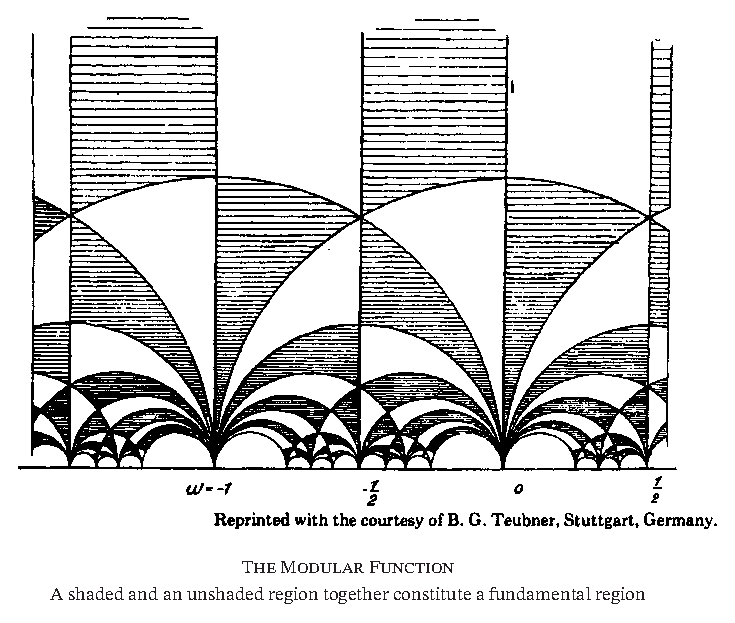
\includegraphics{chap01-vend-scan-01.eps}
\caption{Picturing paths.}\label{fig1.1.1}
\end{figure}

\noindent is a \emph{circuit}\index{circuit} (a
$k$-circuit\index{circuit!$k$-circuit} or a circuit of
length\index{circuit!of length} $k$).\footnote{Depending on
context, the notation ``$(i_{1},\ldots i_{k})$'' will denote either a
circuit or a cycle.} If $q\neq i_{1}$, then $N-\mathbf{d}\alpha=
\{q,m_{1}, m_{2},\ldots, m_{n-k-1}\}$ and
\[
\alpha=(i_{1},i_{2},\ldots,i_{k},q](m_{1}](m_{2}]\cdots(m_{n-k-1}]
\]
is a \emph{proper path}\index{proper path} $($a proper
$(k+1)$-path or a proper path of length $k+1)$.\footnote{Depending
on context, we use the notation ``$(i_{1},\ldots, i_{k},q]$'' to
denote either a proper path or the chart $(i_{1},\ldots,
i_{k},q](m_{1})\cdots(m_{n-k-1})$.}

In addition to these paths (circuits of length $\geq 1$ and proper
paths of length $\geq 2$), we define, for each $j\in N$, the
\emph{proper $1$-path}\index{proper 1-}
\[
(j]=(1](2]\cdots(n]=0\in C_{n}.
\]
We therefore have $\ell$-\emph{paths}, i.e., circuits and proper
paths\index{proper 1-} of \emph{length}\index{length paths}
$\ell\geq 1$. For example, $(1]\cdots (i-1](i)(i+1]\cdots(n]$
denotes the 1-circuit with domain $\{i\}$, while
$(12](3]\cdots(n]$ denotes the proper 2-path that maps~1 to~2.
Every path has an obvious geometrical representation
(Figure~\ref{fig1.1.1}).

\section{Building Charts from Paths}\label{sec1.2}

To build charts from paths, let $\alpha,\beta\in C_{n}$ and
suppose that $(\mathbf{d}\alpha\cup \mathbf{r}\alpha)$ and
$(\mathbf{d}\beta \cup\mathbf{r}\beta)$ are disjoint. Then
$\alpha$ and $\beta$ are \emph{disjoint} and the \emph{join}
$\gamma$ of $\alpha$ and $\beta$ (denoted
$\gamma=\alpha\beta=\beta\alpha)$ is the chart with domain
$\mathbf{d}\alpha \cup\mathbf{d}\beta$ and values determined~by
\[
x\gamma=\begin{cases}
x\alpha, & x\in \mathbf{d}\alpha\\
 x\beta, & x\in \mathbf{d}\beta.
\end{cases}
\]
So the join $\gamma=\alpha\beta$ exists if and only if $\alpha$
and $\beta$ are disjoint. For instance, the proper 2-path
$\alpha=(12](3](4]$ and the 2-circuit $\beta=(1](2](34)$ are
disjoint charts in $C_{4}$ and their join is
$\gamma=\alpha\beta=(12](34)$. Note that we did not write
$\gamma=(12](3](4](1](2](34)$, which would be confusing. It turns
out that the explicit appearance of 1-paths ``$(j]$'' is often
unnecessary. This is similar~to the case of 1-cycles in cycle
notation. To make matters worse, at times we shall also suppress
1-circuits ``$(j)$.''

Learning to multiply charts\index{circuit!in a charts} in path
notation is like learning to multiply permutations in cycle
notation, it takes a little practice. For starters, use the charts
$\alpha=(123)(45]$ and $\beta=(41)(53)(2]$ in $C_{5}$ to calculate
$\alpha \circ\beta=(1](25](34)$. Then practice taking powers of
the proper 5-path $\gamma=$ (12345] --- calculate that
$\gamma^{2}=(135](24],\gamma^{3}=(14](25](3],\gamma^{4}=(15](2](3](4]$,
and $\gamma^{5}=(1](2](3](4](5]=0$.

\section{Decomposing Charts into Paths}\label{sec1.3}

Pick any chart\index{path!in a chart} $\alpha\in C_{n}$ and
suppose that $ x\in \mathbf{d}\alpha$. We shall form some proper
paths and circuits that depend on the $\alpha$-iterates of $x$:
Let us look at the first iterate. We define
\[
\eta_{x}=(x,x\alpha]\quad \mathrm{if}\ x\alpha\neq x,\quad
\mathrm{or}\quad \gamma_{x}=(x)\quad \mathrm{if}\ x\alpha=x.
\]
Continuing with higher order iterates, for each $k\geq 2$, we
also~define
\begin{align*}
\eta_{x} &=(x, x\alpha,x\alpha^{2},\ldots, x\alpha^{k}]\quad \mathrm{when}\
\{x,x\alpha,x\alpha^{2},\ldots, x\alpha^{k}\}\ \mathrm{has\ size}\ k+1;\\
\gamma_{x} &= (x,x\alpha,x\alpha^{2},\ldots, x\alpha^{k-1})\quad \mathrm{when}\
\{x,x\alpha,x\alpha^{2},\ldots, x\alpha^{k}=x\}\ \mathrm{has\ size}\ k.
\end{align*}
Each $\eta_{x}$ is a \emph{proper path in} $\alpha$; and each
circuit $\gamma_{x}$ is a \emph{circuit in} $\alpha$. But unlike
circuits, each proper path $\eta=(i_{1}, i_{2},\ldots, i_{k}]$ has
a \emph{left-endpoint}\index{left-endpoint of proper path} $i_{1}$
and a \emph{right-endpoint}\index{right-endpoint of proper path}
$i_{k}$. Moreover, a proper path $\eta_{x}$ in $\alpha$ is
\emph{maximal} when its left endpoint $ x\in
\mathbf{d}\alpha-\mathbf{r}\alpha$ and its right endpoint $
x\alpha^{k}\in \mathbf{r}\alpha-\mathbf{d}\alpha$.

To describe how the various paths in $\alpha$ must interact, we
shall say that the path $\eta$ \emph{meets}\index{path!meets} the
path $\gamma$ whenever they are not disjoint\index{path!disjoint},
i.e.,~when
\[
(\mathbf{d}\eta\cup \mathbf{r}\eta)\cap(\mathbf{d}\gamma\cup \mathbf{r}\gamma)\neq\emptyset.
\]
To illustrate, note that the circuit (123) meets the proper 2-path
(43] at 3, while the proper paths (1234] and (5678] are disjoint.

\begin{lemma}\label{lem1.3.1}
Let $\alpha\in C_{n}$. Then the following are true:
\begin{enumerate}
 \item[(1)] For maximal paths\index{paths!maximal} $\eta$ and $\eta'$ in
$\alpha$, either $\eta=\eta'$ or $\eta$ does not meet $\eta'$.

\item[(2)] For circuits $\gamma$ and $\gamma'$ in
$\alpha$, either $\gamma=\gamma'$ or $\gamma$ does not meet
$\gamma'$.

\item[(3)] No maximal path $\eta$ in $\alpha$ meets any
circuit $\gamma$ in $\alpha$.

 \item[(4)] For each $y\in \mathbf{r}\alpha-\mathbf{d}\alpha$,
there exist $x\in\mathbf{d}\alpha-\mathbf{r}\alpha$ and $k\geq
1$ such that $x\alpha^{k}=y$, i.e., maximal $\eta_{x}=(x,
x\alpha,\ldots, x\alpha^{k}=y]$ exists whenever $y\in
\mathbf{r}\alpha-\mathbf{d}\alpha$.
\end{enumerate}
\end{lemma}

\begin{proof} Statements (1)--(3) follow since $\alpha :
\mathbf{d}\alpha\rightarrow \mathbf{r}\alpha$ is a chart. For
(4), we use induction: Since $y\in
\mathbf{r}\alpha-\mathbf{d}\alpha$, there exists $ x_{1}\in
\mathbf{d}\alpha$ such that $x_{1}\alpha=y$ and $\{x_{1},y\}$
has size two. If $x_{1}\not\in \mathbf{r}\alpha$, then,
letting $x=x_{1}$ and $k=1$, we see that $\eta_{x}=(x_{1},
y]=(x,x\alpha^{1}=y]$ is maximal. Otherwise, there exists
$x_{2}\in \mathbf{d}\alpha$ such that $x_{2}\alpha=x_{1}$ and
$\{x_{2},x_{1},y\}$ has size three. If $ x_{2}\not\in
\mathbf{r}\alpha$, then, letting $x=x_{2}$ and $k=2$, we see
that $\eta_{x}=(x_{2}, x_{1},y]=(x,x\alpha^{1},x\alpha^{2}=y]$
is maximal. But construction (by induction) of such sets
$\{x_{k},x_{k-1},\ldots, x_{1},y\}$ must terminate since $N$
is finite. It follows that the desired $x$ and $k$ exist.
\end{proof}

Next, we have the fundamental decomposition/representation
theorem.

\begin{theorem}[Unique Representation of Charts]\label{thm1.3.2}
Every chart $\alpha\in C_{n}-\{0\}$ is a (disjoint)~join
\[
\eta_{1}\cdots\eta_{u}\gamma_{1}\cdots\gamma_{v}
\]
of some (possibly none) length $\geq 2$ proper paths
$\eta_{1},\ldots, \eta_{u}$ and some (possibly none)
circuits $\gamma_{1},\ldots, \gamma_{v}$. Moreover, this
factorization is unique except for the order in which the
paths are written.
\end{theorem}

\begin{proof} If $\alpha\in C_{n}-\{0\}$, then either
$\mathbf{d}\alpha=\mathbf{r}\alpha$ or $\mathbf{d}\alpha\neq
\mathbf{r}\alpha$. In the former case, $\alpha$ is a
permutation of its domain $\mathbf{d}\alpha$, and
therefore has a disjoint ``cycle'' decomposition
\[
\alpha=\delta_{1}\circ\cdots \circ\delta_{v}\quad (\mathrm{each}\ \delta_{i}\ \mathrm{is\ a\
cycle\ on}\ \mathbf{d}\alpha).
\]
For each index $i$, let $\gamma_{i}$ be the restriction of
$\delta_{i}$ to the set of points moved by $\delta_{i}$. Then
$\alpha=\gamma_{1}\cdots\gamma_{v}$ is the desired decomposition.
In the $\mathbf{d}\alpha\neq \mathbf{r}\alpha$ case, we may
suppose that $\mathbf{d}\alpha-\mathbf{r}\alpha=\{1,2,\ldots,
u\}$. Picking $x\in \mathbf{d}\alpha-\mathbf{r}\alpha$ and
iterating, as far as possible, we obtain the~set
\[
X=\{x,x\alpha,x\alpha^{2},\ldots\}.
\]
Since $X\subset N$ is finite, there exists a minimum $k\geq 1$
such that either $x\alpha^{k}\not\in \mathbf{d}\alpha$ or
$x\alpha^{k}=x\alpha^{m}$ for minimum $m>k$. But since the case
$x\alpha^{k}=x\alpha^{m}$ is impossible because $\alpha$ is
one-one, for each $ x\in \mathbf{d}\alpha-\mathbf{r}\alpha$ there
is a $k$ such that $x\alpha^{k}\in
\mathbf{r}\alpha-\mathbf{d}\alpha$ and we can define the maximal
proper~path
\[
\eta_{x}=(x, x\alpha,\ldots, x\alpha^{k}].
\]
From (1) of~\ref{lem1.3.1}, it is clear that we can define the
join
\[
\beta=\eta_{1}\eta_{2}\cdots\eta_{u}.
\]
Thus, if $\alpha=\beta$, we are finished. Otherwise, we shall
show that a join of circuits
$\alpha'=\gamma_{1}\cdots\gamma_{v}$ exists such that
$\alpha=\beta\alpha'$: First, define
\[
\alpha'=\alpha|_{\mathbf{d}\alpha-\mathbf{d}\beta}
\]
as the restriction of $\alpha$ to
$\mathbf{d}\alpha-\mathbf{d}\beta$. To see that $\alpha'$ is a
permutation, we shall need several properties:
\begin{enumerate}
\item[(i)] $\mathbf{r}\alpha-\mathbf{d}\alpha=\mathbf{r}\beta-\mathbf{d}\beta$
(Using (4) of~\ref{lem1.3.1}, we have $ y\in
\mathbf{r}\alpha-\mathbf{d}\alpha\Leftrightarrow$ maximal
$\eta_{x}=$ ($x,\ldots, y]$ exists for some $x\in
\mathbf{d}\alpha-\mathbf{r}\alpha\Leftrightarrow y\in
\mathbf{r}\beta-\mathbf{d}\beta.$)

\item[(ii)] $\mathbf{d}\beta-\mathbf{r}\beta=\mathbf{d}\alpha-\mathbf{r}\alpha$
(Both equal $\{1,2,\ldots u\}.$)

\item[(iii)] $\mathbf{r}\alpha'\cup \mathbf{r}\beta=\mathbf{r}\alpha$.
\end{enumerate}
We can now show that $\mathbf{d}\alpha'\subset
\mathbf{r}\alpha'$, implying that $\alpha'$ is a
permutation of its domain $\mathbf{d}\alpha'$. Let $y\in
\mathbf{d}\alpha'$. Then $ y\in \mathbf{d}\alpha$ implies
$y\not\in \mathbf{r}\alpha-\mathbf{d}\alpha$. Coupling
this with $ y\not\in \mathbf{d}\beta$ and (i), we deduce
\begin{enumerate}
\item[(iv)] $y\not\in \mathbf{r}\beta$.
\end{enumerate}
Similarly, from $ y\not\in
\mathbf{d}\beta-\mathbf{r}\beta$ and $y\in
\mathbf{d}\alpha$, (ii) shows
\begin{enumerate}
\item[(v)] $ y\in \mathbf{r}\alpha$.
\end{enumerate}
Then from (iv) and (v), property (iii) yields $y\in
\mathbf{r}\alpha'$, which finishes the proof that $\alpha'$ is a
permutation.

Next, for $x\in \mathbf{d}\alpha'$, we take $\alpha$-iterates
of $x$ and get $X=\{x,x\alpha,x\alpha^{2},\ldots\}$. This
time, there exists a $k\geq 1$ such that $x=x\alpha^{k}$: For
each $x\in \mathbf{d}\alpha'$,~define
\[
\gamma_{x}=(x,x\alpha,\ldots, x\alpha^{k-1}).
\]
Then from (2) of \ref{lem1.3.1}, pairwise disjoint circuits
$\gamma_{1},\ldots, \gamma_{v}$ exist such that
$\alpha'=\gamma_{1}\cdots\gamma_{v}$. Lastly, by (3) of
\ref{lem1.3.1}, the paths in the factorization
$\alpha=\beta\alpha'=
\eta_{1}\cdots\eta_{u}\gamma_{1}\cdots\gamma_{v}$ are pairwise
disjoint.

Turning to uniqueness, we suppose that
\[
\alpha=\eta_{1}\cdots\eta_{u}\gamma_{1}\cdots\gamma_{v}
=\eta_{1}'\cdots\eta_{w}'\gamma_{1}'\cdots\gamma_{x}'
\]
has two such factorizations. If $u=0$, then
$\mathbf{d}\alpha=\mathbf{r}\alpha$, showing that $w=0$. Thus,
$\alpha=\gamma_{1}\cdots\gamma_{v}=\gamma_{1}'\cdots\gamma_{x}'$
is a join of circuits, and the uniqueness follows from an
induction argument (observe that each $\gamma_{i}$, as well as
each $\gamma_{j}'$, is a circuit in $\alpha$ and apply (2) of
\ref{lem1.3.1}). So suppose $u\geq 1$. We claim that $u=w$: First,
note that for any proper path $\eta$ of length $\geq 2$ we have
$\eta=(1,2,\ldots,
k]\Rightarrow\{1\}=\mathbf{d}\eta-\mathbf{r}\eta$. Therefore,
since the decomposition $\eta_{1}\cdots\eta_{u}$ of $\alpha$ is a
join, $\mathbf{d}\alpha-\mathbf{r}\alpha$ has $u$ elements and,
likewise, since $\eta_{1}'\cdots\eta_{w}'$ is join,
$\mathbf{d}\alpha-\mathbf{r}\alpha$ has $w$ elements, i.e., $u=w$.
So by rearrangement, if necessary, we may assume that for each
$i\,i=$ left endpoint of $\eta_{i}=$ left endpoint of $\eta_{i}'$.
But then, since each $\eta_{i}$ and each $\eta_{j}'$ are maximal,
an application of (1)~of~\ref{lem1.3.1} shows $\eta_{i}=\eta_{i}'$
for each $i$. It therefore only remains to show that we can
``cancel'' the proper paths, i.e., show~that
\[
\gamma_{1}\cdots\gamma_{v}=\gamma_{1}'\cdots\gamma_{x}',
\]
which is case $u=0$. To this end, assume that for some index
$i$, $y\in \mathbf{d}\gamma_{i}$. Then $y\not\in
\mathbf{d}(\eta_{1}\cdots\eta_{u})$ because the decomposition
is a join. This implies $y\in \mathbf{d}\gamma_{j}'$ for some
index $j$ and, consequently, $y\gamma_{i}=y\gamma_{j}'$,
showing that the function $\gamma_{1}'\cdots\gamma_{x}'$ is an
extension of $\gamma_{1}\cdots\gamma_{v}$. By a similar
argument, the latter is an extension of the former, and we
are~finished.
\end{proof}

From Theorem~\ref{thm1.3.2}, each nonzero\index{chart!zero}
$\alpha\in C_{n}$ is a disjoint join
\[
\alpha=(a_{11}\cdots a_{1k_{1}}]\cdots(a_{u1}\cdots a_{uk_{u}}]
(b_{11}\cdots b_{1m_{1}})\cdots(b_{v1}\cdots b_{vm_{v}})
\]
of proper paths of length $\geq 2$ and circuits. If
$\{j_{1},\ldots, j_{\ell}\}=N-(\mathbf{d}\alpha\,\cup\,
\mathbf{r}\alpha)$, then none of the $j_{i}$'s appear in the
representation specified in Theorem~\ref{thm1.3.2}. We may,
however, augment the Theorem~\ref{thm1.3.2} join with the proper
1-paths $(j_{i}]\,(j_{i}\not\in \mathbf{d}\alpha\,\cup\,
\mathbf{r}\alpha)$ and obtain yet another unique representation.
Indeed, augmenting the representation above, we
obtain\index{$\ell$}
\[
\alpha=(j_{1}]\cdots(j_{\ell}](a_{11}\cdots
a_{1k_{1}}]\cdots(a_{u1}\cdots a_{uk_{u}}](b_{11}\cdots
b_{1m_{1}})\cdots(b_{v1}\cdots b_{vm_{v}}),
\]
which we shall call either the \emph{path
decomposition}\index{path!decomposition $C_n$} or \emph{join
representation}\index{join representation in $C_n$} of $\alpha$.
For instance, the decomposition~of
\[
\alpha=\left(\begin{matrix}
1 & 2 & 3 & 4 & 5 & 6 & 7\\
2 & 3 & - & 5 & 4 & - & 7
\end{matrix}\right)\in C_{7}
\]
is ($123](6](45)(7)$, which may be graphically represented as in
Figure~\ref{fig1.3.3}.

\setcounter{figure}{2}
\begin{figure}[!h]
\includegraphics{chap01-vend-scan-02.eps}
\caption{The path decomposition of a chart.}\label{fig1.3.3}
\end{figure}

We also note that while the zero\index{chart!zero} chart $0$ of
$C_{n}$ is excluded from Theorem~\ref{thm1.3.2}, it does have path
decomposition $(1]\cdots (n]$. The zero $(1]\cdots (n]$ is an
example of a \emph{nilpotent}, which is a chart whose path
decomposition contains no circuits. In fact, given $\alpha\in
C_{n}$ with join representation above, its \emph{nilpotent
part}\index{nilpotent!part}~is
\[
\eta=(j_{1}]\cdots(j_{\ell}](a_{11}\cdots
a_{1k_{1}}]\cdots(a_{u1}\cdots
a_{uk_{u}}](b_{11}]\cdots(b_{1m_{1}}]\cdots(b_{v1}]\cdots(b_{vm_{v}}];
\]
and its \emph{permutation part} is
\[
\gamma=(j_{1}]\cdots(j_{\ell}](a_{11}]\cdots(a_{1k_{1}}]\cdots(a_{uk_{u}}](b_{11}\cdots
b_{1m_{1}})\cdots(b_{v1}\cdots b_{vm_{v}}).
\]
In other words, each chart $\alpha=\eta\gamma$ is the join of its
nilpotent and permutation parts\index{permutation(s)~part}. In
particular, the chart $\alpha=(123](6](45)(7)$ pictured in
Figure~\ref{fig1.3.3} has nilpotent part
$\eta=(123](6]=(123](6](4](5](7]$ and permutation part
$\gamma=(45)(7)=(45)(7)(1](2](3](6]$.

\section{Comments}\label{sec1.4}

As one might suspect, the literature on semigroups is rather
diverse with certain of its areas extensively developed.
Hille's\index{Hille, E.} book concerns the \emph{analytic
theory}\index{semigroups!analytic} of semigroups and its
\emph{applications to analysis}, while Birkhoff's\index{Birkhoff}
text gives an account of
\emph{lattice-ordered}\index{lattice-ordered} semigroups. On the
other hand, the books by Suschkewitsch,\index{Suschkewitsch, A.K.}
Ljapin,\index{Ljapin, E.S.} and Clifford\index{Clifford, A.H.} and
Preston concern \emph{algebraic semigroups}\index{algebraic
theory} --- those semigroups not endowed with any further
structure.

Historically, it is claimed that the term ``semigroup'' first
appeared in the mathematical literature in 1904 (page 8 of J.-A.
de S\'{e}guier's\index{S\'{e}guier, J.-A. de} book
[\ref{bib70}]), that the first published paper
on semigroups appeared in 1905 (L. E. Dickson\index{Dickson L. E.}
[\ref{bib12}]), and that the first book on
semigroups appeared in 1937 (A. K.
Suschkewitsch\index{Suschkewitsch,
A.K.}~[\ref{bib73a}]). (Clifford and
Preston\index{Preston, G.B.}~[\ref{bib8}] and
also Schein\index{Schein, B.M.}~[\ref{bib69}].)

From 1940 to 1961, according to Clifford and Preston, ``$\ldots$
the number of papers [on semigroups] appearing each year has grown
fairly steadily to a little more than 30 on average.'' Their
estimate roughly equates to the 494 bibliographical entries in the
1958 (first) edition of Ljapin's\index{Ljapin, E.S.}
book~[\ref{bib46}].

In 1952, Wagner introduced inverse semigroups as \emph{generalized
groups}, and two years later, in 1954, Preston independently
discovered these semigroups, calling them\index{inverse}
\emph{inverse semi-groups}\index{inverse semi-groups}.
Subsequently, research activity in inverse semigroups was
substantial: In 1984, M. Petrich published his 674-page text,
\emph{Inverse Semigroups}\index{inverse semigroups}. It contains
546 bibliographical entries, 505 of which are dated after 1958,
the year that Ljapin listed~494.

At the very beginnings of inverse semigroup theory,
Wagner\index{Wagner, V.V.} [\ref{bib78}] in
1952, Preston\index{Preston, G.B.}
[\ref{bib63a}] in 1954, and
Preston\index{Preston, G.B.} [\ref{bib63b}] in
1957, proved the Wagner-Preston Theorem --- each inverse semigroup
is isomorphic to a subsemigroup of a symmetric\index{symmetric}
inverse semigroup
--- the analogue of Cayley's Theorem\index{Cayley's Theorem}.

Also in 1957, as part of his study of characters of symmetric
inverse semigroups, W. D. Munn\index{Munn, W.D.}
[\ref{bib54}] was the first to discover a
notational representation of charts that is essentially equivalent
to path decomposition.

Munn's decomposition used ``links'' and ``cycles,'' instead of
proper paths and circuits. For example, given the chart $(18](29](345)(6)(7) \in C_{9}$,
he would write [18][29](345)(6)(7), the
links being [18] and [29]. Links were defined as sequences. Thus,
for example, [18] would be a map having domain of size~2. In the
context of path notation, however, (18] is a proper 2-path, having
domain of size 1. Similarly, the 3-circuit ``(345)''  has domain
of size 3, while in the context of Munn's notation, ``(345)'' is a
cycle with domain of size 9. In spite of these differences, Munn's
approach and the one used here yield essentially the same
notational~form.

By the mid-1980s, the idea of a proper path was evidently an idea
waiting to happen: In 1986, the author
[\ref{bib37}] independently invented path
notation (as presented here) and proved Theorem~\ref{thm1.3.2}.
(The approach grew out of a study of hypomorphic mapping sets in
the famous Graph Reconstruction Conjecture
(Chapter~\ref{chap13}).$)$ In the next year (1987), G. M. S.
Gomes\index{Gomes, G. M. S.} and J. H. Howie\index{Howie, J. M.}
[\ref{bib22a}] independently introduced the
notion of a \emph{primitive nilpotent}, which they denoted
``$||12\cdots k||$.'' (Unlike ``links,'' primitive nilpotents are
precisely proper paths.) In their Theorem~2.8, they show that a
non-zero nilpotent in $C_{n}$ is a disjoint union of primitive
nilpotents, which is part of our Theorem~\ref{thm1.3.2}. And also
in 1987, R. P. Sullivan\index{Sullivan, R.P.}
[\ref{bib72}] independently defined
$k$-\emph{chains} ``$[1,\ldots, k+1]$'' and $k$-\emph{cycles}
``($1,\ldots,k$)'', which are, respectively, proper $(k+1)$ paths
and $k$-circuits.

This mid-1980s idea of decomposing charts into paths merits
comparison with the 1815 idea of decomposing permutations into
cycles. In the permutation case, cycle decomposition appeared in
1815 along with the beginnings of finite group theory. In
particular, in 1815 Cauchy [\ref{bib7}]
introduced cycle notation ``$(i,j)$'' for transpositions, factored
a three cycle $(i,j,k)=(j,k)\circ (i,j)$, and then (Cauchy
[\ref{bib7a}]) decomposed permutations into
disjoint cycles. Cycle notation proved useful in the early (up to
1911) development of finite group theory: Burnside\index{Burnside
W.} [\ref{bib6}] opens his 1911 text
\emph{Theory of Groups of Finite Order} with the following comment
on cycle notation,
\begin{quote}
``AMONG the various notations used in the following pages, there
is one of such frequent recurrence that a certain readiness in its
use is very desirable in dealing with the subject of this
treatise. We therefore propose to devote a preliminary chapter to
explaining it in some detail.''
\end{quote}

Since 1911, however, the approach to group theory has become more
and more abstract, requiring less and less cycle notation.
Nevertheless, cycle notation remains useful, if not fundamental,
to the $S_{n}$~theory.

In contrast, conceived in the 1950s, inverse semigroup theory was
axiomatic from its inception. It has the $C_{n}$ theory as one of
its branches and path notation did not appear until the mid-1980s.
As to the state of the $C_{n}$ theory in 1985, consider the
following statement of Gomes\index{Gomes, G. M. S.} and
Howie\index{Howie, J. M.} [\ref{bib22}]:
\begin{quote}
``Since the theory of inverse semigroups is now extensive enough
to have been the subject of a substantial book by Petrich
[\ref{bib60}], it is perhaps rather surprising
that very little has been written on the symmetric inverse
semigroup.''
\end{quote}

\chapter{Basic Observations}\label{chap2}

For the $S_{n}$ theory, Cauchy's convenient and flexible cycle
notation is a seminal, even fundamental, way of thinking. In a
similar vein, for the $C_{n}$ theory, path notation also provides
a fundamental way of thinking.\footnote{In the chapter \emph{Path
Notation for Partial Transformations}, we shall see how path
notation extends from the symmetric inverse semigroups $C_{n}$ to
the more general partial transformation semigroups $PT_{n}$.}

In this chapter, we present the path notation view of idempotent,
nilpotent, and inverse charts. Conjugacy and path structure are
introduced and connected, extending their group counterparts (from
$S_{n}$ to $C_{n}$). This connection is used to compute the
conjugacy classes of $C_{4}$ (Table~\ref{tab2.7.1}). Path notation
is also applied to finite cyclic semigroups, thereby generalizing
Ruffini's classical result [\ref{bib66}] that
the order of a permutation is the least common multiple of the
order of its cycles. For completeness of the cyclic semigroup
theory, we sharpen Frobenius' result\index{Frobenius
result} [\ref{bib17}].

\setcounter{section}{4}
\section{Idempotents, Nilpotents, Inverses, Conjugacy}\label{sec2.5}

First, recall that an element $e$ in a semigroup $S$ is an
\emph{idempotent}\index{idempotent} if $e^{2}=e$. For example,
each $S_{n}$, indeed any group, contains exactly one idempotent
while each $C_{n}$ contains several idempotents. For $C_{3}$ in
particular, if $i,j,k$ denote distinct members of $\{1, 2, 3\}$,
then for idempotents we have one of rank 3, three of rank 2, three
of rank 1, and one of rank~$0$:
\[
\begin{matrix}
\mathrm{rank}\ 3 &\mathrm{rank}\ 2 &\mathrm{rank}\ 1 &\mathrm{rank}\ 0 \\
(1)(2)(3) &(i)(j)(k] &(i)(j](k] &(1](2](3]
\end{matrix}
\]
That each of these idempotents is a join of 1-paths is no
accident.

Second, recall that an element $a$ in a semigroup $S$ with zero
``$0$'' is a \emph{nilpotent}\index{nilpotent(s)} if one of its
positive powers $a^{k}$ is zero, i.e., $a^{k}=0$ for some positive
integer $k$. For example, each $S_{n} (n\geq 2)$ contains no
nilpotents (since nontrivial groups contain no zero) while each
$C_{n}$ is rich in nilpotents. For $C_{3}$ in particular, we find
nilpotents at several ranks, namely, six of rank 2, six of rank 1,
and one of rank~$0$:
\[
\begin{matrix}
\mathrm{rank}\ 3 &\mathrm{rank}\ 2 &\mathrm{rank}\ 1 &\mathrm{rank}\ 0 \\
\mathrm{none} &(ijk] &(ij](k] &(1](2](3]
\end{matrix}
\]
That these nilpotents are joins of proper paths is no accident.

Third, recall that a chart $\beta$ is the \emph{inverse} of a
chart $\alpha$ if $\beta : \mathbf{r}\alpha\rightarrow
\mathbf{d}\alpha$ is the inverse (function) of $\alpha$. In such a
case, we write $\beta=\alpha^{-1}$. As we shall see, ``reversing
paths'' switches between a chart and its inverse, just as
``reversing cycles'' switches between a permutation and
its~inverse.

Finally, to extend (from $S_{n}$ to $C_{n}$\index{idempotent(s)!in
$C_{n}$}) the equivalence \emph{Two permutations are conjugate if
and only if they have the same cycle structure}, we need the
following: For $\alpha,\beta\in C_{n}$, we say $\alpha$ is
\emph{conjugate} to $\beta$ whenever there exists a permutation
$\gamma\in S_{n}$ such that $\gamma^{-1}\alpha\gamma=\beta$.
Moreover, if $\alpha=\alpha_{1}\cdots\alpha_{k}$ and
$\beta=\beta_{1}\cdots\beta_{m}$ are join representations, then
$\alpha$ and $\beta$ have the \emph{same path structure} whenever
$k=m$ and there exists a permutation $\phi$ of $K= \{1,2,\ldots,
k\}$ satisfying, for each $i\in K$,
\begin{enumerate}
\item[(i)] length of $\alpha_{i}= \mathrm{length}$ of $\beta_{i\phi}$, and

\item[(ii)] $\alpha_{i}$ is a proper path if and only if $\beta_{i\phi}$
is a proper~path.
\end{enumerate}
So
$\alpha=(123](45](678)(9)=\alpha_{1}\alpha_{2}\alpha_{3}\alpha_{4}\in
C_{9}$ and $\beta=(67](489](1)(235)=
\beta_{1}\beta_{2}\beta_{3}\beta_{4}\in C_{9}$ have the same path
structure because (the matching of paths) $\phi =(12)(34)$
satisfies ($i$) and (\emph{ii}). Furthermore, we may use this
$\phi$ to show that $\alpha$ is conjugate to $\beta$: First, as
indicated below, place each $\alpha_{i}$ over $\beta_{i\phi}$ ---
\begin{align*}
\alpha_{1}\alpha_{2}\alpha_{3}\alpha_{4}&=(123](45](678)(9) \\
\beta_{2}\beta_{1}\beta_{4}\beta_{3}&=(489](67](235)(1).
\end{align*}
Second, define $\gamma\in S_{9}$ via ``first-to-second line
vertical inspection,'' i.e, $\gamma$ is given by $1\mapsto
4,2\mapsto 8,\ldots.$ From the definition of $\gamma$, we have
\[
\gamma^{-1}\alpha\gamma=\beta.
\]
In other words, $\alpha$ moves $i$ to $j$ if and only if $\beta$
moves $i\gamma$ to $j\gamma$. That $\alpha$ and $\beta$ are
conjugate whenever they have the same path structure is no
accident.

\begin{theorem}\label{thm2.5.1}
Let $\alpha,\beta,\eta\in C_{n}$ and let $\alpha$ have path
decomposition $\eta_{1}\cdots\eta_{u}\gamma_{1}\cdots\gamma_{v}$
where each $\eta_{i}$ is a proper path and each $\gamma_{i}$ is a
circuit. Then the following statements are true.
\begin{enumerate}
\item[(1)] Chart $\alpha$ is an idempotent if and only if
each path in the join representation of $\alpha$ has length
one.

\item[(2)] Chart $\alpha$ is nilpotent if and only if each
path in the join representation of $\alpha$ is a proper path.

\item[(3)] The decomposition of $\alpha^{-1}$ is
$\eta_{1}^{-1}\cdots\eta_{u}^{-1}\gamma_{1}^{-1}\cdots\gamma_{v}^{-1}$
where for proper paths,
($i_{1},\ldots,i_{k}]^{-1}=(i_{k},\ldots, i_{2},i_{1}]$, and
for circuits, $(j_{1},\ldots,
j_{k})^{-1}=(j_{k},\ldots,j_{2},j_{1})$.

\item[(4)] Chart $\alpha$ is conjugate to chart $\beta$
if and only if $\alpha$ and $\beta$ have the same path
structure.

\item[(5)] For a proper path $\eta=(i_{1}, i_{2},\ldots, i_{k}]$
of length $k\geq 2$, we have $\eta^{k}=0$ but, for each
positive integer $m<k,\eta^{m}\neq 0$.

\item[(6)] For any nonzero integer $k$, we may calculate the
$kth$ power of $\alpha$ using
$\alpha^{k}=\eta_{1}^{k}\cdots\eta_{u}^{k}\gamma_{1}^{k}\cdots\gamma_{v}^{k}$.
\end{enumerate}
\end{theorem}

\begin{proof} To prove (1), use $i\alpha\neq i$, for $i\in
\mathbf{d}\alpha$, implies $ i\alpha^{2}\neq i\alpha$. To prove
(2), observe that $\alpha=\eta\gamma$ has a permutation part
$\gamma$ if and only if $\alpha^{n}\neq 0$ for every $n\geq 1$. To
prove (3), use $i\alpha=j$ if and only if $j\alpha^{-1}=i$, and
then recall that the path decomposition of $\alpha^{-1}$ is
unique. For (4), first show that conjugates $\alpha$ and $\beta$
necessarily have the same path structure by observing that any
conjugate of an $\ell$-circuit is an $\ell$-circuit, and any
conjugate of a proper $\ell$-path is a proper $\ell$-path. Second,
show that charts\index{charts} $\alpha$ and $\beta$ having the
same path structure are conjugate by formalizing the argument
given in the paragraph preceding this theorem. To prove (5),
observe that $1\leq m<k$ implies $i_{1}\eta^{m}=i_{m+1}$, and,
since $\eta^{k}=\eta^{k-1}\eta$, that the domain
$\mathbf{d}(\eta^{k})$ of $\eta^{k}$ is empty. To prove (6),
recall that the paths appearing in the decomposition of $\alpha$
are pairwise disjoint.
\end{proof}

In light of Theorem~\ref{thm2.5.1}, it is instructive to verify
that $C_{n}$ is an inverse (and hence regular) semigroup. Recall
that a semigroup $S$ is an \emph{inverse semigroup}\index{inverse
semigroup} if every element has a unique inverse, i.e., for each
$a\in S$, there exists a unique solution $x\in S$ of the system
$axa=a,\ xax=x$. An equivalent definition is that $S$ is a regular
semigroup whose idempotents commute. (A semigroup $S$ is
\emph{regular}\index{regular} if each of its elements is regular,
i.e., for each $a\in S$, there exists $x\in S$ such that $axa=a.$)

\section{Index and Period of a Chart}\label{sec2.6}

If $a$ is any element in any semigroup $S$, then the \emph{cyclic
subsemigroup} $\langle a\rangle$ of $S$ \emph{generated by} a
consists of all positive integral powers of $a$. The \emph{order}
of $a$ is the order of $\langle a\rangle$. Since we shall only
consider finite cyclic semigroups $\langle a\rangle$, there exist
positive integers $r$ and $s$ with $r<s$ such that $a^{r}=a^{s}$.
Moreover, if $s$ is the smallest such positive integer, then
$a,a^{2},\ldots,a^{s-1}$ are distinct and $r$ is the only integer
less than $s$ with $a^{r}=a^{s}$. The integer $r$ is called the
\emph{index}\index{chart!index} and $m=s-r$ the
\emph{period}\index{chart!period} of $a$ (of $\langle a\rangle)$. We
always have $\emph{index} +\emph{period}
=\emph{order}+1$,\index{chart!order} and the subsemigroup
$K_{a}=\{a^{r},a^{r+1},\ldots, a^{r+m-1}\}$ of $S$ is a cyclic
group of order $m$. Each finite $\langle a\rangle$ contains
exactly one idempotent, namely, the identity element of~$K_{a}$.

The key relation between $\langle a\rangle$ and $C_{n}$ is
illustrated in Figure~\ref{fig2.6.1}, which pictures an
isomorphism between an abstract cyclic semigroup $\langle
a\rangle$, of index 3 and period 4, and
$\langle(123](4567)\rangle\in C_{7}$.

\begin{figure}[!h]
\includegraphics{chap02-vend-scan-01.eps}
\caption{A cyclic semigroup isomorphism.}\label{fig2.6.1}
\end{figure}

In addition to such isomorphisms, the ideas developed below are
best motivated by simple examples: Calculate the period of
$\alpha=(12)(345)(6789]\in C_{9}$ and the index of
$\eta=(12](345](6789]$, the former being the least common multiple
of 2 and 3, while the latter is the maximum of 2, 3, and 4. Then
calculate the idempotents $\alpha^{6}=(1)(2)(3)(4)(5)(6](7](8](9]$
and $\eta^{4}=0\in C_{9}$.

\setcounter{equation}{1}
\begin{proposition}\label{prop2.6.2}
Let $\langle a \rangle$ be any finite cyclic semigroup with index
$r$ and period\index{chart!index, period, order} $m$. Then
\begin{enumerate}
 \item[(1)] the cyclic semigroup $\langle a\rangle$ is
isomorphic to the cyclic subsemigroup $\langle
(1,2,\ldots,r](r+1,r+2,\ldots, r+m)\rangle\subset C_{r+m}$
generated by $\alpha= (1,2,\ldots, r](r+1,\ldots, r+m)$; and

 \item[(2)] the smallest exponent $k$ such that $a^{k}$
is the identity of $K_{a}$ is the smallest $k\geq r$ that is
also a multiple of~$m$.
\end{enumerate}
\end{proposition}

\begin{proof} Suppose $\langle a\rangle$ has index $r$ and period $m$. To see
(1), first calculate that $\langle(1,2,\ldots,  r](r+1,\ldots,
r+m)\rangle$ has index $r$ and period $m$. Then observe that
$a\mapsto(1,2,\ldots, r](r+1,\ldots, r+m)$ induces the desired
isomorphism. To see (2), apply the isomorphism: For each
$k=1,2,\ldots$, we see that $a^{k}$ corresponds to
$\alpha^{k}=(1,2,\ldots, r]^{k}(r+1,\ldots,r+m)^{k}$. By (1) of
Theorem~\ref{thm2.5.1}, $\alpha^{k}$ is an idempotent if and only
if $\alpha^{k}$ is a join of 1-paths. So $k$ is an exponent such
that $a^{k}$ is the identity of $K_{a}$ if and only~if
\begin{align*}
(1, 2,\ldots,r]^{k}&=0=(1](2]\cdots(r]\ \mathrm{and}\\
(r+1,r+2,\ldots, r+m)^{k}&=(r+1)(r+2)\cdots(r+m).
\end{align*}
But the first equation is equivalent to $k\geq r$, while the
second is equivalent to $k$ being a multiple of $m$. Thus, the
smallest exponent $k$ such that $a^{k}$ is the identity of $K_{a}$
is also the smallest $k\geq r$ that is also a multiple of $m$.
\end{proof}

\begin{theorem}\label{thm2.6.3}
Let $\alpha\in C_{n}$. Then the following statements are true.
\begin{enumerate}
\item[(1)] The index\index{chart!index, period, order} of $\alpha$ is the maximum of the
lengths of the proper paths appearing in its join
representation. If no proper paths appear, then its index is one.

\item[(2)] The period of $\alpha$ is the least common
multiple of the lengths of the circuits appearing in its join
representation. If no circuits appear, then its period is one.
\end{enumerate}
\end{theorem}

\begin{proof} For (1), if no proper paths appear in the join
representation of $\alpha\in C_{n}$, then $\alpha\in S_{n}$ is a
permutation and the index of $\alpha$ is obviously one while the
order of $\alpha$ is just the period of $\alpha$. That the index
of an $\alpha\in C_{n}-S_{n}$ can be calculated as claimed, we
merely apply (5) and (6) of Theorem~\ref{thm2.5.1}. For the proof
of (2), suppose $\alpha$ has an $\ell$-circuit $\gamma$ in its
decomposition. Then, since $\gamma^{k}$ can be an idempotent only
when $k$ is a multiple of $\ell$, it follows from (6) of
\ref{thm2.5.1} that the period of $\alpha$ is the least common
multiple of the lengths of the circuits appearing in the
decomposition of $\alpha$. On the other hand, if no circuits
appear, then $\alpha^{k}$ is $0$ for some $k$ and the period is one.
\end{proof}

If $\alpha\in S_{n}$, then (2) of \ref{thm2.6.3} specializes to
Ruffini's result:\index{Ruffini's result} \emph{The order of} a
\emph{permutation is the least common multiple of the lengths of
its cycles}.

\begin{corollary}\label{cor2.6.4}
Let $\langle a\rangle$ be a cyclic semigroup with index $r$ and
period $m$. If $q=\lfloor(r-1)/m\rfloor$ is the integer part of
$(r-1)/m$, then $k= (q+1)m$ is the smallest integer such that
$a^{k}$ is the identity in $K_{a}$.
\end{corollary}

\begin{proof}
From \ref{prop2.6.2}, it suffices to show that $k$ is the smallest
multiple of $m$ such that $k\geq r$. First, $k-m =qm<r$: This
follows~from
\[
qm=\left\lfloor\frac{r-1}{m}\right\rfloor m\leq\frac{r-1}{m}m=r-1<r.
\]
Second, $k=qm+m\geq r$: Now $r-1 =\ell m+t$ for some $t,0\leq
t<m$. Then,
\begin{gather*}
\textstyle\left\lfloor\frac{r-1}{m}\right\rfloor=\left\lfloor\frac{\ell
m+t}{m}\right\rfloor=\left\lfloor
\ell+\frac{t}{m}\right\rfloor=\ell=\frac{r-1-t}{m},\quad
\mathrm{showing\ that}\\
\textstyle k=qm+m=\left\lfloor\frac{r-1}{m}\right\rfloor
m+m=\frac{r-1-t}{m}m+m=r-1-t+m\geq r,
\end{gather*}
which finishes the proof.
\end{proof}

In the next section, we consider the cyclic subsemigroups
of~$C_{4}$.

\section{Cyclic Subsemigroups of $C_{n}$}\label{sec2.7}

Expressing $\alpha\in C_{n}$ in its join representation, we
``know'' (via Theorem~\ref{thm2.6.3}) the index and period of
$\alpha$, i.e., we know $\langle\alpha\rangle$ up to isomorphism.
As a consequence, the isomorphism classes of cyclic subsemigroups
of $C_{n}$ can be determined by listing all possible forms of join
representations.

In addition, a conjugacy class of $C_{4}$ is just the set of all
charts in $C_{4}$ having a given path structure. It follows that
each ``path structure form''
\[
(\cdots]\cdots(\cdots](\cdots)\cdots(\cdots)
\]
determines, and is determined by, a conjugacy class.

\begin{table}[!h]
\caption{Path structure of charts in $C_{4}$.}\label{tab2.7.1}
{\begin{tabular}{@{}|l|c|c|c|c|@{}} \hline
\multicolumn{1}{|l|}{\textbf{number of} $m\rightarrow m$ \textbf{maps}}&  \multicolumn{1}{|l|}{\textbf{path structure}}&   \multicolumn{1}{|l|}{\textbf{number}}& \multicolumn{1}{|l|}{\textbf{index}}& \multicolumn{1}{|l|}{\textbf{period}} \\
\hline
\multicolumn{1}{|l|}{$\big(\!\begin{smallmatrix}4 \\ 0\end{smallmatrix}\!\big)^{2}\,0!=1$} &(1](2](3](4] &1 &1 &1 \\
\hline
\multicolumn{1}{|l|}{$\big(\!\begin{smallmatrix} 4\\ 1\end{smallmatrix}\!\big)^{2}\,1!=16$} &(1)(2](3](4] &4 &1 &1 \\
&(12](3](4] &12 &2 &1 \\
\hline
\multicolumn{1}{|l|}{$\big(\!\begin{smallmatrix}4\\ 2\end{smallmatrix}\!\big)^{2}\,2!=72$}&(1)(2)(3](4]& 6&1&1 \\
&(12)(3](4]&6&1&2 \\
&(12](3)(4]& 24&2&1 \\
& (123](4] &24&3&1 \\
& (13](24]&12&2&1 \\
\hline
\multicolumn{1}{|l|}{$\big(\!\begin{smallmatrix}4\\ 3\end{smallmatrix}\!\big)^{2}\,3!=96$}& (1)(2)(3)(4]&4&1&1 \\
&(12)(3)(4]&12&1&2 \\
& (123)(4] &8&1&3 \\
&(12](3)(4)&12 &2&1 \\
& (12](34)&12 &2&2 \\
& (123](4) &24 &3&1 \\
&(1234]&24&4&1  \\
\hline
\multicolumn{1}{|l|}{$\big(\!\begin{smallmatrix}4\\ 4\end{smallmatrix}\!\big)^{2}\,4!=24$}&(1)(2)(3)(4)&1&1&1 \\
&(12)(3)(4)&6&1&2 \\
&(123)(4)&8&1&3 \\
&(1234)&6&1&4 \\
& (12)(34)&3&1&2 \\
\hline
&\multicolumn{2}{|c|}{$\mathbf{Total} = \qquad\quad \mathbf{209}$} & & \\
 \hline
\end{tabular}}{}
\end{table}

Thus, since Table~\ref{tab2.7.1} contains all possible path
structure forms for charts in $C_{4}$, we conclude that $C_{4}$
has 20 conjugacy classes. As to the size of each of these
conjugacy classes\index{chart!conjugacy classes of}, we need only
look under the column headed ``number.'' And using the columns
headed ``index'' and ``period,'' we see that these conjugacy
classes combine to form eight isomorphism classes. Recall that the
number of charts in $C_{4}$~is
\[
\sum\nolimits_{m=0}^{4}\ \big(\!\begin{smallmatrix}
4\\
m
\end{smallmatrix}\!\big)^2 m!=209.
\]

\section{Comments}\label{sec2.8}

Both finite group theory and cycle notation date from the time of
Cauchy\index{Cauchy, A.L.}. For the development of finite group
theory prior to 1911, see W. Burnside's\index{Burnside W.} text
[\ref{bib6}], and for many of the developments
after 1911, see any standard reference, e.g., Suzuki\index{Suzuki,
M.} [\ref{bib74}] and
[\ref{bib74a}]. As for cycle notation, inspired
by Gauss'\index{Gauss, C. F.} use of ``the theory of forms,''
Cauchy introduced the notation in his 1815 memoir (Cauchy
[\ref{bib7}]
and~[\ref{bib7a}]).

One benefit of cycle notation is that in $S_{n}$, cycle structure
determines conjugacy. This result is rather old, appearing as a
''first principle'' in \S\ref{sec7.32} of C.
Jordan's\index{Jordan, C.} 1870 text
[\ref{bib34}], while its (obvious) extension to
$C_{n}$\index{cyclic!in $C_{n}$}, that path structure determines
conjugacy, is rather new, introduced in 1992 by the author
[\ref{bib43d}]. By 1995, the more general view
of conjugacy was fundamental to classifying the $S_{n}$-normal
semigroups (Chapter~\ref{chap7}).

As for conjugacy in arbitrary semigroups, there seems to be no
standard. One definition is given in Dauns
[\ref{bib10}], where semigroups with a zero have
every pair of elements conjugate, two equivalent definitions
appear in Lallement\index{Lallement, G.}\index{Lallement's
Question} [\ref{bib38}], which concern words in
a free semigroup, and yet another in Goldstein\index{Goldstein,
R.} and Teymouri\index{Teymouri, J.}
[\ref{bib21}], which is a modification of the
one used by Lallement. Moreover, when the two equivalent
definitions of conjugacy used by Lallement are extended to
arbitrary monoids, they become different concepts
(Zhang\index{Zhang, L.} [\ref{bib80}]
and~[\ref{bib80a}]).

While~\ref{lem1.3.1} extends to $C_{n}$ the unique representations
enjoyed in $S_{n}$, Theorem~\ref{thm2.5.1} extends to $C_{n}$ the
well known ``algebra of cycle notation''\index{algebra of cycle
notation} that allows one to ``see (or anticipate) the basics.''
For example, consider the following:
\begin{enumerate}
\item[(i)] With (1) of \ref{thm2.5.1}, which says that idempotents are joins of
1-paths, we shall ``see'' in \S\ref{sec3.10} that idempotents
in any finite inverse semigroup~commute.

\item[(ii)] With (2) of \ref{thm2.5.1}, which says that nilpotents are joins of
proper paths, we ``see'' the following proposition because we
``essentially see'' the proper paths ``moving $A$ to the
right,'' and not ``fixing $A$,'' which would require circuits
in the representation of~$\alpha$.

\item[]A chart $\alpha\in C_{n}$ of rank $k<n$ is nilpotent if and
only if there exists no nonempty subset $A$ of
$\mathbf{d}\alpha$ such that $A\alpha= A$.


\item[(iii)] With (3) and (4) of \ref{thm2.5.1}, we ``see'' that $\alpha^{-1}$ and
$\alpha$ are conjugate charts. Moreover, we may easily find
$\beta\in S_{n}$ such that
$\beta^{-1}\alpha\beta=\alpha^{-1}$, which would be rather
tedious without the notation.

\item[(iv)] With (5) and (6) of \ref{thm2.5.1}, we have pictures such as Figure~\ref{fig2.6.1},
where we ``see,'' or may easily predict, the behavior of
powers of charts without performing any multiplications.
\end{enumerate}

For idempotents in other semigroups, in 1966 Howie
[\ref{bib22a}] published a seminal paper where
he characterized the elements of $T_{X}$, the semigroup (under
composition) of all total transformations $X\rightarrow X$, that
may be written as a product of idempotents in $T_{X}$. His work
was extended to $PT_{X}$, the semigroup (under composition) of all
partial (not necessarily one-one) transformations $X\rightarrow
X$, for finite $X$ in 1969 by Sullivan\index{Sullivan, R.P.}
[\ref{bib72a}], and, independently, in 1970 and
1972 for arbitrary $X$ by Evseev\index{Evseev, J. A.} and
Podran\index{Podran N.E.} [\ref{bib15}] and
[\ref{bib15a}]. For other examples and
information on research in this area, see Howie's 1980 and 1984
papers [\ref{bib31b}] and [\ref{bib31c}], see the introduction of
Sullivan's\index{Sullivan, R.P.} 1987 paper
[\ref{bib72}], and Saito's\index{Saito, T.} 1989
papers [\ref{bib67}]
and~[\ref{bib67a}].

Nilpotents do not appear as elements of groups because nontrivial
groups have no zero. If a finite transformation semigroup $S$
contains a zero, then it contains nilpotents, and it is natural to
ask about the subsemigroup of $S$ generated by all the nilpotents
in $S$. In 1987, Gomes\index{Gomes, G. M. S.} and Howie\index{Howie,
J. M.} [\ref{bib22a}] and
Sullivan\index{Sullivan, R.P.} [\ref{bib72}]
independently initiated this study for $C_{n}$ and $PT_{n}$,
respectively. (Recall that $PT_{n}$ denotes the semigroup of all
partial (not necessarily one-one) transformations $N\rightarrow
N$.) Nilpotents have also been studied in other special cases,
e.g., for a recent (1994) reference see Garba\index{Garba, G.
U.}~[\ref{bib18}].

The notion of regularity was introduced into ring theory in 1936
by J. von Neumann\index{von Neumann, J.}. In the general theory of
semigroups, regular semigroups were first studied by
Thierrin\index{Thierrin, G.} [\ref{bib76}] in
1951 under the name of \emph{demi-groupes inversifs}.

Regular semigroups with commuting idempotents became important in
1952 when Wagner [\ref{bib78}] introduced
inverse semigroups. In 1952 and 1954, respectively, Wagner
[\ref{bib78}] and Preston\index{Preston, G.B.}
[\ref{bib63}] independently showed that a
regular semigroup with commuting idempotents is an inverse
semigroup. In 1953, Liber\index{Liber, A.E.}
[\ref{bib42}] proved the converse
--- any inverse semigroup is necessarily regular with commuting
idempotents. Equivalent results were obtained in 1955 by Munn and
Penrose\index{Penrose R.}~[\ref{bib55}].

It was G. Frobenius\index{Frobenius, G.}
[\ref{bib17}] in 1895 who first characterized
the smallest exponent $k$ such that $a^{k}$ is the identity of
$K_{a}$ as the positive integer $k$ satisfying $m|k$ and $r\leq
k<r+m$. That every element $a$ in every finite semigroup determines
a $k$ such that $a^{k}$ is idempotent was also proved in 1902 by
E. H. Moore\index{Moore, E.H.}~[\ref{bib53a}].
Corollary~\ref{cor2.6.4}, which provides a formula $k=k(r,m)$ for
calculating $k$, was discovered by the author
[\ref{bib43}]. The results of Frobenius were
also found by Morgan Ward in 1933 (unpublished);
Suschkewitsch\index{Suschkewitsch,
A.K.}~[\ref{bib73a}, \S\ref{sec5.19} of
Chapter~\ref{chap2}] (1937); Poole\index{Poole, A.R.}
[\ref{bib61}] (1937); Rees\index{Rees, D.}
[\ref{bib23}] (1940); and
Climescu\index{Climescu, A.C.} [\ref{bib9}]
(1946).

In the $S_{n}$ theory, it is standard practice
(Rotman\index{Rotman, J.J.} [\ref{bib65}, pages
41--44]) to use cycle notation to catalog conjugacy classes
and/or count cyclic subgroups. The extension of such catalogs to
include $C_{n}$ (Table~\ref{tab2.7.1}) was natural---path
structure determines both the conjugacy classes in $C_{n}$ and the
isomorphism classes of cyclic subsemigroups of $C_{n}$
(Theorem~\ref{thm2.6.3}).

\chapter{Commuting Charts}\label{chap3}

We generalize the classical (circa 1870) characterization of
commuting permutations --- if $\alpha,\beta\in S_{n}$ and $\alpha$
has disjoint cycle decomposition $\gamma_{1}\cdots\gamma_{v}$,
then $\alpha\circ\beta=\beta \circ\alpha$ if and only if $\beta$
maps each $\gamma_{i}$ onto a $\gamma_{j}$ of the same length,
preserving the $\alpha$-induced cyclic ordering. The
generalization necessarily concerns both the nilpotent and
permutation parts of a chart --- if $\alpha,\beta\in C_{n}$ and
$\alpha$ has path decomposition
$\eta_{1}\cdots\eta_{u}\gamma_{1}\cdots\gamma_{v}$, then $\alpha
\circ\beta=\beta \circ\alpha$ if and only if $\beta$ maps some
(possibly none) of the circuits $\gamma_{i}$ onto some of the
$\gamma_{i}$, preserving both length and $\alpha$-induced cyclic
ordering, and, in addition, $\beta$ also maps some (possibly none)
\emph{initial segments}\index{initial segments of} of the
$\eta_{j}$ onto some \emph{terminal segments}\index{terminal
segments} of the $\eta_{j}$, preserving the $\alpha$-induced
linear ordering.

We begin with examples of mappings of circuits and segments
(\S\ref{sec3.9}). Following the examples, we formalize the idea of
initial and terminal segments of a proper path, and then make
precise the concept of mapping the former onto the latter
(\S\ref{sec3.10}). These notions are fundamental to understanding
our characterization of commuting charts
(Theorem~\ref{thm3.10.1}), which will be used to unify the
centralizer theories of $S_{n}$ and $C_{n}$
(Chapters~\ref{chap4}~and~\ref{chap5}).

\setcounter{section}{8}
\section{Examples}\label{sec3.9}

If $\alpha=(123)(45)(678)$ and $\beta=(173628)(4)(5)$ are
permutations in $S_{8}$, then $\alpha \circ\beta=(182637)(45) =\beta
\circ\alpha$. We note that $\beta$ not only permutes the disjoint
3-cycles, (123) and (678), but also, in doing so, preserves their
$\alpha$-induced cyclic orderings (Figure~\ref{fig3.9.1}).

\begin{figure}[!h]
\includegraphics{chap03-vend-scan-01.eps}
\caption{Picturing commuting permutations.}\label{fig3.9.1}
\end{figure}

The $C_{n}$ case is similar. For the same permutation
$\alpha=(123)(45)(678)$ and the restriction
$\beta'=(17](28](36]\in C_{8}$ of $\beta$, we again have
$\alpha\circ\beta'=(18](26](37]=\beta'\circ \alpha$. In this case,
however, $\beta'$ maps only the 3-circuit (123) onto the 3-circuit
(678) (Figure~\ref{fig3.9.2}).

\begin{figure}[!h]
\includegraphics{chap03-vend-scan-02.eps}
\caption{Picturing commuting charts.}\label{fig3.9.2}
\end{figure}

For our final example, we stay in $C_{8}$ but change both $\alpha$
and $\beta$ --- we let $\alpha=(123](45678]$ and $\beta=(17](28]$.
Then $\alpha \circ\beta=(18]=\beta \circ\alpha$, and we note that
$\beta$, while preserving the $\alpha$-induced ordering, maps the
initial segment ``(12'' of (123] onto the final segment ``78]'' of
(45678] (Figure~\ref{fig3.9.2}).

\section{Characterization of Commuting Charts}\label{sec3.10}

Let $k\geq 2$ and suppose that $\eta=(i_{1}\cdots i_{k}]$ is a
proper $k$-path. Then $\eta$ has
\begin{align*}
\mathit{initial\ sets}:\index{initial sets of}\quad &\{i_{1}\},\ \{i_{1},\ i_{2}\},\ldots,
\{i_{1},\ i_{2},\ldots, i_{k}\}; \\
\mathit{terminal\ sets}:\quad &\{i_{1},\ i_{2},\ldots, i_{k}\},\ldots, \{i_{k-1},\ i_{k}\},\ \{i_{k}\}; \\
\mathit{initial\ segments}:\quad &(i_{1}], (i_{1}i_{2}],\ldots,(i_{1}\cdots i_{k}];\quad \mathrm{and} \\
\mathit{terminal\ segments}:\quad &(i_{1}\cdots i_{k}],\ldots,(i_{k-1}i_{k}],(i_{k}].
\end{align*}
For $k=1$, any attempt to define these concepts becomes a sticky
wicket, because $(1]=(2]=\cdots=(n]=0\in C_{n}$. Nevertheless, we
shall say that the \emph{initial}\index{initial sets of} and
\emph{terminal set}\index{terminal sets of} of ``$(i]$'' is the
singleton set $\{i\}$, keeping in mind that (in this case) $\{i\}$
in determined by the representation ``$(i]$'' of the chart $0\in
C_{n}$. Similarly, for each (representation) ``$(i]$'', we shall
say that its \emph{initial} and \emph{terminal
segment}\index{terminal segments of} is $(i]$.

In order to define the concept of mapping segments onto segments,
let $\beta$ and the proper path $\eta=(i_{1}\cdots i_{k}]$ be
members of $C_{n}$. If there is an index $w$ such that
$\mathbf{d}\beta$ meets $\{i_{1},\ldots,i_{w},\ldots, i_{k}\}$ in
an initial set $\{i_{1},\ldots,i_{w}\}$, then for any proper path
$\eta'=(j_{1}\cdots j_{v}\ell_{1}\cdots \ell_{w}]\ (v\geq 0)$ such
that $i_{1}\beta= \ell_{1},\ldots, i_{w}\beta=\ell_{w}$, we shall
say that $\beta$ \emph{maps an initial segment of} $\eta$
\emph{onto a terminal segment of} $\eta'$. This concept is used in
the following theorem.

\begin{theorem}[Commuting Charts]\label{thm3.10.1}
Let $\alpha,\beta\in C_{n}$, and let $\alpha$ have the path
decomposition
\[
\alpha=(a_{11}\cdots a_{1r_{1}})(a_{21}\cdots
a_{2r_{2}})\cdots(a_{v1}\cdots a_{vr_{v}})(c_{11}\cdots
c_{1p_{1}}]\cdots(c_{u1}\cdots c_{up_{u}}].
\]
Then $\alpha \circ\beta=\beta \circ\alpha$ if and only if the path
decomposition of $\alpha$ may be written
\[
\alpha=(b_{11}\cdots b_{1r_{1}})(b_{21}\cdots b_{2r_{2}})\cdots(b_{v1}\cdots
b_{vr_{v}})(d_{11}\cdots d_{1q_{1}}]\cdots(d_{u1}\cdots
d_{uq_{u}}]
\]
where we have the following: $(1)$ if $ a_{ij}\in
\mathbf{d}\beta$, then $a_{i1},\ldots, a_{ir_{i}}\in
\mathbf{d}\beta$ and $a_{i1}\beta=b_{i1},\ldots,
a_{ir_{i}}\beta=b_{ir_{i}}$, and $(2)$ if $c_{ij}\in
\mathbf{d}\beta$, then, for some $p$, $1\leq p\leq p_{i}$, and some
$q$, $1\leq q\leq q_{i}$, $\{c_{i1},\ldots,
c_{ip}\}=\mathbf{d}\beta\cap\{c_{i1},\ldots, c_{ip_{i}}\}$ and
$c_{i1}\beta=d_{iq},\ c_{i2}\beta=d_{i,q+1},\ldots,
c_{ip}\beta=d_{iq_{i}}$.
\end{theorem}


\begin{proof} Let $x, y\in N=\{1,2,\ldots, n\}$ and suppose $\delta\in
C_{n}$. We shall use $x\xrightarrow{\delta} y$ to mean that $ x\in
\mathbf{d}\delta$ and that $x\delta=y$. Our proof is based on the
observation that $\alpha\circ\beta=\beta \circ\alpha$ is
equivalent~to
\setcounter{figure}{1}
\begin{figure}[!h]
\includegraphics{chap03-vend-scan-03.eps}
\caption{Expressing $\alpha \circ\beta=\beta \circ\alpha$ with commuting
diagrams.}\label{fig3.10.2}
\end{figure}

\noindent First, suppose $x\beta$ is in a circuit of $\alpha$, i.e., assume
$x\beta=b_{11}$. Then $(x\beta)\alpha,(x\beta)\alpha^{2},\ldots, (x\beta)\alpha^{r_{1}}$ are all defined. This data is organized in
Figure~\ref{fig3.10.3}.

\begin{figure}[!h]
\includegraphics{chap03-vend-scan-04.eps}
\caption{When $ x\beta$ is in a circuit of $\alpha$.}\label{fig3.10.3}
\end{figure}

\noindent But viewing $\alpha \circ\beta=\beta \circ\alpha$ in terms of the
diagrams in Figure~\ref{fig3.10.2}, we may complete the diagram in
Figure~\ref{fig3.10.3} as indicated in Figure~\ref{fig3.10.4}.

\begin{figure}[!h]
\includegraphics{chap03-vend-scan-05.eps}
\caption{Completing the diagram in Figure~\ref{fig3.10.3}.}\label{fig3.10.4}
\end{figure}

\noindent It follows, since $\beta$ is one-one, that $x$ is also in an
$r_{1}$ circuit of $\alpha$. So without loss of generality, we may
assume that $x=a_{11}$. Then, since $\beta$ is one-one, an
induction argument on the number $v$ of circuits shows that (1)
is~true.

Second, assume that $ x\beta$ is in a proper path of $\alpha$, say
$x\beta=d_{1j}\in\{d_{11},\ldots,d_{1q_{1}}\}$. In this second
case, there exists a $k,\ 0\leq k\leq q_{1}$, such that the
sequence $x\beta=(x\beta)\alpha^{0}=d_{1j},\
(x\beta)\alpha=d_{1,j+1},\ldots, (x\beta)\alpha^{k}=d_{1q_{1}}$
terminates at $(x\beta)\alpha^{k}=d_{1q_{1}}\not\in
\mathbf{d}\alpha$ (Figure~\ref{fig3.10.5}).

\begin{figure}[!h]
\includegraphics{chap03-vend-scan-06.eps}
\caption{When $ x\beta$ is in a proper path of $\alpha$.}\label{fig3.10.5}
\end{figure}

As before, viewing $\alpha \circ\beta=\beta \circ\alpha$ in terms
of the diagrams in Figure~\ref{fig3.10.2}, we may fill out the
diagram in Figure~\ref{fig3.10.5} as indicated in
Figure~\ref{fig3.10.6}.

\begin{figure}[!h]
\includegraphics{chap03-vend-scan-07.eps}
\caption{Completing the diagram in Figure~\ref{fig3.10.5}.}\label{fig3.10.6}
\end{figure}

Next, observe that $x\alpha^{k}$ must be in a proper path.
(Otherwise, $x\alpha^{k}$ is in a circuit and then an $m\geq 1$
exists such that $(x\alpha^{k})\alpha^{m}=x\alpha^{k+m}=x$. This
implies that
$x\beta=(x\alpha^{k+m})\beta=(x\beta\alpha^{k})\alpha^{m}$, which
contradicts $x\beta\alpha^{k}\not\in \mathbf{d}\alpha.$) So we may
suppose that $x\in\{c_{11},\ldots, c_{1p_{1}}\}$. To see that
$\beta$ satisfies (2) relative to this proper path, we consider
two cases: (\emph{Case} I) If $x=c_{11}$, then, letting $p=k+1$
and defining $q$ via $x\beta=d_{1q}$, we see that
Figure~\ref{fig3.10.6} translates into $\beta$ mapping the initial
segment ``$(c_{11}\cdots c_{1p}$'' onto ``$d_{1q}\cdots d_{1q_{1}}$]''
(\emph{Case} II) If $x=c_{1m}$ where $m>1$, we ``backtrack''
(Figure~\ref{fig3.10.7}). That is, we may view $\alpha
\circ\beta=\beta \circ\alpha$ in terms of the diagrams in
Figure~\ref{fig3.10.2} and thereby~obtain

\begin{figure}[!h]
\includegraphics{chap03-vend-scan-08.eps}
\caption{Mapping initial segments onto terminal segments.}\label{fig3.10.7}
\end{figure}

This backtrack argument shows that when $\beta$ is defined at
$c_{1m}$, then $\beta$ must also be defined at $c_{1,m-1}$.
Ultimately, then, we must have $\beta$ mapping the initial segment
``$(c_{11}\cdots c_{1p}$'' onto the terminal segment ``$d_{1q}\cdots
d_{1q_{1}}$]''. In conclusion, $\beta$ maps an initial segment of
$(c_{11}\cdots c_{1p}]$ onto a terminal segment of $(d_{11}\cdots
d_{1q_{1}}]$, and, since $\beta$ is one-one, an induction argument
on the number $u$ of proper paths shows that (2) is~true.

Conversely, suppose $\beta$ satisfies both properties (1) and (2).
First, $\mathbf{d}(\alpha \circ \beta)=\mathbf{d}(\beta
\circ\alpha)$: If $x\in \mathbf{d}(\alpha \circ\beta)$, then
either ($i$) $x\alpha=a_{ij}$ or (\emph{ii}) $x\alpha=c_{ij}$ for
$j>i$. If ($i$), then from (1), $x\beta\in \mathbf{d}\alpha$;
and if (\emph{ii}), then $x=c_{i,j-1}$ and, from (2), $x\beta\in
\mathbf{d}\alpha$. So in either case, $x\in \mathbf{d}(\beta
\circ\alpha)$. To see the reverse inclusion, let $x\in
\mathbf{d}(\beta \circ\alpha)$. Then either (\emph{iii})
$x\beta=b_{ij}$ or (\emph{iv}) $x\beta=d_{ij}$. If (\emph{iii}),
then from (1), $ x\alpha\in \mathbf{d}\beta$; and if (\emph{iv}),
then $j<q_{i}$ since $x\in \mathbf{d}(\beta\alpha)$, and, from
(2), $ x\alpha\in \mathbf{d}\beta$. And so $\mathbf{d}(\alpha
\circ\beta)=\mathbf{d}(\beta \circ\alpha)$. Second, for $x\in
\mathbf{d}(\alpha \circ\beta)$, we show $x(\alpha
\circ\beta)=x(\beta \circ\alpha)$: If $x=a_{ij}$, then, with the
obvious meaning of $a_{i,j+1}$,
\[
(a_{ij})\alpha\circ\beta=a_{i,j+1}\beta=b_{i,j+1}=b_{ij}\alpha=(a_{ij})\beta\circ\alpha.
\]
If $x=c_{ij}$, then $j<p_{i}$ and
\[
(c_{ij})\alpha \circ\beta=c_{i,j+1}\beta=d_{i,m}=d_{i,m-1}\alpha=(c_{i,j})\beta\circ\alpha.
\]
Thus, $\alpha \circ\beta=\beta \circ\alpha$, which finishes
the~proof.
\end{proof}

\setcounter{equation}{7}
\begin{corollary}[Commuting\index{permutation(s)!commuting} Permutations\index{permutation(s)}]\label{cor3.10.8}
Let $\alpha,\beta\in S_{n}$, and let
\[
\alpha=(a_{11}\cdots a_{1r_{1}})(a_{21}\cdots a_{2r_{2}})\cdots(a_{v1}\cdots a_{vr_{v}})
\]
be the disjoint cycle decomposition of $\alpha$. Then $\alpha
\circ\beta=\beta \circ\alpha$ if and only if the disjoint cycle
decomposition of $\alpha$ may be written as
\[
\alpha=(b_{11}\cdots b_{1r_{1}})(b_{21}\cdots b_{2r_{2}})\cdots(b_{v1}\cdots b_{vr_{v}})
\]
where $a_{ij}\beta=b_{ij}$ for all indices $i$ and~$j$.
\end{corollary}

\begin{corollary}\label{cor3.10.9}
Let $\alpha\in S_{n}$ have path decomposition
$\alpha=(a_{11}\cdots a_{1\ell})\cdots (a_{m1}\cdots
a_{m\ell})$, i.e., let $\alpha$ be a regular permutation. Then the
order of the centralizer $C(\alpha)= \{\beta\in
S_{n}\mid \alpha \circ\beta=\beta \circ\alpha\}$ is $\ell^{m}m!$.
\end{corollary}

\begin{proof} By~\ref{cor3.10.8}, a permutation $\beta\in C(\alpha)$ if and only if
$\beta$ induces a matching of the $m\ \ell$-circuits, and then
preserves the cyclic ordering for each matched pair of
$\ell$-circuits. Since there are $m!$ ways to match the $m$
circuits and, independent of each such matching, there are $\ell$
ways to map a particular $\ell$-circuit onto an $\ell$-circuit
while preserving the cyclic ordering, it follows that there are
$\ell^{m}m!$ members of $C(\alpha).$
\end{proof}

\begin{corollary}\label{cor3.10.10}
Let $S$ be a finite inverse\index{finite inverse} semigroup. Then
$S$ is a regular semigroup and the idempotents of $S$ commute.
\end{corollary}

\setcounter{figure}{10}
\begin{figure}[!h]
\includegraphics{chap03-vend-scan-09.eps}
\caption{Picturing that idempotents commute.}\label{fig3.10.11}
\end{figure}

\begin{proof} Clearly $S$ is regular. So first, use (1) of \ref{thm2.5.1} and apply
\ref{thm3.10.1} to show that idempotents in $C_{n}$ commute
(Figure~\ref{fig3.10.11}). The result then follows from the
Wagner-Preston Theorem\index{Wagner-Preston Theorem}.
\end{proof}

\section{Comments}\label{sec3.11}

Corollary~\ref{cor3.10.8} seems to be part of group theory
folklore --- $\alpha \circ\beta=\beta\circ\alpha
\Leftrightarrow\beta^{-1}\circ \alpha \circ\beta=\alpha$, and the
``first principle'' in \S\ref{sec7.32} of C.
Jordan's\index{Jordan, C.} 1870 text
[\ref{bib34}] is that the cycles in the disjoint
cycle decomposition of $\beta^{-1}\circ \alpha \circ\beta$ are
obtained from those of $\alpha$ by replacing each letter $a_{ij}$
with~$a_{ij}\beta$.

The $C_{n}$ counterpart to~\ref{cor3.10.8}, namely
\ref{thm3.10.1}, was introduced by the author
[\ref{bib43a}] and is fundamental to our study
of centralizers (Chapters~\ref{chap5} and \ref{chap6}). Recently,
using the path decomposition of partial transformations
(Chapter~\ref{chap11}), Theorem~\ref{thm3.10.1} was extended to a
characterization of $\alpha \circ\beta=\beta \circ\alpha$ where
$\alpha,\beta\in PT_{n}$, the semigroup of partial (not
necessarily one-one) transformations $N\rightarrow N$
(Konieczny\index{Konieczny, J.} and Lipscomb
[\ref{bib37}]). An alternative proof
of~\ref{cor3.10.9} appears in \S170 of Burnside's\index{Burnside,
W.} text [\ref{bib6}], and \ref{cor3.10.10} is
the finite case of Liber's\index{Liber, A.E.}
[\ref{bib42}] 1953 classic~result.

Within the general theory of semigroups, studies of commutativity,
in various guises, are indeed both plentiful and diverse, but
characterizations of commuting charts\index{of chart in $C_n$}
prior to the 1988 discovery of \ref{thm3.10.1} seem to be
nonexistent. For permuting full (not necessarily one-one)
transformations, see Ehrenfeucht and Harju\index{Harju, T.} and
Rozenberg [\ref{bib13}].

\chapter{Centralizers\index{permutation(s)!centralizers of} of Permutations\index{permutation(s)}}\label{chap4}

The study of centralizers of permutations, whether relative to the
symmetric group $S_{n}$ or the symmetric inverse semigroup
$C_{n}$, reduces to the case of regular permutations. The case of
regular permutations, in turn, involves wreath products --- the
cycle structure of a regular permutation $\alpha\in S_{n}$
determines a wreath product\index{wreath product} $W$, and it is
through the choice of $W$ for the $C_{n}$ case that the $S_{n}$
and $C_{n}$ theories are unified. In fact, while this $W$ is not a
monoid, it is of course a semigroup, and it includes (as a
subgroup) the wreath product $W'$ used in the $S_{n}$
case.\footnote{The wreath product $W'$ is defined in
\S\ref{secA.74}; or it may be defined by appropriately modifying
the definition of $W$ that is given in \S\ref{sec4.14}, i.e.,
substitute $S_{m}$ for $C_{m}$, and $Z_{\ell}$ for
$Z_{\ell}^{z}$.}

With $W'\subset W$, we extend the classical isomorphism from
$\{\beta\in S_{n}\mid \beta \circ\alpha= \alpha \circ\beta\}$
onto $W'$ to a faithful representation of the centralizer
$C(\alpha)=\{\beta\in C_{n}\mid \alpha \circ\beta=\beta
\circ\alpha\}$ into~$W$.

The approach is based on \ref{thm3.10.1}, the ``Commuting Charts
Theorem,'' and runs parallel to the group case. We also provide a
formula for calculating orders of
centralizers\index{chart!centralizers} in~$C_{n}$.

\setcounter{section}{11}
\section{Examples of Centralizers}\label{sec4.12}

Because of the reduction --- permutations $\rightarrow$ regular
permutations, it is instructive to study simple examples of
centralizers of regular permutations.

Let $\alpha=(12)(34)\in S_{4}$. Then the elements of the $S_{4}$
centralizer $\{\beta\in S_{4}\mid \beta \circ\alpha=\alpha
\circ\beta\}$ are listed in the right column of
Table~\ref{tab4.12.1}, with the middle column serving as a memory
aid and illustrating applications of Corollary~\ref{cor3.10.8}.
(Recall Figure~\ref{fig3.9.1}.) In this particularly simple case,
$\beta \circ\alpha=\alpha \circ\beta$ means that $\beta$ induces a
permutation defined on \{(12), (34)\}.

It is well known that the $S_{4}$ centralizer of $\alpha$ is
isomorphic to $W'=Z_{2}\  \mathrm{wr} \ S_{2}$, where $S_{2}$
encodes all permutations defined on \{(12), (34)\}, and where
$Z_{2}=\{0,1\}$, denoting the cyclic group of order two, accounts
for the existence of two order-preserving maps between two
2-cycles.

Turning to the $C_{4}$-centralizer $C(\alpha)$, we see its 17
charts listed in the right column of Table~\ref{tab4.12.2}. Again,
the middle column serves as a memory aid, this time illustrating
applications of Theorem~\ref{thm3.10.1}. (Recall
Figure~\ref{fig3.9.2}.) The entries in the left column comprise
the appropriate members of the wreath product $W=Z_{2}^{z}\
\mathrm{wr}\  C_{2}$, where $C_{2}$ encodes the charts defined on
\{(12), (34)\}, and where $Z_{2}^{z}$, denoting $Z_{2}$ with a
zero $z$ adjoined, accounts not only for the existence of two
order-preserving maps between two 2-cycles, but also for the
possibility of not having a map between two 2-cycles.

\begin{table}
\caption{The $S_{4}$-centralizer of $\alpha=(12)(34)$.}\label{tab4.12.1}
{\tabcolsep1pc\begin{tabular}{|l|c|l|}
\hline
\multicolumn{1}{|c|}{$Z_{2}\  \mathrm{wr} \ S_{2}$}&   \multicolumn{1}{|c|}{mnemonic}& \multicolumn{1}{|l|}{$C(\alpha)$}   \\
\hline
1. (00,(1)(2)) &$\big(\kern0.5pt\begin{smallmatrix}12\\ 12\end{smallmatrix}\kern0.5pt\big) \big(\kern0.5pt\begin{smallmatrix}34\\ 34\end{smallmatrix}\kern0.5pt\big)$&1. (1)(2)(3)(4)\\[3pt]
2. (10,(1)(2))&$\big(\kern0.5pt\begin{smallmatrix}12\\ 21\end{smallmatrix}\kern0.5pt\big) \big(\kern0.5pt\begin{smallmatrix}34\\ 34\end{smallmatrix}\kern0.5pt\big)$&2. (12)(3)(4)\\[3pt]
3. (01,(1)(2))&$\big(\kern0.5pt\begin{smallmatrix}12\\ 12\end{smallmatrix}\kern0.5pt\big) \big(\kern0.5pt\begin{smallmatrix}34\\ 43\end{smallmatrix}\kern0.5pt\big)$&3. (1)(2)(34)\\[3pt]
4. (11,(1)(2))&$\big(\kern0.5pt\begin{smallmatrix}12\\ 21\end{smallmatrix}\kern0.5pt\big) \big(\kern0.5pt\begin{smallmatrix}34\\ 43\end{smallmatrix}\kern0.5pt\big)$&4. (12)(34)\\[3pt]
5. (00,(12))&$\big(\kern0.5pt\begin{smallmatrix}12\\ 34\end{smallmatrix}\kern0.5pt\big) \big(\kern0.5pt\begin{smallmatrix}34\\ 12\end{smallmatrix}\kern0.5pt\big)$&5. (13)(24)\\[3pt]
6. (01,(12))&$\big(\kern0.5pt\begin{smallmatrix}12\\ 34\end{smallmatrix}\kern0.5pt\big) \big(\kern0.5pt\begin{smallmatrix}34\\ 21\end{smallmatrix}\kern0.5pt\big)$&6. (3241)\\[3pt]
7. (10,(12))&$\big(\kern0.5pt\begin{smallmatrix}12\\ 43\end{smallmatrix}\kern0.5pt\big) \big(\kern0.5pt\begin{smallmatrix}34\\ 12\end{smallmatrix}\kern0.5pt\big)$&7. (3142)\\[3pt]
8. (11,(12)) &$\big(\kern0.5pt\begin{smallmatrix}12\\ 43\end{smallmatrix}\kern0.5pt\big) \big(\kern0.5pt\begin{smallmatrix}34\\ 21\end{smallmatrix}\kern0.5pt\big)$&8. (32)(41) \\[3pt]
\hline
\end{tabular}}{}
\end{table}

\begin{table}
\caption{The $C_{4}$-centralizer of $\alpha=(12)(34)$.}\label{tab4.12.2}
{\tabcolsep1pc\begin{tabular}{@{}|l|c|l|@{}}
\hline
\multicolumn{1}{|l|}{$C(\alpha)$ in $Z_{2}^{z}\  \mathrm{wr} \ c_{2}$}&    \multicolumn{1}{|l|}{mnemonic}& \multicolumn{1}{|l|}{$C(\alpha)$}   \\
\hline
1. (00,\,(1)(2)) &$\big(\kern0.5pt\begin{smallmatrix}12 \\ 12\end{smallmatrix}\kern0.5pt\big)\ \big(\kern0.5pt\begin{smallmatrix}34 \\ 34\end{smallmatrix}\kern0.5pt\big)$ &1. (1)(2)(3)(4) \\[3pt]
2. (10,\,(1)(2)) &$\big(\kern0.5pt\begin{smallmatrix}12 \\ 21\end{smallmatrix}\kern0.5pt\big)\ \big(\kern0.5pt\begin{smallmatrix}34 \\ 34\end{smallmatrix}\kern0.5pt\big)$ &2. (12)(3)(4) \\[3pt]
3. (01,\,(1)(2)) &$\big(\kern0.5pt\begin{smallmatrix}12 \\ 12\end{smallmatrix}\kern0.5pt\big)\ \big(\kern0.5pt\begin{smallmatrix}34 \\ 43\end{smallmatrix}\kern0.5pt\big)$ &3. (1)(2)(34) \\[3pt]
4. (11,\,(1)(2)) &$\big(\kern0.5pt\begin{smallmatrix}12 \\ 21\end{smallmatrix}\kern0.5pt\big)\ \big(\kern0.5pt\begin{smallmatrix}34 \\ 43\end{smallmatrix}\kern0.5pt\big)$ &4. (12)(34) \\[3pt]
5. (00,\,(12)) &$\big(\kern0.5pt\begin{smallmatrix}12 \\ 34\end{smallmatrix}\kern0.5pt\big)\ \big(\kern0.5pt\begin{smallmatrix}34 \\ 12\end{smallmatrix}\kern0.5pt\big)$ &5. (13)(24) \\[3pt]
6. (01,\,(12)) &$\big(\kern0.5pt\begin{smallmatrix}12 \\ 34\end{smallmatrix}\kern0.5pt\big)\ \big(\kern0.5pt\begin{smallmatrix}34 \\ 21\end{smallmatrix}\kern0.5pt\big)$ &6. (3241) \\[3pt]
7. (10,\,(12)) &$\big(\kern0.5pt\begin{smallmatrix}12 \\ 43\end{smallmatrix}\kern0.5pt\big)\ \big(\kern0.5pt\begin{smallmatrix}34 \\ 12\end{smallmatrix}\kern0.5pt\big)$ &7. (3142) \\[3pt]
8. (11,\,(12)) &$\big(\kern0.5pt\begin{smallmatrix}12 \\ 43\end{smallmatrix}\kern0.5pt\big)\ \big(\kern0.5pt\begin{smallmatrix}34 \\ 21\end{smallmatrix}\kern0.5pt\big)$ &8. (32)(41) \\[3pt]
\hline
9. ($0z$,\,(1)(2]) &$\big(\kern0.5pt\begin{smallmatrix}12 \\ 12\end{smallmatrix}\kern0.5pt\big)\ \big(\kern0.5pt\begin{smallmatrix}\vphantom{34}\\ 34\end{smallmatrix}\kern0.5pt\big)$ &9. (1)(2) \\[3pt]
10. ($1z$,\,(1)(2]) &$\big(\kern0.5pt\begin{smallmatrix}12 \\ 21\end{smallmatrix}\kern0.5pt\big)\ \big(\kern0.5pt\begin{smallmatrix}\vphantom{34}\\ 34\end{smallmatrix}\kern0.5pt\big)$ &10. (12) \\[3pt]
11. ($z0$,\,(1](2)) &$\big(\kern0.5pt\begin{smallmatrix}\vphantom{34}\\ 12\end{smallmatrix}\kern0.5pt\big)\ \big(\kern0.5pt\begin{smallmatrix}34 \\ 34\end{smallmatrix}\kern0.5pt\big)$ &11. (3)(4) \\[3pt]
12. ($z1$,\,(1](2)) &$\big(\kern0.5pt\begin{smallmatrix}\vphantom{34}\\ 12\end{smallmatrix}\kern0.5pt\big)\ \big(\kern0.5pt\begin{smallmatrix}34 \\ 43\end{smallmatrix}\kern0.5pt\big)$ &12. (34) \\[3pt]
13. ($0z$,\,(12]) &$\big(\kern0.5pt\begin{smallmatrix}12 \\ 34\end{smallmatrix}\kern0.5pt\big)\ \big(\kern0.5pt\begin{smallmatrix}\vphantom{34}\\ 12\end{smallmatrix}\kern0.5pt\big)$ &13. (13](24] \\[3pt]
14. ($1z$,\,(12]) &$\big(\kern0.5pt\begin{smallmatrix}12 \\ 43\end{smallmatrix}\kern0.5pt\big)\ \big(\kern0.5pt\begin{smallmatrix}\vphantom{34}\\ 12\end{smallmatrix}\kern0.5pt\big)$ &14. (14](23] \\[3pt]
15. ($z0$,\,(21]) &$\big(\kern0.5pt\begin{smallmatrix}\vphantom{34}\\ 34\end{smallmatrix}\kern0.5pt\big)\ \big(\kern0.5pt\begin{smallmatrix}34 \\ 12\end{smallmatrix}\kern0.5pt\big)$ &15. (31](42] \\[3pt]
16. ($z1$,\,(21]) &$\big(\kern0.5pt\begin{smallmatrix}\vphantom{34}\\ 34\end{smallmatrix}\kern0.5pt\big)\ \big(\kern0.5pt\begin{smallmatrix}34 \\ 21\end{smallmatrix}\kern0.5pt\big)$ &16. (32](41] \\[3pt]
17. ($zz$,\,(1](2]) &$\big(\kern0.5pt\begin{smallmatrix}\vphantom{34}\\ 12\end{smallmatrix}\kern0.5pt\big)\ \big(\kern0.5pt\begin{smallmatrix}\vphantom{34}\\ 34\end{smallmatrix}\kern0.5pt\big)$ &17. (1] \\[3pt]
\hline
\end{tabular}}{}
\end{table}

Multiplication in $Z_{2}^{z}\  \mathrm{wr} \ C_{2}$ is defined so
that the bijection between the entries in the left column with
those on the right is an isomorphism.

\section[Centralizers as Directs Products]{Centralizers as Direct Products}\label{sec4.13}

Let $S$ be a semigroup and suppose $a\in S$. As usual, the
centralizer of $a$ in $S$ is the set $C_{S}(a)=\{x\in S \mid
ax =xa\}$ of elements that commute with $a$. It is clearly a
subsemigroup of $S$ and, whenever appropriate, we shall simply
denote it as~$C(a)$.

When $S$ is the symmetric inverse semigroup $C_{n}$ and $\alpha$
is a permutation in $S_{n}$, then the most useful characterization
of $\beta\in C(\alpha)$ is \ref{thm3.10.1}, which involves the
path structure of $\alpha$. The following corollary is a special
case of~10.1.

\begin{corollary}\label{cor3.13.1}
Let $\alpha\in S_{n}$, let $\beta\in C_{n}$, and let $\alpha$ have
path decomposition
\[
\alpha=(a_{11}a_{12}\cdots a_{1\ell_{1}})(a_{21}a_{22}\cdots a_{2\ell_{2}})\cdots(a_{m1}a_{m2}\cdots a_{m\ell_{m}}).
\]
Then $\alpha \circ\beta=\beta \circ\alpha$ if and only if $\alpha$
has path decomposition
\[
(b_{11}b_{12}\cdots b_{1\ell_{1}})(b_{21}b_{22}\cdots b_{2\ell_{2}})\cdots(b_{m1}b_{m2}\cdots b_{m\ell_{m}})
\]
where if $a_{ij}\in \mathbf{d}\beta$, then $a_{i1},\ldots,
a_{i\ell_{i}}\in \mathbf{d}\beta$ and, for every $j=1,\ldots,
\ell_{i}$, we have $a_{ij}\beta=b_{ij}$.
\end{corollary}

It follows that we may construct a chart $\beta$ that commutes
with $\alpha$ by following a two-step process. First, permute some
(possibly none) of the $\alpha$ circuits, i.e., ``operate'' on the
first subscript $i$ of the $a_{ij}$. Second, for corresponding
(matched by our first step) $\alpha$ circuits, choose a bijection
that preserves the $\alpha$-induced cyclic ordering, i.e.,
``operate'' on the second subscript $j$ of the $a_{ij}$. Such
two-step processes generally yield to wreath products; and, in
this case, our wreath product connects with $C(\alpha)$ by way of
regular permutations.

To see the connection, suppose that $\alpha\in S_{n}$, that
$\beta\in C_{n}$, and that $\alpha \circ\beta=\beta \circ\alpha$.
For this $\alpha$, let $K$ be the set of positive integers $k$ for
which there exists a $k$-circuit in the path decomposition of
$\alpha$, and, for each $k\in K$, suppose $N_{k}$ denotes the set
of letters $a_{ij}$ with $\ell_{i}=k$. Then $\beta$ leaves $N_{k}$
invariant, i.e., $N_{k}\beta\subset N_{k}$. In short, every
$\beta\in C(\alpha)$ leaves each $N_{k}$ invariant.

\begin{proposition}\label{prop4.13.2}
A chart $\beta\in C_{n}$ commutes with $\alpha\in S_{n}$ if and
only if for each $k\in K$, we have $N_{k}\beta\subset N_{k}$ and
the restrictions $\beta_{k}$ and $\alpha_{k}$, of $\beta$  and
$\alpha$ to $N_{k}$, commute.
\end{proposition}

Since $N_{k}\cap N_{k'}=\emptyset$ for $k\neq k'$, we may view
$C(\alpha)$ as a direct product
\[
C(\alpha)=\times {}_{K}C_{k}(\alpha_{k})
\]
where $C_{k}(\alpha_{k})$ is the centralizer (relative to
$C_{N_{k}}$) of $\alpha_{k}\in S_{N_{k}}$. Moreover, since each
permutation $\alpha_{k}$ is regular, $C(\alpha)$ is a direct
product of centralizers of regular permutations.

\section{Centralizers and Wreath Products}\label{sec4.14}

We assume that $\alpha\in S_{n}$ is regular. That is, we now
assume that the path decomposition of $\alpha$ has the
following form:
\[
\alpha=(a_{10}a_{11}\cdots a_{1,\ell-1})(a_{20}\cdots a_{2,\ell-1})
\cdots(a_{m0}\cdots a_{m,\ell-1})\in S_{n}.
\]
For such an $\alpha$, we may view $C(\alpha)$ as a submonoid of a
wreath product. To that end, note that $n =m\ell$, define
$P=\{1,2,\ldots,m\}$, and consider the symmetric inverse semigroup
$C_{m}$. These choices essentially allow for permuting some
(possibly none) of the first indices on the letters appearing in
the $\ell$-circuits of $\alpha$. For encoding shifts of second
indices, select the semigroup $S =Z_{\ell}^{z}$, the cyclic group
$Z_{\ell}$ with zero $z$ adjoined. Then, with $S^{P}$ denoting the
set of all mappings $P\rightarrow Z_{\ell}^{z}$, define
$Z_{\ell}^{z}\  \mathrm{wr} \ C_{m}$ as the set $W=S^{P}\times
C_{m}$ with multiplication $W\times W\rightarrow W$ given~by
\[
(f,t)(g,u) =(fg^{t},tu)\quad \mathrm{where}\quad
p(fg^{t})=\begin{cases}
pf+(pt)g\in S &\mathrm{if}\ p\in\ \mathbf{d}t,\\
z\in S &\mathrm{if}\ p\not\in\ \mathbf{d}t.
\end{cases}
\]
It is straightforward to show that this binary operation is
associative, making $W$ a semigroup. However, $W$ is not a monoid:
Consider $(f,t)\in W$ such that $p\in \mathbf{d}f- \textbf{d}t =
P-\textbf{d}t$ and $pf\neq z$. Then $(f,t)(g,u)=(f,t)$ implies
$fg^{t}=f$, which is contradicted by $p(fg^{t})=z\neq pf$. But $W$
does have a zero $(f_{z},(1])$, where $f_{z} : P\rightarrow
Z_{\ell}^{z}$ is the constant map whose value is $z$. We also note
that $Z_{\ell}\  \mathrm{wr} \ S_{m}$ is a subgroup of
$Z_{\ell}^{z}$ wr $C_{m}$.

\begin{theorem}\label{thm4.14.1}
Let $\alpha\in S_{n}$ be a regular permutation whose path
decomposition contains $m\ \ell$-circuits. Then the centralizer
$C(\alpha)$ in $C_{n}$ is isomorphic to a submonoid of the
semigroup $Z_{\ell}^{z}\ \mathrm{wr}\ C_{m}$.
\end{theorem}

\begin{proof} For $W=Z_{\ell}^{z}\  \mathrm{wr} \ C_{m}$, we define a monomorphism
$\theta : C(\alpha)\rightarrow W$. To that end, let $\beta\in
C(\alpha)$ and define a chart $\phi_{\beta}\in C_{m}$ and a
function $f_{\beta} : P\rightarrow Z_{\ell}^{z}$ as follows: For
those $i\in P$ such that $ a_{i0}\in \mathbf{d}\beta$, we have
$a_{i0}\beta=a_{jk}$, which allows us to define
\[
j=i\phi_{\beta}\quad \mathrm{and}\quad k=if_{\beta}.
\]
And for those $i\in P$ such that $a_{i0}\not\in \mathbf{d}\beta$,
we shall agree~that
\[
i\phi_{\beta}\ \mathrm{is\ undefined,}\quad if_{\beta}=z.
\]
It follows from \ref{thm3.10.1} that both $\phi_{\beta}$ and
$f_{\beta}$ are well defined, and that $\phi_{\beta}$ is one-one.
We let $\theta : C(\alpha)\rightarrow W$ be the map
$\beta\mapsto(f_{\beta},\phi_{\beta})$. To see that $\theta$ is
a homomorphism, we begin with $i\in \mathbf{d}\phi_{\beta}$. Then,
since $\beta$ preserves the cyclic ordering of $(a_{i0},\ldots,
a_{i,\ell-1})$,
\[
a_{ir}\beta=(a_{i0}\alpha^{r})\beta=a_{j,k+r}
\]
where $j=i\phi_{\beta}$ and $k=if_{\beta}$. Moreover, for
$\gamma\in C(\alpha)$ such that $a_{j0}\in \mathbf{d}\gamma$, we
calculate that
\[
(a_{i0})\beta\gamma=(a_{jk})\gamma=a_{u,v+k}
\]
where $u=j\phi_{\gamma}$ and $v=jf_{\gamma}$. It follows, for
$i\in \mathbf{d}\phi_{\beta\gamma}$, that
\[
i\phi_{\beta\gamma}=i\phi_{\beta}\phi_{\gamma}\quad \mathrm{and}\quad
if_{\beta\gamma}=jf_{\gamma}+if_{\beta}=i\phi_{\beta}f_{\gamma}+if_{\beta}.
\]
Thus, since
$\mathbf{d}\phi_{\beta\gamma}=\mathbf{d}(\phi_{\beta}\phi_{\gamma})$,
as charts
\[
\phi_{\beta\gamma}=\phi_{\beta}\phi_{\gamma}.
\]
Moreover, since
\[
if_{\beta\gamma}=if_{\beta}+i\phi_{\beta}f_{\gamma}
\]
whenever $i\in \mathbf{d}\phi_{\beta\gamma}$, we only need to
consider the case where $i\not\in \mathbf{d}\phi_{\beta\gamma}$.
In this case, $if_{\beta\gamma}=z$, and either $if_{\beta}$ or
$i\phi_{\beta}f_{\gamma}$ equals $z$. In summary, therefore,
\[
f_{\beta\gamma}=f_{\beta}+\phi_{\beta}f_{\gamma},
\]
showing that $\theta$ is a morphism. That $\theta$ is a
monomorphism follows from its definition and \ref{thm3.10.1}.
\end{proof}

\begin{corollary}\label{cor4.14.2}
Let $\alpha\in S_{n}$ be a regular permutation whose disjoint
cycle decomposition has $m$ cycles each of length $\ell$. Then
$C(\alpha)$, relative to $S_{n}$, is isomorphic to the subgroup
$Z_{\ell}\  \mathrm{wr} \ S_{m}$  of $Z_{\ell}^{z}\ \mathrm{wr}\
C_{m}$ and has order $\ell^{m}m!$.
\end{corollary}

\begin{proof} Using the morphism $\theta$ constructed in the proof of
\ref{thm4.14.1}, we observe that $\beta\in C_{C_{n}}(\alpha)$ is a
permutation if and only if $z\not\in \mathbf{r}f_{\beta}$ and
$\phi_{\beta}\in S_{m}$. It follows that $\theta$ maps
$C_{S_{n}}(\alpha)$ onto $Z_{\ell}\ \mathrm{wr}\ S_{m}$, which is
a subgroup of $Z_{\ell}^{z}\ \mathrm{wr}\ C_{m}$. And since this
restriction of $\theta$ is an isomorphism onto $Z_{\ell}\
\mathrm{wr}\ S_{m}$, the order of $Z_{\ell}\ \mathrm{wr}\ S_{m}$,
namely $\ell^{m}m!$, is the order of the $C_{S_{n}}(\alpha).$
\end{proof}

\begin{corollary}\label{cor4.14.3}
If $\alpha\in S_{n}$ is a regular permutation whose path
decomposition has precisely $n_{k}\ k$-circuits, then the order of
$C(\alpha)$, relative to $C_{n}$,~is
\[
\sum\nolimits_{j=0}^{n_{k}}\ \big(\kern0.5pt\begin{smallmatrix}
n_{k}\\
j\end{smallmatrix}\kern0.5pt\big)^2 j!k^{j}=m_{k},
\]
and if $\alpha\in S_{n}$ is an arbitrary permutation whose path
decomposition has precisely $n_{k}\ k$-circuits, where
$n=n_{1}+2n_{2}+\cdots+nn_{n}$, then the order of
$C_{C_{n}}(\alpha)$~is
\[
\Pi_{k}m_{k}.
\]
\end{corollary}

\begin{proof} It follows from the direct product representation of
$C(\alpha)$ that the number
$|C(\alpha)|=\Pi_{k}|C_{k}(\alpha_{k})|$ where $C_{k}(\alpha_{k})$
is the centralizer\index{permutation(s)!order of centralizer
relative to $C_n$} (relative to $C_{N_{k}}$) of $\alpha_{k}\in
S_{N_{k}}$. So the only problem is the calculation of each
$|C_{k}(\alpha_{k})|$. Indeed, for $\alpha$ with $n_{k}\
k$-circuits and $n =n_{k}k$, we see that to choose $\beta$ that
commutes with $\alpha_{k}$ is to first choose $j$, $0\leq j\leq
n_{k}$, of the $n_{k}$ circuits for the domain of $\beta$ and then
choose $j$ of the $n_{k}$ circuits for the range of $\beta$.
Clearly, there are $j!$ ways to map the domain $j$-set of cycles
one-one onto the range $j$-set of circuits. Lastly, for each
circuit in the domain and its corresponding circuit in the range,
there are $k$ ways to map the former onto the latter so that the
cyclic order is~preserved.
\end{proof}

To illustrate \ref{cor4.14.3}, let us return to our example of
$C(\alpha)$ where $\alpha=(12)(34)$. In this case $\alpha\in
S_{4}$ is a regular permutation with $n_{k}$ k-circuits where
$n_{k}= k=2$. We therefore calculate~that
\[
\sum\nolimits_{j=0}^{n_{k}} \big(\kern0.5pt\begin{smallmatrix}
n_{k}\\
j\end{smallmatrix}\kern0.5pt\big)^2 j!k^{j} = \sum\nolimits_{j=0}^{2} \big(\kern0.5pt\begin{smallmatrix}
2\\
j\end{smallmatrix}\kern0.5pt\big)j!2^{j}=1+8+8=17,
\]
which agrees with Table~\ref{tab4.12.2}.

\section{Comments}\label{sec4.15}

Using the isomorphism in~14.2 to prove that
$|C(\alpha)|=\ell^{m}m!$ is not as direct as the combinatorial
approach in \ref{cor3.10.9}. However, with the isomorphism
$C(\alpha)\rightarrow(Z_{\ell}\ \mathrm{wr}\ S_{m}$) followed by
the projection $(Z_{\ell}\ \mathrm{wr}\ S_{m})\rightarrow S_{m}$
morphism, we see that $C(\alpha)$ must contain a normal subgroup
$H$ of order $\ell^m$ and~that $C(\alpha)/H$ has order $m!$. The
group $H$ is described in \S170 of Burnside's 1911 text; the facts
are as follows:
\begin{quote}
If $H$ is the subgroup of $C(\alpha)$ generated by the cycles
\[
(a_{11}\cdots a_{1\ell}),\ldots, (a_{m1}\cdots a_{m\ell})
\]
that appear in the disjoint cycle decomposition of the regular
$\alpha$, then $H$ is normal in $C(\alpha)$ and has order
$\ell^{m}$. Moreover, $C(\alpha)/H$ is isomorphic to the subgroup
$Q$ of $C(\alpha)$ generated by the two elements
\begin{align*}
&(a_{11}a_{21}\cdots a_{m1})(a_{12}a_{22}\cdots
a_{m2})\cdots(a_{1\ell}a_{2\ell}\cdots a_{m\ell})\quad \mathrm{and} \\
&(a_{11}a_{21})(a_{12}a_{22})\cdots\ (a_{1\ell}a_{2\ell}).
\end{align*}
It follows that $Q$ must have order $m!$, and, since $H\cap Q$
contains only the identity, that $C(\alpha)$ is a semidirect
product of $H$ by~$Q$.
\end{quote}

Corollary~\ref{cor4.14.2} seems to be standard, e.g., in
Suzuki's\index{Suzuki, M.} text [\ref{bib74}, page
296], we find a statement similar to \ref{cor4.14.2} but
involving a different ``wreath product\index{wreath product}.'' By
extending the wreath product used by Suzuki\index{Suzuki, M.}, the
author [\ref{bib74a}] managed to prove
Corollary~\ref{cor4.14.3} and a statement similar
to~\ref{thm4.14.1}. Comparing those ``wreath products'' with the
one used here, the difference turns on the definition of
$f_{\beta}$ (proof of~\ref{thm4.14.1}). The $f_{\beta}$ defined in
the proof of \ref{thm4.14.1} not only seems more natural, but the
corresponding wreath product is of the same ilk as the one used to
study centralizers of arbitrary charts (Chapter~\ref{chap5}).

These wreath products are fairly standard, e.g., in addition to
Suzuki\index{Suzuki, M.} [\ref{bib74}], see
Chapter~\ref{chap4} of Lallement\index{Lallement, G.}
[\ref{bib38}], and for wreath products of
partial transformation semigroups, see Chapter~\ref{chap1} of
Eilenberg [\ref{bib14a}]. The ``$n$-fold wreath
products'' serve to define \emph{decompositions of transformation
semigroups}, which, in turn, are basic to the important
Krohn-Rhodes Decomposition Theorem
(Eilenberg~[\ref{bib14a} Chapter~\ref{chap2}]).

Studies of centralizers outside of group theory but within the
general theory of transformation semigroups do exist, e.g., see
Ehrenfeucht and Harju and Rozenberg
[\ref{bib13}] and Higgins\index{Higgins, P. M.}
[\ref{bib28}], which are discussed in
\S\ref{sec12.61} of Chapter~\ref{chap12}. But results on
centralizers of permutations in $C_{n}$ prior to the 1988
discovery of~\ref{thm4.14.1} seem to be nonexistent.

\chapter{Centralizers of Charts}\label{chap5}

Centralizers of permutations were studied in Chapter~\ref{chap4},
where the $S_{n}$ case appeared as a corollary within the more
general $C_{n}$\index{cyclic!charts $C_{n}$} theory. In this
chapter, we study centralizers\index{cyclic!centralizers}
$C(\alpha)$ of charts $\alpha\in C_{n}-S_{n}$; the approach
involves a quotient of a wreath product.

For any chart $\alpha=\gamma\eta\in C_{n}$, which has both a
permutation part $\gamma$ and a nilpotent part $\eta$, it turns
out that $C(\alpha)$ is isomorphic to the direct product
$C(\gamma)\times C(\eta)$. This isomorphism reduces our study of
$C(\alpha)$ to separate studies of $C(\gamma)$ and $C(\eta)$:
Since the order and faithful representation of $C(\gamma)$ are
given in Chapter~\ref{chap4}, our focus here is on $C(\eta)$.
First, we imbed $C(\eta)$ in a quotient of a wreath product. Then
we show that like $C(\gamma)$, whose order depends only on the
lengths and number of circuits appearing in the path decomposition
of $\gamma$, the order of $C(\eta)$ depends only on the lengths
and number of proper paths appearing in the path decomposition
of~$\eta$.

\setcounter{section}{15}

\section{General Case}\label{sec4.16}

If a chart $\alpha=\gamma\eta\in C_{n}$ has permutation part
$\gamma$ and nilpotent part $\eta$, then we may view the
centralizer $C(\alpha)$ as a direct product
\begin{equation}\label{eq4.16.1}
C(\alpha)\simeq C(\gamma)\times C(\eta).
\end{equation}
The existence of an isomorphism (\ref{eq4.16.1}) follows from
10.1: Any member of $C(\alpha)$, in effect, matches circuits of
$\alpha$ only with circuits of $\alpha$, and proper paths of
$\alpha$ only with proper paths of $\alpha$. Therefore, letting
$(\mathbf{d}\gamma)'=\{1,2,\ldots, n\}- \mathbf{d}\gamma$, we see
that if $\beta\in C(\alpha)$, then $\beta$ is the join of
$\beta|_{\mathbf{d}\gamma}$ and $\beta|_{(d\gamma)'}$. From this
observation, and agreeing that $C(\gamma)$ is relative to the
symmetric inverse semigroup $C_{\mathbf{d}\gamma}$ and that
$C(\eta)$ is relative to $C_{(\mathbf{d}\gamma)'}$, it follows
that the map $C(\alpha)\rightarrow C(\gamma)\times C(\eta)$
given~by
\[
\beta\mapsto(\beta|_{\mathbf{d}\gamma},\ \beta|_{(\mathbf{d}\gamma)'})
\]
is an isomorphism. In other words, to know the centralizers of all
permutations and all nilpotents is to know the centralizers of
all~charts.

\setcounter{section}{16}
\section{Nilpotent Case: An Example}\label{sec5.17}

Unlike the permutation case, where the study reduces to regular
permutations, the centralizer theory of nilpotents does not reduce
to ``regular nilpotents.'' Nevertheless, it is instructive to
study a simple example where the nilpotent is~regular.

Suppose $\eta=(12](34]\in C_{4}$. Then the 17 elements of the
$C_{4}$-centralizer $C(\eta)$ are listed in the right column of
Table~\ref{tab5.17.1}. The middle column serves as a memory aid,
illustrating applications of~10.1. (Recall Figure~\ref{fig3.9.2}.)
In effect, $\beta \circ\eta=\eta \circ\beta$ means that $\beta$, while
preserving the $\eta$-induced linear ordering and determining a
chart defined on $\{(12],(34]\}$, is a map of some initial
segments of (12] or (34] onto some terminal segments of (12]
or~(34].

\begin{table}[]
\caption{The $C_{4}$ centralizer of $\eta=(12](34]$.}\label{tab5.17.1}
{\tabcolsep1pc\begin{tabular}{@{}|l|c|l|@{}}
\hline
\multicolumn{1}{|l|}{$(f,t)\in S\ \mathrm{wr}\ c_{2}$}&  \multicolumn{1}{|l|}{mnemonic}& \multicolumn{1}{|l|}{$C(\eta)$} \\
\hline
1. (11, (1)(2))&$\big(\kern0.5pt\begin{smallmatrix}12 \\ 12\end{smallmatrix}\kern0.5pt\big)\ \big(\kern0.5pt\begin{smallmatrix}34 \\ 34\end{smallmatrix}\kern0.5pt\big)$&1. (1)(2)(3)(4) \\[3pt]
2. ($\mu 1$, (1)(2))&$\big(\kern0.5pt\begin{smallmatrix}12 \\ 2\phantom{3}\end{smallmatrix}\kern0.5pt\big)\ \big(\kern0.5pt\begin{smallmatrix}34 \\ 34\end{smallmatrix}\kern0.5pt\big)$&2. (12](3)(4) \\[3pt]
3. ($1\mu$, (1)(2))&$\big(\kern0.5pt\begin{smallmatrix}12 \\ 12\end{smallmatrix}\kern0.5pt\big)\ \big(\kern0.5pt\begin{smallmatrix}34 \\ 4\phantom{3}\end{smallmatrix}\kern0.5pt\big)$&3. (1)(2)(34] \\[3pt]
4. ($\mu\mu$, (1)(2))&$\big(\kern0.5pt\begin{smallmatrix}12 \\ 2\phantom{3}\end{smallmatrix}\kern0.5pt\big)\ \big(\kern0.5pt\begin{smallmatrix}34 \\ 4\phantom{3}\end{smallmatrix}\kern0.5pt\big)$&4. (12](34] \\[3pt]
5. (11, (12))&$\big(\kern0.5pt\begin{smallmatrix}12 \\ 34\end{smallmatrix}\kern0.5pt\big)\ \big(\kern0.5pt\begin{smallmatrix}34 \\ 12\end{smallmatrix}\kern0.5pt\big)$&5. (13)(24) \\[3pt]
6. ($1\mu$, (12))&$\big(\kern0.5pt\begin{smallmatrix}12 \\ 34\end{smallmatrix}\kern0.5pt\big)\ \big(\kern0.5pt\begin{smallmatrix}34 \\ 2\phantom{3}\end{smallmatrix}\kern0.5pt\big)$&6. (1324] \\[3pt]
7. ($\mu 1$, (12))&$\big(\kern0.5pt\begin{smallmatrix}12 \\ 4\phantom{3}\end{smallmatrix}\kern0.5pt\big)\ \big(\kern0.5pt\begin{smallmatrix}34 \\ 12\end{smallmatrix}\kern0.5pt\big)$&7. (3142] \\[3pt]
8. ($\mu\mu$, (12))&$\big(\kern0.5pt\begin{smallmatrix}12 \\ 4\phantom{3}\end{smallmatrix}\kern0.5pt\big)\ \big(\kern0.5pt\begin{smallmatrix}34 \\ 2\phantom{3}\end{smallmatrix}\kern0.5pt\big)$&8. (32] (41] \\[3pt]
9. ($1z$, (1)(2])&$\big(\kern0.5pt\begin{smallmatrix}12 \\ 12\end{smallmatrix}\kern0.5pt\big)\ \big(\kern0.5pt\begin{smallmatrix}\vphantom{34}\\ 34\end{smallmatrix}\kern0.5pt\big)$&9. (1)(2) \\[3pt]
10. ($\mu z$, (1)(2])&$\big(\kern0.5pt\begin{smallmatrix}12 \\ 2\phantom{3}\end{smallmatrix}\kern0.5pt\big)\ \big(\kern0.5pt\begin{smallmatrix}\vphantom{34}\\ 34\end{smallmatrix}\kern0.5pt\big)$&10. (12] \\[3pt]
11. ($z1$, (1](2))&$\big(\kern0.5pt\begin{smallmatrix}\vphantom{12}\\ 12\end{smallmatrix}\kern0.5pt\big) \big(\kern0.5pt\begin{smallmatrix}34 \\ 34\end{smallmatrix}\kern0.5pt\big)$&11. (3)(4) \\[3pt]
12. ($z\mu$, (1](2))&$\big(\kern0.5pt\begin{smallmatrix}\vphantom{12}\\ 12\end{smallmatrix}\kern0.5pt\big) \big(\kern0.5pt\begin{smallmatrix}34 \\ 4\phantom{3}\end{smallmatrix}\kern0.5pt\big)$&12. (34] \\[3pt]
13. ($1z$, (12])&$\big(\kern0.5pt\begin{smallmatrix}12 \\ 34\end{smallmatrix}\kern0.5pt\big)\ \big(\kern0.5pt\begin{smallmatrix}\vphantom{34}\\ 12\end{smallmatrix}\kern0.5pt\big)$&13. (13](24] \\[3pt]
14. ($\mu z$, (12])&$\big(\kern0.5pt\begin{smallmatrix}12 \\ 4\phantom{3}\end{smallmatrix}\kern0.5pt\big)\ \big(\kern0.5pt\begin{smallmatrix}\vphantom{34}\\ 12\end{smallmatrix}\kern0.5pt\big)$&14. (14] \\[3pt]
15. ($z1$, (21])&$\big(\kern0.5pt\begin{smallmatrix} \vphantom{34}\\ 34\end{smallmatrix}\kern0.5pt\big) \big(\kern0.5pt\begin{smallmatrix}34 \\ 12\end{smallmatrix}\kern0.5pt\big)$&15. (31](42] \\[3pt]
16. ($z\mu$, (21])&$\big(\kern0.5pt\begin{smallmatrix}\vphantom{34}\\ 34\end{smallmatrix}\kern0.5pt\big) \big(\kern0.5pt\begin{smallmatrix}34 \\ 2\phantom{3} \end{smallmatrix}\kern0.5pt\big)$&16. (32] \\[3pt]
17. ($zz$, (1](2])&$\big(\kern0.5pt\begin{smallmatrix}\vphantom{12} \\ 12\end{smallmatrix}\kern0.5pt\big) \big(\kern0.5pt\begin{smallmatrix}\vphantom{34}\\ 34\end{smallmatrix}\kern0.5pt\big)$&17. (1] \\[3pt]
\hline
\end{tabular}}{}
\end{table}

The entries in the left column of Table~\ref{tab5.17.1} comprise
appropriate members of the wreath product $W=S\ \mathrm{wr}\
C_{2}$. In this case, using $z$ to denote the zero of $C_{2}$, we
have $S =\{1,\mu,z\}$, where $\{\mu,z\}=\langle\mu\rangle$ is the
cyclic subsemigroup of $C_{2}$ generated by $\mu=(12]$ and
$1=(1)(2)\in C_{2}$ is the identity of $C_{2}$.

At this point, it is instructive to compare Table~\ref{tab5.17.1}
with Table~\ref{tab4.12.2}: In the permutation case
(Table~\ref{tab4.12.2}), the injection $C(\alpha)\rightarrow
Z_{2}^{z}\ \mathrm{wr}\ C_{2}$ that matches the entries in the
right column with those in the left is an imbedding. In our
nilpotent case, however, the corresponding injection
$C(\eta)\rightarrow W$ is not an imbedding --- the square
$(12](34]\circ (12](34]$ of the chart numbered ``4'' in the right
column is the zero chart (1], which is numbered ``17,'' while,
given that the multiplication in $W$ induces component
multiplication in the second component, $(\mu\mu, (1)(2)
)^{2}\neq (zz, (1](2])$. This example is typical in that the
defect is always among ``second components.'' An adjustment will
be made in \S\ref{sec5.19}, where we define a quotient map
$W\rightarrow \mathcal{W}$ that identifies certain ``second
components,'' and in \S\ref{sec5.20}, where we use the quotient
map to define an imbedding $C(\eta)\rightarrow W\rightarrow
\mathcal{W}$.

In passing, we note that even though this example is rather
simple, the choice of $S$ is representative, i.e., $S$ is
generated by a proper path and certain idempotents, which
illustrates the key aspects of the general~theory.

\section{Nilpotent Case: The Wreath Product}\label{sec5.18}

Suppose $\eta\in C_{n}$ is nilpotent with path decomposition
\begin{equation}\label{eq5.18.1}
\eta=(a_{10}a_{11}\cdots a_{1r_{1}}](a_{20}\cdots a_{2r_{2}}]\cdots(a_{m0}\cdots a_{mr_{m}}]\in C_{n}.
\end{equation}
For such an $\eta$, our goal is to faithfully represent $C(\eta)$
in a quotient $\mathcal{W}$ of a wreath product $W$. To reach our
goal, we begin with a few definitions. First, we encode the
permuting of some (possibly none) of the first indices on the
letters appearing in (\ref{eq5.18.1}) by letting
\[
P=\{1,2,\ldots, m\},
\]
and considering the symmetric inverse semigroup $C_{m}$. Second,
we begin to encode mappings of initial segments onto terminal
segments by letting $\ell= \max\{r_{i}+1\mid i=1,\ldots, m\}$
be the maximum of the lengths of the proper paths appearing in
(\ref{eq5.18.1}) and defining $Q=\{0,1,\ldots, \ell-1\}$. Then,
letting $\mu$ and $\varepsilon_{j},\ 0\leq j\leq \ell-1$, be the
charts given~by
\[
\mu=(0,1,\ldots, \ell-1]\quad \mathrm{and}\quad
\varepsilon_{j}=(0)(1)\cdots(j)(j+1]\cdots (\ell-1],
\]
we define $S$ via
\[
S=\{\mu^{k}\varepsilon_{j}\mid 0\leq j\leq \ell-1;\ k=0,1,\ldots \ell\}\subset C_{Q},
\]
where we shall understand that
$\mu^{0}=\varepsilon_{\ell-1}=(0)\cdots(\ell-1)=1_{Q}$ is the
identity in $C_{Q}$ and $z=\mu^{\ell}$ is the zero in $C_{Q}$.
Thus, $1_{Q},z\in S$ and the semigroup (monoid) $S$ encodes
\emph{initial-segment shifts} by restricting the members of the
cyclic semigroup $\langle\mu\rangle$ and $1_{Q}$ to the ``initial
segments of $\mu$.'' Indeed, the members of $S$ ``shift initial
segments'' of $\mu$ by $k=0,1,\ldots,\ell-1$ ``steps to the
right.'' (As will become obvious from the proofs below, we need
the ``$\varepsilon_{j}$'' on the right of $\mu^{k}\varepsilon_{j}$
because the decomposition of $\eta$ may contain a proper path
whose length is less than~$\ell$.)

Using $S^{P}$ to denote the set of functions $P\rightarrow S$, we
define the set $W= S^{P}\times C_{m}$ with the multiplication
$W\times W\rightarrow W$ given~by
\[
(f,t)(g,u)=(fg^{t}, tu)\quad \mathrm{where}\
p(fg^{t})=\begin{cases}
(pf)((pt)g)\in S &\mathrm{if}\ p\in\ \mathbf{d}t,\\
z\in S & \mathrm{if}\ p\not\in \mathbf{d}t.
\end{cases}
\]
It is straightforward to show that this binary operation is
associative, making $W$ a semigroup. With the arguments given in
\S\ref{sec4.14}, it is clear that $W$ is not a monoid but that $W$
has a~zero.

To reflect on the meaning of $(f,t)\in W$ in the context of
10.1, first think of $t\in C_{m}$ as matching some of the proper
paths appearing in the join representation of $\eta$ --- those
indexed by $\textbf{d}t$ with those indexed by $\textbf{r}t$.
Second, for each $p\in \textbf{d}t$, think of $pf=s\in S$ as
specifying a map of an initial segment of the $p$th proper path
onto a terminal segment of the $(pt)$th proper path. For example,
consider the decomposition of the nilpotent
\[
\eta=(i_{0}i_{1}i_{2}i_{3}i_{4}i_{5}](j_{0}j_{1}j_{2}]\in C_{9}.
\]
Then, because there are two proper paths, $P=\{1,2\}$, and because
the maximum length path has length six, $\mu= (012345]$. In this
case, suppose $t=(12]\in C_{2}$ and $(1,\mu^{2}\varepsilon_{2})\in
f\in S^{P}$. Then $(f,t)\in W$ and $t$ matches the first path with
the second, i.e., matches the proper 6-path $(i_{0},
i_{1},i_{2},i_{3},i_{4},i_{5}]$ with the proper 3-path
$(j_{0},j_{1},j_{2}]$, while the~chart
\[
1 f=\mu^{2}\varepsilon_{2}=(024](135]\circ(0)(1)(2)(3](4](5]=(02](1](3](4](5]
\]
maps the initial segment $\{i_{0}\}$ of the 6-path onto the
terminal segment $\{j_{2}\}$ of the 3-path, illustrating the
(commuting\index{charts!commuting} charts)
Theorem~\ref{thm3.10.1}.

\section{The Quotient Semigroup}\label{sec5.19}

The relation $\sim$ on $W$, given by $(f,t)\sim(f,u)$ whenever
$pt=pu$ for all $p\in P$ such that $pf\neq z$, is not only an
equivalence relation, it is a congruence
(Proposition~\ref{prop5.19.1} below). We may therefore define
$\mathcal{W}$ as the induced quotient semigroup, and use
``$[(f,t)]$'' to denote the equivalence class containing the
representative $(f,t)\in W$.

\begin{proposition}\label{prop5.19.1}
The equivalence $\sim$ is a congruence on~$W$.
\end{proposition}

\begin{proof}Let $(f,t)\sim(f, u)$, and let $(g, v)\sim(g, w)$. By
definition of multiplication in~$W$,
\begin{align}\label{eq5.19.2}
(f, t)(g, v)\sim(f, u)(g, w)\ \Longleftrightarrow\ &(h=fg^{t}=fg^{u})\ \mathrm{and}\notag\\
&(p(tv)=p(uw)\ \mathrm{when}\ ph\neq z).
\end{align}
But the first condition on the right-side of (\ref{eq5.19.2})
holds: If $pf=z$, then, by definition of $fg^{t}$ and $fg^{u}$, we
have $pfg^{t}=pfg^{u}=z$. If $pf\neq z$, then, since $(f,t)\sim(f,
u)$ implies $pt=pu$, we again have $pfg^{t}=pfg^{u}$. Thus,
$fg^{t}=fg^{u}$. And the second condition on the right-side of
(19.2) holds: If $ph\neq z$, then $pf\neq z$. Hence,
$(f,t)\sim(f,u)$ implies
\begin{equation}\label{eq5.19.3}
 pt=pu.
\end{equation}
With (\ref{eq5.19.3}) and $ph\neq z$, it follows that
\begin{equation}\label{eq5.19.4}
 (pt)g=(pu)g\neq z.
\end{equation}
Prom (\ref{eq5.19.4}), using $(g, v)\sim(g, w)$ and the
substitution (\ref{eq5.19.3}), we~have
\[
(pt)v=(pt)w=(pu)w.
\]
Thus, the right-side of (\ref{eq5.19.2}) is true, completing
the~proof.
\end{proof}

\section[Imbedding $C(\eta)$ into the Quotient Semigroup]{Imbedding $C(\eta)$ in the Quotient Semigroup}\label{sec5.20}

Throughout this section, we continue to assume that the nilpotent
$\eta$ has path decomposition (\ref{eq5.18.1}) and that
$\mathcal{W}$ is the quotient semigroup introduced in
\S\ref{sec5.19}. We define a monomorphism $\theta :
C(\eta)\rightarrow \mathcal{W}$. To that end, let $\rho\in
C(\eta)$ and define a chart $t_{\rho}\in C_{m}$ and a function
$f_{\rho} : P\rightarrow S$ as follows: For those $i\in P$ such
that $ a_{i0}\in \mathbf{d}\rho$, we have $a_{i0}\rho=a_{jq}$,
which allows us to~define
\begin{equation}\label{eq5.20.1}
 j=it_{\rho}\quad \mathrm{and}\quad \mu^{q}\varepsilon_{r_{j}}=if_{\rho}.
\end{equation}
For these values of $i$, recall that $a_{jq}$ appears in
$(a_{j0}\cdots a_{jr_{j}}]$ and, since we have $q\leq r_{j}<\ell$,
\begin{equation}\label{eq5.20.2}
a_{i0}\in \mathbf{d}\rho\ \Rightarrow\ if_{\rho}\neq z.
\end{equation}
For those $i\in P$ such that $a_{i0}\not\in \mathbf{d}\rho$, we
shall agree~that
\begin{equation}\label{eq5.20.3}
it_{\rho}\ \mathrm{is\ undefined\ and}\quad if_{\rho}=z.
\end{equation}
Moreover, for these values of $i$, we see that
\begin{equation}\label{eq5.20.4}
 i\not\in \mathbf{d}(t_{\rho})\Leftrightarrow if_{\rho}=z.
\end{equation}
It is clear from (\ref{eq5.20.1}), (\ref{eq5.20.3}), and
\ref{thm3.10.1} that both $f_{\rho}\in S^{P}$ and $t_{\rho}\in
C_{m}$. Consequently, we may define the mapping $\theta$~by
\begin{equation}\label{eq5.20.5}
\rho\theta=[(f_{\rho}, t_{\rho})].
\end{equation}
To prove that $\theta$ is a monomorphism, we need a
technical~lemma.

\begin{lemma}\label{lem5.20.6}
Let the nilpotent $\eta\in C_{n}$ have path decomposition
$(\ref{eq5.18.1})$, and let $\theta : C(\eta)\rightarrow
\mathcal{W}$ be given by $(\ref{eq5.20.5})$. Then for $\rho,
\tau\in C(\eta)$, we have, for each $p\in P$,
\begin{enumerate}
\item[($i$)] $(pf_{\rho})(pt_{\rho})f_{\tau}=z\ \Leftrightarrow\
pf_{\rho\tau}=z$.

\item[($ii$)] $pf_{\rho\tau}\neq z\ \Rightarrow\
(pf_{\rho\tau}=(pf_{\rho})(pt_{\rho})f_{\tau}\quad \text{and}\quad
pt_{\rho}t_{\tau}=pt_{\rho\tau})$.
\end{enumerate}
\end{lemma}

\begin{proof} Proof of $(i): (\Leftarrow)$ Suppose $pf_{\rho\tau}=z$.
Then (\ref{eq5.20.2}) shows that $a_{p0}\not\in
\mathbf{d}(\rho\tau)$. Hence, either $a_{p0}\not\in
\mathbf{d}\rho$, or $a_{p0}\rho=a_{jq}$ where $ a_{jq}\not\in
\mathbf{d}\tau$. In the former case, by definition of $f_{\rho}$,
we have $pf_{\rho}=z$ and~then
\begin{equation}\label{eq5.20.7}
(pf_{\rho})(pt_{\rho})f_{\tau}=z\cdot(pt_{\rho})f_{\tau}=z.
\end{equation}
In the latter case, again by definition of $f_{\rho}$, we have
$pf_{\rho}=\mu^{q}\varepsilon_{r_{j}}$ and either (a)
$a_{p0}\rho=a_{jq}$ with $a_{jq},  a_{j0}\not\in \mathbf{d}\tau$,
or (b) $a_{p0}\rho=a_{jq}$ with $ a_{jq}\not\in \mathbf{d}\tau$
but $a_{j0}\in \textbf{d}\tau$. If (a), then $ a_{j0}\not\in \mathbf{d}\tau$
and (20.3) yield $jf_{\tau}=z$. But $j=pt_{\rho}$, since
$a_{p0}\rho=a_{jq}$, and we conclude that
$jf_{\tau}=(pt_{\rho})f_{\tau}=z$. Thus,
$(pf_{\rho})(pt_{\rho})f_{\tau}= \mu^{q}\varepsilon_{r_{j}}\cdot
z=z$. If (b), then $a_{j0}\tau=a_{kh}$, implying
$jf_{\tau}=\mu^{h}\varepsilon_{r_{k}}$.~Whence,
\begin{equation}\label{eq5.20.8}
 (pf_{\rho})(pt_{\rho})f_{\tau}=\mu^{q}\varepsilon_{r_{j}}\cdot\mu^{h}\varepsilon_{r_{k}}
 =\mu^{q+h}\varepsilon_{r_{j}+h}\varepsilon_{r_{k}},
\end{equation}
where $\varepsilon_{r_{j}}\mu^{h}=\mu^{h}\varepsilon_{r_{j}+h}$ if
we define $\varepsilon_{r_{j}+h}=\varepsilon_{\ell-1}$ when
$r_{j}+h\geq\ell-1$. Also, $a_{j0}\tau=a_{kh}$ shows that $\tau$
must map $a_{j0}\mapsto a_{kh}, a_{j1}\mapsto a_{k,1+h},\ldots,
a_{j,r_{k}-h}\mapsto a_{k,r_{k}}$. But because $ a_{jq}\not\in
\mathbf{d}\tau$, we see that $q>r_{k}-h$, or $r_{k}<q+h$. The last
inequality implies that the last expression on the right side of
(\ref{eq5.20.8}) must equal $z$. We therefore have
$(pf_{\rho})(pt_{\rho})f_{\tau}=z$ when either (a) or (b) holds.
This result, together with the case yielding (\ref{eq5.20.7}),
finishes the proof of the sufficiency part of $(i)$. $(\Rightarrow)$
So now~let
\begin{equation}\label{eq5.20.9}
 (pf_{\rho})(pt_{\rho})f_{\tau}=z.
\end{equation}
If $pf_{\rho}=z$, then $a_{p0}\not\in \mathbf{d}\rho\Rightarrow
a_{p0}\not\in \mathbf{d}\rho\tau\Rightarrow pf_{\rho\tau}=z$. If
$pf_{\rho}\neq z$, then $a_{p0}\rho=a_{jq}$, implying
$pf_{\rho}=\mu^{q}\varepsilon_{r_{j}}$ where $ q\leq r_{j}<\ell$.
Substituting for $pf_{\rho}$ in (20.9), we now~have
\[
\mu^{q}\varepsilon_{r_{j}}\cdot jf_{\tau}=z.
\]
If $jf_{\tau}=z$, then $a_{j0}\not\in \mathbf{d}\tau\Rightarrow
a_{jq}\not\in \mathbf{d}\tau\Rightarrow a_{p0}\not\in
\mathbf{d}\rho\tau\Rightarrow pf_{\rho\tau}=z$. We are therefore
left with the case $jf_{\tau}\neq z$. So suppose
$jf_{\tau}=\mu^{h}\varepsilon_{r_{k}}$, i.e., $a_{j0}\tau=a_{kh}$.
Then, since $a_{p0}\rho=a_{jq}$, we have $(a_{p0}\in
\mathbf{d}\rho\tau\Leftrightarrow q+h\leq r_{k})$. So
(\ref{eq5.20.9})~becomes
\[
\mu^{q}\varepsilon_{r_{j}}\mu^{h}\varepsilon_{r_{k}}=\mu^{q+h}
\varepsilon_{r_{j}+h}\varepsilon_{r_{k}}=z.
\]
And, if $\mu^{q+h}=z$, then $q+h\geq\ell>r_{k}$ implies
$a_{p0}\not\in \mathbf{d}\rho\tau$, which, in turn, yields
$pf_{\rho\tau}=z$. Thus, we are left with $\mu^{q+h}\neq z$: Then
$q+h> \min\{r_{j}+h, r_{k}\}=r_{k}$ (the ``$=$'' following from $q\leq
r_{j}$) and, we again conclude $a_{p0}\not\in \mathbf{d}\rho\tau$,
which shows, as before, that $pf_{\rho\tau}=z$. We now have
$pf_{\rho\tau}=z$ in every possible case, finishing the proof of
the necessity part of~$(i)$.
\end{proof}

\begin{proof}[Proof of (\emph{ii}):] Suppose $pf_{\rho\tau}\neq z$. Using the
notation in the preceding paragraph, we observe that
\[
(pf_{\rho})(pt_{\rho})f_{\tau}=\mu^{q}\varepsilon_{r_{j}}\mu^{h}\varepsilon_{r_{k}}
=\mu^{q+h}\varepsilon_{r_{j}+h}\varepsilon_{r_{k}},
\]
where here we must have $r_{k}\leq r_{j}+h$, since otherwise,
$r_{j}+h<r_{k}$ implies $\tau$ would not map an initial segment of
$(a_{j0}\cdots a_{jr_{j}}]$ onto an a terminal segment of
$(a_{k0}\cdots a_{kr_{k}}]$.~Thus,
\[
(pf_{\rho})(pt_{\rho})f_{\tau}=\mu^{q+h} \varepsilon_{r_{j}+h}\varepsilon_{r_{k}}
=\mu^{q+h}\varepsilon_{r_{k}}=pf_{\rho\tau}.
\]
Turning to the other equality in (\emph{ii}), we observe that
$pf_{\rho\tau}\neq z$ implies $a_{p0}(\rho\tau)=a_{kc}$,~or
\[
(a_{p0}\rho)\tau=(a_{jq})\tau=a_{k,q+h},\quad q+h=c\leq r_{k},
\]
where $a_{j0}\tau=a_{kh}$. But then
$pt_{\rho\tau}=k=jt_{\tau}=(pt_{\rho})t_{\tau}.$
\end{proof}

\begin{theorem}\label{thm5.20.10}
Let $\eta\in C_{n}$ have path decomposition $(a_{10}a_{11}\cdots
a_{{1r}_{1}}]\cdots (a_{m0}\cdots a_{mr_{m}}]$, and let $\theta :
C(\eta)\rightarrow \mathcal{W}$ be given by
$\rho\mapsto[(f_{\rho}, t_{\rho})]$ where $f_{\rho}$ and
$t_{\rho}$ are defined by $(\ref{eq5.20.1})$ and
$(\ref{eq5.20.3})$. Then $\theta$ is a monomorphism.
\end{theorem}

\begin{proof}
First, we show that $\theta$ is injective: Suppose $\rho, \tau\in
C(\eta)$ and $\rho\theta=\tau\theta$, i.e.,
$(f_{\rho},t_{\rho})\sim(f_{\tau}, t_{\tau})$ or,
$f_{\rho}=f_{\tau}=f$ and $pt_{\rho}=pt_{\tau}$ when $pf\neq z$.
From (\ref{eq5.20.2}), (\ref{eq5.20.4}), and $f_{\rho}=f_{\tau}$,
\[
p\not\in \mathbf{d}(t_{\rho})\ \Leftrightarrow\ pf_{\rho}=z\ \Leftrightarrow\ pf_{\tau}
=z\ \Leftrightarrow\ p\not\in \mathbf{d}(t_{\tau}).
\]
Thus, according to \ref{thm3.10.1}, if $\rho\neq\tau$, then they
differ at some $ a_{io}\in \mathbf{d}\rho\cap \mathbf{d}\tau$. But
if this were the case,~then
\[
a_{i0}\rho=a_{jq}\quad \mathrm{and}\quad a_{i0}\tau=a_{jk},
\]
where we must have $q\neq k$, since $j=it_{\rho}=it_{\tau}$
(because $if\neq z$). But $q\neq k$ and both $q,  k\leq
r_{j}<\ell$~imply
\[
if_{\rho}=\mu^{q}\varepsilon_{r_{j}}\neq\mu^{k}\varepsilon_{r_{j}}=if_{\tau},
\]
which contradicts $f_{\rho}=f_{\tau}$. Consequently, $\rho=\tau$
and $\theta$ is injective.

\noindent Second, we show that $\theta$ is a homomorphism: Since
we have $\rho\mapsto[(f_{\rho}, t_{\rho})]$ and
$\tau\mapsto[(f_{\tau}, t_{\tau})]$ and
$\rho\tau\mapsto[(f_{\rho\tau}, t_{\rho\tau})]$, it suffices to
show $(f_{\rho}, t_{\rho})(f_{\tau}, t_{\tau})\sim (f_{\rho\tau},
t_{\rho\tau})$,~i.e.,
\[
((pf_{\rho})(pt_{\rho})f_{\tau}=pf_{\rho\tau})\ \mathrm{and}\ (\mathrm{when}\
pf_{\rho\tau}\neq z,\ \mathrm{then}\ t_{\rho}t_{\tau}=t_{\rho\tau}).
\]
But $(i)$ of \ref{lem5.20.6} shows that
$(pf_{\rho})(pt_{\rho})f_{\tau}=z\Leftrightarrow pf_{\rho\tau}=z$,
and (\emph{ii}) of \ref{lem5.20.6} shows that if
$pf_{\rho\tau}\neq z$, then
$(pf_{\rho})(pt_{\rho})f_{\tau}=pf_{\rho\tau}$. Also, (\emph{ii})
of \ref{lem5.20.6} shows that $($when $pf_{\rho\tau}\neq z$, then
$t_{\rho}t_{\tau}=t_{\rho\tau}).$
\end{proof}

\section{Calculations}\label{sec5.21}

The right column of Table~\ref{tab5.17.1} contains a list of the
members of the centralizer $C(\eta)$ of the nilpotent
$\eta=(12](34]$. And in \S\ref{sec5.17}, we exhibited values where
the injection $C(\eta)\rightarrow W$ does not preserve
multiplication --- $\eta$ corresponds to $(\mu\mu, (1)(2))$, but
$\eta^{2}$ does not correspond to $(\mu\mu,(1)(2))^{2}$. We also
promised to define a quotient map $W\rightarrow \mathcal{W}$ to
correct this defect, i.e., under the injection $C(\eta)\rightarrow
W\rightarrow \mathcal{W}$, the square $\eta^{2}$ would correspond
to $\left[\left(\mu\mu,(1)(2)\right)\right]^{2}$.

Having now constructed, for any nilpotent $\eta$, a wreath product
$W_{\eta}$ and a quotient map $W_{\eta}\rightarrow
\mathcal{W}_{\eta}$, we return to that example to test our claim.
We begin by adopting the more general notation. In particular, we
now have $\eta=(a_{10}a_{11}](a_{20}a_{21}]$, implying that
$P=\{1,2\}$, that $r_{1}=r_{2}=1$, that $\ell=2$, that
$Q=\{0,1\}$, and that $S=\{1, \mu, z\}$ where (this time)
$\mu=(01]$ and $1=(0)(1)$ and $z=(0]$ are members of~$C_{Q}$.

Then, since $\eta\in C(\eta)$, we obtain $(f_{\eta}, t_{\eta})$ by
applying (\ref{eq5.20.1}) and (\ref{eq5.20.3}):
\begin{align*}
&a_{10}\eta=a_{11}\enspace \Rightarrow\enspace 1t_{\eta}=1\quad \mathrm{and}\quad 1 f_{\eta}=\mu^{1}\varepsilon_{r_{1}}=\mu^{1}\varepsilon_{1}=\mu\circ(0)(1)=\mu \\
&a_{20}\eta=a_{21}\enspace \Rightarrow\enspace 2t_{\eta}=2\quad \mathrm{and}\quad 2 f_{\eta}=\mu^{1}\varepsilon_{r_{2}}=\mu^{1}\varepsilon_{1}=\mu\circ(0)(1)=\mu
\end{align*}
Thus, $\eta\mapsto \left(\mu\mu,
(1)(2)\right)\mapsto\left[\left(\mu\mu,(1)(2)\right)\right]$, and
we calculate the product in $\mathcal{W}$ by multiplying
representatives and using the congruence~$\sim$:
\begin{align*}
\left[(f_{\eta}, t_{\eta})\right]^{2}=\left[(f_{\eta},
t_{\eta})^{2}\right]&=\left[(f_{\eta}f_{\eta}^{t_{\eta}}, t_{\eta}^{2})\right] \\
&=\left[(\mu^{2}\mu^{2}, (1)(2))\right] =\left[\left(zz, (1)(2)\right)\right]=\left[\left(zz, (1](2]\right)\right].
\end{align*}

\section{Orders of Centralizers in $C_{n}$}\label{sec5.22}

When $\alpha\in C_{n}$ is a chart that is also a permutation, then
(from the previous chapter) the order $|C(\alpha)|$ of the
centralizer\index{chart!order of centralizer} $C(\alpha)$ is a
function of the lengths of the circuits that appear in the path
decomposition of $\alpha$. In this section, we show that when
$\eta\in C_{n}$ is nilpotent, then $|C(\eta)|$ depends only on the
lengths of the proper paths appearing in the path decomposition
of~$\eta$.

We begin by assuming $\eta\in C_{n}$ has the path decomposition
(\ref{eq5.18.1}). For each $i, 1\leq i\leq m$, let $s_{i}=r_{i}+1$
be the length of $(a_{i0}\cdots a_{ir_{i}}]$ and define
$m_{ij}=\min\{s_{i}, s_{j}\}$. Moreover, for each $\sigma\in
C_{m}$, let $\Pi_{i\in
\mathbf{d}\sigma}m_{i,i\sigma}=\Pi_{i}m_{i,i\sigma}$ denote the
product whose factors are $m_{i,i\sigma}$ for $ i\in
\mathbf{d}\sigma$. When $\sigma=(1]$, i.e., when $\sigma$ is the
empty chart, define $\Pi_{i}m_{i,i\sigma}=1$.

Then from Theorem~\ref{thm3.10.1}, the order of the centralizer
$C(\eta)$~is
\[
|C(x)|=\sum_{\sigma\in C_{m}}(\Pi_{i}m_{i,i\sigma})
\]
where, for the given $\sigma$-matching ``$i\leftrightarrow
i\sigma$'' of the proper paths $(a_{i0}\cdots
a_{ir_{i}}]\leftrightarrow (a_{i\sigma,0}\cdots
a_{i\sigma,r_{i\sigma}}]$; the number of ways to map an initial
segment of $(a_{i0}\cdots a_{ir_{i}}]$ onto a final segment of
$(a_{i\sigma,0}\cdots a_{i\sigma,r_{i\sigma}}]$ is the minimum
$m_{i,i\sigma}$ of the lengths $s_{i}$ and~$s_{i\sigma}$.

For example, consider the $\eta=(12](34]$ featured in
\S\ref{sec5.17}, where it was claimed that $|C((12](34])|=17$. In
that case, $s_{1}=2, s_{2}=2, m_{11}=2, m_{22}= 2, m_{12}=2,
m_{21}=2$, and $C_{2}=\{(1], (1)(2], (1](2), (12], (21], (1)(2),
(12]\}$. We then calculate
\[
|C((12](34])|=1+m_{11}+m_{22}+m_{12}+m_{21}+m_{11}m_{22}+m_{12}m_{21}=17.
\]
And when $\eta=(12](345]$; we have
\[
s_{1}=2,\ s_{2}=3,\ m_{11}=2,\ m_{22}=3,\ m_{12}=m_{21}=2,
\]
and we calculate that
\[
|C((12](345])|=1+m_{11}+m_{22}+m_{12}+m_{21}+m_{11}m_{22}+m_{12}m_{21}=20.
\]

\section{Comments}\label{sec5.23}

The constructions and results in this chapter are due to the
author [\ref{bib43c}]. As in the case of the
centralizer of a permutation, a few comments on the wreath product
are in order.

It should be observed that the wreath product $S\ \mathrm{wr}\
C_{m}$ (\S\ref{sec5.18}) is of the same ilk as the wreath product
$Z_{\ell}^{z}\ \mathrm{wr}\ C_{m}$ (\S\ref{sec4.14}) used in
Chapter~\ref{chap4}. That~is, they both have their first component
semigroup as a semigroup with a zero $z$, and they share the same
equation that defines their multiplication:\index{multiplication}
\[
(f, t)(g,u) =(fg^{t}, tu)\quad \mathrm{where}\quad
p(fg^{t})=\begin{cases}
(pf)(pt)g &\mathrm{if}\ p\in \mathbf{d}t \\
z &\mathrm{if}\ p\not\in \mathbf{d}t.
\end{cases}
\]
This kind of product is essentially the one found in
Chapter~\ref{chap1} of Eilenberg\index{Eilenberg, S.}
[\ref{bib14}] or Chapter~\ref{chap4} of
Lallement\index{Lallement, G.} [\ref{bib38}].

In comparing the permutation case (Chapter~\ref{chap4}) with the
nilpotent case (Chapter~\ref{chap5}), there is the natural
question of whether $\mathcal{W}$ could be replaced with a wreath
product, so both cases could be viewed as wreath products. This
open question was first posed by Lallement\index{Lallement, G.}
[\ref{bib38a}] (I have adjusted his notation to
conform to the notation used here and any misinterpretation is
my~fault.):

\begin{quote}
\quad In view of the nature of the congruence $\sim$ is it not possible
to obtain $\mathcal{W}$ as a wreath product of a transformation
semigroup $X$ and of a quotient of a transformation semigroup $Y? \ldots$
It would be nicer to have $C(\alpha)$ as a wreath product
all the~time.
\end{quote}

\chapter{Alternating Semigroups}\label{chap6}

We extend the idea of an even permutation to that of even chart.
The even charts in $C_{n}$ form the
alternating\index{semigroup!alternating} semigroup
$A_{n}^{c}\subset C_{n}$. As expected, $A_{n}^{c}\cap
S_{n}=A_{n}$, where $A_{n}$ denotes the alternating group. Moving
down one rank, i.e., for charts in $C_{n}$ of rank $n -1$, we find
that exactly half of these charts are members of $A_{n}^{c}$. And
below rank $n-1$, we find that all such charts are members
of~$A_{n}^{c}$.

In addition to specifying its members, we also specify several
generating sets. The approach runs parallel to the $A_{n}$ case,
yielding a companion of the ``4-group'' $(\subset A_{4})$, namely,
the ``61-semigroup'' $(\subset A_{4}^{c})$. The resulting theory
dovetails very satisfactorily with the group case --- the
61-semigroup is the collection of restrictions of the permutations
in the 4-group, and, when $n \geq 5$, the alternating semigroup
$A_{n}^{c}$ is the collection of restrictions of members
of~$A_{n}$.

\setcounter{section}{23}
\section{Even Charts}\label{sec6.24}

For $\alpha\in C_{n}$ and $m\in \mathbf{d}\alpha$, recall that
``$\alpha$ moves $m$'' when $m\alpha\neq m$, and that ``$\alpha$
fixes $m$'' otherwise. For instance, recalling that
$N=\{1,2,\ldots, n\}$, the transposition $(i,j)\in S_{n}$ moves
$i$ and $j$, while fixing each $k\in N-\{i,j\}$, illustrating the
convention that whenever a cycle fixes $k\in N$, then the 1-cycle
``$(k)$'' does not explicitly appear in the notation.

Similarly, we opt for an alternative usage of the proper path
notation: We shall use ``$(i, j]$'' to denote a rank $n-1$ chart
in $C_{n}$ that fixes each $k\in N-\{i, j\}$, even though none of
the 1-circuits ``$(k)$'' explicitly appear. In other words,
we~have
\[
(ij]=(ij](j_{1})\cdots(j_{n-2}),
\]
where $\{j_{1},\ldots,j_{n-2}\}=N-\{i, j\}$. Furthermore, in this
case we call $(ij]$ a
\emph{semitransposition}\index{semitransposition}, the name
indicating that $(ij]$ may be obtained from a transposition
$(i,j)$ by removing the ``arrow'' $j\mapsto i$, which is one-half
of the two ``move-arrows.''

With the idea of semitransposition, it is not difficult to get at
the facts. For $2\leq r\leq n$, consider the factorization of $(12\cdots
r)\in S_{n}$ into transpositions
\[
(123\cdots r)=(r-1, r)\circ(r-2, r-1)\circ\cdots\circ(1,2),
\]
and the analogous factorization, replacing each ``)'' with ``]'',
\begin{equation}\label{eq6.24.1}
(12\cdots r]=(r-1, r]\circ(r-2, r-1]\circ\cdots\circ(1,2]
\end{equation}
of $(12\cdots r]=(12\cdots r](r+1)\cdots(n) \in C_{n}$ into
semitranspositions. In contrast to (\ref{eq6.24.1}), however,
certain factorizations of $r$-cycles may not induce a
corresponding factorization for charts. For~example,
\[
(123\cdots r)=(r, 1)\circ(r, 2)\circ\cdots \circ(r, r-1),
\]
but
\begin{equation}\label{eq6.24.2}
(12\cdots r]=(12\cdots r](r+1)\cdots(n)\ \neq(r, 1]\circ(r, 2]\circ\cdots \circ (r, r-1].
\end{equation}
The trouble is that the composition on the right side of
(\ref{eq6.24.2}) is a rank $(n-r+1)$ chart moving $r$ to 1 and
fixing all $k>r$. It is not this failure of (\ref{eq6.24.2}), but
rather the success of (\ref{eq6.24.1}) that is important. Before
showing why, we need several definitions.

A \emph{transpositional}\index{transpositional} is a chart that is
either a transposition $(i,j)$ or a semitransposition $(i,j]$. A
chart is \emph{even}\index{even chart} if it is a product of an
even number of transpositionals. For $n =1$, the alternating
semigroup $A_{1}^{c}$ is $C_{1}$. For $n >1$, the
\emph{alternating semigroup}\index{alternating semigroup}
$A_{n}^{c}\subset C_{n}$ is the subsemigroup of even charts. It is
clear that $A_{n}^{c}$ is indeed a subsemigroup of $C_{n}$, and,
since the inverse of a transpositional is a transpositional,
$A_{n}^{c}$ is also an inverse subsemigroup.

\section{Members of $A_{n}^{c}$}\label{sec6.25}

Clearly, $A_{2}^{c}$ contains all idempotents in $C_{2}$. From
Theorem~\ref{thm6.25.1} (below), every member of $A_{2}^{c}$ is an
idempotent. Thus, we shall generally be interested in $A_{n}^{c}$
where $n \geq 3$.

Unlike permutations, some charts are both ``even'' and ``odd,'' e.g.,
\[
(12](3]=(12]\circ(13]=(12]\circ(23]\circ(32].
\]
When $n$ is odd, however, the rank $n-1$ chart $(12\cdots n]$ is
even and not odd, which is a fundamental result that also follows
from~\ref{thm6.25.1}~(below).

To understand~\ref{thm6.25.1}, some new terminology and additional
notation are required. First, we let $J_{k}, 0\leq k\leq n$,
denote the charts in $C_{n}$ of rank $k$. Then clearly,
\[
C_{n}=J_{0}\cup J_{1}\cup J_{2}\cup\cdots\cup J_{n-2}\cup J_{n-1}\cup J_{n}.
\]
Furthermore, we let $\mathcal{N}_{1}$ denote the nilpotent
elements in $C_{n}$ of rank $n-1$. In terms of path notation, the
elements in $\mathcal{N}_{1}$ are precisely the conjugates~of
$(12\cdots n]$. To relate these nilpotents to permutations, we
define the \emph{completion}\index{completion of a
chart}\index{chart!completion of} $\overline{\alpha}$ \emph{of a
chart} $\alpha\in C_{n}$: In the path decomposition of $\alpha$,
we (mechanically) replace each instance of ``]'' with ``)''. So
the completion operation is a map from $C_{n}$ onto $S_{n}$ that
extends the identity $S_{n}\rightarrow S_{n}$.

\begin{theorem}[Even charts of rank $n -1$]\label{thm6.25.1}
Let $\alpha\in C_{n}$ have rank $n-1$, i. e., $\alpha\in J_{n-1}$.
Then $\alpha\in A_{n}^{c}$ if and only if its completion
$\overline{\alpha}$ is an even permutation of~$N$.
\end{theorem}

\begin{proof} $(\Rightarrow)$ Let $\alpha\in A_{n}^{c}$. Then $\alpha$
has a factorization $\alpha=\alpha_{1}\circ \cdots\circ\alpha_{k}$
into an even number $k$ of transpositionals. Since the rank of
$\alpha$ is $n -1$, it is exactly ``one arrow short'' of a
permutation. Likewise, each transpositional $\alpha_{i}$ is at
most one arrow short of a permutation. To see the connection,
suppose $(x_{1}, x_{k})\not\in\alpha$ is the missing arrow. Then
since $\alpha=\alpha_{1}\circ\cdots \circ\alpha_{k}$, there is a
unique list of ``arrows'' $(x_{1}, x_{2}), (x_{2}, x_{3}),\ldots,
(x_{k-1}, x_{k})$ containing all missing arrows of those
$\alpha_{i}$ that are semitranspositions. It follows that the
completion $\bar{\alpha}$ equals the composition of the
completions $\bar{\alpha}_{1}\circ\cdots \circ\bar{\alpha}_{k}$.
This shows that $\bar{\alpha}$ is even. $(\Leftarrow)$ Conversely,
let $\bar{\alpha}$ be even. If $\bar{\alpha}$ is an $n$-cycle,
then $n$ must be odd, and $\alpha$ must be a proper path of length
$n$. A factorization as in equation (\ref{eq6.24.1}) above then
shows that $\alpha\in A_{n}^{c}$. Next suppose $\bar{\alpha}$ is
not an $n$ cycle, Then $\bar{\alpha}$ must, in its cycle
decomposition, have an even number of cycles of even length. With
this cycle structure of $\bar{\alpha}$, the path decomposition of
$\alpha$ must also have an even number of paths of even length.
Factoring each of the (even number of) even-length paths into an
odd number of transpositionals, and the remaining odd-length paths
into an even number of transpositionals, the desired
result~follows.
\end{proof}

\begin{theorem}[All charts of rank $<n -1$ are even]\label{thm6.25.2} If
$\alpha\in C_{n}$ has rank at most $n -2$, then $\alpha\in
A_{n}^{c}$.
\end{theorem}

\begin{proof} If the rank of $\alpha$ is $\leq n -2$, then the path
decomposition of $\alpha$ must have the following~form
\[
\alpha=(a_{11}\cdots a_{1r_{1}}](a_{21}\cdots a_{2r_{2}}](\cdots]\cdots(\cdots](\cdots)\cdots(\cdots),
\]
i.e., at least two ``]'s'' must appear. Then, since $\alpha$ can
be factored into transpositionals, and~since
\[
\alpha=\alpha\circ(a_{11}, a_{21}],
\]
we see that $\alpha$ is both even and odd, \emph{a fortiori},
even.
\end{proof}

\begin{proposition}[There are enough even charts]\label{prop6.25.3}
Let $n \geq 3$ and let $A, B\subset\{1,2,\ldots, n\}$ have the
same size, i.e., $|A|=|B|$. Then there is a chart $\alpha\in
A_{n}^{c}$ whose domain is $A$ and whose range is $B$.
\end{proposition}

\begin{proof} The only troublesome case occurs when $|A|=|B|=n -1$. So
let $A=\{x, i_{1},\ldots, i_{n-2}\}$ and $B=\{y, i_{1},\ldots,
i_{n-2}\}$. If $x=y$, i.e., $A=B$, then let $\alpha=\varepsilon$
be the idempotent whose domain is $A$. If $x\neq y$, then $A\neq B$,
and when $n$ is odd, choose $\alpha$ to be proper (odd-length)
path $(x, i_{1},\ldots, i_{n-2}, y]$. Otherwise, $n$ is even and
we may choose $\alpha$ to be the join $\varepsilon\eta$ of the
rank-one idempotent $\varepsilon =(i_{1})$ with the proper
(odd-length) path $\eta=(x, i_{2},\ldots, i_{n-2}, y].$
\end{proof}

It follows from \ref{thm6.25.1} and \ref{thm6.25.2} that if
$J_{n-1}^{e}$ denotes the set of rank $n-1$ charts whose
completions are even, then
\[
A_{n}^{c}=A_{n}\cup J_{n-1}^{e}\cup(J_{n-2}\cup\cdots\cup J_{0}).
\]
And that this partition (according to rank) is the Green's
$\mathcal{D}$-class partition of $A_{n}^{c}$ follows from
\ref{prop6.25.3}. We can say more. Since a rank $n-1$ group
$\mathcal{H}$-class of $A_{n}^{c}$ clearly contains exactly half
of the members in the corresponding $\mathcal{H}$-class of
$C_{n}$, we see that $J_{n-1}^{e}$ contains exactly half of the
members of~$J_{n-1}$. As a consequence, the order of $A_{n}^{c}$
is
\[
|A_{n}^{c}|=\tfrac{1}{2}n!+\tfrac{1}{2}n^{2} (n-1)!+\sum\nolimits_{k=0}^{n-2}\big(\kern0.5pt\begin{smallmatrix}
n\\
k\end{smallmatrix}\kern0.5pt\big)^2 {k}!.
\]
For example, the 22 members of $A_{3}^{c}$ are pictured in
Figure~\ref{fig6.25.4}.

\setcounter{figure}{3}
\begin{figure}[!h]
\includegraphics{chap06-vend-scan-01.eps}
\caption{Comparing $C_{3}$ with the alternating semigroup
$A_{3}^{c}$.}\label{fig6.25.4}
\end{figure}

\section{Generators of Alternating Semigroups}\label{sec6.26}

To make the comparison of $A_{n}$ and $A_{n}^{c}$ most obvious, we
first extend the idea of \emph{type}. Let $\alpha\in C_{n}$ have
the following path decomposition
\[
\alpha=(a_{11}a_{12}\cdots a_{1u_{1}})\cdots(a_{m1}\cdots
a_{mu_{m}})(b_{11}b_{12}\cdots b_{1v_{1}}]\cdots(b_{k1}\cdots
b_{kv_{k}}].
\]
Then the arrangement of the lengths of the circuits in increasing
order of magnitude $u_{1}\leq u_{2}\leq\cdots\leq u_{m}$, and the
arrangement of the lengths of the proper paths in increasing order
of magnitude $v_{1}\leq v_{2}\leq\cdots\leq v_{k}$, is the
\emph{type of the chart} $\alpha$. For example, the path
$(123)(45)(5678](9]$ in $C_{9}$ has type (2,3;1,4). Also, since
the permutation $\alpha=(12)(34)\in C_{5}$ has type (1,2,2), we
shall agree to suppress the ``1'' whenever it indicates the
presence of a 1-circuit, making $(2,2)$ the type of $\alpha$.
Extending this convention to charts, e.g., either (1;1,2,2) or
(;1,2,2) will denote the type of $(12](34](6]\in C_{5}$.

Three basic facts concerning generators
of\index{semigroups!generators of} $A_{n}$ are standard: (i)
\emph{For} $n \geq 3$, \emph{the alternating
group}\index{alternating group} $A_{n}$ \emph{is generated by the
totality of} 3-\emph{cycles}; (ii) \emph{If} $n \geq 5, A_{n}$
\emph{is generated by the totality of permutations of type} $(2,2)$;
(iii) \emph{If} $n =4$, \emph{the set of permutations of type}
$(2,2)$ \emph{generates a normal subgroup, namely the} 4-\emph{group,
of order} 4 \emph{in} $S_{4}$.

\begin{theorem}[Generators of $A_{n}^{c}$]\label{thm6.26.1}
$(\mathrm{i})$ If $n \geq 3$, the alternating semigroup
$A_{n}^{c}$ is generated by the totality of 3-paths.
$\mathrm{(ii)}$ If $n \geq 5, A_{n}^{c}$ is generated by the
totality of charts of types $(2, 2)$, $(2; 2)$. $(\mathrm{iii})$
If $n =4$, the set $T$, which contains both type $(2, 2)$ and type
$(2; 2)$ charts, generates a semigroup $\langle T\rangle$ of order
61. Furthermore, $\langle T\rangle$ is the collection of
restrictions of the $4$-group permutations. And, for $n \geq 5,
A_{n}^{c}$ is the collection of restrictions of the even
permutations.
\end{theorem}

\begin{proof} By definition, the semigroup $A_{n}^{c}$ is generated by
elements that are products of two transpositionals. These
two-transpositional-products, or their inverses, are organized
into three columns; each column having a fixed number (4 or 3 or
2) of differing letters representing distinct numerals:
\[
\begin{matrix}
(ij)\circ(km) &(ij)\circ (ik) &(ij)\circ(ij) \\
(ij]\circ(km) &(ij]\circ (ik) &(ij]\circ (ij) \\
&(ji]\circ(ik) & \\
(ij]\circ (km] &(ij]\circ(ik] &(ij]\circ (ij] \\
&(ji]\circ(ik] &(ji]\circ(ij] \\
&(ij]\circ(ki].&
\end{matrix}
\]
If different letters represent distinct numerals, then for the
first column,
\begin{align*}
&(ijk)\circ (imk)=(ij)\circ (km) \\
&(ijk)\circ (imk]=(ij] \circ (km) \\
&(ijm]\circ(ikm]=(ij]\circ (km].
\end{align*}
For the second and third columns we have
\[
\begin{array}{rlr}
(kij)=(ij)\circ(ik)\phantom{.} &&(ijk)^{3}=(ij)\circ(ij) \\
(kij]=(ij]\circ(ik)\phantom{.} &&(ikj]\circ (ikj]^{-1}=(ij]\circ(ij) \\
(jki]=(ji]\circ(ik)\phantom{.} &&  \\
(ikj]^{2}=(ij]\circ(ik]\phantom{.} &&(ikj]\circ (ijk]=(ij]\circ(ij] \\
(jik]^{2}=(ji]\circ (ik]\phantom{.} &&(jki]\circ(jki]^{-1}=(ji]\circ (ij] \\
(kij]=(ij]\circ(ki]. &&
\end{array}
\]
This proves (i). If $n \geq 5$, then for any given $(ijk)$ and
$(ijk]$, we can find $\ell$ and $m$ such that
\begin{align*}
(ijk)&=(ij)(\ell m)\circ (\ell m)(ik) \\
(ijk] &=(ij)(\ell m)\circ (\ell m)(ik].
\end{align*}
This proves (ii). If $n =4$, then the members of $T$ are just the
15 charts of types $(2,2),(2;2)$:
\[
\begin{matrix}
(12)(34) &(12)(34] &(12](34) \\
&(12)(43] &(21](24)\\
(13)(24) &(13)(24] &(13](24) \\
&(12)(42] &(21](24) \\
(14)(23) &(14)(23] &(14](23) \\
&(14)(32] &(41](23).
\end{matrix}
\]
\setcounter{table}{1}
\begin{table}[!h]
\caption{The 61-semigroup.}\label{tab6.26.2}
{\begin{tabular}{|lrr|}
\hline
\multicolumn{1}{|l}{\textbf{Path Form}} &\multicolumn{1}{c}{\textbf{Number}} &\multicolumn{1}{c|}{\textbf{Rank}} \\
\hline
$(ij)(k\ell)$ &$\frac{1}{2}\times \big(\kern0.5pt\begin{smallmatrix}4\\
2\end{smallmatrix}\kern0.5pt\big)=3$ &4 \\[3pt]
$(i)(j)(k)(\ell)$ &$\big(\kern0.5pt\begin{smallmatrix}
4\\
4\end{smallmatrix}\kern0.5pt\big)=1$ &4 \\
\hline
$(ij)(k\ell]$ &$\big(\kern0.5pt\begin{smallmatrix}4\\
2\end{smallmatrix}\kern0.5pt\big)\times 2=12$ &3 \\
$(i)(j)(k)(\ell]$ &$\big(\kern0.5pt\begin{smallmatrix}4\\
3\end{smallmatrix}\kern0.5pt\big)=4$ &3 \\
\hline
$(ij)(k](\ell]$ &$\big(\kern0.5pt\begin{smallmatrix}4\\
2\end{smallmatrix}\kern0.5pt\big)=6$ &2 \\
$(ij](k\ell]$ &$\frac{1}{2}\big(\kern0.5pt\begin{smallmatrix}4\\
2\end{smallmatrix}\kern0.5pt\big)\times 4=12$ &2 \\
$(i)(j)(k](\ell]$ &$\big(\kern0.5pt\begin{smallmatrix}4\\
2\end{smallmatrix}\kern0.5pt\big)=6$ &2 \\
\hline
$(ij](k](\ell]$ &$\big(\kern0.5pt\begin{smallmatrix}4\\
2\end{smallmatrix}\kern0.5pt\big)\times 2=12$ &1 \\
$(i)(j](k](\ell]$ &$\big(\kern0.5pt\begin{smallmatrix}
4\\ 1\end{smallmatrix}\kern0.5pt\big)=4$ &1 \\
\hline
$(i](j](k](\ell]$ &$\big(\kern0.5pt\begin{smallmatrix}4\\
0\end{smallmatrix}\kern0.5pt\big)=1$ &0 \\
\hline
&$\mathrm{Order} = 61$ & \\
\hline
\end{tabular}}{}
\end{table}

\noindent Next, let $\alpha_{ij}$ denote $(ij](k\ell);\beta_{ij}$ the chart
$(ij)(k\ell)$; and $1_{K}'$ the idempotent in $C_{4}$ whose domain
is the complement of $K\subset\{1,2,3,4\}$. First, use
$\beta_{ij}^{2}= 1_{\emptyset}'=1$ and $\alpha_{k\ell}\circ
\alpha_{\ell k}=(i)(j)(k)(\ell]$ to show every idempotent in $C_{4}$
is also in $\langle T\rangle$. Second, use
$\alpha_{ij}=1_{j}'\circ\beta_{ij}=\beta_{ij}\circ 1_{i}'$ to show
that any $\rho\in\langle T\rangle$ has a factorization
\[
\rho=1_{K}'\circ\beta,
\]
where $\beta$ is a product of (2,2) permutations. Thus, either
$\beta=1$, or $\beta= (ij)(k\ell)$. Since the 4-group $V\subset
C_{n}$ is generated by the (2,2) permutations, the 61-semigroup
$\langle T\rangle$ consists of the restrictions of 4-group
permutations (see Table~\ref{tab6.26.2} and
Figure~\ref{fig8.39.5}). This proves (iii) and the stated
characterization of~$\langle T\rangle$.

Finally, let $n \geq 5$. Then by (ii), $A_{n}^{c}$ is generated by
the $(2,2),(2;2)$ charts. Hence, as with $\langle T\rangle$, any
$\rho\in A_{n}^{c}$ has a factorization $\rho=1_{K}'\circ\beta$,
where $K\subset\{1,2,\ldots, n\}$ and $\beta\in A_{n}$. Therefore,
any $\rho\in A_{n}^{c}$ is a restriction of some $\beta\in A_{n}$.
Conversely, since any idempotent $1_{K}'$ is even and any
$\beta\in A_{n}$ is even, their product $\rho$ must also be an
even chart. Hence, any restriction of any $\beta\in A_{n}$ is in
$A_{n}^{c}$. This proves the stated characterization
of~$A_{n}^{c}.$
\end{proof}

The representation $\rho=1_{K}'\circ\beta$ (in the proof of
\ref{thm6.26.1}) also sheds light on Theorem~\ref{thm6.25.1}:
Indeed, from this representation $\alpha\in A_{n}^{c}\cap
J_{n-1}^{e}$ if and only if $\alpha=1_{i}'\circ\beta$ for some
$i\in\{1,2,\ldots, n\}$ and some $\beta\in A_{n}$. In these terms,
Theorem~\ref{thm6.25.1} states that the completion
of\index{chart!completion of} each $1_{i}'\circ\beta$, for
$\beta\in A_{n}$, is~an even permutation. For example, suppose $n
\geq 5$ is odd,~then
\[
\rho=1_{i}'\circ(1,2, \cdots, i-1, i, i+1, \cdots, n) =(i+1, i+2,
\cdots, n, 1, 2, \cdots, i-1, i],
\]
and its completion $\overline{\rho}=(1\cdots n)$ is indeed an even
permutation. More generally, ``cut'' any permutation
$\alpha=(\cdots ik\cdots)\cdots$ by premultiplying by $1_{i}'$ to
obtain $\alpha'=(k\cdots i]\cdots$. Then ``paste'' (or complete)
the resultant $\alpha'$ between $i$ and $k$, i.e., change the
``i]'' to ``i)'' and we will be back to $\alpha$. The key is to
make only \emph{one} cut. Thus, \ref{thm6.25.1} is a statement of
this surgical invariance where exactly one ``cut'' is allowed.
After one of a bunch of rubber bands is cut, the one that was cut
is known. After two cuts are made however, it is not known whether
one band was cut into two pieces (in which case the original
cyclic order of the band cannot be determined because of the
induced two-fold symmetry), or whether two bands were cut. In this
sense, Theorem~\ref{thm6.25.1} is the ``one-cut Theorem'' (rank $n
-1$), while Theorem~\ref{thm6.25.2} is the ``several-cut Theorem''
($\mathrm{rank} <n -1$).

\section{Comments}\label{sec6.27}

Along with cycle notation and even\index{even chart} permutations,
Cauchy\index{Cauchy, A.L.} [\ref{bib7}] and
[\ref{bib7a}] introduced the alternating groups
$A_{n}$ in 1815. Nearly two centuries later (1987), R. P.
Sullivan\index{Sullivan, R.P.}~[\ref{bib72},
page~330] was evidently the first to advance a concept of an
\emph{even transformation}\index{even transformation}:
\begin{quote}
\quad ``If $\beta\in \mathcal{I}_{X}(C_{X})$, we call $\beta$ an
\emph{even transformation}\index{even transformation} if it is an
even permutation of its domain, or a chain with even rank, or a
disjoint union of an odd permutation and a chain with odd rank, or
a disjoint union of any of the previous three types of
transformations. It is important to note that for the purpose of
this definition non-empty idempotents in $\mathcal{I}_{X}$ are to
be regarded as even permutations$\ldots\,.$''
\end{quote}

Independent of Sullivan\index{Sullivan, R.P.}, in 1992 the author
[\ref{bib43d}] introduced both even charts and
alternating semigroups as they are defined in \S\ref{sec6.24}.
That these alternating semigroups had connections with other
semigroups was immediately recognized. For example, $A_{n}^{c}$ is
connected to the semigroup $\langle\mathcal{N}_{1}\rangle$
generated by the set $\mathcal{N}_{1}\subset C_{n}$ of nilpotents
of rank $n-1$. To be precise, for $n \geq 3$, let $I_{n-1}$ denote
the ideal in $C_{n}$ consisting of all charts of rank $\leq n -1$,
then
\[
\langle \mathcal{N}_{1}\rangle=\begin{cases}
A_{n}^{c}-A_{n} & \mathrm{if}\ n\ \mathrm{is\ odd};\\
I_{n-1} &\mathrm{if}\ n\ \mathrm{is\ even}.
\end{cases}
\]
Gomes\index{Gomes, G. M. S.} and Howie
[\ref{bib22a}] had introduced and characterized
$\langle \mathcal{N}_{1}\rangle$ in 1987. In fact, other results
in Gomes and Howie\index{Howie, J. M.}
[\ref{bib22a}] relate to $A_{n}^{c}$: They
proved that $(1\cdots r](r+1)\cdots(n)$ is even when $n$ is odd
(their Lemma~3.10), they introduced the notion of
\emph{completion}\index{completion of a chart}, which, for the
rank $n-1$ charts in~$C_{n}$, agrees with the one given in
\S\ref{sec6.24}, and they defined the idea of \emph{tidy
product}\index{tidy product}, which was used by the author
[\ref{bib43d}] in an alternative proof
of~\ref{thm6.25.1}.

For a development of the group theory (with semigroup theory
removed) that runs closely parallel to \S\ref{sec6.26}, see
Suzuki\index{Suzuki, M.} [\ref{bib74}, p~293].
Following the study of congruences of $C_{n}$ by
Scheiblich\index{Scheiblich, H.E.}
[\ref{bib68}], Lipscomb
[\ref{bib43b}] showed that the congruences of
$A_{n}^{c}$ also form a chain. The author originally calculated
that the 61-semigroup had less than 61 members! The remaining
members were discovered by M. Hermann's\index{Hermann M.}
computer~program.

The label ``alternating semigroup'' has also been used by J.
D\'{e}nes [\ref{bib11}] to name a subsemigroup
$K_{n}$ of the full transformation semigroup $T_{n}$. To construct
$K_{n}$, remove $S_{n}$ from $T_{n}$, and then add back $A_{n}$,
i.e., the semigroup $K_{n}=(T_{n}-S_{n})\cup A_{n}$.

\chapter{$S_{n}$-normal\index{$S_{n}$-normal} Semigroups}\label{chap7}

With transpositionals, the ``evenness argument'' showing
$\alpha^{-1}A_{n}\alpha\subset A_{n}$ for each $\alpha\in S_{n}$
extends to $\alpha^{-1}A_{n}^{c}\alpha\subset A_{n}^{c}$ for each
$\alpha\in C_{n}$. In other words, $A_{n}^{c}$ is (chart)
self-conjugate. Moreover, since $A_{n}^{c}$ is full (contains all
idempotents of $C_{n}$), it is both full and self-conjugate,
making it normal. Normal semigroups are important because they are
fundamental to determining congruences on $C_{n}$
(Chapter~\ref{chap8}).

It turns out that a full subsemigroup $T$ is normal in $C_{n}$
whenever it is merely permutation self-conjugate, i.e.,
$\alpha^{-1}T\alpha\subset T$ for each permutation $\alpha\in
S_{n}$. The permutation self-conjugate (not necessarily full)
subsemigroups of $C_{n}$ are the $S_{n}$-normal semigroups. In
this chapter, we classify the $S_{n^{-}}$ normal~semigroups.

Following the design and spade work in
\S\S\ref{sec7.28}--\ref{sec7.32}, we present the classification in
\S\ref{sec7.33} $(n\geq 5)$ and \S\ref{sec7.34} $(n<5)$. Roughly
speaking, $S_{n}$-normal semigroups are expressed in terms of the
following: normal subgroups of symmetric groups, ideals $I_{r}$
comprised of charts of rank $\leq r$, semilattices $E_{m}$ of
idempotents of rank $\leq m$, alternating semigroups $A_{n}^{c}$,
and the $X_{n}$-semigroups (\S\ref{sec7.29}), which only
appear when $n$ is~even.

\setcounter{section}{27}
\section[Examples, Lemma, Overview, Notation]{Example, Lemma, Overview, Notation}\label{sec7.28}

For $n =2$, we have 10 $S_{2}$-normal semigroups
(Figure~\ref{fig7.28.1}). To understand these semigroups, let ``1''
denote the identity (1)(2) of $S_{2}$. Then the $S_{2}$-normal
semigroups derive~from:
\begin{enumerate}
\item[(1)] normal subgroups of $S_{2}$, which are $\{1\}$ and $S_{2}$;

\item[(2)] ideals of $C_{2}$, which are $I_{0}=\{(1]\},
I_{1}=I_{0}\cup\{(1), (2), (12], (21]\}$, and $I_{2}=C_{2}$;

\item[(3)] semilattices of idempotents, which are $E_{1}=\{(1),(2),(1]\}$ and $E_{2}=E_{1}\cup\{(1)(2)\}$;

\item[(4)] the alternating semigroup $A_{2}^{c}=E_{2}$; and

\item[(5)] the $X_{2}$ semigroup $X_{2}=I_{1}$.
\end{enumerate}
Only for $n =2$ is the alternating semigroup $A_{2}^{c}$ a
semilattice and the $X_{2}$-semigroup an ideal.

\begin{figure}[!h]
\includegraphics{chap07-vend-scan-01.eps}
\caption{Egg-box picture of $C_{2}$ and lattice of $S_{2}$-normal
semigroups.}\label{fig7.28.1}
\end{figure}

To motivate our approach in the general case, let $T$ be $S_{2}$
normal~and suppose the nonidempotent $(12]\in T$. Then
$I_{1}\subset T$:
\[
(12]\in T\ \Rightarrow\ (21]\in T\ \Rightarrow\ (1), (2) \in T\Rightarrow\ (1]\in T.
\]
The first implication follows since (21] is conjugate to (12], the
second and third by considering products of conjugate charts,
e.g., $(12]\circ (21] =(1)$ and $(1)(2]\circ(2)(1]=(1]$.

This exercise for $n =2$ illustrates equation (30.1), which is
fundamental for larger values of $n$. The companion equation
(30.2) is likewise fundamental. In addition to these equations, we
shall frequently multiply conjugate charts by referring to the
following lemma. (Its proof amounts to performing the indicated
multiplications and is therefore omitted.)

\setcounter{equation}{1}
\begin{lemma}\label{lem7.28.2}
Let $\ell\geq 3$. Then
\begin{enumerate}
\item[(1)] $(1,\cdots, \ell]\circ(\ell-1, \ell, \ell-2, \cdots, 2,
1]=(1)\cdots(\ell-3)(\ell-1, \ell-2, \ell]$,

\item[(2)] $(1,\cdots,\ell)\circ(\ell-1, \ell, \ell-2, \cdots,2,1)=(1)\cdots(\ell-3)(\ell-1, \ell-2, \ell)$,

\item[(3)] $(xy](12)(3)\lambda\circ(3x](12)(y)\lambda^{-1}=(3xy](1)(2)(\lambda\circ\lambda^{-1})$,

\item[(4)] $(xy](12)(3]\lambda \circ (y3](12)(x)\lambda^{-1}=(x3](y](1)(2)(\lambda\circ\lambda^{-1})$,

\item[(5)] $(xy](12](3)\lambda \circ (yx](31](2)\lambda^{-1}=(312](y](x)(\lambda \circ\lambda^{-1})$,

\item[(6)] $(xy](12](3]\lambda\circ(y3](2x](1]\lambda^{-1}=(1x3](y](2](\lambda\circ\lambda^{-1})$,

\item[(7)] $(xy](12)(34)\sigma \circ (1x](y2)(34)\sigma^{-1}=(1y](2x)(3)(4)(\sigma \circ\sigma^{-1})$,

\item[(8)] $(xy](12](34)\sigma \circ (yx](31](24)\sigma^{-1}=(32](14)(y](x)(\sigma \circ\sigma^{-1})$,

\item[(9)] $(xy](1)\delta\circ(y1](x)\delta^{-1}=(x1](y](\delta\circ\delta^{-1})$,

\item[(10)] $(xy](12]\rho\circ(x1](y2]\rho^{-1}=(x2](y](1](\rho\circ\rho^{-1})$, and

\item[(11)] $(x](12)\tau \circ (2](1x)\tau^{-1}=(2x](1](\tau \circ\tau^{-1})$.
\end{enumerate}
\end{lemma}

With this technical lemma and equations (\ref{eq7.30.1}) and
(\ref{eq7.30.2}), we have the tools for building the
classification. So let us now overview the plan by considering
$S_{n}$-normal semigroups that are not groups. These partition
into two kinds --- those with and those without nonidempotents of
$\mathrm{rank}<n$. The latter kind are easy to analyze. As for the former
kind, when $T$ has nonidempotents of rank $<n$, we focus on the
maximum rank $r<n$ for which a nonidempotent $\alpha\in T$ exists.
At ranks less than $r$, we show (\S\ref{sec7.31}) that the ideal
$I_{r-1}$ of all charts of rank $<r$ is included in $T$. At rank
$r$, we show (\S\ref{sec7.32}) that $T$ must be one of
the~following:
\begin{enumerate}
\item[(1)] $J_{r}$ (the $\mathcal{J}$-class of rank $r$),

\item[(2)] $A_{n}^{c}\cap J_{r}$ (only when $r=n -1$),

\item[(3)] $X_{n}\cap J_{r}$ (only when $n$ is even and $r=n/2$), or

\item[(4)] a union of normal subgroups of maximal groups in $J_{r}$.
\end{enumerate}

To begin the spade work, recall (Chapter~\ref{chap6}) that we used
``(12]'' to denote the transpositional $(12](3)\cdots(n) \in
C_{n}$, whose rank is $n-1$. We now adopt the practice of
indicating rank with subscripts. For example, whenever it is
necessary to distinguish between the proper 2-path (12] and the
rank $n-1$ transpositional (12], we shall denote the latter
as~``$(12]_{n-1}$''.

More generally, for $\ell\leq r+1 \leq n$, a \emph{proper}
$\ell$-\emph{path of rank} $r$ has domain of size $r$ and path
decomposition
\[
(i_{1}, i_{2},\ldots, i_{\ell}]_{r}=(i_{1}, i_{2},\ldots, i_{\ell}]p_{1}p_{2}\cdots p_{n-\ell},
\]
where each $p_{t}$ is either $(j_{t}]$ or $(j_{t})$. Similarly,
for $\ell\leq r\leq n$, any chart whose domain has size $r$ and
whose path decomposition has the~form
\[
(i_{1}, i_{2},\ldots, i_{\ell})_{r}=(i_{1}, i_{2},\ldots, i_{\ell})p_{1}p_{2}\cdots p_{n-\ell},
\]
where each $p_{t}$ is either $(j_{t}]$ or $(j_{t})$ is an
$\ell$-\emph{circuit of rank} $r$. In particular, a 1-circuit of
rank $r$ is an idempotent, and the idempotents of rank $r$
generate the \emph{semilattice} $E_{r}$ \emph{of idempotents of}
$rank\leq r$. More precisely, if for each $K=\{i_{1}\ldots,
i_{r}\}\subset N$ of size $r\geq 0$, we use ``$1_{K}$'' to denote
the idempotent whose join of 1-paths is
$1_{K}=(i_{1})\cdots(i_{r})(j_{1}]\cdots(j_{n-r}]$, then for each
$r<n$, we~define
\begin{equation}\label{eq7.28.3}
E_{r}=\langle 1_{K}\mid K\subset N;|K|=r\rangle.
\end{equation}
In terms of the notation $|\alpha|$ (for the rank of $\alpha\in
C_{n}$), we have $E_{r}=\{\varepsilon \in
C_{n} \mid \varepsilon^{2}=\varepsilon$ and $|\varepsilon|\leq
r\}$. We shall also use idempotents to restrict charts, e.g., the
\emph{restriction} $\alpha|_{K}$ of $\alpha$ to $K\subset
\mathbf{d}\alpha$~is
\begin{equation}\label{eq7.28.4}
 \alpha|_{K}=1_{K}\circ\alpha=\alpha \circ 1_{M}=1_{K}\circ\alpha\circ 1_{M}
\end{equation}
where $M=\{k\alpha \mid k\in K\}$.

\setcounter{figure}{4}
\begin{figure}[!h]
\includegraphics{chap07-vend-scan-02.eps}
\caption{Constructing $S_{n}$-normalizers $\langle\alpha;S_{n}\rangle$ and
$\langle A;S_{n}\rangle$.}\label{fig7.28.5}
\end{figure}

And finally, we define an $S_{n}$-normalizer: For $A\subset
C_{n}$, the $S_{n}$-\emph{normalizer} $\langle A;S_{n}\rangle$ of
$A$ is the smallest $S_{n}$-normal semigroup having $A$ as
a~subset.

As indicated in Figure~\ref{fig7.28.5}, we have $\langle
A;S_{n}\rangle=\langle\{\beta^{-1}\alpha\beta \mid \beta\in
S_{n};\alpha\in  A\}\rangle$, implying that when A is
(permutation) self-conjugate $(\beta^{-1}A\beta\subset A$ for all
$\beta\in S_{n}$), then $\langle A;S_{n}\rangle=\langle A\rangle$.
In particular, if $r<n$ and $A=\{\alpha\in C_{n} \mid
|\alpha|=r\}$, then $A$ is (permutation) self-conjugate and
$\langle A;S_{n}\rangle$ is the ideal $I_{r}$ of all charts in
$C_{n}$ of rank~$\leq r$.

\section{$X$ Semigroups\index{$X$-Semigroup}}\label{sec7.29}

Consider the subsemigroup
$X_{4}=\langle\beta^{-1}(12](34]\beta \mid \beta\in S_{4}\rangle$ of
$C_{4}$ pictured in Figure~\ref{fig8.39.5}. To characterize the
generators of $X_{4}$, recall that conjugacy of charts equates to
same path structure,~i.e.,
\[
\alpha=\beta^{-1}(12](34]\beta\Leftrightarrow\alpha=(xy](uv]\Leftrightarrow|\mathbf{d}\alpha|=2\
\mathrm{and}\ \mathbf{d}\alpha\cap \mathbf{r}\alpha=\emptyset.
\]
As a consequence, if $H_{\alpha}$ denotes the $\mathcal{H}$-class
containing a generator $\alpha=(xy](uv]$, then,~since
\begin{align*}
\beta\in H_{\alpha}&\Leftrightarrow
\mathbf{d}\beta=\mathbf{d}\alpha\ \mathrm{and}\ \mathbf{r}\beta=\mathbf{r}\alpha \\
&\Rightarrow|\mathbf{d}\beta|=2\ \mathrm{and}\ \mathbf{d}\beta\cap
\mathbf{r}\beta=\emptyset \\
&\Rightarrow\beta=\gamma^{-1}(12](34]\gamma\in X_{4},
\end{align*}
$H_{\alpha}\subset X_{4}$ is an $\mathcal{H}$-class of generators.
In particular, forming the $J_{2}$ eggbox via dictionary ordering
(12,13,14,23,24,34) of $\mathcal{H}$-classes, we see that the
generator $\mathcal{H}$-classes are those on the off-diagonal. As
for a product of two such $\mathcal{H}$-classes,
\[
H_{\alpha}H_{\beta}=\begin{cases}
\quad H_{\alpha\alpha^{-1}}, &\mathrm{if}\ \beta\in H_{\alpha^{-1}};\\
\mathrm{a\ subset\ of}\ I_{1}, &\mathrm{otherwise},
\end{cases}
\]
showing that each $\mathcal{H}$-class on the main-diagonal is also
a subset of $X_{4}$. Moreover, it is easy to show that these main-
and off-diagonal $\mathcal{H}$-classes are the only rank 2
$\mathcal{H}$-classes in $X_{4}$, i.e., $X_{4}\cap J_{2}$
resembles an ``X.'' If $H_{ij}^{kt}$ denotes the
$\mathcal{H}$-class corresponding to domain $\{i,j\}$ and range
$\{k, t\}$, then
\[
\begin{matrix}
H_{12}^{12} & & & & &H_{12}^{34} \\
&H_{13}^{13} & & &H_{13}^{24} & \\
&&H_{14}^{14} &H_{14}^{23} & & \\
&&H_{23}^{14} &H_{23}^{23} & & \\
&H_{24}^{13} & & &H_{24}^{24} & \\
H_{34}^{12} & & & & &H_{34}^{34} \\
\end{matrix}
\]
illustrates $X_{4}\cap J_{2}$. As for the rest of $X_{4}$, since
\[
(xy](zt]\circ(x)(y)(t](z]=(xy](t](z]
\]
the ideal $I_{1}=\{\alpha\in C_{4}\mid |\alpha|\leq 1\}$ is
also a subset of~$X_{4}$.

In general, i.e., for $n =2k\geq 2$, we define \emph{the} $X$
\emph{semigroup on}\index{$X$-semigroup} $n$ \emph{symbols} as the
subsemigroup $X_{n}$ of $C_{n}$ generated by charts conjugate to
$(12]\cdots(n - 1, n]$. To show that $X_{n}\cap J_{k}$ resembles
an ``X,'' we can use the obvious generalization of our $n =4$
argument above; and to show that $I_{k-1}\subset X_{n}$, we may
apply 31.2~below.

Finally, since $A=\{\beta^{-1}(12]\cdots(n-1, n]\beta\mid
\beta\in S_{n}\}$ is a self-conjugate set, $X_{n}=\langle
A;S_{n}\rangle$ is $S_{n}$-normal.

\section{Basic Observations}\label{sec7.30}

The classification rests on two observations, namely, that proper
2-paths $(ij]_{r}$ (of rank $r<n$) generate the ideal
$I_{r}=\{\alpha\in C_{n}\mid |\alpha|\leq r\}$, i.e.,
\begin{equation}\label{eq7.30.1}
 I_{r}=\langle \beta^{-1}(12]_{r}\beta\mid \beta\in S_{n}\rangle=\langle(12]_{r}.;S_{n}\rangle,
\end{equation}
and that proper 3-paths $(ijk]$ (of rank $n -1$) generate
$A_{n}^{c}-A_{n}$, i.e.,
\begin{equation}\label{eq7.30.2}
  A_{n}^{c}-A_{n}=\langle\beta^{-1}(123]\beta\mid \beta\in S_{n}\rangle=\langle (123];S_{n}\rangle.
\end{equation}
To prove (\ref{eq7.30.1}), first note that
\begin{align*}
(1)\cdots (r)(r+1]\cdots(n]&=(1, r+1](2)\cdots(r)(r+2]\cdots(n]\circ \\
&\qquad\qquad (r+1,1](2)\cdots(r)(r+2]\cdots(n],
\end{align*}
showing that each rank $r$ idempotent $\varepsilon$ is a product
of proper 2-paths of rank $r$. Second, observe that each chart
$\alpha$ is a restriction $\beta|_{\mathbf{d}\alpha}$ of some
permutation $\beta$: If we write $\beta=\tau_{1}\circ
\tau_{2}\circ\cdots \circ \tau_{k}$ as a product of transpositions
$\tau_{i}$ and if the rank of $\alpha$ is $r<n$,~then
\[
\alpha=\tau_{1}\circ\tau_{2}\circ\ldots
\tau_{k-1}\circ\varepsilon'\circ\tau_{k}\circ\varepsilon\qquad
(\varepsilon=1_{\mathbf{r}\alpha}\ \mathrm{and}\
\varepsilon'=1_{\mathbf{d}(\tau_{k}\circ\varepsilon)}).
\]
Suppose $\tau_{k}=(12)$. If $\varepsilon=(x]\varepsilon_{1}$ with
$x\in\{1,2\}$, then $\tau_{k}\circ\varepsilon$ is either
$\varepsilon$ or a proper 2-path of rank $r$. Otherwise,
$\varepsilon =(1)(2)(y]\varepsilon_{1}$ and
$\tau_{k}\circ\varepsilon$ is a rank $r$ 2-circuit (12)
$=(12)(y]\varepsilon_{1}$. But in this~case,
\[
(12)(y]\varepsilon_{1}=(2y](1)\varepsilon_{1}\circ (12](y)\varepsilon_{1}\circ (y1](2)\varepsilon_{1},
\]
showing that we can replace $\tau_{k}\circ\varepsilon$ with a
product of rank $r$ proper 2-paths. It now follows from induction
that $\alpha$ itself is such a product. Finally, since any chart
of rank $k<r$ is a restriction of a rank $r$ chart, we see that
(\ref{eq7.28.3}) and (\ref{eq7.28.4}) imply~(\ref{eq7.30.1}).

With (\ref{eq7.30.1}) established, we can prove (\ref{eq7.30.2}):
Indeed, (\ref{eq7.30.1}) shows that semitranspositions generate
$C_{n}-S_{n}$, and, since each chart $\alpha$ in $A_{n}^{c}-A_{n}$
is a product of an even number of semitranspositions,
$A_{n}^{c}-A_{n}$ is generated by pairs of semitranspositions. So
let us organize the possible pairs (excluding unnecessary
inverses) into three columns, each having a fixed number (4 or 3
or 2) of differing letters representing distinct numerals:
\[
\begin{array}{lll}
(ij]\circ (km] &\quad (ij]\circ(ik] &\quad(ij]\circ(ij] \\
&\quad (ji]\circ(ik] &\quad (ji]\circ(ij] \\
&\quad (ij]\circ(ki] &
\end{array}
\]
Then for the first column, we have
\[
(ij]\circ (km]=(ijm]\circ (ikm].
\]
For the second and third columns, we have
\[
\begin{array}{ll}
(ij]\circ (ik]=(ikj]^{2} &\quad (ij]\circ (ij]=(ikj]\circ (ijk] \\
(ji]\circ (ik]=(jik]^{2} &\quad (ji]\circ (ij]=(jki]\circ (ikj] \\
(ij]\circ(ki]=(kij] &
\end{array}
\]
which proves (\ref{eq7.30.2}).

\section{Semilattices and Ideals}\label{sec7.31}

The simplest kinds of $S_{n}$-normal semigroups are the
semilattices\index{semilattice(s)} $E_{r}$, where $r$ is such that
$0\leq r\leq n$. Indeed, we have the following proposition.

\begin{proposition}\label{prop2.31.1}
Let $n \geq 1$. If $\varepsilon \in C_{n}$ is an idempotent of
rank $r<n$, then $\langle\varepsilon; S_{n}\rangle=E_{r}$.
\end{proposition}

\begin{proof} If $\varepsilon =(i_{1})\cdots(i_{r})(j_{1}]\cdots(j_{n-r}]$,
then all idempotents of rank $r$ have the same path structure as
$\varepsilon$, i.e., are conjugate to $\varepsilon$. Thus, since
$r<n$, (\ref{eq7.28.3}) yields
$E_{r}\subset\langle \varepsilon;S_{n}\rangle$. For the other inclusion, note
that any product of rank $r$ idempotents is an idempotent of rank
$k\leq r.$
\end{proof}

Next to the semilattices $E_{r}$, the ideals $I_{r}=\{\alpha\in
C_{n}\mid |\alpha|\leq r\}, 0\leq r\leq n$, are the simplest
$S_{n}$-normal semigroups.

\begin{proposition}\label{prop2.31.2}
Let $n \geq 5$ and $0<r<n$. If $\alpha\in C_{n}$ is nonidempotent
of rank $r$, then $I_{r-1}\subset\langle\alpha;S_{n}\rangle$.
\end{proposition}

\begin{proof}Let $T=\langle\alpha;S_{n}\rangle$. If $r=1$, then
$\alpha=(i_{1}i_{2}]_{1}=(i_{1}i_{2}](i_{3}]\cdots(i_{n}]$ and
$\alpha^{2}=0$, showing $I_{0}\subset T$. If $r>1$, then by
(\ref{eq7.30.1}) it suffices to show that $T$ contains a rank
$r-1$ proper 2-path $\eta$. To that end, since $\alpha$ is not an
idempotent, we first observe that its path decomposition contains
an $\ell$-path with $\ell\geq 2$. If $\ell\geq 3$, then (1) and
(2) of \ref{lem7.28.2} show that $T$ contains either
$\rho=(123]_{r}$ or $\gamma=(123)_{r}$. If $\rho\in T$, we let
$\eta=\rho \circ 1_{\mathbf{d}\rho}$. If $\gamma\in T$, then $r<n$
implies $\gamma=(x](123)\varepsilon_{1}$ for some join
$\varepsilon_{1}$ of 1-paths. In this case, let
\[
\eta=(x](123)\varepsilon_{1}\circ
(x](1](2)(3)\varepsilon_{1}\circ (1](32x)\varepsilon_{1}\circ
(1](3](2)(x)\varepsilon_{1}=(1x](3](2)\varepsilon_{1}.
\]
So we may now suppose that the decomposition of $\alpha$ contains
no paths of length $\geq 3$ and that $\ell=2$. The possibilities,
since $n \geq 5$ and $1<r<n$, reduce to $T$ containing one of the
following: (\emph{i}) $(xy](1)\delta$, (\emph{ii}) $(x](12)\tau$ (\emph{iii}) $(xy](12]\rho$,
or (\emph{iv}) $(xy](12)(34)\sigma$. Then ($i$) gives the desired
$\eta$ by (9) of \ref{lem7.28.2}, (\emph{ii}) by (11) of
\ref{lem7.28.2}, $(iii)$ by (10) of \ref{lem7.28.2}, and
(\emph{iv}) by (7) of \ref{lem7.28.2} and then (9)
of~\ref{lem7.28.2}.
\end{proof}

\section{Nonidempotents in $S_{n}$-normal Semigroups}\label{sec7.32}

In \S\ref{sec7.31} we showed that if $\alpha$ is nonidempotent
with $0<|\alpha|=r<n$, then
$I_{r-1}\subset\langle\alpha;S_{n}\rangle$. At rank $r$, the
calculation of $\langle\alpha;S_{n}\rangle\cap J_{r}$ bifurcates into
separate cases, namely, the case where the index of $\alpha$ is
greater than 1 and the case where the index of $\alpha$ is 1.
Moreover, the ``$>1$ case'' further bifurcates into $r=n -1$ and
$r<n -1$, with special attention needed when $\alpha$ is conjugate
to $(12](34]\cdots(n-1, n]$.

(This flow and branching is organized and illustrated in
Figure~\ref{fig7.32.2}. Beginning at the top of
Figure~\ref{fig7.32.2}, we shall first follow the right-side
branch (index $\alpha>1$), and then second, returning to the top,
we shall follow the left-side branch (index $\alpha=1$).)

\emph{Nonidempotents of Index} $>$ \emph{1}.

The results in this subsection follow mainly from
Lemma~\ref{lem7.28.2}.

\begin{lemma}\label{lem7.32.1}
Let $n \geq 1$, and let $\eta$ be the nilpotent part of $\alpha\in
C_{n}$. Then $\eta$ is also the nilpotent part of some
$\beta\in\langle\alpha;S_{n}\rangle$, where each circuit in the
decomposition of $\beta$ has length at most $2$.
\end{lemma}

\begin{proof} It suffices to show that if $\alpha=\eta(1,2,\ldots,
\ell)\gamma_{1}$ with $\ell\geq 3$, then there exists a join
$\gamma_{2}$ of circuits having length strictly less than $\ell$ such
that $\eta\gamma_{2}\gamma_{1}\in\langle a;S_{n}\rangle$. So
suppose $\ell\geq 3$. Then by (2) of~\ref{lem7.28.2},
\begin{align*}
&\eta(1,\cdots,\ell)\gamma_{1}\circ [\eta^{-1}(1,\cdots,
\ell)\gamma_{1}^{-1}\circ\eta(\ell-1, \ell, \ell-2, \cdots,1)\gamma_{1}]\\
&\qquad\quad =\eta(1, \cdots, \ell)\gamma_{1}\circ [(\eta^{-1}\circ\eta)(\ell-1, \ell-2, \ell)(\gamma_{1}^{-1}\circ\gamma_{1})] \\
&\qquad\quad =\eta(\ell-2)\gamma_{3}\gamma_{1}\in\langle\alpha;S_{n}\rangle
\end{align*}
where every circuit in the join $\gamma_{2}=(\ell-2)\gamma_{3}$
has length strictly less than $\ell$, which finishes the~proof.
\end{proof}

\setcounter{figure}{1}
\begin{figure}[!h]
\includegraphics{chap07-vend-scan-03.eps}
\caption{Cases for computing $\langle\alpha;S_{n}\rangle$ when $\alpha$ is
a nonidempotent.}\label{fig7.32.2}
\end{figure}

Note that the charts $\alpha$ and $\beta$ specified in
Lemma~\ref{lem7.32.1} have the same rank because any two charts
with the same nilpotent part have the same~rank.

\setcounter{equation}{2}
\begin{proposition}\label{prop7.32.3}
Let $n\geq 5$ and suppose $\alpha\in C_{n}$ has index $m\geq 2$
and rank $n -1$. Then $\langle\alpha;S_{n}\rangle$ contains a rank
$n-1$ chart whose path structure is either $(ijk]_{n-1}$
or~$(jk]_{n-1}$.
\end{proposition}

\begin{proof} Let $T=\langle\alpha;S_{n}\rangle$. Since $m$ is the index
of the rank $n-1$ chart $\alpha$, we may suppose that ($1, 2,
\cdots, m]\gamma$ is the decomposition of $\alpha$. If $m=\ell\geq
3$, (1) of \ref{lem7.28.2} shows that we may generate a 3-path of
rank $n-1$ by multiplying $\alpha=(1,2, \cdots, \ell]\gamma$ by
the conjugate $(\ell-1, \ell, \ell-2, \cdots, 1]\gamma^{-1}$. If
$m=2$, we let $\alpha=(xy]\gamma$ and apply \ref{lem7.32.1},
obtaining $\beta=(xy]\gamma_{1}\in T$ with each circuit in
$\gamma_{1}$ having length at most 2. If each such circuit has
length 1, then $T$ contains a proper 2-path. Otherwise, since $n
\geq 5$, we may suppose that either $\beta=(xy](12)(3)\lambda$ or
$\beta=(xy](12)(34)\sigma$. But (7) of \ref{lem7.28.2} reduces the
latter case to the former, where (3) of \ref{lem7.28.2} shows that
$T$ contains a rank $n -1$ proper 3-path.
\end{proof}

\setcounter{equation}{3}
\begin{lemma}\label{lem7.32.4}
Let $n \geq 4$ and suppose $T\subset C_{n}$ is $S_{n}$-normal. If
$(ijk]_{r}\in T$ with $r<n-1$, then $T$ contains a rank $r$ proper
$2$-path $(ix]_{r}$.
\end{lemma}

\begin{proof} Since $n \geq 4$ and $r<n -1$, there is a join $\varepsilon$
of 1-paths such that ($ijk]_{r}=(ijk](x]\varepsilon$. But then
\[
(ijk](x]\varepsilon\circ (kjx](i]\varepsilon=(ix](k](j)\varepsilon\in T,
\]
which finishes the proof.
\end{proof}

\begin{proposition}\label{prop7.32.5}
Let $n \geq 4$ and suppose $\alpha\in C_{n}$ has rank $r<n -1$,
has index $m\geq 2$, but is not conjugate to $(12](34]\cdots(n-1,
n]$. Then $\langle\alpha;S_{n}\rangle$ contains a proper $2$-path
$(jk]_{r}$ of rank $r$.
\end{proposition}

\begin{proof} Let $T=\langle \alpha;S_{n}\rangle$. Since the index of $\alpha$ is
$m$, we may suppose that ($1, 2,\cdots,  m]\beta$ is the
decomposition of $\alpha$. If $m=\ell\geq 3$, then by (1) of
\ref{lem7.28.2},
\[
(12\cdots \ell]\beta\circ(\ell-1, \ell, \ell-2, \cdots, 1]\beta^{-1}=(\ell-1,
\ell-2, \ell]_{r}\in\langle\alpha;S_{n}\rangle.
\]
Applying 32.4, we conclude that $(ix]_{r}\in T$. If $m=2$, then
each proper path in the nilpotent part ($xy]\eta_{1}$ of
$\alpha=(xy]\eta_{1}\gamma$ has length at most 2. In addition,
\ref{lem7.32.1} shows that there exists
$\beta=(xy]\eta_{1}\beta_{1}\in T$ such that each circuit in the
join $\beta_{1}$ has length at most 2. Consequently, every path in
$(xy]\eta_{1}\beta_{1}=\beta$ has length at most 2. And since
$\beta$ and $\alpha$ have the same nilpotent part, $\beta$ cannot
be conjugate to ($12](34]\cdots(n-1, n]$, i.e., $\beta$ cannot be
a join of proper 2-paths. If $\eta_{1}\beta_{1}$ is a join of
1-paths, then we are finished because $\alpha$ and $\beta$ have
the same rank. Otherwise, the path decomposition of
$\eta_{1}\beta_{1}$ contains some 2-paths. The possibilities,
since $n \geq 4$ and $r <n -1$, reduce to $T$ containing one of
the following: ($i$) ($xy](12)(3]\lambda$, (\emph{ii})
($xy](12](3)\lambda$, (\emph{iii}) ($xy](12](3]\lambda$, or
(\emph{iv}) ($xy](12](34)\sigma$. Then ($i$) gives the result by
(4) of \ref{lem7.28.2}; (\emph{ii}) by (5) of \ref{lem7.28.2} and
Lemma 32.4; $(iii)$ by (6) of \ref{lem7.28.2} and 32.4; and
(\emph{iv}) by (8) and then (4) of~\ref{lem7.28.2}.
\end{proof}

\emph{Nonidempotents of Index~$1$}

In contrast to the picture painted in the previous subsection, an
$S_{n}$-normal semigroup $T$ generated by charts with index 1 can
meet a $\mathcal{J}$-class of $C_{n}$ in a subset of index
1~charts.

\begin{proposition}\label{prop7.32.6}
Let $n \geq 2$, let $0\leq r\leq n$, and let $H_{1},\ldots,
H_{\big(\kern0.5pt\begin{smallmatrix}{n}\\ {r}\end{smallmatrix}\kern0.5pt\big)}$
denote the maximal subgroups of $C_{n}$ that are included in the
$\mathcal{J}$-class $J_{r}$. If each chart in $A =
\{\alpha_{1},\ldots, \alpha_{m}\}\subset C_{n}$ has index $1$ and
rank $r$, then $T=\langle A;S_{n}\rangle$ meets $J_{r}$ in a
disjoint union $U=\vee_{1\leq i\leq\big(\kern0.5pt\begin{smallmatrix}n\\
r\end{smallmatrix}\kern0.5pt\big)}G_{i}$ of conjugate normal subgroups
$G_{i}\subset H_{i}$.
\end{proposition}

\begin{proof} For each $i,  1\leq i\leq \big(\kern0.5pt\begin{smallmatrix}
n\\
r \end{smallmatrix}\kern0.5pt\big)$, let $G_{i}=T\cap H_{i}$. Then clearly
$G_{i}$ is a subgroup of $H_{i}$. To see that $G_{i}$ is normal in
$H_{i}$, let $\sigma\in G_{i}$ and suppose
$\lambda=\gamma(j_{1}]\cdots(j_{n-r}]\in H_{i}$. Then
$\alpha=\gamma(j_{1})\cdots(j_{n-r})\in S_{n}$ and
$\lambda^{-1}\circ\sigma \circ\lambda= \alpha^{-1}\circ\sigma
\circ\alpha\in T\cap H_{i}=G_{i}$. To see that each $G_{i}$ is
conjugate to each $G_{j}$, note that each $H_{i}$ is conjugate to
each $H_{j}$. So supposing $\alpha^{-1}H_{i}\alpha=H_{j}$ for some
$\alpha\in S_{n}$, we~have
\[
\alpha^{-1}G_{i}\alpha=\alpha^{-1}(T\cap
H_{i})\alpha=(\alpha^{-1}T\alpha)\cap(\alpha^{-1}H_{i}\alpha)=T\cap
H_{j}=G_{j}.
\]
Since it is clear that $U\subset T\cap J_{r}$, we only need the
reverse inclusion: If $\beta\in T\cap J_{r}$, then $\beta\in
T=\langle A;S_{n}\rangle$ is a composition $\beta_{1}\circ\cdots
\circ\beta_{k}$, where
$\mathbf{d}\beta_{1}=\mathbf{r}\beta_{1}=\cdots=\mathbf{d}\beta_{k}=\mathbf{r}\beta_{k}$
because $\beta$ and each of the $\alpha_{i}$ have index 1 and
rank~$r$. In other words, $\beta\in H_{i}$ for some $i$, implying
$\beta\in T\cap H_{i}=G_{i}.$
\end{proof}

\section{Classification for $n \geq 5$}\label{sec7.33}

Recall that $X_{n}$ denotes the $X$-semigroup on $n=2k$ symbols,
$I_{r}$ the ideal of charts of rank $\leq r$, and $E_{m}$ the
semilattice of idempotents of rank $\leq m$.

\begin{theorem}\label{thm7.33.1}
Let $n \geq 5$, let $1\in S_{n}$ denote the identity, and let $T$
be a subsemigroup of $C_{n}$. Then $T$ is $S_{n}$-normal if and
only if $T=S$ or $T= SU\{1\}$ where $S$ is one of the following
semigroups:
\begin{enumerate}
\item[(1)] a normal subgroup $G$ of $S_{n}$, or a union $G\cup I_{r}, 0\leq r\leq n-1$,

\item[(2)] the alternating semigroup $A_{n}^{c}$, or its ideal $A_{n}^{c}-A_{n}$,

\item[(3)] a union $E_{m}\cup I_{r}, 0\leq r\leq m\leq n -1$,

\item[(4)] a union $E_{m}\cup U\cup I_{r-1},2\leq r\leq m\leq n
-1$, where $U=\vee_{1\leq i\leq\big(\kern0.5pt\begin{smallmatrix}n\\ r\end{smallmatrix}\kern0.5pt\big)}G_{i}$ is a disjoint union of
nontrivial conjugate groups defined in
\emph{Proposition~\ref{prop7.32.6}},

\item[(5)] a union $E_{m}\cup X_{n}$, $n/2\leq m\leq n -1$ (defined if and only if $n$ is~even).
\end{enumerate}
\end{theorem}

\begin{proof} It is clear that if $S$ is a semigroup listed in (1)--(5),
then both $S$ and $S \cup\{1\}$ are $S_{n}$-normal.
Conversely, let $T$ be $S_{n}$-normal

\noindent \textbf{Case 1}. $T\cap S_{n}=\emptyset$.

\noindent Let $m=\max\{|\alpha|\mid \alpha\in T\}$ and suppose
$r=\max\{|\alpha|\mid \alpha\in T-E_{n}\}$ (if all charts in
$T$ are idempotents, define $r=0$). Consider the following
subcases:
\begin{enumerate}
\item[(1a)] There exists $\alpha\in T\cap J_{r}$ with index $\geq 2$.
\end{enumerate}
First, assume $\alpha$ is not conjugate to $(12](34]\ldots (n-1,
n]$. If $r<n -1$, then 32.5 and (\ref{eq7.30.1}) show that
$I_{r}\subset T$, implying $T=E_{m}\cup I_{r}$. If $r=n-1$, then
32.3 with (\ref{eq7.30.1}) and (\ref{eq7.30.2}) show that
$A_{n}^{c}-A_{n}\subset T$. Thus, $T=A_{n}^{c}-A_{n}$ if every
rank $n-1\ a \in T$ is even. Otherwise, $T$ contains a rank $n-1$
chart $a$ that is odd. Then, by (\ref{eq7.30.1}) and the fact that
each chart of rank $n -1$ is either even or odd but not both,
since $\alpha$ has rank $n -1$, we have
$\alpha=(i_{1},j_{1}]\circ(i_{2}, i_{1}]\circ(i_{3},
i_{2}]\circ\cdots\circ(i_{k}, i_{k-1}]$ where $k$ is odd and
$\mathbf{d}\alpha=N-\{j_{1}\}$. But then $\beta=(i_{2},
i_{1}]\circ(i_{3}, i_{2}]\circ\cdots \circ (i_{k}, i_{k-1}]$ is
even and therefore in $T$. As a consequence,
$\alpha\circ\beta^{-1}=(i_{1}, j_{1}]\in T$, showing, by
(\ref{eq7.30.1}), that $T=I_{n-1}$. Second, suppose $n =2k$, $r=k$,
and $\alpha$ together with every chart in $T$ of rank $r$ and
index $\geq 2$ is conjugate to $(12](34]\ldots (n-1, n]$. Then
from \S\ref{sec7.29}, $T=E_{m}\cup X_{n}$.
\begin{enumerate}
\item[(1b)] All charts in $T\cap J_{r}$ have index 1 and some $\alpha\in
T\cap J_{r}$ has period $\geq 2$.
\end{enumerate}
Then from 31.2 and \ref{prop7.32.6}, we have $I_{r-1}\subset T$
and $T\cap J_{r}=U$, implying $T=E_{m}\cup U\cup I_{r-1}$.
\begin{enumerate}
\item[(1c)] Every chart in $T$ is an idempotent.
\end{enumerate}
In this case, 31.1 shows $T=E_{m}$.

\noindent \textbf{Case 2}. $T\cap S_{n}\neq\emptyset$.

\noindent Let $G=T\cap S_{n}$ and note that $G$ is a normal subgroup of
$S_{n}$. Moreover, since $n \geq 5, G$ is $\{1\}$, $A_{n}$, or
$S_{n}$. Now consider the following subcases:
\begin{enumerate}
\item[(2a)] $T\subset S_{n}$.
\end{enumerate}
In this case, $T=G$ is a normal subgroup of $S_{n}$.
\begin{enumerate}
\item[(2b)] $T\not\subset S_{n}$ and $G=\{1\}$.
\end{enumerate}
Note that $T^{-}=T-S_{n}$ is an $S_{n}$-normal semigroup. By (1a),
(1b), and (1c), the semigroup $T^{-}$ is either the ideal
$A_{n}^{c}-A_{n}$ in (2) or one of the semigroups defined in (3),
(4), or (5). As a result, $T=T^{-}\cup\{1\}$.
\begin{enumerate}
\item[(2c)] $T\not\subset S_{n}$ and $G\neq\{1\}$.
\end{enumerate}
In this case, note that $(123) \in T$. Moreover, if
$r=\max\{|\alpha|\mid \alpha\in T^{-}= T-S_{n}\}$, then
$E_{r}\subset T$. If $r=0$, then $T=G\cup I_{0}$. Otherwise, if
$1\leq r\leq n-2$, upon multiplying (123) by a suitable rank $r$
idempotent (having neither 2 nor 3 in its domain), we obtain
$(12]_{r}\in T$. Applying (\ref{eq7.30.1}), we have $T=G\cup
I_{r}$. Similarly, if $r=n-1$ and $G=A_{n}$, then
$(123]_{n-1}=1_{N-\{3\}}\circ (123)\in T$. In this case,
(\ref{eq7.30.2}) implies $A_{n}^{c}-A_{n}\subset T^{-}=T-S_{n}$;
and then the proof of (1a) above yields $T^{-}=A_{n}^{c}-A_{n}$ or
$T^{-}=I_{n-1}$, implying $T=A_{n}^{c}$ or $T= A_{n}\cup I_{n-1}$.
Finally, if $r=n-1$ and $G=S_{n}$, then $(12]_{n-1}=1_{N-\{2\}}\circ
(12) \in T$. And in this case, (\ref{eq7.30.1}) shows $T=S_{n}\cup
I_{n-1}.$
\end{proof}

\section{Classification for $n <5$}\label{sec7.34}

For $n=1$, each nonempty subset, $I_{0}, S_{1}$, and $I_{0}\cup
S_{1}$ of $C_{1}$ is an $S_{1}$-normal semigroup. For $n =2$, we
have 10 $S_{2}$-normal semigroups (Figure~\ref{fig7.28.1}). For $n
=3$, we have 26 $S_{3}$-normal semigroups
(Figure~\ref{fig7.34.1}). This can be checked directly or deduced
from an argument similar to the proof of Theorem~\ref{thm7.33.1}.

For $n =4$, we add to those kinds of semigroups listed in 33.1
certain semigroups related to the 61-\emph{semigroup}
(Table~\ref{tab6.26.2} and Figure~\ref{fig8.39.5}):
\[
T_{61}=\langle\{(12)(34), (12)(34]\};\ S_{4}\rangle.
\]
As its subscript indicates, $T_{61}$ contains 61 charts. From the
proof of \ref{thm6.26.1}, $\alpha\in T_{61}$ if and only if
$\alpha$ is a restriction of one of the four permutations in the
Klein 4-group $V=\{(1),(12) (34),(13)(24),(14)(23)\}$. As a
consequence, since (12](34] is a restriction of (12)(34) $\in V$,
the semigroup $X_{4}\subset T_{61}$. It then follows that
$T_{61}\cap I_{2}=X_{4}$. As for rank 3, since each 3-subset of
$N=\{1,2,3,4\}$ has exactly two elements in common with every
other 3-subset of $N$, each $J_{3}\ \mathcal{H}$-class that is not a
group contains a chart $(xy)(uv]$ conjugate to $(12)(34]$. It
follows that $T_{61}\cap J_{3}$ contains exactly one chart in each
of the 16 $J_{3}\ \mathcal{H}$-classes. At rank 4 we have
$T_{61}\cap S_{4}= V$.

\begin{figure}[!h]
\includegraphics{chap07-vend-scan-04.eps}
\caption{Lattice of $S_{3}$-normal semigroups.}\label{fig7.34.1}
\end{figure}

Turning to subsemigroups of $T_{61}$,\index{semigroup!$T_{61}$} we
define the 57-\emph{semigroup}\index{semigroup!$T_{57}$}
\[
 T_{57}=T_{61}\cap I_{3}=\langle\alpha^{-1}(12)(34]\alpha\mid \alpha\in S_{4}\rangle.
\]
This semigroup is $S_{4}$-normal and its name is derived from its
order $(61-4= 57)$. From $T_{57}$ we derive the
105-\emph{semigroup} $T_{105}=T_{57}\cup
I_{2}$,\index{semigroup!$T_{105}$} another $S_{4}$-normal
semigroup.

\setcounter{equation}{1}
\begin{theorem}\label{thm7.34.2}
Let $V$ be the Klein $4$-group. Then $T_{61}$, $T_{57}$, $\{1\}\cup
T_{57}$, $T_{105}$, $\{1\}\cup T_{105}$, $V\cup T_{105}$, $V\cup
(A_{4}^{c}-A_{4})$, and $V\cup X_{4}$ are the only $S_{4}$-normal
semigroups not specified in \emph{Theorem~\ref{thm7.33.1}}.
\end{theorem}

\begin{proof}Let $T$ be $S_{4}$-normal and suppose $i$, $j$, $k$, and $t$
are distinct members of $\{1,2,3,4\}$. Letting $U$ denote the
appropriate disjoint union of groups as defined in
Theorem~\ref{fig7.34.1}, we analyze the possible subsets of $T$ at
each~rank. We begin with ranks 4 and~3:
\[
\begin{array}{ll}
\mathrm{rank\ 4\ (index} =1) &\quad\mathrm{rank\ 3\ (index} >1) \\
 &\\
(ij)\in T\Rightarrow S_{4}\subset T &\quad(i) (j) (kt]\in
T\Rightarrow I_{3}\subset T \\
(ijk)\in T\Rightarrow A_{4}\subset T &\quad(i) (jkt]\in T\Rightarrow
A_{4}^{c}-A_{4}\subset T \\
(ij)(kt)\in T\Rightarrow V\subset T &\quad(ijkt] \in
T\Rightarrow \mathrm{(by\ (1)\ of\ 28.2)}\ A_{4}^{c}-A_{4}\subset T \\
(i)(j)(k)(t)\in T\Rightarrow\{1\}\subset T &\quad(ij)(kt]\in T\Rightarrow T_{57}\subset T\ \mathrm{or}\ T_{105}\subset T  \\
&\\
&\quad\mathrm{rank\ 3\ (index} =1) \\
&\quad\alpha\in T\Rightarrow E_{3}\subset T\ \mathrm{or}\ U\subset T
\end{array}
\]
Next, in the rank 2 case $(i](jkt]\in T$ below, it helps to
observe that the multiplication $(t](ijk]\circ (i](kjt]=(j) (it]
(k]$.
\[
\begin{array}{ll}
\mathrm{rank\ 2\ (index} >1) &\quad \mathrm{rank\ 1\ (index} >1) \\
 & \\
(i)(jk](t]\in T\Rightarrow I_{2}\subset T &\quad (ij](k](t]\in T\Rightarrow I_{1}\subset T \\
(i](jkt]\in T\Rightarrow I_{2}\subset T &  \\
(ij](kt]\in T\Rightarrow X_{4}\subset T & \\
&\\
\mathrm{rank\ 2\ (index} =1) &\quad\mathrm{rank\ 1\ (index} >1) \\
(ij)(k](t]\in T\Rightarrow U\subset T &\quad(i)(j](k](t]\in T\Rightarrow E_{1}\subset T
\end{array}
\]
Because of these inclusions, the result follows.
\end{proof}

\section{Comments}\label{sec7.35}

Chapter III of Petrich's text [\ref{bib60}] is a
good reference for the general theory of congruences of inverse
semigroups and the role played by normal semigroups. The term
$S_{n}$-normal derives from the more general term
$\mathcal{G}_X$-normal: If $\mathcal{G}_X$ denotes the symmetric
group of permutations on a set $X$, then a semigroup $S$ of
transformations (total or partial) on $X$ is called
$\mathcal{G}_X$-\emph{normal} if $\alpha^{-1}S\alpha \subset S$
for all $\alpha\in \mathcal{G}_X$. (In our case,~$X=N$.)

For $X$ finite, the $\mathcal{G}_X$-normal semigroups of total
transformations were classified in 1976 by J. S. V.
Symons\index{Symons, J.S.V.}~[\ref{bib75}]. A
similar ``to appear'' result for partial transformations was
announced in 1980 by Sullivan\index{Sullivan,
R.P.}~[\ref{bib72b} Ref.~8]. For $X$ infinite,
$\mathcal{G}_X$-normal semigroups of one-one transformations were
studied in 1990 and 1991 (I. Levi\index{Levi, I} and W.
Williams\index{Williams, W.}~[\ref{bib41}] and
[\ref{bib41a}], and Levi\index{Levi,
I.}~[\ref{bib40}]).

The classification of the $S_{n}$-normal semigroups did not appear
until 1995 when, along with the classification, the $X$
semigroups, the $T_{57}$ semigroup, and the $T_{105}$ semigroup
were first introduced (Lipscomb and
Konieczny~[\ref{bib44}]). In fact, except for
equation (\ref{eq7.30.1}), the statements and proofs of the
theorems presented here were first introduced in that paper. As
for equation (\ref{eq7.30.1}), it was first proved in 1987 by
Sullivan\index{Sullivan, R.P.}~[\ref{bib72}, Lemma 2].

\chapter{Normal Semigroups and Congruences}\label{chap8}

Just as the alternating group $A_{n}$ is normal in $S_{n}$, the
alternating semigroup $A_{n}^{c}$ is normal in $C_{n}$. But unlike
the group case, $A_{n}^{c}$ cannot (when $n\geq 3)$ be the kernel
of a congruence\index{congruence} on $C_{n}$. Similarly, the
$E_{n}\cup X_{n}$ semigroups $(n\geq 4)$ are an abnormal kind of
normal\index{normal} semigroup.

In general, a subsemigroup $K$ of $C_{n}$ is the kernel of a
congruence on $C_{n}$ if and only if $K$ is both normal and has a
partition $K=I \cup G_{1}\cup G_{2}\cup\ldots\cup G_{t} (t\geq 0)$
where $I$ is an ideal and each $G_{i}$ is a group. As a matter of
fact, for each such $K$, the ideal $I$ determines the partition and
there results a one-one correspondence between such pairs $(K, I)$
and the congruences on $C_{n}$ that have $K$ as their~kernel.

The $C_{2}$ and $C_{3}$ cases expose the pattern
(\S\ref{sec8.36}), while the general case depends on decomposing
the semilattice $E$ of idempotents in $C_{n}$ (\S\ref{sec8.37}).
In \S\ref{sec8.38}, we learn that ``kernels'' are characterized as
normal semigroups that have a decomposition $I \cup
G_{1}\cup\cdots\cup G_{t}$ as described above. In \S\ref{sec8.39},
we apply the classification of $S_{n}$-normal semigroups
(Chapter~\ref{chap7}) to show that the only normal and nonkernel
semigroups in $C_{n} (n\geq 5)$ are the alternating semigroups
$A_{n}^{c}$ and the semigroups $E_{n}\cup X_{n}$ (which exist only
when $n$ is even). For $n =2$, each normal semigroup is a kernel;
for $n =3$, each normal semigroup except $A_{3}^{c}$ is a kernel;
and, for $n =4$, each normal semigroup except $A_{4}^{c}$,
$E_{4}\cup X_{4}$, and several derivatives of $T_{61}$ is a kernel.
From the results in \S\ref{sec8.39}, we derive a formula for the
number of $C_{n}$ congruences (\S\ref{sec8.40}).

\setcounter{section}{35}

\section[Examples]{Examples\protect\footnote{The reader may want to return to these
examples after reading \S38.}}\label{sec8.36}

Letting $n =2$ and using ``1'' to
denote the identity (1)(2) of $C_{2}$, we see in
Figure~\ref{fig8.36.1} the three full self-conjugate subsemigroups
of $C_{2}$ --- we see the $S_{2}$-normal semigroups in Figure
\ref{fig7.28.1} that contain all idempotents of~$C_{2}$.
 Observe that these three semigroups, $E_{2}\subset
I_{1}^{1}\subset C_{2}$, yield to pairwise disjoint decompositions
of the form ``ideal'' or ``ideal $\cup$ group $\cup\cdots\cup$
group.'' And further inspection shows that only one of these
three, namely $C_{2}$ itself, has two such decompositions ---
``$I_{2}$'' and ``$I_{1}\cup S_{2}$.'' In total, we have four
decompositions of the three normal semigroups. These four
decompositions correspond one-one with the four congruences on
$C_{2}$. In fact, letting $\Delta T= \{(t, t)\mid t\in
T\}$, we can illustrate this correspondence:
\[
\begin{array}{ccccc}
(C_{2}, I_{2}) &\leftrightarrow &I_{2} &\leftrightarrow &I_{2}\times I_{2} \\
(C_{2}, I_{1}) &\leftrightarrow &I_{1}\cup S_{2} &\leftrightarrow &(I_{1}\times I_{1})\cup(S_{2}\times S_{2})\\
(I_{1}^{1}, I_{1}) &\leftrightarrow &I_{1}\cup\{1\} &\leftrightarrow &(I_{1}\times I_{1})\cup\Delta S_{2}\\
(E_{2}, I_{0}) &\leftrightarrow &I_{0}\cup\{(2)\}\cup\{(1)\}\cup\{1\} &\leftrightarrow &(I_{0}\times I_{0})\cup\Delta(C_{2}-I_{0}).
\end{array}
\]

\begin{figure}[!h]
\includegraphics{chap08-vend-scan-01.eps}
\caption{Egg-box of $C_{2}$ and lattice of normal subsemigroups.}\label{fig8.36.1}
\end{figure}

\setcounter{footnote}{0}

Turning to $n =3$ and now using ``1'' to denote the identity
$(1)(2)(3)\in C_{3}$, we may use the lattice in
Figure~\ref{fig7.34.1} to find the seven normal semigroups in
$C_{3}$, which are those $S_{3}$-normal semigroups that contain
all idempotents of $C_{3}$. Among these seven, the six pictured in
Figure~\ref{fig8.36.2} yield to pairwise disjoint decompositions
of the form ``ideal'' or ``ideal $\cup$ group $\cup\cdots\cup$
group,'' $A_{3}^{c}$ being the only outlier.

\setcounter{figure}{1}
\begin{figure}[!h]
\includegraphics{chap08-vend-scan-02.eps}
\caption{Egg-box of $C_{3}$ and lattice of kernel-normal subsemigroups.}\label{fig8.36.2}
\end{figure}

\begin{figure}[!h]
\includegraphics{chap08-vend-scan-03.eps}
\caption{Quotient set $C_{3}/\rho$ relative to the egg-box of $C_{3}$.}\label{fig8.36.3}
\end{figure}

As in the $n=2$ case, exactly one normal subsemigroup of $C_{3}$,
namely $C_{3}$ itself, exhibits more than one such decomposition.
By what follows, $C_{3}$ has precisely seven congruences, which
are in one-one correspondence with the decompositions displayed in
Figure~\ref{fig8.36.2}.

Before going on to formal arguments, however, it is instructive to
overlay the egg-box picture of $C_{3}$ with the partition of
$C_{3}$ induced by one of its congruences\index{congruences}. For
example, consider the congruence $\rho$ induced by the
decomposition $I_{2}\cup A_{3}$. The ideal $I_{2}$ has the effect
of ``removing'' those edges of the $C_{3}$ egg-box that bound the
elements of $I_{2}$, while the group $A_{3}$ has the effect of
``adding'' one edge to the ``rank 3'' egg-box
(Figure~\ref{fig8.36.3}).

\section{Congruences on Finite Semilattices\index{semilattice(s)}}\label{sec8.37}

Recall that a \emph{semilattice} $E$ is a commutative semigroup of
idempotents, that the elements of each such $E$ have a
\emph{natural ordering} ($e\leq f$ when $ef =e$), and that
together $(E, \leq)$ is a partially ordered set with greatest
lower bound function ``glb'' given by $\mathrm{glb}\{e, f\}=ef$.
Moreover, recall that it works in reverse. Given a partially
ordered set $(S, \preceq)$ with a greatest lower bound function
``glb'', we get a semilattice $E=S$ whose multiplication $E\times
E\rightarrow E$ is given by $ef=\mathrm{glb}\{e, f\}$ and whose
natural ordering $\leq$ is $\preceq$. (Our model for a semilattice
is the subsemigroup $E$ of idempotents in $C_{n}.$)

When $f\leq e$, we sometimes say that $e$ \emph{follows} $f$ ($e$
is above $f$) or that $f$ \emph{precedes} $e$ ($f$ is below $e$),
and we may write $e\geq f$. Each finite semilattice $E=\{e,
f,\ldots, h\}$ has a \emph{minimum element} $ef\cdots h$ that
precedes every element of $E$. Whenever $e$ follows $f$ and $f\leq
h\leq e$ implies $f=h$ or $h=e$, we shall say that $e$
\emph{covers} $f$. If $e$ does not cover $f$ but merely follows
$f$, then, since $E$ is finite, there exist $f_{1},\ldots,f_{k}\in
E$ such that $f\leq f_{1}\leq\cdots\leq f_{k}\leq e$ and $f_{1}$
covers $f, f_{2}$ covers $f_{1},\ldots, e$ covers~$f_{k}$.

For an ideal $I$ in $E$, we shall need the set $A_{I}$ of elements
that are ``above and adjacent'' to $I$ --- we call
\[
A_{I}=\{e\in E-I \mid e\ \mathrm{covers\ some}\ f\in I \}
\]
the \emph{cover} of $I$. Note that
$A_{I}\neq\emptyset\Leftrightarrow I \neq E$ because every ideal
$I$ contains the first element $e_{1}$ of $E$ and each $ e\in E-I$
follows $e_{1}$. We also need to ``reduce'' $A_{I}$ by removing
those members that follow members of $A_{I}$, i.e., for a given
ideal $I$ in $E$, we define its \emph{reduced~cover}
\[
R_{I}=A_{I}-\{h\in A_{I}\mid h\ \mathrm{follows\ some\ other}\ e\in A_{I}\}.
\]
A reduced cover $R_{I}$ is not necessarily a cover
(Figure~\ref{fig8.37.1}).

\begin{figure}[!h]
\includegraphics{chap08-vend-scan-04.eps}
\caption{Reduced cover $R_{I}$ that is not a cover of $I$.}\label{fig8.37.1}
\end{figure}

The key relation between $R_{I}$ and $I$ is that every pair of
distinct members $e$ and $f$ of $R_{I}$ has their product $ef$ in
$I$. Reduced covers and the following proposition are needed to
prove~37.3.

\setcounter{equation}{1}
\begin{proposition}\label{prop8.37.2}
A nonempty subset $I$ of a semilattice $E$ is an ideal in $E$ if
and only if $f\leq e\in I \Rightarrow f\in I$.
\end{proposition}

\begin{proof}
$(\Rightarrow)$ Let $I$ be an ideal in $E$ and suppose $f\leq e\in
I$. Then $f=fe$ and, since I is an ideal, $ f=fe\in I$.
$(\Leftarrow)$ Suppose $I$ is a subset of $E$ such that $f\leq
e\in I \Rightarrow f\in I$. Then for $h\in E$ and $e\in I$, we
have $he\leq e\in I$, implying $he\in I$.
\end{proof}

It is clear from~37.2 that the natural ordering of a semilattice
determines its Rees congruences --- a congruence $\tau$ on $E$ is
a \emph{Rees congruence}\index{Rees congruence} when there exists
an ideal $I$ in $E$ such that $\tau= (I\times I) \cup\{(e,
e)\mid e\in E-I\}$. If $I =E$, then we have the \emph{trivial
congruence}\index{trivial congruence} $E\times E$. All other
congruences, Rees or otherwise, are called
\emph{nontrivial}\index{nontrivial}.

(To quickly gain an understanding of the following proposition,
the reader may find Figure~\ref{fig8.37.4} useful.)

\begin{proposition}\label{prop8.37.3}
Let $\tau$ be a nontrivial congruence on the finite semilattice
$E$ whose first element is $e_{1}$. Then $E$ has a partition
\[
E=K_{0}\cup K_{11}\cup K_{12}\cup\cdots\cup
K_{1r_{1}}\cup\cdots\cup K_{m1}\cup K_{m2}\cup\cdots\cup
K_{mr_{m}}
\]
where
\begin{enumerate}
\item[(1)] the set $K_{0}=\{f\in E\mid f\tau e_{1}\}$ is an ideal of $E$,

\item[(2)] for each $i=1,\ldots, m$, the set
$K_{i}=K_{i-1}\cup K_{i1}\cup\cdots\cup K_{ir_{i}}$ is an
ideal of $E$, and

\item[(3)] if $R_{i}=\{e_{i1},\ldots, e_{ir_{i}}\}$ denotes
the reduced cover of the ideal $K_{i-1}$, then for
$j=1,\ldots, r_{i}$, the set $K_{ij}=\{f\in
E\mid e_{ij}\leq f$ and $e_{ik}\not\leq f$ for all $k\neq
j\}$ is a subsemigroup of~$E$.
\end{enumerate}
Moreover, for each $\tau$-class $e\tau=\{f\in E\mid f\tau
e\}\in E/\tau$, either $e\tau=K_{0}$ or $e\tau\subset K_{ij}$ for
some $i$ and some~$j$. And in particular, if $E=E_{n}$ is the
semilattice of idempotents in $C_{n}$ and $K_{0}$ consists of all
idempotents of rank $\leq r$, then each $K_{ij}$ is a trivial
group whose lone member $\varepsilon_{ij}$ is an idempotent of
rank $r+i$ and each $r_{i}=\big(\kern0.5pt\begin{smallmatrix}
n\\
r+i\end{smallmatrix}\kern0.5pt\big)$ is the number of idempotents of rank
$r+i$. In this particular case, then, $\tau$ is a Rees congruence
on~$E_{n}$.
\end{proposition}

\begin{proof} The proof is by induction on the subscript $i$ of $K_{i}$.
To see that $K_{0}$ is an ideal, note that if $h\in E$ and $f\in
K_{0}$, then $f\tau e_{1}$ yields $fh\tau e_{1}h=e_{1}$. So
$K_{0}$ is an ideal. Since $\tau$ is nontrivial and $E$ is finite,
the reduced cover $R_{1}= \{e_{11},\ldots, e_{1r_{1}}\}$ of
$K_{0}$ is nonempty. Each $K_{1j}$ is therefore well defined, and,
since $e_{1j}\in K_{1j}$, each $K_{1j}\neq\emptyset$. To see that
$K_{1j}$ is a semigroup, let $f, h\in K_{1j}$. Then $e_{1j}$ is a
lower bound of both $f$ and $h$, yielding $e_{1j}\leq fh$ for only
$j$. In other words, $fh\in K_{1j}$. Thus, (3) above holds for
$i=1$. To see that (2) holds for $i=1$, i.e., that $K_{1}$ is an
ideal, we use 37.2. Let $e\leq f\in K_{1}$. If $f\in K_{0}$, then,
since $K_{0}$ is an ideal, 37.2 shows that $e\in K_{0}\subset
K_{1}$. If $f\not\in K_{0}$, then $f\in K_{1j}$ for some $j$,
implying $e_{1j}\leq f$ while $e_{1k}\not\leq f$ for all $k\neq
j$. Now if $e_{1k}\leq e$ for some $k$, then $e_{1k}\leq e\leq f$;
and then $e$ can follow only $e_{1j}$, yielding $e\in K_{1j}$. If
$e$ does not follow any $e_{ik}$, then, since $R_{1}$ is the
reduced cover of $K_{0}$, we have $e\in K_{0}\subset K_{1}$.
Moreover, since it is clear that the representation for $K_{1}$ is
a partition, we are finished with the first step of our induction.
The proof of the inductive step, however, is similar to the proof
for first step and is left to the reader. It therefore follows,
since $E$ is finite, that we may decompose $E$ as indicated. That
the resulting decomposition is a partition follows from our
inductive construction and the proper nesting (proper inclusion
chain) of the ideals $K_{0}\subseteq K_{1}\subset\cdots\subset K_{m}=E$.

\setcounter{figure}{3}
\begin{figure}[!h]
\includegraphics{chap08-vend-scan-05.eps}
\caption{Semilattice $E_{3}=K_{0}\cup K_{11}\cup K_{12}\cup K_{13}\cup
K_{21}$ in $C_{3}$.}\label{fig8.37.4}
\end{figure}

To see that each $\tau$-class $e\tau\in E/\tau$ is either $K_{0}$
or a subset of some $K_{ij}$, suppose that $K_{i-1}$ is a union of
$\tau$-classes and let $e\in K_{ij}$. Then $e\geq e_{ij}$ and
$e\not\geq e_{ik}$ for every $k\neq j$. Suppose $e\tau h$ where
$h\not\in K_{i-1}\cup K_{ij}$. Then $h\geq e_{ik}$ for some $k\neq
j$ and $ee_{ik}\tau he_{ik}=e_{ik}$. Since both $e$ and $e_{ik}$
have $ee_{ik}$ as a lower bound, we must have $ee_{ik}<e_{ik}$.
But then $ee_{ik}\in K_{i-1}$ and $ee_{ik}\tau e_{ik}\not\in
K_{i-1}$ contradicts the fact that $K_{i-1}$ is a union of $\tau$
classes. Thus, $h\in K_{i-1}\cup K_{ij}$ and we are finished with
the proof that each $\tau$-class $ e\tau\in E/\tau$ is either
$K_{0}$ or a subset of~$K_{ij}$.

To see that each $K_{ij}$ must be a trivial group when $E=E_{n}$
is the set of idempotents in $C_{n}$ and $K_{0}$ consists of all
idempotents whose rank is $\leq r$, we first observe that the
reduced cover of $K_{0}$ is the set of idempotents of rank $r+1$
and that $r_{1}=\big(\kern0.5pt\begin{smallmatrix}
n\\
r+1\end{smallmatrix}\kern0.5pt\big)$ (Figure~\ref{fig8.37.4}). Then, since
each idempotent that follows a rank $r+1$ idempotent follows at
least two idempotents of rank $r+1$, we see from the definition of
$K_{1j}$ that each $K_{1j}=\{\varepsilon_{1j}\}$ is a trivial
group. By induction on the subscript $i$ of $K_{i}$, we find that
each $K_{ij}$ is the trivial group $\{\varepsilon_{ij}\}$.
Finally, for each $\tau$-class $\varepsilon_{ij}\tau\in E/\tau$,
the inclusion $\varepsilon_{ij}\tau\subset
K_{ij}=\{\varepsilon_{ij}\}$ shows that $\tau$ is indeed a Rees
congruence on $E_{n}.$
\end{proof}

\section{Kernels of Congruences}\label{sec8.38}

Let $E_{n}$ be the semilattice of idempotents in $C_{n}$ and
suppose $\rho$ is a congruence on $C_{n}$. Recall that the
\emph{trace} ``$\mathrm{tr}\,\rho$'' of $\rho$ is the congruence
$\tau= \{ (\varepsilon, \varepsilon') \mid \varepsilon,
\varepsilon'\in E_{n}$ and $\varepsilon\, \rho\,\varepsilon'\}$ on
$E_{n}$, and that the \emph{kernel} ``$\ker \rho$'' of
$\rho$ is $\{\alpha\in C_{n}\mid \alpha\,\rho\,\varepsilon$ for
some $\varepsilon \in E_{n}\}$.

\begin{lemma}\label{8.38.1}
Let $\rho$ be a congruence on $C_{n}$, let $E_{n}$ be the
semilattice of idempotents in $C_{n}$, let $I
=[0]_{\rho}=\{\alpha\in C_{n}\mid \alpha\,\rho\,0\}$, and, for
each $0\leq r\leq n$, let $I_{r}\subset C_{n}$ be the ideal of all
charts of rank $\leq r$. Then
\begin{enumerate}
\item[(\emph{i})] for some $r$, we have $I =I_{r}$,

\item[(ii)] if $\varepsilon\in E_{n}-I_{r}$, then
$G(\varepsilon)=\{\beta\in
C_{n}\mid \beta\,\rho\,\varepsilon\}$ is a subgroup of $C_{n}$,
and

\item[(\emph{iii})] if $K=\ker \rho=\{\alpha\in
C_{n}\mid \alpha\,\rho\,\varepsilon$ for some $\varepsilon\in
E_{n}\}$, then $K$ is a normal semigroup in $C_{n}$ and has a
partition $K=I\cup G_{1}\cup G_{2}\cup\cdots\cup G_{t}(t\geq
0)$ where $I$ is the ideal specified in $(i)$, and where each
$G_{i}$ is a group $G(\varepsilon)$ as specified in~$(ii)$.
\end{enumerate}
\end{lemma}

\begin{proof} For $(i)$, show that $I$ is an ideal of $C_{n}$, and that the
only ideals of $C_{n}$ are $I_{0}, I_{1},\ldots, I_{n}$. For
(\emph{ii}), show that each $G(\varepsilon)$ is necessarily an
inverse semigroup, and, in particular, a group whenever it
contains only one idempotent. Then consider $\tau = \mathrm{tr}
\ \rho$ on $E_{n}$ and apply 37.3. The proof of $(iii)$ requires
several observations. First, $K$ is normal: It is self-conjugate,
since $\beta\,\rho\,\varepsilon\in E_{n}$ and $\alpha\in C_{n}$ imply
$(\alpha^{-1}\beta\alpha)\,\rho\,(\alpha^{-1}\varepsilon\alpha)\in
E_{n}$, and it is full, since $E_{n}\subset K$. Second, let
$\varepsilon_{1},\ldots, \varepsilon_{t}$ be the idempotents in
$C_{n}- I$. Then, setting $G_{i}=G(\varepsilon_{i})$, we clearly
have $K=I\cup G_{1}\cup\cdots\cup G_{t}$, where each $G_{i}$ is a
group as specified in (\emph{ii}).
\end{proof}

Because of $(iii)$ in 38.1, we shall say that a normal
subsemigroup $K$ of $C_{n}$ is \emph{kernel normal} if it has a
partition $K=I \cup G_{1}\cup\cdots\cup G_{t}\ (t\geq 0)$ where $I$ is
an ideal in $C_{n}$ and each $G_{i}$ is a~group.

\begin{lemma}\label{8.38.2}
Let $0<r\leq n$. If $K$ is a kernel-normal semigroup in $C_{n}$
with partition $K=I \cup G_{1}\cup\cdots\cup G_{t}\ (t\geq 0)$ where
$I =I_{r-1}$ is an ideal in $C_{n}$, then each group $G_{i}$ whose
elements are of rank $>r$ is a trivial~group.
\end{lemma}

\begin{proof} Suppose the idempotent $\varepsilon$ of $G_{i}$ has rank $>r$
and that $\varepsilon \neq\alpha\in G_{i}$. Then $x\alpha=y \neq
x$ for some $x, y\in N=\{1,\ldots, n\}$. Choosing distinct
idempotents $\varepsilon_{x}, \varepsilon_{y}\in C_{n}$ of rank
$|\varepsilon|-1\geq r$ such that
$\varepsilon=(x)\varepsilon_{x}=(y)\varepsilon_{y}$, we calculate
that $\varepsilon_{x}\circ\alpha=\alpha\circ\varepsilon_{y}$, and,
since $\varepsilon\,\rho\,\alpha$, that
$\varepsilon_{x}=(\varepsilon_{x}\circ
\varepsilon)\,\rho\,(\varepsilon_{x}\circ \alpha)
=(\alpha\circ\varepsilon_{y})\,\rho\,(\varepsilon
\circ\varepsilon_{y})=\varepsilon_{y}$, contradicting the fact that
each $G_{j}$ is a~group.
\end{proof}

Item (\emph{iii}) of 38.1 defines a map $\rho\mapsto(\ker \rho, [0]_{\rho})\}$ from the set $\{\rho\}$ of congruences on
$C_{n}$ into the set $\{(K,I)\}$ of ordered pairs $(K, I)$ where
$K$ is kernel normal and $I \subset K$ is an ideal in $C_{n}$. Our
next theorem shows that this map has an inverse $(K, I)
\mapsto\rho_{(K,I)}$. In other words, these ordered pairs
correspond one-one with the congruences on~$C_{n}$.

\begin{theorem}\label{thm8.38.3}
If $K$ is a kernel-normal semigroup in $C_{n}$ and $I \subset K$
is an ideal in $C_{n}$, then $\rho_{(K,I)}\subset C_{n}\times
C_{n}$ given~by
\[
\alpha\rho_{(K,I)}\beta\ \Leftrightarrow\ \alpha,\beta\in I\quad
or\quad (\alpha\,\mathcal{H}\,\beta\quad and\quad \alpha\beta^{-1}\in K)
\]
is a congruence on $C_{n}$ with $K=ker\,\rho_{(K,I)}$ and $I$ equal
to the $\rho_{(K,I)}$-class $[0]$. In reverse, if $\rho$ is any
congruence on $C_{n}$, then
\[
\rho=\rho_{(\ker \rho,I)}
\]
where $ker\,\rho=K$ is a kernel-normal semigroup in $C_{n}$ with
$\rho$-class $[0]=I \subset K$ an ideal in~$C_{n}$.
\end{theorem}

\begin{proof} We begin by showing that $\rho_{(K,I)}$ is an equivalence
relation. Now $\rho_{(K,I)}$ is reflexive since $K$ is full, and
it is symmetric since $K$ is an inverse semigroup. To see that
$\rho_{(K,I)}$ is transitive, suppose
$\alpha\,\rho_{(K,I)}\beta\rho_{(K,I)}\gamma$. If $\beta\in I$, then
$\alpha,\gamma\in I$ and $\alpha\,\rho_{(K,I)}\gamma$. Otherwise,
$\alpha\,\mathcal{H}\,\beta$ with $\alpha\beta^{-1}\in K$, and $\beta\,
\mathcal{H}\,\gamma$ with $\beta\gamma^{-1}\in K$. Then $\alpha\,
\mathcal{H}\,\gamma$ and
$\alpha\gamma^{-1}=\alpha\alpha^{-1}\alpha\gamma^{-1}=(\alpha\beta^{-1})(\beta\alpha^{-1})\in
K$ (since $\alpha\,\mathcal{H}\,\beta$ implies
$\alpha^{-1}\alpha=\beta^{-1}\beta$), which shows
$\alpha\,\rho_{(K,I)}\gamma$. Thus, $\rho_{(K,I)}$ is an equivalence
relation. To see that it is also a congruence, we begin by showing
that it is a right congruence. So let $\alpha\,\rho_{(K,I)}\beta$
and suppose that $\gamma\in C_{n}$. We show
$\alpha\gamma\rho_{(K,I)}\beta\gamma$. If $\alpha\gamma\in I$,
then $\beta\gamma$ is also in $I$, since
$\beta\gamma=\beta\beta^{-1}\beta\gamma=\beta\alpha^{-1}(\alpha\gamma)\in
I$ (because $\beta^{-1}\beta=\alpha^{-1}\alpha$). Otherwise, for
$r$ given by $I=I_{r-1}$, we have $|\alpha\gamma|\geq r$, and
consequently $\alpha\,\mathcal{H}\,\beta$ with $\alpha\beta^{-1}\in
K$. Moreover, if $|\alpha\gamma|>r$, then $|\alpha|>r$, and
therefore, 38.2 implies $\alpha=\beta$. In fact, if either
$|\alpha|$ or $|\beta|>r$, then $\alpha=\beta$ and we are
finished. So we are left with the case
$|\alpha\gamma|=|\alpha|=|\beta|=|\beta\gamma|=r$. First, since
$\mathcal{L}$ is a right congruence, $\alpha\,\mathcal{L}\,\beta$
implies $\alpha\gamma\,\mathcal{L}\,\beta\gamma$. Second,
$\mathbf{d}(\alpha\gamma)\subset \mathbf{d}\alpha$ and
$|\alpha\gamma|=|\alpha|$ imply
$\mathbf{d}(\alpha\gamma)=\mathbf{d}\alpha$. And since similarly
$\mathbf{d}(\beta\gamma)=\mathbf{d}\beta$, we have
$\mathbf{d}(\alpha\gamma)=\mathbf{d}(\beta\gamma)$, showing
$\alpha\gamma\,\mathcal{R}\,\beta\gamma$. It follows that
$\alpha\gamma\,\mathcal{H}\,\beta\gamma$. Finally, since $K$ is~full,
\[
(\alpha\gamma)(\beta\gamma)^{-1}=\alpha\gamma\gamma^{-1}\beta^{-1}
=\alpha\alpha^{-1}\alpha\gamma\gamma^{-1}\beta^{-1}
(\alpha\gamma\gamma^{-1}\alpha^{-1})\alpha\beta^{-1}\in K.
\]
Since the proof that $\rho_{(K,I)}$ is a left congruence is
similar, we conclude that $\rho_{(K,I)}$ is a congruence. To see
that the $\rho_{(K,I)}$-class $[0]=I$, note that $I$ itself is a
$\rho_{(K,I)}$-class and that $0\in I$. To show that
$K=\ker \rho_{(K,I)}$, we use the fact that $K$ is kernel
normal. Indeed, for $\{\varepsilon_{1},\ldots,
\varepsilon_{t}\}=E_{n}-I$, we have $K-I
=H(\varepsilon_{1})\cup\cdots\cup H(\varepsilon_{t})$ where
$H(\varepsilon_{i})$ is a group containing $\varepsilon_{i}$. But
in addition, by $(iii)$ of 38.1, we also have $\ker
\rho_{(K,I)}-I =G(\varepsilon_{1})\cup\cdots\cup
G(\varepsilon_{t})$ where each $G(\varepsilon_{i})$ is a group
containing $\varepsilon_{i}$. It therefore clearly suffices to
show that $H(\varepsilon_{i})=G(\varepsilon_{i})$ for each
$i$. But
\[
\alpha\in G(\varepsilon_{i})\ \Leftrightarrow\ \alpha\,\rho_{(K,I)}\,\varepsilon_{i}\ \Leftrightarrow\ (\alpha\,
\mathcal{H}\,\varepsilon_{i}\ \mathrm{and}\
\alpha=\alpha\varepsilon_{i}^{-1}\in K)\ \Leftrightarrow\ \alpha\in
H(\varepsilon_{i}).
\]

Next, suppose $\rho$ is any congruence on $C_{n}$. Then 38.1 shows
that $K= \ker\rho$ is kernel normal with the
$\rho$-class $[0]= I \subset K$ as an ideal in $C_{n}$. To see
that $\rho\subset\rho_{(K,I)}$, suppose $\alpha\,\rho\,\beta$. If
$\alpha\in I$, then $0\,\rho\,\alpha\,\rho\,\beta$ implies $\beta\in I$,
showing $\alpha\,\rho_{(K,I)}\beta$. If $\alpha\not\in I$, then,
since $\alpha\,\rho\,\beta$ implies $\alpha^{-1}\rho\beta^{-1}$, we
have $\alpha\alpha^{-1}\rho\alpha\beta^{-1}\rho\beta\beta^{-1}$
and $\alpha^{-1}\alpha\,\rho\,\alpha^{-1}\beta\,\rho\,\beta^{-1}\beta$.
These $\rho$ equivalences not only show that
$\alpha\alpha^{-1}=\beta\beta^{-1}$ and
$\alpha^{-1}\alpha=\beta^{-1}\beta$ (since $\ker \rho$ is
kernel normal and $\alpha\not\in I$), but also that
$\alpha\beta^{-1}\in \ker \rho=K$ (because
$\alpha\alpha^{-1}$ is an idempotent). It follows that $\alpha\,\mathcal{H}\,\beta$ and, consequently, $\alpha\rho_{(K,I)}\beta$. To
see the reverse inclusion, suppose $\alpha\rho_{(K,I)}\beta$. If
$\alpha\in I$, then $\beta\in I$ and so $\alpha\,\rho \,0\,\rho\,\beta$.
If $\alpha\not\in I$, then $\alpha\,\mathcal{H}\,\beta$ and
$\alpha\beta^{-1}\in K-I$. Now $\alpha\,\mathcal{H}\,\beta$ gives
$\alpha\alpha^{-1}\,\mathcal{H}\,\alpha\beta^{-1}$, while
$\alpha\beta^{-1}\in$ $K-I$ yields
$\alpha\beta^{-1}\rho\varepsilon\in E_{n}- I$. By 38.1, both
$\alpha\beta^{-1}$ and $\varepsilon$ are in the same subgroup
$G(\varepsilon)$ of $K$, showing that
$\alpha\beta^{-1}\,\mathcal{H}\,\varepsilon$. It follows that
$\varepsilon=\alpha\alpha^{-1}$ and that
$\alpha\beta^{-1}\,\rho\alpha\alpha^{-1}$. And then we see that
\[
\alpha=\alpha\alpha^{-1}\alpha=(\alpha\beta^{-1})\beta\rho(\alpha\alpha^{-1})\beta=\beta\beta^{-1}\beta=\beta,
\]
since $\rho$ and $\alpha\,\mathcal{H}\,\beta$ provide
$\alpha\alpha^{-1}=\beta\beta^{-1}$ and
$\alpha^{-1}\alpha=\beta^{-1}\beta.$
\end{proof}

\section{Kernels and Normal Semigroups}\label{sec8.39}

We specify all normal and kernel normal semigroups in $C_{n}$.

\begin{proposition}\label{prop8.39.1}
A subsemigroup of $C_{n}$ is normal if and only if it is full and
$S_{n}$-normal.
\end{proposition}

\begin{proof} The only real question is when $K$ is full and
$\alpha^{-1}K\alpha\subset K$ for every $\alpha\in S_{n}$. Then
for $\beta\in C_{n}-S_{n}$, we show that $\beta^{-1}K\beta\subset
K$. First, let $\varepsilon =\beta^{-1}\beta$ be the idempotent
with domain $\mathbf{r}\beta$. Then choose a permutation
$\gamma\in S_{n}$ such that $\gamma \circ \varepsilon =\beta$,
e.g., as in \S\ref{sec6.25}, let $\gamma=\overline{\beta}$. Since
$K$ is full, it follows that
$\beta^{-1}K\beta=(\gamma\circ\varepsilon)^{-1}K(\gamma\circ\varepsilon)
=\varepsilon(\gamma^{-1}K\gamma)\varepsilon\subset\varepsilon
K\varepsilon \subset K$.
\end{proof}

\begin{proposition}\label{prop8.39.2}
Let $n \geq 5$, let $X_{n}$ be the
$X$-semigroup\index{$X$-semigroup} on $n=2k$ symbols, let
$I_{r}\subset C_{n}$ be the ideal of charts of rank $\leq r$, and
let $E_{n}$ be the semilattice of idempotents of $C_{n}$. Then $K$
is a normal subsemigroup of $C_{n}$ if and only if $K$ is one of
the following semigroups:
\begin{enumerate}
\item[(1)] $I_{r-1}\cup U\cup E_{n}$, where $U=\vee_{1\leq
i\leq\big(\kern0.5pt\begin{smallmatrix}{r}\\
{n}\end{smallmatrix}\kern0.5pt\big)}G_{i}$ is a disjoint union of
conjugate groups defined in \emph{Proposition~\ref{prop7.32.6}};

\item[(2)] the alternating semigroup $A_{n}^{c}$;

\item[(3)] $E_{n}\cup X_{n}$, which is only defined when $n$ is even.
\end{enumerate}
\end{proposition}

Proposition~\ref{prop8.39.2} follows from 39.1 and 33.1; and the
next two corollaries result from checking the list in 39.2 for
kernel-normal semigroups.

\begin{corollary}\label{cor8.39.3}
Let $n \geq 5$. Then the alternating semigroup $A_{n}^{c}$ and the
semigroup $E_{n}\cup X_{n}$ (when $n$ is even) are the only normal
semigroups in $C_{n}$ that are not kernels of any
congruences\index{kernels of congruences} on~$C_{n}$.
\end{corollary}

\begin{corollary}\label{cor8.39.4}
Let $n \geq 5$. Then a normal semigroup $K$ in $C_{n}$ is the
kernel of a congruence on $C_{n}$ if and only if there exists an
$r$, $0<r\leq n$, such that $K=I_{r-1}\cup U\cup E_{n}$, where
$U=\vee_{1\leq t\leq\big(\kern0.5pt\begin{smallmatrix}n\\r\end{smallmatrix}\kern0.5pt\big)}G_{i}$ is a disjoint union of
conjugate groups defined~in \emph{Proposition~\ref{prop7.32.6}}.
\end{corollary}

Turning to $C_{n}$ for $n <5$, we start with $C_{2}$, where every
normal semigroup is kernel normal (\S\ref{sec8.36}). For $C_{3}$,
we find that $A_{3}^{c}$ is not kernel normal while all other
normal semigroups (those listed in Figure~\ref{fig8.36.2}) are
kernel normal. For $C_{4}$, we have Proposition~\ref{prop8.39.6}
below. For background, however, first recall
Theorem~\ref{thm6.26.1}, which tells us that the charts in $C_{4}$
that are restrictions of permutations in the Klein 4-group $V$
form the 61-semigroup $T_{61}$. That~is,
\begin{align*}
V&=\{(1)(2)(3)(4),\ (14)(23),\ (13)(24),\ (12)(34)\} \\
T_{61} &=\{\alpha\in C_{4}\mid \alpha\ \mathrm{extends\ to\ some}\ \beta\in V\}
\end{align*}
Second, recalling the discussion of $X_{4}$ in \S\ref{sec7.29}, we
see that
\[
X_{4}=T_{61}\cap I_{2}.
\]
In short, at rank 4, $T_{61}$\index{semigroup!$T_{61}$} is $V$; at
rank 2, it is the ``X''\index{$X$} in $X_{4}$; and at rank $\leq
1$, it is $I_{1}$ (Figure~\ref{fig8.39.5}):

\setcounter{figure}{4}
\begin{figure}[!h]
\includegraphics{chap08-vend-scan-06.eps}
\caption{The 61-semigroup $T_{61}$ pictured in the egg-box of $C_{4}$.}\label{fig8.39.5}
\end{figure}

The next proposition follows from 39.1 and 34.2.

\setcounter{equation}{5}
\begin{proposition}\label{prop8.39.6}
Let $X_{4}$ denote the $X$-semigroup\index{$X$-semigroups} on
$4$\index{semigroups!$X$} symbols, let $I_{r-1}$ be the ideal of
charts of rank $\leq r-1$, let $E_{4}$ be the semilattice of
idempotents of $C_{4}$, and let $V$ be the Klein $4$-group. Then $K$
is a normal subsemigroup of $C_{4}$ if and only if $K$ is one of
the following semigroups:
\begin{enumerate}
\item[(1)] $I_{r-1}\cup U\cup E_{4}$, where $U=\vee_{1\leq
i\leq\big(\kern0.5pt\begin{smallmatrix}{n}\\
{r}\end{smallmatrix}\kern0.5pt\big)}G_{i}$ is a disjoint union of
conjugate groups defined in \emph{Proposition~\ref{prop7.32.6}},

\item[(2)] $A_{4}^{c}$, the alternating semigroup,

\item[(3)] $E_{4}\cup X_{4}$,

\item[(4)] $V\cup(A_{4}^{c}-A_{4})$,

\item[(5)] $T_{61}$, the $61$-semigroup,

\item[(6)] $T_{57}^{1}=(T_{61}-V)^{1}$,\index{semigroup!$T_{57}$} the $57$-semigroup with $1$ adjoined,

\item[(7)] $T_{105}^{1}=(T_{57}\cup I_{2})^{1}$, the $105$-semigroup\index{semigroup!$T_{105}$} with $1$ adjoined, and

\item[(8)] $V\cup T_{105}$.
\end{enumerate}
\end{proposition}

\setcounter{figure}{6}
\begin{figure}[!h]
\includegraphics{chap08-vend-scan-07.eps}
\caption{A typical egg-box; and the kernel-normal semigroups in $C_{4}$.}\label{fig8.39.7}
\end{figure}


The ``typical egg-box'' in Figure~\ref{fig8.39.7} ``pictures''
``$K$'' in the following corollary. (To prove 39.8, list the
kernel-normal semigroups in~39.6.)

\setcounter{equation}{7}
\begin{corollary}\label{cor8.39.8}
The last seven semigroups listed in $39.6$ are the only normal
semigroups\index{kernels and normal semigroups} in $C_{4}$ that
are not kernels of any congruences on $C_{4}$. Moreover, a normal
semigroup $K$ of $C_{4}$ is the kernel of a congruence on $C_{4}$
if and only if there exists an $r, 0\leq r\leq 4$, such that
$K=I_{r-1}\cup U\cup E_{4}$, where $U=\vee\,\{G_{i}\mid 1 \leq
i\leq\big(\kern0.5pt\begin{smallmatrix}
4\\
r \end{smallmatrix}\kern0.5pt\big)\}$ is a disjoint union of conjugate
groups defined in \emph{Proposition~\ref{prop7.32.6}}.
\end{corollary}

The chain of kernel-normal semigroups in $C_{4}$ is pictured in
Figure~\ref{fig8.39.7}, where, for example,
$(S_{2})_{1}\cup\cdots\cup(S_{2})_{6}$ denotes the disjoint union
$\vee\,\{G_{i}\mid 1\leq i\leq\big(\kern0.5pt\begin{smallmatrix}
4\\
2 \end{smallmatrix}\kern0.5pt\big)\}$ of conjugate groups $G_{i}$, each
isomorphic to~$S_{2}$.

\section{Counting Congruences}\label{sec8.40}

It follows from 38.3 and 39.2 that a congruence $\rho$ on $C_{n}$
is determined by two parameters, namely, a rank $r\geq 1$, which
specifies the $\mathcal{D}$ class~$D_{r}$ containing the disjoint
union $\vee \{G_{i}\mid 1 \leq i\leq\big(\kern0.5pt\begin{smallmatrix}
n\\
r \end{smallmatrix}\kern0.5pt\big)\}$, and a group $G$, which specifies
the isomorphism class of the conjugate groups $G_{i}$. To make use
of this observation, we shall use ``$\rho^{G_{r}}$'' to denote the
congruence corresponding to the kernel normal semigroup $K=I_{r-1}
\cup \vee \{G_{i}\mid 1\leq i\leq\big(\kern0.5pt\begin{smallmatrix}
n\\
r \end{smallmatrix}\kern0.5pt\big)\}\cup E_{n}$. As to the kinds of groups
that we have for $G_{r}$, we see that $G_{r}$ could be the trivial
group $1_{r}$, the symmetric group $S_{r}$, the alternating group
$A_{r}$, or, in the special case when $r=4$, the Klein 4-group
$V$. With these $G_{r}$ groups, and with $\iota_{n}$ denoting the
identity congruence and $\omega_{n}=C_{n}\,\times\, C_{n}$ the
universal congruence, the inclusion chain of congruences on
$C_{n}$ may be expressed as follows: For $n \geq 5$,
\begin{align*}
\iota_{n}=\rho^{S_{1}}\subset\rho^{1_{2}}\subset\rho^{S_{2}}&\subset\rho^{1_{3}}\subset\rho^{A_{3}}\subset\rho^{S_{3}}\subset\rho^{1_{4}}\subset\rho^{V}\subset\rho^{A_{4}}\subset\rho^{s_{4}} \\
&\subset\rho^{1_{5}}\subset\rho^{A_{5}}\subset\rho^{S_{5}}\subset\cdots \\
&\subset\rho^{1_{n-1}}\subset\rho^{A_{n-1}}\subset\rho^{S_{n-1}} \\
&\subset\rho^{1_{n}}\subset\rho^{A_{n}}\subset\rho^{S_{n}}\subset\omega_{n}.
\end{align*}
And for the first four cases $(n\ <5)$, taken in order:
\begin{align*}
\iota_{1}&\subset\omega_{1} \\
\iota_{2} &=\rho^{S_{1}}\subset\rho^{1_{2}}\subset\omega_{2} \\
\iota_{3}&=\rho^{S_{1}}\subset\rho^{1_{2}}\subset\rho^{S_{2}}\subset\rho^{1_{3}}\subset\rho^{A_{3}}\subset\rho^{S_{3}}\subset\omega_{3} \\
\iota_{4} &=\rho^{S_{1}}\subset\rho^{1_{2}}\subset\rho^{S_{2}}\subset\rho^{1_{3}}\subset\rho^{A_{3}}\subset\rho^{S_{3}}\subset\rho^{1_{4}}\subset\rho^{V}\subset\rho^{A_{4}}\subset\rho^{S_{4}}\subset\omega_{4}
\end{align*}
From these inclusion strings, we may easily count congruences
--- $C_{1}$ has two, $C_{2}$ has four, $C_{3}$ has seven, and, for
$n \geq 4, C_{n}$ has~$3n -1$.

\section{Comments}\label{sec8.41}

For an arbitrary inverse semigroup $S$, there are two standard
abstract characterizations of its congruences. One is given in
terms of a \emph{congruence pair}\index{semigroup!congruence pair}
$(K,\tau)$, where $K$ is a normal subsemigroup of $S$, where
$\tau$ is a normal congruence on the semilattice of idempotents
$E_{S}$ of $S$, and where $K$ and $\tau$ satisfy certain
``intertwining'' conditions. The other is given in terms of a
\emph{kernel normal system}\index{kernel normal system}, which is
a pairwise disjoint collection of inverse semigroups satisfying
certain conditions. The approach taken in this chapter must
obviously involve aspects of both: If a normal semigroup $K$ in
$C_{n}$ is kernel normal with partition $K=I\cup
G_{1}\cup\cdots\cup G_{t}$, then the $\tau$ in the corresponding
congruence pair $(K, \tau)$ for $C_{n}$ is the Rees congruence as
determined in 37.3. Furthermore, the partition $K=I \cup
G_{1}\cup\cdots\cup G_{t}$ may be viewed as a kernel normal system
$\{I, G_{1},\ldots, G_{t}\}$. A systematic exposition of kernel
normal systems and congruence pairs may be found in Chapter~III of
Petrich [\ref{bib60}]. For congruence pairs in
the wider class of regular semigroups, see Pastijn\index{Pastijn,
F.} and Petrich~[\ref{bib58}].

Congruences on semilattices have been studied by
Papert\index{Papert, D.} [\ref{bib58}],
Freese\index{Freese, R.} and Nation\index{Nation J.B.}
[\ref{bib16}], and Hall\index{Hall, T. E.}
[\ref{bib26}]. In this chapter,
Proposition~\ref{prop8.37.2} is standard and
Proposition~\ref{prop8.37.3} is due to the~author.

Congruences on symmetric inverse semigroups were first studied in
1953 by Liber\index{Liber, A.E.} [\ref{bib42}],
who used techniques very similar to those used in 1952 by
Malcev\index{Malcev, A.I.} [\ref{bib49}] for
characterizing the congruences on full transformation semigroups.
An updated approach, with some new insights, was provided in 1973
by Scheiblich\index{Scheiblich, H.E.}
[\ref{bib68}], who used kernel normal systems
and Brandt semigroups to obtain our (\S\ref{sec8.40}) chain of
congruences for $C_{n}$. An approach parallel to Scheiblich's was
used by the author [\ref{bib43b}] to determine
the chain of congruences for the alternating
semigroups~$A_{n}^{c}$.

\chapter{Presentations\index{presentation(s)} of Symmetric Inverse Semigroups}\label{chap9}

In 1895, E. H. Moore\index{Moore, E.H.}
[\ref{bib53}] formulated a presentation of
$S_{n}$ that has $n-1$ generators $t_{1},\ldots, t_{n-1}$ and
defining relations
\[
t_{i}^{2}=(t_{i}t_{i+1})^{3}=(t_{i}t_{j})^{2}=1,\quad \mathrm{where}\ 1\leq
i<n\ \mathrm{and}\ |i-j|>1.
\]
In this chapter, we ``extend'' Moore's presentation to one for
$C_{n}$: By augmenting $t_{1},\ldots, t_{n-1}$ with one additional
generator $e$, and by increasing the list of $\{t_{i}\}$-relations~with
\[
e^{2}=e,\quad (et_{1})^{2}=(et_{1})^{3},\quad \mathrm{and}\quad et_{i}=t_{i}e,\ \mathrm{for}\
2\leq i<n,
\]
we obtain an inverse monoid\index{monoid} presentation of~$C_{n}$.

That $C_{n}$ has such a set $X=\{t_{1},\ldots, t_{n-1}, e\}$ of
generators is easily demonstrated (paragraph containing
(\ref{eq9.42.10})). That $C_{n}$ has such a presentation is not so
easily demonstrated: Following a brief review of the basics in
\S\ref{sec9.42}, we define, 42.5 and 42.8, respectively, a free
inverse monoid $M_{X}$ and the ``representing quotient''
$M_{X}/\rho$. We then study $M_{X}/\rho$ in \S\ref{sec9.43}; and
define the isomorphism $\psi : M_{X}/\rho\rightarrow C_{n}$ in
\S\ref{sec9.44}. The main result is Theorem~\ref{thm9.44.3}.

Our approach for $C_{n}$ runs parallel to the one that we shall
use in chapter~\ref{chap10}, where we similarly ``extend'' E. H.
Moore's\index{Moore, E.H.} presentation of the alternating group
$A_{n}$\index{presentation(s)!of~$A_{n}$} to one for the
alternating
semigroup~$A_{n}^{c}$.\index{presentation(s)!of~$A_{n}^{c}$}

\setcounter{section}{41}
\section{Review: Free Algebras, Presentations, Constructions}\label{sec9.42}

In addition to binary operations $S \times S \rightarrow S$, we
frequently encounter \emph{unary operations} $S \rightarrow S$.
For example, we have the unary bijection $^{-1} : G\rightarrow G$
that takes each element $g$ of a group $G$ to its inverse
$g^{-1}$. That this operation satisfies $(ab)^{-1}=b^{-1}a^{-1}$
and $(g^{-1})^{-1}=g$ motivates the idea of an involution: If $S$
is a semigroup, then a bijection $^{-1} : S \rightarrow S$ is an
\emph{involution} if $^{-1}$ is an
\emph{anti-homomorphism}\index{semigroup!anti-homomorphism}
\[
(ab)^{-1}=b^{-1}a^{-1}\quad (a, b\in S)
\]
whose square $(^{-1})^{2}$ is the identity map $1_{S} : S
\rightarrow S$. More generally, if $n \in\{1, 2, \ldots\}$ and if
$S^{n}$ denotes the $n$-fold cartesian product $S
\times\cdots\times S$, then we say that an
\emph{operation}\index{operation of arity $n$} $S^{n}\rightarrow
S$ has \emph{arity} $n$; and we call a set $S$ together with
possibly several operations of various arities an
\emph{algebra}\index{algebra}\index{algebra homomorphism}. A
\emph{class} $\mathcal{A}$ \emph{of algebras}\index{class of
algebras} is one where all of its objects are of the same kind. A
\emph{homomorphism}\index{homomorphism} $S\rightarrow T$ of such
objects is a map that respects all operations.

\begin{definition}\label{defn9.42.1}
For a class $\mathcal{A}$ of algebras and a nonempty set $X$,
consider a map $\iota : X\rightarrow F\in \mathcal{A}$. Then the
pair $(F,\iota)$ is a free $\mathcal{A}$-algebra on $X$ if for
each $A\in \mathcal{A}$ and each $\phi : X\rightarrow A$, there
exists a unique homomorphism $\psi : F\rightarrow A$ such that
$\iota \circ\psi=\phi$:

\begin{align*}
\includegraphics{chap09-vend-scan-01.eps}
\end{align*}

\noindent We say that $F$ is a free $\mathcal{A}$-algebra when an $\iota$
exists such that $(F,\iota)$ is a free
$\mathcal{A}$-algebra\index{free algebra} on some $X$. The set $X$
is usually taken as a subset of $F$ and is sometimes called a
basis for~$F$.
\end{definition}

Congruences and Presentations

Recall that a \emph{congruence}\index{semigroup!congruence} $\rho$ on a
semigroup $S$ is an equivalence relation $\rho\subset S\times S$
such~that
\[
(a, b), (a', b')\in\rho\ \mathrm{implies}\ (aa', bb')\in\rho,
\]
and that for each congruence $\rho$ on $S$, the set $S/\rho$ of
equivalence classes becomes a semigroup with multiplication
\[
[a][b]=[ab]\qquad \mathrm{or}\qquad (a\rho)(b\rho)=(ab)\rho,
\]
which is well-defined because $\rho$ is a congruence. Recall also
that there are two constructions of
congruences\index{congruences}: One is induced from a homomorphism
$\psi : S\rightarrow T$ between semigroups
--- define $(a,b)\in\rho$ when $a\psi=b\psi$. This $\rho=\psi
\circ \psi^{-1}$ is called the $\ker \psi$, and
$S/\ker \psi$ is isomorphic to $S\psi$. The second
construction of congruences on a semigroup $S$ is induced from an
arbitrary relation $R\subset S \times S$ --- since the
intersection of congruences is a congruence, the \emph{congruence}
$\rho$ \emph{generated by}\index{generated by a subset} a
\emph{subset} $R$ \emph{of} $S\times S$ is
$\rho=\cap\{\sigma\subset S\times S\mid \sigma$ is a
congruence and $R\subset\sigma$\}.

For $R\subset S\times S$ and the congruence $\rho$
generated by $R$, if $c, d\in S$ satisfy both $c=xpy$ and
$d=xqy$ for some $x, y\in S^{1}$, where either $(p, q)\in R$ or
$(q,p)\in R$, then we shall write ``$c\rightarrow d$'' and say
that $c$ is connected to~$d$ by an \emph{elementary}
$R$-\emph{transition}. That these $R$-transitions may be used to
characterize the congruence $\rho$ generated by $R$ is formalized
in the following proposition, whose proof is standard and
therefore~omitted.

\setcounter{equation}{2}
\begin{proposition}\label{prop9.42.3}
Let $R$ be a relation on a semigroup $S$, and let $\rho$ be the
congruence on $S$ generated by $R$. For any $a, b\in S$, we have
$a\rho=b\rho$ if and only if either $a=b$ or there exists a
$k\in\{1,2,\ldots\}$ and a sequence
\[
a=w_{1}\rightarrow w_{2}\rightarrow\cdots\rightarrow w_{k}=b
\]
of elementary $R$-transitions\index{elementary $R$-transitions}
connecting $a$ to~$b$.
\end{proposition}

In particular, for an index set $I$ and a free semigroup $F$ on
$X$, let $a_{i}, b_{i}\in F (i\in I)$ and suppose that
$\Delta=\{a_{i}=b_{i}\}_{i\in I}$ is a family of equations.
Define $\rho$ to be the congruence generated by
$R=R_{\Delta}=\{(a_{i}, b_{i})\mid i\in I\} \subset F\times
F$. Then a semigroup $S$ is defined (or
\emph{presented}\index{presented}) by the set $X$ of
\emph{generators}\index{group!presented by generators and
relations} and the set $\Delta=\{a_{i}=b_{i}\mid i\in I\}$
of \emph{relations}\index{relations} if it is isomorphic to the
factor semigroup $F/\rho$. In this case we say that $S$ has the
\emph{presentation}\index{presentation} $\langle X \mid a_{i}=
b_{i};i\in I \rangle=\langle X\mid \Delta\rangle$.
Moreover, since $\Delta$ determines the relation
$R_{\Delta}$, we often define $\rho$ by simply saying
\emph{let} $\rho$ \emph{be the congruence generated by the
relations} $a_{i}=b_{i}\ (i\in I)$.

A similar development holds for groups. A group $G$ is defined (or
\emph{presented}\index{presented by generators and relations}) by
a set $X$ of \emph{generators} and \emph{relations}
$\Delta=\{r_{j}=1\mid j\in J\}$ if $G$ is isomorphic to
$F/H$ where $F$ is a free group on $X$ and $H$ is the normal
subgroup of $F$ generated by $\{r_{j}\mid j\in J\}$. In this
case, we say that $G$ has \emph{presentation} $\langle X\mid
r_{j}=1;j\in J\rangle$.

Constructions of Free $\mathcal{A}$-Algebras

To construct a free semigroup on a nonempty set $X$, we call $X$
an \emph{alphabet}\index{letters in alphabet} and then refer to
its members as \emph{letters}. A \emph{word} $w=x_{1}\cdots x_{n}$
over $X$ is any finite (possibly empty) sequence of letters of
$X$. The \emph{empty word}\index{empty word} ``$\emptyset$'' is
the empty set (the word with no letters). Letting $X^{\ast}$
denote the set of all words over $X$, we define multiplication
$X^{\ast}\times X^{\ast}\rightarrow X^{\ast}$ as concatenation:
\begin{gather*}
(x_{1}\cdots x_{n})(y_{1}\cdots y_{m})=x_{1}\cdots x_{n}y_{1}\cdots y_{m} \\
w\emptyset=\emptyset w=w\quad (w\in X^{\ast}).
\end{gather*}
With this multiplication, $X^{\ast}$ is a monoid and
$X^{+}=X^{\ast}-\{\emptyset\}$ is a semigroup. One-letter words
are identified with letters.

\begin{proposition}\label{prop9.42.4}
For a nonempty set $X$, the monoid $X^{\ast}$ over $X$ together
with the inclusion map $\iota : X\rightarrow X^{\ast}$ is a free
monoid\index{free monoid}. Moreover, the semigroup $X^{+}$ of
nonempty words over $X$ together with the inclusion map
$X\rightarrow X^{+}$ is a free semigroup\index{free semigroup}.
\end{proposition}

\begin{proof}
Let $S$ be any semigroup and suppose that $\phi : X\rightarrow S$
is any map. Then for $\psi : X^{+}\rightarrow S$ given by
$(x_{1}x_{2}\cdots x_{k})\psi=x_{1}\phi x_{2}\phi\cdots
x_{k}\phi$, we may easily deduce that $\iota \circ\psi=\phi$. In
addition, since each word in $F=X^{+}$ is a unique product of
letters in $X$, the map $\psi$ is well-defined; and since
multiplication in $F$ is concatenation, $\psi$ preserves
multiplication. To see that $\psi$ is the only morphism that makes
the diagram (42.2) commute, note that since $\iota$ is
inclusion, any morphism $\psi'$ satisfying $\iota\,\circ\,\psi'=\phi$
must agree with $\psi$ on the generators (and therefore all) of
$F$. This finishes the proof that $(X^{+}, \iota)$ is a free
semigroup with basis $X$. The proof in the monoid case is similar,
we merely need to map the empty word via the formula
$\emptyset\psi=1\in S$.
\end{proof}

For free semigroups with involution,\index{free semigroups with
involution} let $(S,\cdot,{}^{-1})$ denote a semigroup $S$ with
multiplication ``.'' and involution ``$()^{-1}$''. If $S$ has an
identity, then $(S,\cdot,{}^{-1})$ is a \emph{monoid with
involution}. For example, an inverse monoid $M$ is a monoid with
involution since $a\mapsto a^{-1}(a\in M)$ is an~involution.

\begin{definition}[$M_{X}$]\label{defn42.5}
Let $X$ and $X'$ be nonempty disjoint sets, and let $\theta :
X\rightarrow X'$ be a bijection. Define $Y=X\cup X'$, and let
$Y^{\ast}$ denote the set of all words (including the empty word)
with letters in $Y$ under concatenation. Define a unary operation
${}^{-1}:Y^{\ast}\rightarrow Y^{\ast}$ by
\[
x^{-1}=\begin{cases}
x\theta &if\ x\in X\\
x\theta^{-1} &if\ x\in X'
\end{cases}\quad \emptyset^{-1}=\emptyset,
\]
and
\[
(x_{1}x_{2}\cdots x_{n})^{-1}=x_{n}^{-1}x_{n-1}^{-1}\cdots x_{1}^{-1}.
\]
Then the operation ``$()^{-1}$'' is an involution, and
$Z=(Y^{\ast},\cdot{}^{-1})$ is the monoid $Y^{\ast}$ with
involution $()^{-1}$. For this monoid $Z$, the Wagner
Congruence\index{Wagner Congruence} $\tau$ is the congruence
generated by the relation
\[
\{(uu^{-1}u, u)\mid u\in Z\} \cup \{(uu^{-1}vv^{-1},
vv^{-1}uu^{-1})\mid u, v\in Z\}.
\]
The quotient monoid $Z/\tau$ is denoted~$M_{X}$.
\end{definition}

\begin{proposition}\label{prop9.42.6}
The pair $(Z,1_{X})$, where $1_{X} : X\rightarrow Z$ identifies
each letter $x$ with the word $x\in Y^{\ast}$, is a free monoid
with involution on $X$; and the pair $(M_{X},
\tau^{\natural}|_{X})$, where $\tau^{\natural}|_{X} :
X\rightarrow M_{X}$ maps each $x\in X$ to the class $ x\tau$
containing the word $x\in Y^{\ast}$, is a free inverse
monoid\index{free inverse monoid} on~$X$.
\end{proposition}

\begin{proof} Let $M$ be any monoid with involution, which we shall also
denote as $()^{-1}$; and suppose that $\phi : X\rightarrow M$ is
any mapping. First, on $Y=X\cup X'$~define
\[
y\psi=\begin{cases}
x\phi &\mathrm{if}\ y=x\in X,\\
(x\phi)^{-1} &\ \mathrm{if}\ y=x\theta\in X'.
\end{cases}
\]
Then on $Y^{\ast}$, define $\emptyset\psi=1\in M$ and
$(y_{1}\cdots y_{k})\psi=(y_{1}\psi)\cdots(y_{k}\psi)$. For this
$\psi : Z\rightarrow M$, we clearly have $1_{X}\circ\psi=\phi$. In
addition, since each word in the underlying set $Y^{\ast}$ of $Z$
is a unique product of letters in $Y$, the map $\psi$ is
well-defined; and since multiplication in $Z$ is concatenation,
$\psi$ preserves multiplication. That $\psi$ also respects
involution is a result of $(y^{-1})\psi=(y\psi)^{-1}$ for each
$y\in Y$, which follows from the definition of $\psi$ and the
meaning of $y^{-1}$ in $Z$. That $\psi$ is the only morphism such
that $ 1_{X}\circ\psi=\phi$, notice that any morphism $\psi' :
Z\rightarrow M$ such that $ 1_{X}\circ\psi'=\phi$ agrees with
$\psi$ on $X\cup X'$ (and therefore all of $Z$).

Turning to $M_{X}=Z/\tau$, we shall use ``$\equiv$'' to mean
equality modulo $\tau$. We first show that $M_{X}$ is an inverse
monoid by showing that it is regular and that its idempotents
commute. From the definition of $\tau$, we see that $M_{X}$ is
regular because $w\tau\in Z/\tau$ implies $w^{-1}ww^{-1}\equiv
w^{-1}$. And for an idempotent $e\tau$, if $u=e\in Y^{\ast}$ and
if $v=e^{-1}\in Y^{\ast}$, then $uu^{-1}vv^{-1}\equiv
vv^{-1}uu^{-1}$ implies $ee^{-1}e^{-1}e\equiv e^{-1}eee^{-1}$,
showing that
\begin{align*}
e\equiv e^{2}\equiv(ee^{-1}e)(ee^{-1}e)&\equiv e(e^{-1}eee^{-1})e \\
&\equiv e(ee^{-1}e^{-1}e)e\equiv(ee^{-1})(e^{-1}e)\equiv ww^{-1}.
\end{align*}
Therefore $e\equiv ww^{-1}$ for some $w\in Y^{\ast}$ and we
conclude, from the definition of $\tau$, that idempotents in
$Z/\tau$ commute. So $Z/\tau=M_{X}$ is an inverse semigroup with
identity $\emptyset\tau=\emptyset$, i.e., it is an inverse~monoid.

To see that $M_{X}$ is also a free inverse monoid, let $M$ be any
inverse monoid and suppose that $\phi :
X\tau^{\natural}\rightarrow M$ is any mapping. (Since $X$
generates $Z$, it is clear that $X\tau^{\natural}$ generates
$Z/\tau=M_{X}.$) We need to define a $\psi : Z/\tau\rightarrow M$
for which the following diagram commutes:\\ \\
\begin{align}\label{eq9.42.7}
\\[-3pc]
\includegraphics{chap09-vend-scan-02.eps}\notag
\end{align}
Since $\tau^{\natural}|_{X}\circ\phi : X\rightarrow M$ is a
map where $M$ is a monoid with involution, and since $(Z, 1_{X})$
is a free monoid with involution, there is a unique morphism
$\phi_{1} : Z\rightarrow M$ that respects involution and makes the
following diagram commute:
\begin{figure}[!h]
\includegraphics{chap09-vend-scan-03.eps}
\end{figure}

\noindent Using $\phi_{1}$, we define $(w\tau)\psi=w\phi_{1}$ for each
$w\tau\in Z/\tau$, obtaining the $\psi : Z/\tau\rightarrow M$
required in diagram (\ref{eq9.42.7}). Now $\psi$ is well-defined
since $\tau\subset \phi_{1}\circ\phi_{1}^{-1}$. That $\psi$ respects
both multiplication and the involution of taking inverses follows
from the fact that $\phi_{1}$ respects multiplication and
involution. In other words, $\psi$ is an inverse monoid morphism.
Considering that $X\tau^{\natural}$ generates $Z/\tau$, we
see that $\psi$ is the only such morphism that
makes~(\ref{eq9.42.7}) commute.
\end{proof}

\begin{definition}[$M_{X}/\rho$]\label{defn9.42.8}
For $X=\{t_{1}, t_{2},\ldots, t_{n-1}, e\}$, let $M_{X}$ denote
the free inverse monoid defined in $42.5$. Let $\rho$ be the
congruence on $M_{X}$ generated by the relations
\begin{align*}
t_{i}^{2}&=(t_{i}t_{i+1})^{3}=(t_{i}t_{j})^{2}=1,\ \text{where}\ 1\leq i<n\ \text{and}\ |i-j|>1,\\
 e^{2} &=e, (et_{1})^{2}=(et_{1})^{3},\quad \text{and}\quad et_{i}=t_{i}e\ \text{when}\ i>1.
\end{align*}
Then $M_{X}/\rho$ will denote the quotient semigroup whose members
are $\rho$-classes of elements in~$M_{X}$.
\end{definition}

To construct a free group, we again start with the $Z=(Y^{\ast},\cdot,
-1)$ as defined in 42.5, but in this case we use ``1'' to denote
the empty word $\emptyset$, and we also use the congruence
$\sigma$ generated by the relation
\[
R=\{(uu^{-1},1)\mid u\in Z\}\ \cup\ \{(u^{-1}u, 1)\mid u\in Z\}.
\]
Then each equivalence class $ w\sigma$ contains a unique ``reduced
word''\index{reduced word} $r(w)$, and it is these words that
comprise the free group $G_{X}$ with basis~$X$.

In detail, letting $w=y_{1}y_{2}\cdots y_{k}\in Y^{\ast}$ be a
word of \emph{length} $|w|=k$, we define a
\emph{reduction}\index{reduction}
\[
w\mapsto y_{1}y_{2}\cdots y_{i-1}y_{i+2}\cdots y_{k}
\]
when $y_{i+1}=y_{i}^{-1}$. (Note that a reduction is, in effect,
an elementary \emph{R}-transition.) A word $w$ that has no
reduction is a \emph{reduced word}. Clearly, any word $w\in
Y^{\ast}$ is either a reduced word, in which case we write
$r(w)=w$, or there exists a finite sequence $w\mapsto
w_{1}\mapsto\cdots\mapsto w_{k}$ of reductions where $r(w)=w_{k}$
is a reduced word. That $r : Y^{\ast}\rightarrow Y^{\ast}$ is a
function may~be deduced by showing that for distinct reduced words
$u\neq v$, the existence of a finite sequence $u=w_{1}\mapsto
w_{2}\mapsto\cdots\mapsto w_{n}=v$ of reductions having minimal
$\sum|w_{i}|$ is impossible. It follows that $r(w)$ is independent
of the order in which the reductions are performed.

We define $G_{X}=\{w\in Y^{\ast}\mid r(w)=w\}$ and a
multiplication on $G_{X}$ via
\[
w\cdot u=r(wu)\quad (w, u\in G_{X}).
\]
Since concatenation of two reduced words may not be a reduced
word, verifying associativity is somewhat case intensive.
Nevertheless, the product is associative, $r(1)=1\in G_{X}$, and
each $w\in G_{X}$ has an inverse $w^{-1}\in G_{X}$, making $G_{X}$
a~group.

\begin{proposition}\label{prop9.42.9}
The group $G_{X}$ together with the inclusion map $X\rightarrow
G_{X}$ is a free~group\index{free group}.
\end{proposition}

When speaking of the elements of the free group $G_{X}$ on $X$,
the words in $Y^{\ast}$ (even those that are not reduced) serve as
names for the elements of $G_{X}$. So for any word $w\in
Y^{\ast}$, ``the group element $w$'' is well~defined.

\[
\text{Group Presentations extended to Inverse Monoid Presentation}
\]
\\
\indent Recall that we are concerned with extending a group presentation
of $S_{n}$ to an inverse monoid presentation of $C_{n}$. Beginning
with $S_{n}$, we see that the $n-1$ transpositions $t_{1}=(1,2),
t_{2}=(2,3),\ldots,t_{n-1}=(n-1,n) \in S_{n}$ may be used to
verify that $S_{n}$ has a set $X =\{t_{1},\ldots, t_{n-1}\}$ of
generators that satisfy the relations
\[
t_{i}^{2}=(t_{i}t_{i+1})^{3}=(t_{i}t_{j})^{2}=1,\qquad \mathrm{where}\ 1\leq
i<n\ \mathrm{and}\ |i-j|>1.
\]
In the $C_{n}$ case, we may augment these transpositions
$t_{1},\ldots,t_{n-1}$ with the rank $n-1$ idempotent
$e=(1](2)\cdots (n)$ to verify that $C_{n}$ has a set $X \cup\{e\}$
of generators that satisfy the relations
\begin{equation}\label{eq9.42.10}
\begin{split}
t_{i}^{2}=(t_{i}t_{i+1})^{3}=(t_{i}t_{j})^{2}=1,\quad \mathrm{where}\ 1\leq i<n\ \mathrm{and}\ |i-j|>1, \\
e^{2}=e, (et_{1})^{2}=(et_{1})^{3},\quad \mathrm{and}\quad et_{i}=t_{i}e,\ \mathrm{for}\ 2\leq i<n.\qquad
\end{split}
\end{equation}

In effect, $S_{n}$ has a group presentation $\langle X\mid
\Delta\rangle$, and we shall show that $C_{n}$ has the inverse
monoid presentation $\langle X\cup\{e\}\mid
\Delta\cup\Delta_{1}\rangle$ where
$\Delta\cup\Delta_{1}$ is the set of relations listed in
(\ref{eq9.42.10}). We notice, for each relation $u=v$ in
$\Delta_{1}$, that both $u$ and $v$ contain the letter $e$.
This observation shows that the extension of the presentation
$\langle X \mid \Delta\rangle$ of $S_{n}$ to $\langle X\cup
X_{1}\mid \Delta\cup\Delta_{1}\rangle$ of $C_{n}$ is a
special case of the following.

\begin{proposition}\label{prop9.42.11}
Let $G=(G,\cdot,{}^{-1})$ be an inverse monoid with presentation
$\langle X \mid \Delta\rangle$, and let
$M=(M,\cdot,{}^{-1})$ be an inverse monoid with presentation
$\langle X\cup X_{1}\mid \Delta\cup\Delta_{1}\rangle$.
If $X$ and $X_{1}$ are disjoint, and if for each relation $u=v$ in
$\Delta_{1}$, both $u$ and $v$ contain a letter from $X_{1}\cup
X_{1}^{-1}$, then there exists a monomorphism $G\rightarrow M$
that fixes each generator $x\in X$.
\end{proposition}

\begin{proof} Let $\sigma$ be the congruence on the free inverse monoid
$M_{X}$ induced by $\Delta$, let $\sigma_{1}$ be the congruence
on the free inverse monoid $M_{X\cup X_{1}}$ induced~by
$\Delta_{1}$, and suppose that $\rho$ is the congruence on
$M_{X\cup X_{1}}$ induced by $\Delta\cup\Delta_{1}$. Then
$\sigma_{1}\subseteq\rho$ provides a well defined map $\alpha :
M_{X\cup X_{1}}/\sigma_{1}\rightarrow M_{X\cup X_{1}}/\rho$ given
by $(w\sigma_{1})\alpha=w\rho$. In addition, since both
$\sigma_{1}$ and $\rho$ are congruences, it is easy to show that
$\alpha$ is a homomorphism. Then for $Y= X\cup X'$ as in 42.5, we
may also show that $\alpha$ is one-one on $K=\{w\sigma_{1} \mid
\text{every letter in }w\text{ is a letter in }Y\}$. (If
$w\rho=(w\sigma_{1})\alpha=(u\sigma_{1})\alpha=u\rho$, where all
letters in both $w$ and $u$ are letters in $V$, then, by the
property of $\Delta_{1}$, any sequence
$w=w_{1}\rightarrow\cdots\rightarrow w_{k}=u$ of elementary
$(\Delta\cup\Delta_{1})$-transitions is necessarily a
sequence of $\Delta$-transitions.) It follows that
$\alpha|_{K}$ imbeds $K$ into $M_{X\cup X_{1}}/\rho$ while fixing
each generator $ x\in X$. And since $\beta :
M_{X}/\sigma\rightarrow K$ given by $w\sigma =w\sigma_{1}$ is an
isomorphism that also fixes each generator $x\in X$, we have that
$\beta \circ\alpha$ imbeds $M_{X}/\sigma$ into $M_{X\cup
X_{1}}/\rho$ while fixing each generator $ x\in X$. The desired
result now follows since $G$ and $M$ are isomorphic to
$M_{X}/\sigma$ and $M_{X\cup X_{1}}/\rho$, respectively.
\end{proof}

\section{Technical Lemma}\label{sec9.43}

Because each generator $x\in X$ has been identified with its
corresponding $\rho$-class $ x\rho\in M_{X}/\rho$, we may consider
any string $x_{1}\cdots x_{k}$ of generators as a representative
of some $\rho$-class. In particular, $t_{i}\in X$ and $e\in X$
represent the $\rho$-classes $[t_{i}]$ and $[e]$, respectively.
And to show that $C_{n}$ has the presentation
$\langle\{t_{1},\ldots, t_{n-1}, e\} \mid \Delta'\rangle$,
where $\Delta'$ consists of the relations (\ref{eq9.42.10}), we
shall construct an isomorphism $\psi : M_{X}/\rho\rightarrow
C_{n}$ that extends $[t_{i}]\mapsto(i, i+1)\in C_{n}$ and
$[e]\mapsto(1](2)\cdots(n)$. But first, we consider
representatives of $\rho$-classes that will correspond to rank
$n-1$ idempotents in $C_{n}$: We define $e_{i}, 1\leq i\leq n$,
such that $[e_{i}]$ will correspond to $(1)\cdots
(i-1)(i](i+1)\cdots (n)$,
\begin{equation}\label{eq9.43.1}
\begin{split}
e_{1} &=e \\
e_{2}&=t_{1}e_{1}t_{1} \\
&\vdots \\
e_{n}&=t_{n-1}e_{n-1}t_{n-1}.
\end{split}
\end{equation}
Intuitively speaking, these forms were a result of the realization
that all rank $n-1$ idempotents have the same path structure
--- each is conjugate to $(1](2)\cdots(n)$. For instance,
$e_{2}=t_{1}e_{1}t_{1}$ corresponds to the conjugate $(1)
(2](3)\cdots(n)$ of $(1](2)\cdots(n)$, and is motivated~by
\[
(1)(2](3)\cdots(n)=(12)\circ(1](2)\cdots(n)\ \circ (12).
\]
Other $\rho$-equivalent words that we shall need are itemized in
Lemma~\ref{lem9.43.2} below. These equivalencies may be understood
(on first pass) by placing them in the $C_{n}$ context. For
instance, to take one of many examples, in trying to understand
part (5) of \ref{lem9.43.2}, keep in mind that $t_{ik}$ is just a
``word'' that corresponds to the transposition~$(i, k)$.

\begin{lemma}\label{lem9.43.2}
Let $M_{X}$ be the free inverse monoid generated by
$X=\{t_{1},\ldots, t_{n-1}, e\}$, and let $\rho$ be the congruence
on $M_{X}$ generated by the relations given
in~\emph{(\ref{eq9.42.10})}. Then when ``equality'' is understood to
mean ``equality modulo $\rho$,'' we have the following:
\begin{enumerate}
\item[(1)] Each $e_{i}\rho, 1\leq i\leq n$, is an idempotent
in $M_{X}/\rho$.

\item[(2)] In addition to the relations in \emph{(\ref{eq9.42.10})}, we have
relations $(et_{1})^{2}=(t_{1}e)^{2}=(t_{1}e)^{3}$.

\item[(3)] For relations among the $e_{i}$ and the $t_{i}$ we have
\[
\begin{array}{@{}r@{\,}lll}
t_{i}e_{i}& =e_{i+1}t_{i} &\mathit{when}  &1\leq i<n, \\
e_{i}t_{i}&=t_{i}e_{i+1} &\mathit{when} &1\leq i<n, \\
e_{i}t_{i+1}&=t_{i+1}e_{i}\quad &\mathit{when} &1\leq i<n,\quad \mathit{and} \\
t_{j}e_{i}&=e_{i}t_{j} &\mathit{when} &|i-j|>1.
\end{array}
\]
\item[(4)] For any word $w$ in $M_{X}$, we have
$w=t_{j_{1}}t_{j_{2}}\cdots t_{j_{q}}e_{i_{1}}e_{i_{2}}\cdots
e_{i_{k}}$.

\item[(5)] For $1\leq i<n$, let both $t_{i,i+1}$ and
$t_{i+1,i}$ denote $t_{i}$. And for $k>i+1$, let
\begin{align*}
&t_{ik}\quad \mathit{denote}\quad t_{i}t_{i+1}\cdots
t_{k-2}t_{k-1}t_{k-2}\cdots t_{i+1}t_{i}\quad and\ let \\
&t_{ki}\quad \mathit{denote}\quad t_{k-1}t_{k-2}\cdots
t_{i+1}t_{i}t_{i+1}\cdots t_{k-2}t_{k-1}.
\end{align*}
Then for any $i, k$ with $i\neq k$, we may conclude that
$t_{ik}=t_{ki}$ and that
$e_{i}e_{k}t_{ik}=t_{ik}e_{i} e_{k}=e_{i}e_{k}$.
\end{enumerate}
\end{lemma}

\begin{proof} (Of (1)): We use induction on $i, 1\leq
i\leq n$. Clearly, $ e_{1}\rho=e\rho$ is an idempotent since
$(e^{2}, e)\in\rho$. For $i>1$, consider
\[
e_{i}e_{i}=(t_{i-1}e_{i-1}t_{i-1})(t_{i-1}e_{i-1}t_{i-1})=t_{i-1}e_{i-1}^{2}t_{i-1}.
\]
Thus, if $e_{i-1}\rho$ is an idempotent, then so is
$e_{i}\rho$. (Of (2)): The first equality holds since
idempotents in $M_{X}/\rho$ commute,~i.e.,
\[
t_{1}et_{1}e=e_{2}e=ee_{2}=et_{1}et_{1}.
\]
The second equality holds since $M_{X}$ is an inverse monoid
and hence $M_{X}/\rho$ is also. That is, we are given that
$(et_1)^{2}=(et_{1})^{3}$, and so the inverse $(t_{1}e)^{2}$
of $(et_{1})^{2}$ must be $\rho$-equivalent to the inverse
$(t_{1}e)^{3}$ of $(et_{1})^{3}$. (Of (3)): The validity of
the first set of relations follows~from
$t_{i}e_{i}=t_{i}e_{i}(t_{i}t_{i})=e_{i+1}t_{i}$. Similarly,
the second set is valid. For the third set, consider the
following expansion of~$e_{i}$,
\[
e_{i}=t_{i-1}\cdots t_{1}et_{1}\cdots t_{i-1}.
\]
Since $t_{i+1}$ commutes with each letter in this expansion of
$e_{i}$, it also commutes with $e_{i}$. For the fourth set,
first assume that $j>i+1$, and then replace $t_{i+1}$ in the
previous sentence with $t_{j}$. Next, consider the other case,
i.e., $i>j+1$. Since $t_{j}$ commutes with $t_{k}$ when $k>j+1$,
\begin{align*}
t_{j}e_{i}&=t_{j}(t_{i-1}\cdots t_{1}et_{1}\cdots t_{i-1}) \\
&=t_{i-1}\cdots t_{j+2}t_{j}(t_{j+1}\cdots t_{1}et_{1}\cdots t_{j+1})t_{j+2}\cdots t_{i-1} \\
&=t_{i-1}\cdots t_{j+2}t_{j}(e_{j+2})t_{j+2}\cdots t_{i-1}.
\end{align*}
From this, it clearly suffices to consider only the case
$i=j+2$: We~have
\[
\begin{array}{lll}
t_{j}e_{j+2} &=(t_{j}t_{j+1}t_{j})e_{j}t_{j}t_{j+1} & \\
&=(t_{j+1}t_{j}t_{j+1})e_{j}t_{j}t_{j+1} &\mathrm{since}\ (t_{j+1}t_{j})^{3}=1\\
&=t_{j+1}t_{j}(e_{j}t_{j+1})t_{j}t_{j+1} &\mathrm{since}\  e_{j}t_{j+1}=t_{j+1}e_{j} \\
&=t_{j+1}t_{j}e_{j}(t_{j}t_{j+1}t_{j}) &\mathrm{since}\ (t_{j+1}t_{j})^{3}=1 \\
&=e_{j+2}t_{j}. &
\end{array}
\]
(Of (4)): Apply statement (3) (move the $e$'s to the right). (Of
(5)): To see that $t_{ik}=t_{ki}$, first use the relations
$(t_{j}t_{j+1})^{3}=1,1\leq j<n$, to show~that
\begin{equation}\label{eq9.43.3}
t_{j}t_{j+1}t_{j}=t_{j+1}t_{j}t_{j+1},\qquad 1\leq j<n.
\end{equation}
By iterating with (\ref{eq9.43.3}), the following models may be
used to construct a detailed proof~of
$t_{ik}=t_{ki}:t_{13}=t_{1}t_{2}t_{1}=t_{2}t_{1}t_{2}=t_{31}$, and
\begin{align*}
t_{14} &=t_{1}(t_{2}t_{3}t_{2})t_{1} \\
&=t_{1}(t_{3}t_{2}t_{3})t_{1} \\
&=t_{3}(t_{1}t_{2}t_{1})t_{3} \\
&=t_{3}(t_{2}t_{1}t_{2})t_{3}=t_{41}.
\end{align*}
Next, by expanding $t_{ik}$ and moving (via statement (3)) $e_{k}$
and $e_{i}$ to the right, we see that it is straightforward to
show that $e_{i}e_{k}t_{ik}=t_{ik}e_{i}e_{k}$. To see
$e_{i}e_{k}t_{ik}=e_{i}e_{k}$ is more involved. We shall need
statements (\ref{eq9.43.3}), (\ref{eq9.43.4}), and
(\ref{eq9.43.5}). Thus, consider
\begin{equation}\label{eq9.43.4}
t_{1}et_{1}e=et_{1}e.
\end{equation}
To see that (\ref{eq9.43.4}) is true, first apply part (2), i.e.,
$(t_{1}e)^{2}=(et_{1})^{2}$:
\begin{equation}\label{eq9.43.5}
(t_{1}et_{1}e)t_{1}=(et_{1}et_{1})t_{1}=et_{1}e.
\end{equation}
Then (\ref{eq9.43.4}) follows by first applying
$(t_{1}e)^{2}=(t_{1}e)^{3}$, and then (\ref{eq9.43.5}) in the
calculation
\[
t_{1}et_{1}e=(t_{1}et_{1}et_{1})e=(et_{1}e)e=et_{1}e.
\]
Next, we use (\ref{eq9.43.4}) to show that for $k>1$
\begin{equation}\label{eq9.43.6}
 e_{1}t_{1k}e_{1}=e_{1}e_{k}.
\end{equation}
If $k=2$ in (\ref{eq9.43.6}), then (\ref{eq9.43.6}) is equivalent
to (\ref{eq9.43.4}). To see that (\ref{eq9.43.6}) is also true
when $k>2$, use $t_{1k}=t_{k1}$ and calculate~that
\begin{align*}
e_{1}t_{1k}e_{1} & =e_{1}t_{k1}e_{1} \\
&=e(t_{k-1}\cdots t_{2}t_{1}t_{2}\cdots t_{k-1})e \\
&=et_{k-1}\cdots t_{2}t_{1}et_{2}\cdots t_{k-1} \\
&=t_{k-1}\cdots t_{2}(et_{1}e)t_{2}\cdots t_{k-1} \\
&=t_{k-1}\cdots t_{2}(t_{1}et_{1}e)t_{2}\cdots t_{k-1}\quad \mathrm{from}\ (43.4) \\
&=t_{k-1}\cdots t_{2}t_{1}et_{1}t_{2}\cdots t_{k-1}e \\
&=e_{k}e_{1}=e_{1}e_{k}.
\end{align*}
Having proved statements (\ref{eq9.43.4}), (\ref{eq9.43.5}), and
(\ref{eq9.43.6}), we are now ready to show
$e_{i}e_{k}t_{ik}=e_{i}e_{k}$ where $k>i$. For our first case,
$k=2$ and $i=1$, consider
\[
e_{i}e_{k}t_{ik}=e_{1}e_{2}t_{1}=e_{2}e_{1}t_{1}=t_{1}et_{1}et_{1}.
\]
And first apply (\ref{eq9.43.5}) to the term on the right, and
then apply (\ref{eq9.43.4}). For our second case, $k>2$ and
$i=1$,~use
\[
e_{i}e_{k}t_{ik}=e_{1}e_{k}t_{1k}=e_{1}t_{1k}e_{1}
\]
and apply (\ref{eq9.43.6}) to the term on the right. For our third
case, $k=i+1$ and $i>1$, we~have
\begin{align*}
e_{i}e_{i+1}t_{i,i+1}&=e_{i}(e_{i+1}t_{i})=e_{i}t_{i}e_{i} \\
&=t_{i-1}\cdots t_{1}e(t_{1}\cdots t_{i-1}t_{i}t_{i-1}\cdots t_{1})et_{1}\cdots t_{i-1} \\
&=t_{i-1}\cdots t_{1}(et_{1,i+1}e)t_{1}\cdots t_{i-1} \\
&=t_{i-1}\cdots t_{1}(e_{1}e_{i+1})t_{1}\cdots t_{i-1}\quad \mathrm{from}\ (43.6) \\
&=(t_{i-1}\cdots t_{1}e_{1}t_{1}\cdots t_{i-1})e_{i+1} \\
&=e_{i}e_{i+1}.
\end{align*}
Finally, we assume $k>i+1$ and $i>1$: We calculate that
\begin{align*}
&e_{i}e_{k}t_{ik}=e_{i}e_{k}t_{ki} \\
&\quad=e_{i}(t_{k-1}\cdots t_{i}t_{i-1}\cdots t_{1}et_{1}\cdots
t_{i-1}t_{i}\cdots t_{k-1}) (t_{k-1}\cdots t_{i+1}t_{i}t_{i+1}\cdots t_{k-1})\\
&\quad=e_{i}t_{k-1}\cdots t_{i}t_{i-1}\cdots t_{1}et_{1}\cdots t_{i-1}(t_{i}\cdots
t_{k-1}t_{k-1}\cdots t_{i})t_{i+1}\cdots t_{k-1} \\
&\quad=e_{i}t_{k-1}\cdots t_{i}t_{i-1}\cdots t_{1}et_{1}\cdots
t_{i-1}(t_{i+1}\cdots t_{k-1}) \\
&\quad=e_{i}t_{k-1}\cdots t_{i}(t_{i+1}\cdots t_{k-1})t_{i-1}\cdots
t_{1}et_{1}\cdots t_{i-1}\quad \mathrm{since}\ k-1\geq i+1\\
&\quad=e_{i}t_{ki}e_{i} \\
&\quad=t_{i-1}\cdots t_{1}e(t_{1}\cdots t_{i-1}t_{ik}t_{i-1}\cdots
t_{1})et_{1}\cdots t_{i-1}\quad\ \mathrm{since}\ t_{ki}=t_{ik} \\
&\quad=t_{i-1}\cdots t_{1}(e_{1}t_{1k}e_{1})t_{1}\cdots t_{i-1} \\
&\quad=t_{i-1}\cdots t_{1}(e_{1}e_{k})t_{1}\cdots t_{i-1}\quad \mathrm{from}\ (43.6)\\
&\quad=t_{i-1}\cdots t_{1}e_{1}t_{1}\cdots t_{i-1}e_{k}\quad \mathrm{since}\ k-(i-1)>1 \\
&\quad=e_{i}e_{k}.
\end{align*}
This completes all cases where $k>i$. It now follows from
$t_{ik}=t_{ki}$ and the commutativity of idempotents in
$M_{X}/\rho$ that $e_{i}e_{k}t_{ik}=e_{i}e_{k}$ for all $k\neq i$.
This finishes the~proof.
\end{proof}

\section{Inductive Lemma}\label{sec9.44}

For $X =\{t_{1},\ldots, t_{n-1}, e\}$ and for $\iota :
X\rightarrow M_{X}/\rho$ given by $ x\iota =[x]\in  M_{X}/\rho$,
we have $(M_{X}/\rho, \iota)$ as the freest inverse monoid that is
generated by $X=\{t_{1},\ldots, t_{n-1}, e\}$ and that satisfies
the relations (42.10). We also have $\phi : X\rightarrow C_{n}$
where $t_{i}\phi=(i, i+1), 1\leq i\leq n-1$, and
$e\phi=(1](2)\cdots(n)$. The relative freeness of $M_{X}/\rho$,
coupled with the fact that $X\phi$ is a generating set of
$C_{n}$, says that there is a unique epimorphism $\psi :
M_{X}/\rho\rightarrow C_{n}$ such that
$(x\iota)\psi=(x\rho)\psi=x\phi$, i.e., such that the following
diagram commutes
\begin{figure}[!h]
\includegraphics{chap09-vend-scan-04.eps}
\end{figure}

\noindent To simplify notation, we shall denote both $\iota$ (from $X$ to
$M_{X}/\rho$) and the natural map $\rho^{\natural}$ (from
$M_{X}$ to $M_{X}/\rho$) as $\rho$. Moreover, for any $B=\{i_{1},
i_{2},\ldots, i_{m}\} \subset\{1,2,\ldots, n\}$, let
\[
e_{B}=e_{i_{1}}e_{i_{2}}\cdots e_{i_{m}},\quad e_{\emptyset}=1,
\]
and then note that $e_{B}$ is well-defined since idempotents (in
$M_{X}/\rho$) commute. Also define the composition of $\rho :
M_{X}\rightarrow M_{X}/\rho$ followed by $\psi$ as the ``hat'' map
$\ \widehat{}\,=\rho \circ\psi$, i.e., $\widehat{w}=(w\rho)\psi$. So
when $t$ is a product of elements in $\{t_{1},\ldots, t_{n-1}\}$,
then $\widehat{te}_{B}=(te_{B})\rho\psi=(t)\rho\psi(e_{B})\rho\psi=\widehat{t\widehat{e}}_{B}$.

\begin{lemma}\label{lem9.44.1}
Let $t, t_{0}\in\{t_{1},\ldots, t_{n-1}\}$, and $B\subset N$. If
$\widehat{t}\widehat{e}_{B}=\widehat{t}_{0}\widehat{e}_{B}$, then
$(te_{B}, t_{0}e_{B})\in\rho$.
\end{lemma}

\begin{proof}Let $p_{m}$ denote the statement
``$\widehat{t}\widehat{e}_{B}=\widehat{t}_{0}\widehat{e}_{B}$ when
$|B|\leq m \Rightarrow (te_{B}, t_{0}e_{B}) \in\rho$. We show
$p_{0}, p_{1}$, and (the implication) ``$p_{m-1}\Rightarrow
p_{m}$'' are true. If $m=0$, then $B=\emptyset$ and,
consequently, $\widehat{t}=\widehat{t}_{0}$. It follows, since an
application of 42.11 shows that the homomorphism $\psi$ restricted
to the subgroup $\langle\{t_{i}\rho\}\rangle$ of $M_{X}/\rho$ is
an isomorphism onto the subgroup $S_{n}$ of $C_{n}$, that $(t,
t_{0})\in\rho$. Next, let $m=1$ and suppose~that
\[
\widehat{t}\widehat{e}_{i}=\widehat{t}_{0}\widehat{e}_{i}.
\]
For the index $i\not\in
\mathbf{r}(\widehat{t}\widehat{e}_{i})=\mathbf{r}(\widehat{t}_{0}\widehat{e}_{i})$,
each of the charts $\widehat{t}\widehat{e}_{i}$ and
$\widehat{t}_{0}\widehat{e}_{i}$ has rank $n -1$, yielding
$\widehat{t}=\widehat{t}_{0}$. And then the imbedding of
$\langle\{t_{i}\rho\}\rangle$ mentioned above gives $(t,
t_{0})\in\rho$, which shows that $(te_{i}, t_{0}e_{i})\in\rho$.

So suppose that $m=|B|\geq 2$, that $p_{m-1}$ is true, and that
$\widehat{t}\widehat{e}_{B}=\widehat{t}_{0}\widehat{e}_{B}$. If
$x\in\{1,2,\ldots, n\}$ implies $x\widehat{t}=x\widehat{t}_{0}$,
then, by the imbedding of $\langle \{t_{i}\rho\}\rangle$, we are
finished. Otherwise, an $x\not\in
\mathbf{d}(\widehat{t}\widehat{e}_{B})=\mathbf{d}(\widehat{t}_{0}\widehat{e}_{B})$
exists such~that
\begin{equation}\label{eq9.44.2}
k=x\widehat{t}\neq x\widehat{t}_{0}=i\quad \mathrm{and}\quad i,k \in B.
\end{equation}
Since $|B|\geq 2$, we have the representation
$\widehat{t}\widehat{e}_{B}=\widehat{t}\widehat{e}_{i}\widehat{e}_{k}\widehat{e}_{L}
=\widehat{t}_{0}\widehat{e}_{i}\widehat{e}_{k}\widehat{e}_{L}=\widehat{t}_{0}\widehat{e}_{B}$,
where $B= L \cup \{i, k\}$, $L\cap\{i, k\}=\emptyset$, and
(\ref{eq9.44.2}) holds. From part (5) of~\ref{lem9.43.2},
\[
t_{0}e_{B}=t_{0}e_{i}e_{k}e_{L}=t_{0}e_{i}e_{k}t_{ik}e_{L}=t_{0}t_{ik}e_{i}e_{k}e_{L}=t_{0}t_{ik}e_{B}.
\]
It follows that if $t_{\ast}=t_{0}t_{ik}$, then
$t_{0}e_{B}=t_{\ast}e_{B}\ (\mathrm{mod}\ \rho)$. So $\widehat{t}$
agrees with $\widehat{t}_{\ast}$ on
$\mathbf{d}(\widehat{t}\widehat{e}_{B})\cup\{x\}$. Thus, if
$C=B-\{k\}$, then
$\widehat{t}\widehat{e}_{C}=\widehat{t}_{\ast}\widehat{e}_{C}$,
where $|C|=m-1$. Hence, by the inductive hypothesis, $(te_{C},
t_{\ast}e_{C})\in\rho$; and so $(te_{C}e_{k}, t_{\ast}e_{C}e_{k})
=(te_{B}, t_{\ast}e_{B})\in\rho$, showing
$t_{0}e_{B}=t_{\ast}e_{B}\ (\mathrm{mod}\ \rho).$
\end{proof}

\begin{theorem}\label{thm9.44.3}
Let $M_{X}$ be the free inverse monoid generated by $X = \{t_{1},
t_{2},\ldots, t_{n-1}, e\}$, and let $\rho$ be the congruence on
$M_{X}$ generated by the relations
\begin{gather*}
t_{i}^{2} =(t_{i}t_{i+1})^{3}=(t_{i}t_{j})^{2}=1,\enspace \text{where}\
1\leq i<n\ \text{and}\ |i-j|>1,\\
e^{2} =e, (et_{1})^{2}=(et_{1})^{3},\quad \text{and}\ et_{i}=t_{i}e\ \text{when}\ i>1.\quad
\end{gather*}
Then $M_{X}/\rho$ is isomorphic to~$C_{n}$.
\end{theorem}

\begin{proof} Let $\psi : M_{X}/\rho\rightarrow C_{n}$ be the unique
morphism defined in the first paragraph of \S\ref{sec9.44}. From
(4) of \ref{lem9.43.2}, we may assume that every $w\in M_{X}$~is
in a $\rho$-class with a word of the form $te_{B}$ where
$e_{B}=e_{i_{1}}e_{i_{2}}\cdots e_{i_{m}}$ and each $e_{i}$ is
defined via (\ref{eq9.43.1}). Then, the assumption that $\psi$ is
not one-one would contradict 44.1. The epimorphism $\psi$ is
therefore a isomorphism.
\end{proof}

\section{Comments}\label{sec9.45}

The circle of ideas surrounding ``generators and defining
relations'' is both old and new: In modern mathematics, since
World War II in particular, \emph{defining relations} are often
cast in the context of \emph{solutions to universal mapping
problems}. In fact, the commutative diagrams in \S\ref{sec9.42}
and \S\ref{sec9.44} are now typical. For a nice overview of these
developments, see W. S. Massey's\index{Massey, W.S.} 1967 text
[\ref{bib50}]. For generators and defining
relations in group theory, the 1977 text by R.
Lyndon\index{Lyndon, R.C.} and P. Schupp\index{Schupp P.E.}
[\ref{bib48}] contains, in addition to several
historical references in its preface, many detailed discussions of
the kinds of problems encountered in the generator-relations
approach to group theory. For progress in the study of free
inverse semigroups since the early 1970s, see Chapter~\ref{chap2}
of Higgins' text [\ref{bib28}]; and for
presentations of finite symmetric semigroups, i.e., for the
semigroup $T_{n}$ of all functions from $N$ into $N$ under the
usual composition of mappings, see \index{A\u{i}zen\u{s}tat,
A.Ja}A\u{\i}zen\u{s}tat [\ref{bib1}].

The early work on defining relations for $S_{n}$ is discussed in
Burnside [\ref{bib6}], where Moore\index{Moore,
E.H.} [\ref{bib53}] and Burnside
[\ref{bib6b}] are also referenced. A proof that
any set of generators of $S_{n}$ coupled with any rank $n-1$
member of $C_{n}$ is a generating set for $C_{n}$ may be found in
Gomes and Howie's 1987 paper [\ref{bib22},  Theorem 3.1].

The presentation of $C_{n}$ presented in this chapter
(the~relations
\[
e^{2}=e,\quad (et_{1})^{2}=(et_{1})^{3},\quad \mathrm{and}\quad et_{i}
=t_{i}e\quad (\mathrm{for}\ 2\leq i<n)
\]
augmented with the $\{t_{i}\}$ relations of $S_{n}$ are defining
relations for $C_{n}$) was formulated in 1991 by the author, who
later learned that this presentation may be deduced from one found
in 1961 by L. M. Popova\index{Popova, L.M.}
[\ref{bib62}]. Popova's result may be viewed as
augmenting the $\{t_{i}\}$ relations of $S_{n}$ with the relations
\begin{gather*}
e^{2}=e,\quad e=t_{2}et_{2},\quad e=(t_{n-1}t_{n-2}\cdots t_{2})e(t_{2}t_{3}\cdots t_{n-1}), \\
(et_{1})^{2}=et_{1}e,\quad (et_{1})^{2}=(t_{1}e)^{2}.
\end{gather*}

\chapter{Presentations of Alternating Semigroups}\label{chap10}

In 1895, E. H. Moore\index{Moore, E.H.}
[\ref{bib53}] formulated a presentation of
$A_{n}$ that has $n-2$ generators $s_{1},\ldots, s_{n-2}$ and
relations
\[
s_{1}^{3}=s_{i}^{2}=(s_{i-1}s_{i})^{3}=(s_{j}s_{k})^{2}=1,\quad \mathrm{where}\ i>1\ \mathrm{and}\ |j-k|>1.
\]
In this chapter, we ``extend'' Moore's presentation to one for
$A_{n}^{c}$: By augmenting $s_{1},\ldots,s_{n-2}$ with one
additional generator $e$, and by increasing the list of
$\{s_{i}\}$-relations with
\begin{gather*}
e^{2}=e,\quad (es_{1})^{3}=(es_{1})^{4},\quad (es_{j})^{2}=(es_{j})^{4}, \\
es_{i}=s_{i}s_{1}^{-1}es_{1},\quad \mathrm{where}\ j>1\ \mathrm{and}\ i\geq 1,
\end{gather*}
we obtain an inverse monoid presentation of $A_{n}^{c}$.

That $A_{n}^{c}$ has such a set $X =\{s_{1},\ldots, s_{n-2}, e\}$
of generators is easily demonstrated (\S\ref{sec10.46}). That
$A_{n}^{c}$ has such a presentation is not so easily demonstrated:
Given the free inverse monoid $M_{X}$ (\S\ref{sec9.42} of the
previous chapter), we use the relations given above to generate a
congruence $\sigma$. Our goal is the construction of an
isomorphism $\psi : M_{X}/\sigma\rightarrow A_{n}^{c}$. We
formally define $M_{X}/\sigma$ in \S\ref{sec10.46}; we study
$M_{X}/\sigma$ in \S\ref{sec10.47}; and we define the morphism
$\psi$ in \S\ref{sec10.48}. The main result is
Theorem~\ref{lem10.48.3}. (The reader may wish to review
\S\ref{sec9.42}, where the basic ideas are introduced.)

Our approach for $A_{n}^{c}$ runs parallel to the one used in
Chapter~\ref{chap9}, where E. H. Moore's presentation of $S_{n}$
was ``extended'' to one for~$C_{n}$.

\setcounter{section}{45}

\section{Defining Relations}\label{sec10.46}

We may use the $n-2$ permutations $s_{1}=(1,2,3)$,
$s_{2}=(1,2)(3,4),\ldots, s_{i}=(1,2)(i+1, i+2),\ldots,
s_{n-1}=(1,2)(n-1, n)$ to verify that $A_{n}$ has a set of
generators that satisfy the relations
\[
s_{1}^{3}=s_{i}^{2}=(s_{i-1}s_{i})^{3}=(s_{j}s_{k})^{2}=1,\quad \mathrm{where}\
i>1\ \mathrm{and}\ |j-k|>1.
\]
Turning to the $A_{n}^{c}$ case, we begin with the following
proposition.

\begin{proposition}\label{prop10.46.1}
Let $n \geq 3$, let $W$ be any generating set for the alternating
group $A_{n}$, and let $\alpha\in C_{n}$ be any even chart of rank
$n-1$. Then $X=W\cup\{\alpha\}$ is a generating set
for~$A_{n}^{c}$.
\end{proposition}

\begin{proof} Since $A_{n}^{c}$ is generated by the totality of rank $n-1$
charts of the form $(i,j, k)$ or $(i,j, k]$, and since $W$
generates $A_{n}\subset A_{n}^{c}$, it suffices to show that every
rank $n-1$ chart $(i,j,k]$ is a product of members of $X\cup
X^{-1}$. First, since $\alpha\in X$ has rank $n-1$, there is a
unique $q\not\in \mathbf{d}\alpha$ such that
$\alpha\alpha^{-1}=(1)\cdots(q-1)(q](q+1)\cdots(n)$. Second, since
$n\geq 3$, we choose $\beta=(kqm)\in A_{n}$, and then
calculate~that
\[
\varepsilon_{k}=\beta\alpha\alpha^{-1}\beta^{-1}=(1)\cdots(k-1)(k](k+1)\cdots(n)
\]
is a product of members of $X\cup X^{-1}$. Since both $(ijk)$ and
$\beta$ are products of members of $W$, we calculate that
$(ijk]=\varepsilon_{k}\circ
(ijk)=\beta\alpha\alpha^{-1}\beta^{-1}\circ (ijk)$ is a product of
members of $X\cup X^{-1}.$
\end{proof}

For $n \geq 3$, it follows from 46.1 that
\begin{align*}
X=\{s_{1}=(1,2,3),\ &s_{2}=(1,2)(3,4),\ldots, \\
&s_{n-2} =(1,2)(n-1, n), e=(1](2)\cdots(n)\}
\end{align*}
is a generating set for $A_{n}^{c}$. It is readily verified that
these generators satisfy the following relations:
\begin{align}
&s_{1}^{3} =s_{i}^{2}=(s_{i-1}s_{i})^{3}=(s_{j}s_{k})^{2}=1,\quad \mathrm{where}\
i>1\ \mathrm{and}\ |j-k|>1, \notag \\
& e^{2} =e, (es_{1})^{3}=(es_{1})^{4}, \label{eq10.46.2} \\
&(es_{j})^{2}=(es_{j})^{4},\ es_{i}=s_{i}s_{1}^{-1}es_{1},\quad \mathrm{where}\
j>1\ \mathrm{and}\ i\geq 1. \notag
\end{align}

\begin{definition}[$M_{X}/\sigma$]\label{defn10.46.3}
Let $n \geq 3$. Let $M_{X}$ be the free inverse monoid generated
by $X=\{s_{1}, s_{2},\ldots, s_{n-2}, e\}$, and let $\sigma$ be
the congruence on $M_{X}$ generated by the relations listed in
\emph{(\ref{eq10.46.2})}. Then $M_{X}/\sigma$ is the inverse monoid whose
members are $\sigma$-classes of elements in~$M_{X}$.
\end{definition}

\section{$A_{n}^{c}$ Technical Lemma}\label{sec10.47}

Each generator $x\in X$ is identified with its corresponding
$\sigma$-class $x\sigma\in M_{X}/\sigma$, and we may consider a
string $y_{1}\cdots y_{k}$, where $y\in Y^{\ast}=X\cup X^{-1}$ of
generators as a representative of a $\sigma$-class. In particular,
$s_{i}\in X$ and $e\in X$ represent the $\sigma$-classes $[s_{i}]$
and $[e]$, respectively. And to show that $A_{n}^{c}$ has the
presentation $\langle\{s_{1},\ldots, s_{n-2},
e\}\mid \Delta'\rangle$, where $\Delta'$ consists of
the relations (\ref{eq10.46.2}), we shall construct an isomorphism
$\psi : M_{X}/\sigma\rightarrow A_{n}^{c}$ that extends
$[s_{i}]\mapsto(12)(i+1, i+2)\in A_{n}^{c}$ and
$[e]\mapsto(1](2)\cdots(n)$.

But first, we consider representatives of $\sigma$-classes that
will correspond to rank $n-1$ idempotents: We define $e_{i}$, $1\leq
i\leq n$, such that $[e_{i}]$ will correspond to $(1)\cdots
(i-1)(i](i+1)\cdots(n)$,
\begin{equation}
\begin{split}
e_{1}&=e \\
e_{2}&=s_{1}^{-1}e_{1}s_{1}\ (\mathrm{Also,}\
e_{2}=s_{2}e_{1}s_{2}\ \mathrm{since, from (46.2)}, es_{2}=s_{2}e_{2}) \\
e_{3}&=s_{1}^{-1} e_{2}s_{1} \\
e_{4} &=s_{2}e_{3}s_{2} \label{eq10.47.1}\\
e_{5}&=s_{3}e_{4}s_{3} \\
&\vdots \\
e_{n} &=s_{n-2}e_{n-1}\mathcal{S}_{n-2}.\\
\end{split}
\end{equation}
These forms were motivated by the realization that all rank $n-1$
idempotents have the same path structure --- each is conjugate to
$(1](2)\cdots(n)$. For instance, $e_{2}=s_{1}^{-1}e_{1}s_{1}$
corresponds to the conjugate $(1)(2](3)\cdots(n)$ of
$(1](2)\cdots(n)$, and is motivated~by
\[
(1)(2](3)\cdots(n)=(321)\circ(1](2)\cdots(n)\circ (123).
\]
Similarly, $e_{3}=s^{-1}e_{2}s_{1}$ corresponds to the conjugate
(1)(2)$(3](4)\cdots(n)$ of (1)(2](3)$\cdots (n)$,~i.e.,
\[
(1)(2)(3](4)\cdots(n)=(321)\circ (1)(2](3)\cdots(n)\circ (123).
\]
Other $\sigma$-equivalent words that we shall need are itemized in
Lemma~\ref{lem10.47.2} below. These equivalencies may be
understood (on first pass) by placing them in the $C_{n}$~context.

\begin{lemma}\label{lem10.47.2}
Let $n \geq 3$, and let $M_{X}$ be the free inverse monoid
generated by $X = \{s_{1},\ldots, s_{n-2}, e\}$. Let $\sigma$ be
the congruence on $M_{X}$ generated by the relations given in
$(\ref{eq10.46.2})$. Then when ``equality'' is understood to mean
``equality modulo $\sigma$,'' we have the following:
\begin{enumerate}
\item[(1)] Each $e_{k}\sigma$, $1\leq k\leq n$, is an
idempotent in $M_{X}/\sigma$.

\item[(2)] In addition to the relations in $(\ref{eq10.46.2})$, we have
relations $(es_{1})^{3}= (s_{1}e)^{3}=(s_{1}e)^{4}$. Also,
$(es_{1})^{3}=(s_{1}^{-1}e)^{3}=(s_{1}^{-1}e)^{4}=(es_{1}^{-1})^{3}=(es_{1}^{-1})^{4}$.
\item[(3)] For relations among the $e_{k}$ and the
$s_{i}$, we~have
\begin{align*}
\text{for}\ k=1,\qquad &e_{1}s_{i}=s_{i}e_{2},\ i\geq 1,\quad \text{and}\ e_{1}s_{1}^{-1}=s_{1}^{-1}e_{3}; \\
\text{for}\ k=2,\qquad &e_{2}s_{i}=s_{i}e_{1},\ i\geq 2,\ e_{2}s_{1}^{-1}=s_{1}^{-1}e_{1},\quad \text{and}\ e_{2}s_{1}=s_{1}e_{3}; \\
\text{for}\ k=3,\qquad &e_{3}s_{i}=s_{i}e_{3},\ i\geq 3,\ e_{3}s_{1}^{-1}=s_{1}^{-1}e_{2},\ e_{3}s_{1}=s_{1}e_{1},\quad \text{and} \\
\quad &e_{3}s_{2}=s_{2}e_{4}; \\
\text{for}\ k\geq 4,\qquad  &e_{k+1}s_{k-1}=s_{k-1}e_{k}\quad \text{and}\ e_{k}s_{k-1}=s_{k-1}e_{k+1}; \\
\quad &e_{k}s_{i}=s_{i}e_{k}\quad \text{where}\ i\neq k-1, k-2; \\
\quad &e_{k}s_{1}^{-1}=s_{1}^{-1}e_{k}.
\end{align*}
\item[(4)] For any word $w$ in $M_{X}$, we have $w=s_{j_{1}}s_{j_{2}}\cdots s_{j_{q}}e_{i_{1}}e_{i_{2}}\cdots
e_{i_{k}}$.

\item[(5)] For $s_1$ and $e_{1}, e_{2}, e_{3}$, we have the relations
\[
s_{1}e_{1}e_{2}e_{3}=e_{1}e_{2}e_{3}s_{1}=e_{1}e_{2}e_{3}\quad
\text{and}\quad s_{1}^{-1}e_{1}e_{2}e_{3}=e_{1}e_{2}e_{3}s_{1}^{-1}=e_{1}e_{2}e_{3}.
\]
\end{enumerate}
\end{lemma}

\begin{proof}
(Of (1)): Use induction on $k, 1\leq k\leq n$: Clearly,
$e_{1}\sigma=e\sigma$ is an idempotent since $(e^{2},
e)\in\sigma$. For $k>1$, calculate $e_{k}e_{k}$ in terms of
$e_{k-1}$, observing that $e_{k}\sigma$ is an idempotent if
$e_{k-1}\sigma$ is. (Of (2)): To simplify notation, let $s=s_{1}$.
Then, the first equality holds since
\begin{align*}
(es)^3 &=(ss^{-1})(es)^{3}=s(s^{-1}es)eses=se_{2}e_{1} ses \\
&=se(s^{-1}es)ses=ses^{-1}e (s^{-1} es)\qquad\quad\qquad\; (\mathrm{since}\ s^{2}=s^{-1})\\
&=ses^{-1}(s^{-1}es)e=sesese\qquad\qquad\qquad\qquad (\mathrm{since}\ s^{-2}=s).
\end{align*}
Using $(se)^3 =(es)^{3}$ and $(es)^3 =(es)^{4}$, the second
equality will follow~if
\begin{equation}\label{eq10.47.3}
(es)^{4}=(se)^{4}.
\end{equation}
To see that (\ref{eq10.47.3}) holds, use the fact that $es$
commutes with $(es)^3 =(se)^{3}$:
\[
(es)^4=es(se)^{3}=es(se)^{3}e=((se)^{3}es)e=(se)^{4}.
\]
The equality $(es)^3 =(s^{-1}e)^{3}$ holds since
$(es)^{3}\sigma$ is an idempotent:
\begin{align*}
(es)^3 (es)^3 =(es)^{4} (es)^2 &=(es)^{3} (es)^2 \\
&=(es)^{4}(es)=(es)^{3}(es)=(es)^{4}=(es)^{3},
\end{align*}
and $(s^{-1}e)^{3}\sigma$ is the inverse of (and therefore
equal to) $(es)^{3}\sigma$. The equality
$(s^{-1}e)^{3}=(s^{-1}e)^{4}$ follows since $(es)^3 =(es)^{4}$
and inverses are unique. Similarly,
$(s^{-1}e)^{3}=(es^{-1})^{3}$ and
$(s^{-1}e)^{4}=(es^{-1})^{4}$ since $(es)^3 = (se)^3$ and
$(es)^{4}= (se)^4$. (Of (3)): (Continue the notation
$s=s_{1}.$) For $k=1$, the first set of equalities follows
from $es_{i}=s_{i}s^{-1} es$ and $e_{2}=s^{-1} es$; while the
other equality follows from
$se_{1}s^{-1}=s^{-1}s^{-1}ess=s^{-1}e_{2}s= e_3$ and
multiplication (on the left) by $s^{-1}$. For $k=2$, the first
set (of equalities) follows by uniqueness of the inverse of
$e_{1}s_{i}=s_{i}e_{2}$ (since $i\geq 2\Rightarrow
s_{i}^{2}=1$); while the other equalities, those involving
either $s^{-1}$ or $s$, follow from the definitions of $e_{2}$
and $e_{3}$, respectively. For $k=3$, let $i\geq 3$, and
consider
\begin{align*}
e_{3}s_{i}&=s^{-1}s^{-1}esss_{i}=sesss_{i}&& (\mathrm{since}\ s^{-2}=s) \\
&=ses(s_{i}s^{-1})&& (\mathrm{since}\ (s_{1}s_{i})^{2}=1\ \mathrm{for}\ i\geq 3) \\
&=s(es_{i})s^{-1}s^{-1}=ss_{i}e_{2}s^{-1}s^{-1}&& (\mathrm{from\ case}\ k=1) \\
&=s_{i}s^{-1}e_{2}s^{-1}s^{-1}=s_{i}s^{-1}e_{2}s=s_{i}e_{3}.\quad&&
\end{align*}
And for equalities involving either $s^{-1}$ or $s$, use the
uniqueness of the inverse of $e_{2}s_{1}=s_{1}e_{3}$ and the
uniqueness of the inverse of
$e_{1}s_{1}^{-1}=s_{1}^{-1}e_{3}$. The equality
$e_{3}s_{2}=s_{2}e_{4}$ follows from the definition of $e_{4}$
and $s_{2}^{2}=1$. Next, let $k\geq 4$. Then first,
$e_{k+1}=s_{k-1}e_{k}s_{k-1}$ and $s_{k-1}^{2}=1$~yield
\[
e_{k+1}s_{k-1}=s_{k-1}e_{k}\quad \mathrm{and}\ e_{k}s_{k-1}=s_{k-1}e_{k+1}.
\]
Second, continuing with $k\geq 4$, we show
$e_{k}s_{i}=s_{i}e_{k}$, for $i\neq k-1, k-2$, by considering
three subcases, $i\geq k$, and $1<i<k-2$, and $i=1$: Assuming
$i\geq k\geq 4$, suppose $e_{k-1}s_{i}=s_{i}e_{k-1}$ for
$i\geq k-1 \geq 3$. Then we~have
\begin{align*}
e_{k}s_{i}=(s_{k-2}e_{k-1}s_{k-2})s_{i} &=s_{k-2}e_{k-1}s_{i}s_{k-2}\quad
(\mathrm{since}\ i\geq k\Rightarrow(s_{k-2}s_{i})^{2}=1) \\
&=s_{k-2}s_{i}e_{k-1}s_{k-2}\quad (\mathrm{since}\ i\geq k-1\geq 3) \\
&=s_{i}e_{k}.
\end{align*}
Thus, in particular, $e_{k}s_{k}=s_{k}e_{k}$ for all $k\geq 3$.
Assuming $1<i<k-2$, we may then conclude that
\begin{align*}
e_{k}s_{i}&=(s_{k-2}\cdots s_{i+1}s_{i}e_{i+1}s_i s_{i+1}\cdots s_{k-2})s_{i} \\
&=\cdots s_{i+1}s_{i}e_{i+1}(s_{i}s_{i+1}s_{i})\cdots \\
&=\cdots s_{i+1}s_{i}e_{i+1}(s_{i+1}s_{i}s_{i+1})\cdots\quad (\mathrm{since}\
(s_{i}s_{i+1})^{3}=1) \\
&=\cdots s_{i+1}s_{i}(s_{i+1}e_{i+1})s_{i}s_{i+1}\cdots\quad (\mathrm{since}\ i+1\geq 3) \\
&=\cdots(s_is_{i+1}s_ie_is_is_{i+1})\cdots \\
&=s_{i}e_{k}.
\end{align*}
Assuming $i=1$ (and still using $s=s_{1}$), we have
$e_{k}s=(s_{k-2}\cdots e_{3}\cdots s_{k-2})s$. And since
$s_{q}s=s^{-1}s_{q}$ and $s_{q}s^{-1}=ss_{q}$ when $q>2$, we also
have, for $k\geq 4$,
\[
e_{k}s=\begin{cases}
\cdots s_{2}s_{1}^{-1}e_{2}s_{1}s_{2}s\cdots, &\mathrm{when}\ k\ \mathrm{even}\\
\cdots s_{3}s_{2}s_{1}^{-1}e_{2}s_{1}s_{2}s^{-1}s_{3}\cdots, &\mathrm{when}\ k\ \mathrm{odd}.
\end{cases}
\]
When $k\geq 4$ is even, we continue with
\[
\begin{array}{lll}
e_{k}s_{1}&=\cdots s_{2}s^{-1}e_{2}(ss_{2}s)\cdots & \\
&=\cdots s_{2}s^{-1}e_{2}s_{2}s^{-1}s_{2}\cdots &(\mathrm{since}\ ss_2s =s_{2}s^{-1}s_{2}) \\
&=\cdots s_{2}s^{-1}(s_{2}e_{1})s^{-1}s_{2}\cdots &(\mathrm{since}\
e_{2}s_{2}=s_{2}e_{1}) \\
&=\cdots ss_{2}se_{1}s^{-1}s_{2}\cdots \\
&=s(s_{k-2}\cdots s_{2}se_{1}s^{-1}s_{2}\cdots s_{k-2}) &(\mathrm{since}\
k\ \mathrm{even}) \\
&=s(s_{k-2}\cdots s_{2}s^{-2}e_{1}s^{2}s_{2}\cdots s_{k-2}) \\
&=s_{1}e_{k}.
\end{array}
\]
For the case where $k\geq 4$ is odd, we shall need
$e_{4}s^{-1}=s^{-1}e_{4}$, which follows, since inverses are
unique, from the known equality $e_{4}s=se_{4}$. So
continuing, where $k\geq 4$ is odd, we~have
\[
\begin{array}{lll}
e_{k}s_{1}&=\cdots s_{3}s_{2}(e_{3}s_{2})s^{-1}s_{3}\cdots & \\
&=\cdots s_{3}s_{2}(s_{2}e_{4})s^{-1}s_{3}\cdots & \\
&=\cdots s_{3}s_{2}s_{2}s^{-1}e_{4}s_{3}\cdots &(\mathrm{since}\ e_{4}s^{-1}=s^{-1}e_{4}) \\
&=s(s_{k-2}\cdots s_3e_{4}s_{3}\cdots s_{k-2}) &(\mathrm{since}\ s_{2}^{2}=1\ \mathrm{and}\ k\ \mathrm{odd}) \\
&=s_{1}e_{k}. &
\end{array}
\]
Finally, we consider $e_{k}s_{1}^{-1}=s_{1}^{-1}e_{k}$, which
follows from the uniqueness of the inverse of
$e_{k}s_{1}=s_{1}e_{k}$.

\noindent (Of (4)): This follows from part (3) since we can ``move the
$e_{k}$'s to the right.''

\noindent (Of (5)): From the definitions of $e_{1}, e_{2}, e_{3}$ and part (2) we~have
\begin{align*}
s_{1}e_{1}e_{2}e_{3}&=se(s^{-1}es)(s^{-1}s^{-1}ess)=s(es^{-1}es^{-1}es^{-1}) \\
&=s(eseses)=(sesese)s\ =(sesesese)s \\
&=(es^{-1}es^{-1}es^{-1}es^{-1})s=(es^{-1}es^{-1}es^{-1})es^{-1}s \\
&=(es^{-1}es^{-1}es^{-1})e=(es^{-1}e(ss^{-1})s^{-1}ess)e \\
&=(e(s^{-1}es)(s^{-1}s^{-1}ess))e=e_{1}e_{2}e_{3}e_{1}=e_{1}e_{2}e_{3}.
\end{align*}
To see that $s_1$ commutes with $e_{1}e_{2}e_{3}$, use part
(3), $k=1,2,3$, and calculate
$s_{1}e_{1}e_{2}e_{3}=e_{3}s_{1}e_{2}e_{3}=e_{3}e_{1}s_{1}e_{3}=e_{3}e_{1}e_{2}s_{1}$.
Thus, the first string of equalities in part (5) holds. The
last string of equalities now follows by taking the inverse of
each ``word,'' i.e., $\sigma$-class, in the first~string.
\end{proof}

\section{$A_{n}^{c}$ Inductive Lemma}\label{sec10.48}

For $X=\{s_{1},\ldots, s_{n-2}, e\}$ and for $\iota : X\rightarrow
M_{X}/\sigma$ given by $ x\iota =[x]=x\sigma\in M_{X}/\sigma$, we
have $(M_{X}/\sigma, \iota)$ as the freest inverse monoid that is
generated~by $X=\{s_{1},\ldots, s_{n-2}, e\}$ and that satisfies
the relations (\ref{eq10.46.2}). We also have $\phi : X\rightarrow
A_{n}^{c}$ where $s_{1}\phi=(1,2,3), s_{i}\phi=(12)(i+1, i+2)$ for
$2\leq i\leq n -2$, and $e\phi =(1](2)\cdots(n)$. The relative
freeness of $M_{X}/\sigma$, coupled with the fact that $X\phi$
is a generating set of $A_{n}^{c}$, says that there is a unique
epimorphism $\psi : M_{X}/\sigma\rightarrow A_{n}^{c}$ such that
$(x\iota)\psi=(x\rho)\psi=x\phi$, i.e., the following diagram
commutes:
\begin{figure}[!h]
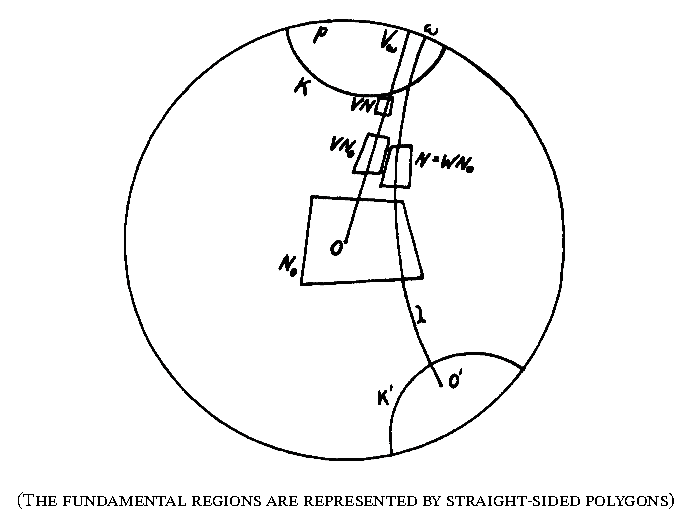
\includegraphics{chap10-vend-scan-01.eps}
\end{figure}

\noindent To simplify notation, we shall denote both $\iota$ (from $X$
to $M_{X}/\sigma$) and the natural map $\sigma^{\natural}$
(from $M_{X}$ to $M_{X}/\sigma$) as $\sigma$. Moreover, for
any $B=\{i_{1}, i_{2},\ldots, i_{m}\} \subset\{1,2,\ldots,
n\}$,~let
\[
e_{B}=e_{i_{1}}e_{i_{2}}\cdots e_{i_{m}},\quad e_{\emptyset}=1,
\]
and then note that $e_{B}$ is well-defined since idempotents in
$M_{X}/\sigma$ commute. Also define the composition $\sigma :
M_{X}\rightarrow M_{X}/\sigma$ followed by $\psi$ as the ``hat''
map $\ \widehat{} =\sigma\circ\psi$, i.e.,
$\widehat{w}=(w\sigma)\psi$. So when $t$ is a product of elements
of $\{s_{1},\ldots, s_{n-2}\}$, then
$\widehat{te}_{B}=(te_{B})\sigma\psi=(t)\sigma\psi(e_{B})\sigma\psi=\widehat{t}\widehat{e}_{B}$.

\begin{lemma}\label{lem10.48.1}
Let $t_{ijk}\in M_{X}$ be such that $\widehat{t}_{ijk}=(i, j,
k)\in A_{n}$ is a $3$-cycle. Then $t_{ijk}e_{i}e_{j}e_{k}
=e_{i}e_{j}e_{k}$ $(mod\ \sigma)$.
\end{lemma}

\begin{proof}Certainly each of $\widehat{s}_{1}=(1,2,3)$ and
$\widehat{s}_{1}^{-1}=(1,3,2)$ is conjugate within the symmetric
group $S_{n}$ to $\widehat{t}_{ijk}=(i,j, k)$. If
$\sigma^{-1}\widehat{s}_{1}\sigma=(i, j, k)$, where $\sigma$ is
odd, then
\[
((2,3)\sigma)^{-1}\widehat{s}_{1}^{-1}((2,3)\sigma)=(i,j, k),
\]
and $(2,3)\sigma$ is even. Thus, there exists $w\in M_{X}$ with $
w\sigma\in\langle\{s_{i}\sigma\}\rangle$ and $\widehat{w}\in
A_{n}$ such that either
\[
\widehat{w}^{-1}\widehat{s}_{1}\widehat{w}=\widehat{t}_{ijk}\quad \mathrm{or}\quad \widehat{w}^{-1}
\widehat{s}_{1}^{-1}\widehat{w}=\widehat{t}_{ijk}.
\]
Second, recall from the group theory case that $\psi$ restricted
to $\langle\{s_{i}\sigma\}\rangle$ is an isomorphism onto
$A_{n}\subset A_{n}^{c}$. It then follows that either
\[
w^{-1}s_{1}w=t_{ijk}\ (\mathrm{mod}\ \sigma)\quad \mathrm{or}\quad w^{-1}s_{1}^{-1}w=t_{ijk}\ (\mathrm{mod}\ \sigma).
\]
(We shall assume the former $\sigma$-equivalence since the other
case is similar). Third, we show that for each $m\in\{1,2,3\}$,
\begin{equation}\label{eq10.48.2}
 w^{-1}e_{m}w=e_{m\widehat{w}}\ (\mathrm{mod}\ \sigma).
\end{equation}
To verify (\ref{eq10.48.2}), apply (4) of 47.2 --- ``move $e_{m}$
to the right,'' i.e.,
\[
w^{-1}e_{m}w=ze_{\ell}\ (\mathrm{mod}\ \sigma),
\]
where $\widehat{z}\in A_{n}$. From this we deduce that
$\widehat{w}^{-1}\widehat{e}_{m}\widehat{w}=\widehat{z}\widehat{e}_{\ell}$.
On the other hand, it is clear that
$\widehat{w}^{-1}\widehat{e}_{m}\widehat{w}=\widehat{e}_{m\widehat{w}}$,
and so $\widehat{z}\widehat{e}_{\ell}=\widehat{e}_{m\widehat{w}}$.
A comparison of the images of these two maps then gives
$\ell=m\widehat{w}$, and it then follows that $i\widehat{z}=i$
except possibly for $i=m\widehat{w}$. Since $\widehat{z}$ is a
permutation, we must have $\widehat{z}=1$. Since the restriction
of $\psi$ to $\langle\{s_{i}\sigma\}\rangle$ is an isomorphism,
$z=1\ (\mathrm{mod}\ \sigma)$, and (\ref{eq10.48.2}) now follows.
From (\ref{eq10.48.2}) and
$w\sigma\in\langle\{s_{i}\sigma\}\rangle$, we have
$w^{-1}e_{1}e_{2}e_{3}w= e_{i}e_{j}e_{k}\ (\mathrm{mod}\ \sigma)$.
We can now calculate that $(w^{-1}s_{1}w)(w^{-1}e_{1}e_{2}e_{3}w)=
t_{ijk}e_{i}e_{j}e_{k}\ (\mathrm{mod}\ \sigma)$. And from this and
(5) of 47.2, we are finished.
\end{proof}

\begin{lemma}\label{lem10.48.3}
Let $t$ and $t_{0}$ be products of elements in $\{s_{1},\ldots,
s_{n-2}\}$. Then
$\widehat{t}\widehat{e}_{B}=\widehat{t}_{0}\widehat{e}_{B}$
implies $(te_{B}, t_{0}e_{B})\in\sigma$.
\end{lemma}

\begin{proof} Let $p_{m}$ be the statement:
\[
p_{m} \equiv\widehat{t}\widehat{e}_{B}=\widehat{t}_{0}\widehat{e}_{B}\quad
\mathrm{when}\quad |B|\leq m\ \Rightarrow\ (te_{B}, t_{0}e_{B})\in\sigma.
\]
We show $p_{0}$, $p_{1}$, $p_{2}$ and (the implication)
``$p_{m-1}\Rightarrow p_{m}$'' are true. If $m= 0$, then
$B=\emptyset$ and $(t,t_{0})\in\sigma$ since, from group theory
[10, p. 298], the homomorphism $\psi$ carries the
subgroup $\langle\{s_{i}\sigma\}\rangle$ of $M_{X}/\sigma$
isomorphically onto the (alternating) subgroup $A_{n}$ of
$A_{n}^{c}$. If $m=1$, then both charts
$\widehat{t}\widehat{e}_{i}$ and $\widehat{t}_{0}\widehat{e}_{i}$
have rank $n-1$ and are one-one. It follows that
$\widehat{t}=\widehat{t}_{0}$, and again from the group theory,
$(t, t_{0})\in\sigma$. Hence, $(te_{i}, t_{0}e_{i})\in\sigma$. If
$m=2$, then
\[
\widehat{t}\widehat{e}_{i}\widehat{e}_{j}=\widehat{t}_{0}\widehat{e}_{i}\widehat{e}_{j}
\]
where the indices $i,j\not\in
\mathbf{r}(\widehat{t}\widehat{e}_{i}\widehat{e}_{j})=\mathbf{r}(\widehat{t}_{0}\widehat{e}_{i}\widehat{e}_{j})$.
In this case we have $B=\{i,j\}$, and we need to show $(te_{B},
t_{0}e_{B})\in\sigma$. Again, it suffices to show that
$\widehat{t}=\widehat{t_{0}}$. And to see that these \emph{even}
permutations are equal, we first pick an even permutation
$\alpha\in A_{n}$ such~that
\[
\widehat{t}\alpha=\widehat{t}_{0}.
\]
Second, we show that $\alpha$ is the identity permutation: For
$k\in N=\{1,2,\ldots, n\}$, if $k\widehat{t}\not\in B$, then
$k\widehat{t}_{0}\not\in B$ and
$k\widehat{t}\alpha=k\widehat{t}_{0}=k\widehat{t}$, showing that
$\alpha$ fixes each member of $N-B$. So $\alpha=1$ or
$\alpha=(ij)$. Since $\alpha$ is even, it cannot be the
transposition $(ij)$. Thus, $\widehat{t}=\widehat{t}_{0}$.

Next suppose $m=|B|\geq 3$, that $p_{m-1}$ is true, and that
$\beta=\widehat{t}\widehat{e}_{B}=\widehat{t}_{0}\widehat{e}_{B}$.
If, for every $l\in\{1,2,\ldots, n\}\
k\widehat{t}=x\widehat{t}_{0}$ then, again by the group theory
case, we are finished. Otherwise, there is an $l\not\in
\mathbf{d}(\beta)$ such~that
\begin{equation}\label{eq10.48.4}
 j=l\widehat{t}\neq l\widehat{t}_{0}=i\quad \mathrm{and}\quad i,j \in B.
\end{equation}
Since $|B|\geq 3$, we have the representation
$\beta=\widehat{t}\widehat{e}_{B}=\widehat{t}\widehat{e}_{i}\widehat{e}_{j}\widehat{e}_{k}
\widehat{e}_{L}=\widehat{t}_{0}\widehat{e}_{i}\widehat{e}_{j}\widehat{e}_{k}\widehat{e}_{L}
=\widehat{t}_{0}\widehat{e}_{B}$, where $B=L\cup\{i, j, k\},
L\cap\{i, j, k\}=\emptyset$, and (\ref{eq10.48.4}) holds. Now let
$\widehat{t}_{ijk}=(i,j,k)$, and apply 48.1 to obtain
\[
t_{0}e_{B}=t_{0}e_{i}e_{j}e_{k}e_{L}=t_{0}t_{ijk}e_{i}e_{j}e_{k}e_{L}\quad (\mathrm{mod}\ \sigma).
\]
It follows that
\[
t_{\ast}=t_{0}t_{ijk}\quad \Rightarrow\quad t_{0}e_{B}=t_{\ast}e_{B}\enspace (\mathrm{mod}\ \sigma).
\]
We now observe that $\widehat{t}$ agrees with $\widehat{t}_{\ast}$
on $\mathbf{d}(\widehat{t}\widehat{e}_{B})\cup\{x\}$. Thus, if
$C=B-\{j\}$, we then~have
\[
\widehat{t}\widehat{e}_{C}=\widehat{t}_{\ast}\widehat{e}_{C}
\]
where $|C|=m-1$. Hence, by the inductive hypothesis, $(te_{C},
t_{\ast}e_{C})\in\sigma$, showing~that
\[
(te_{C}e_{j}, t_{\ast}e_{C}e_{j})=(te_{B}, t_{\ast}e_{B})\in\sigma.
\]
Since $t_{0}e_{B}=t_{\ast}e_{B}\ (\mathrm{mod}\ \sigma)$ we are
finished.
\end{proof}

\begin{theorem}\label{thm10.48.5}
Let $n\geq 3$, and let $M_{X}$ be the free inverse monoid
generated by the set $X=\{s_{1},\ldots, s_{n-2}, e\}$. Let
$\sigma$ be the congruence on $M_{X}$ generated by the following
relations
\begin{align*}
s_{1}^{3} &=(s_{i})^{2}=(s_{i-1}s_{i})^{3}=(s_{j}s_{k})^{2}=1,\quad  \text{for}\quad i>1,\ |j-k|>1, \\
e^{2}&=e, (es_{1})^{3}= (es_1)^{4},\qquad\qquad\qquad\enspace \text{and} \\
(es_{j})^{2}&=(es_{j})^{4}, es_{i}=s_{i}s_{1}^{-1}es_{1},\qquad\qquad\quad \text{for}\quad j>1, i\geq 1.
\end{align*}
Then $M_{X}/\sigma$ is isomorphic to $A_{n}^{c}$.
\end{theorem}

\begin{proof} From 47.2, we may assume that every $w\in M_{X}$ is in a
$\sigma$-class with a word of the form $te_{B}$. So, to assume
that $\psi$ is not one-one is to contradict 48.3. We conclude
that the epimorphism $\psi$ is also a monomorphism.
\end{proof}

\section{Comments}\label{sec10.49}

Our approach to constructing defining relations for $A_{n}^{c}$
runs parallel to that of $C_{n}$ (Chapter~\ref{chap9}). The common
elements indicate a general method for finding presentations of
certain inverse semigroups. To be more precise, let $G\subset
S_{n}$ be a permutation group with presentation $\langle X \mid
\Delta\rangle$, and consider the inverse semigroup
$S=\{\alpha\in C_{n}\mid \alpha$ is a restriction of some
$\gamma\in G$\}. Then what can be said about adding generators
$(e^{2}=e)$ to obtain a presentation of the semigroup~$S$?

In both of the $A_{n}^{c}$ and $C_{n}$ cases, generators
$x_{1},\ldots, x_{k}$ in the group presentation were first
identified with permutations in cycle notation. These generators
were then augmented with an idempotent generator $e=e^{2}$, which
would ultimately correspond to the chart $\varepsilon
=(1](2)\cdots(n)$. Then, using the fact that all idempotents of
rank $n-1$ are conjugate, we ``mechanically generated'' new
relations (between $e$ and the $x_{i}$) by inspecting the path
structure resulting from various multiplications of the charts
corresponding to $x_{1},\ldots, x_{k}, e$.

How do we know which relations to incorporate? Examples in the
$A_{n}^{c}$ case illustrate one answer. Consider the relations
$(es_{1})^{3}=(es_{1})^{4}$ and $(es_{j})^{2}= (es_{j})^{4}$, $j>1$.
We calculate in path notation that $es_{1}$ must correspond to the
chart with path~form
\[
(1](2)\cdots (n)\circ(1,2,3)=(2,3,1](4)\cdots(n).
\]
Such a chart yields a cyclic semigroup of index 3 and period 1
(6.2). That is, the period 1 yields the exponent 4 on
$(es_{1})^{4}$. In contrast, the chart that corresponds to
$es_{j}$, where $j>1$, has path structure
\[
(1] (2)\cdots (n) \circ (1,2)(j+1, j+2)=(2,1](j+1,
j+2)(k_{1})\cdots(k_{n-4}).
\]
In this case, we have a cyclic semigroup of index 2 and period 2,
showing why we have equality $(es_{j})^{2}=(es_{j})^{2+2}$ when
$j>1$. The idea is to pick those relations that show how the
idempotent generator $e$ ``interacts'' with each generator $x\in X$.

Having expanded the generating set $X$ to $X\cup\{e\}$, and the
set of relations $\Delta$ to a set
$\Delta\cup\Delta_{1}$, we then encountered the word problem
--- we needed to establish that the unique morphism $\psi$ was
one-one. To do this, a technical lemma was needed to obtain
canonical forms for words, and an inductive lemma was also needed
to make use of the group presentation as the initial case in an
inductive argument. (Proposition~\ref{prop9.42.11} played a key
role in allowing for the use of the group presentation.)

The presentation of $A_{n}$ used in this chapter was first
introduced by Moore [\ref{bib53}] and later
discussed in Burnside [\ref{bib6}]. The
presentation of $A_{n}^{c}$ first appeared in a paper written by
the author [\ref{bib71e}] and communicated by J.
M. Howie.\index{Howie, J. M.} During the review of that paper,
Howie made several comments that led to a considerably improved
proof of Lemma~\ref{lem10.48.1}.

\chapter{Decomposing Partial Transformations}\label{chap11}

Path notation for charts (partial one-one transformations) is an
extension of cycle notation for permutations. By allowing for the
use of a right bracket ``]'', in conjunction with the usual
parentheses ``('' ``)'', path notation provides to charts what
cycle notation provides to permutations. Here we take the next
step, i.e., by allowing for the use of yet another symbol
``$\rangle$'', path notation is extended to partial
transformations. In particular, partial transformations are
decomposed into circuits and proper paths. The representation is
then used to study idempotents, nilpotents, and cyclic semigroups.

\setcounter{section}{49}

\section{Semigroup Hierarchy}\label{sec11.50}

The \emph{semigroup} $PT_{n}$ \emph{of partial transformations on}
$N=\{1,2,\ldots, n\}$ is the set of all functions $\alpha :
\mathbf{d}\alpha\rightarrow \mathbf{r}\alpha$ that have domain
$\mathbf{d}\alpha\subset N$ and range $\mathbf{r}\alpha\subset N$
under composition. Relative to $S_{n}$ and $C_{n}$, the useful
semigroup hierarchy is
\[
S_{n}\subset C_{n}\subset PT_{n}\subset B_{n},
\]
where $B_{n}$ is the semigroup of all binary relations
$\alpha\subset N\times N$ under composition. In extending path
notation from $C_{n}$ to $PT_{n}$, we shall introduce the right
angle ``$\rangle$'' notation, a notation that identifies those
points where certain proper paths meet a circuit. Examples are
provided in Figure~\ref{fig11.50.1}, where members of $PT_{n}$ are
pictured geometrically.

\begin{figure}[!h]
\includegraphics{chap11-vend-scan-01.eps}
\caption{Partial transformations and path notation.}\label{fig11.50.1}
\end{figure}

\section{Path Notation for Partial Transformations}\label{sec11.51}

Since $S_{n}\subset C_{n}\subset PT_{n}\subset B_{n}$, it is
natural to extend the idea of ``join in $C_{n}$'' to \emph{join}
in $B_{n}$: For $\alpha,\beta\in B_{n}$, define the \emph{join}
$\alpha\beta$ as the union $\alpha\cup\beta$. In particular,
\[
\alpha\beta\in\begin{cases}
C_{n} & \mathrm{if}\ \alpha,\beta\in C_{n}\ \mathrm{and}\ (\mathbf{d}\alpha\cup \mathbf{r}\alpha)\cap(\mathbf{d}\beta\cup \mathbf{r}\beta)=\emptyset\\
PT_{n} & \mathrm{if}\ \alpha,\beta\in PT_{n}\ \mathrm{and}\ x\in \mathbf{d}\alpha\cap
\mathbf{d}\beta\Rightarrow x\alpha=x\beta.
\end{cases}
\]
With this join operation, we could start with proper paths and
circuits in $C_{n}$ and then build partial transformations. We
begin in reverse, however, starting with $\alpha\in
PT_{n}$\index{in $\alpha\in PT_{n}$}\index{path!in $\alpha\in
PT_{n}$} and then defining certain paths induced by $\alpha$.
First, for each $x\not\in \mathbf{d}\alpha\cup \mathbf{r}\alpha$,
we shall call the expression ``$(x]$'' a \emph{maximal proper path
in}\index{path!maximal proper} $\alpha$. And then for $x\in
\mathbf{d}\alpha$ and $k\geq 1$, we let $\eta_{x}=(x,
x\alpha,\ldots, x\alpha^{k}]$ when the set $\{x,
x\alpha,x\alpha^{2},\ldots, x\alpha^{k}\}$ has size $k+1$; and
$\gamma_{x}=(x, x\alpha,\ldots, x\alpha^{k-1})$ when $\{x,
x\alpha,\ldots, x\alpha^{k-1}, x\alpha^{k}\}$ has size $k$ and
$x\alpha^{k}=x$. We call $\eta_{x}$ a \emph{proper path in}
$\alpha$, and $\gamma_{x}$ (whenever it exists) a \emph{circuit
in} $\alpha$. Such a proper path $\eta_{x}$ is also \emph{maximal}
if its left endpoint $ x\in \mathbf{d}\alpha-\mathbf{r}\alpha$ and
its right endpoint $ x\alpha^{k}\in
\mathbf{r}\alpha-\mathbf{d}\alpha$. So maximal proper paths in
$\alpha$ come in two varieties --- those of the $\eta_{x}$ kind
and those expressions ``$(x]$'' where we have $x\not\in
\mathbf{d}\alpha\cup \mathbf{r}\alpha$.

For paths $\eta$ and $\gamma$ in $\alpha$, we say that $\eta$
\emph{meets} $\gamma$ whenever they are not disjoint (as charts).
In particular, if $(\mathbf{d}\eta\ \cup
\mathbf{r}\eta)\cap(\mathbf{d}\gamma \cup
\mathbf{r}\gamma)=\{y\}$, then $\eta$ \emph{meets} $\gamma$ at
$y$; and if both $\eta$ and $\gamma$ are proper paths with a
common proper terminal segment $\sigma$, we say that $\eta$
\emph{meets} $\gamma$ \emph{in} $\sigma$. To illustrate these
concepts, consider the partial transformation
\[
\alpha=\left(\begin{matrix}
1 & 2 & 3 & 4 & 5 & 6 & 7\\
2 & 1 & 1 & 3 & 3 & 7 & -
\end{matrix}\right)\in PT_{7}
\]
as pictured in Figure~\ref{fig11.51.1}. Note that each of
$\eta=(431]$, $\eta'=(531]$, and $\eta''=(67]$ is a proper path in
$\alpha$, but that only $\eta''$ is maximal. Moreover, observe
that $\gamma=(12)$ is a circuit in $\alpha$, that both $\eta$ and
$\eta'$ meet $\gamma$ at 1, and that $\eta$ meets $\eta'$ in the
common terminal segment $\sigma=(31]$.

\begin{figure}[!h]
\includegraphics{chap11-vend-scan-02.eps}
\caption{Maximal proper paths, circuits, and terminal
segments.}\label{fig11.51.1}
\end{figure}

\setcounter{equation}{1}
\begin{lemma}\label{lem11.51.2}
Let $\alpha\in PT_{n}$. Let $\eta$ and $\eta'$ be maximal proper
paths in $\alpha$, and let $\gamma$ and $\gamma'$ be circuits in
$\alpha$. Then the following statements are true:
\begin{enumerate}
\item[(1)] If $\eta$ meets $\eta'$, then either $\eta=\eta'$ or $\eta$ meets $\eta'$ in a
common proper terminal segment.

\item[(2)] Either $\gamma=\gamma'$ or $\gamma$ does not
meet~$\gamma'$.

\item[(3)] For each $y\in \mathbf{r}\alpha-\mathbf{d}\alpha$
there exist $x\in \mathbf{d}\alpha-\mathbf{r}\alpha$ and
$k\geq 1$ such that $x\alpha^{k}=y$, i.e., a maximal
$\eta_{x}=(x, x\alpha,\ldots, x\alpha^{k}=y]$ exists whenever
$y\in \mathbf{r}\alpha - \mathbf{d}\alpha$.
\end{enumerate}
\end{lemma}

\begin{proof} Statements (1) and (2) follow since $\alpha :
\mathbf{d}\alpha\rightarrow \mathbf{r}\alpha$ is a function. For
(3), we use induction: Since $y\in
\mathbf{r}\alpha-\mathbf{d}\alpha$, there exists $x_{1}\in
\mathbf{d}\alpha$ such that $x_{1}\alpha=y$ and $\{x_{1}, y\}$ has
size two. If $x_{1}\not\in \mathbf{r}\alpha$, then, letting
$x=x_{1}$ and $k=1$, we see that $\eta_{x}=(x_{1}, y]=(x,
x\alpha^{1}=y]$ is maximal. Otherwise, there exists $ x_{2}\in
\mathbf{d}\alpha$ such that $x_{2}\alpha=x_{1}$ and $\{x_{2},
x_{1},y\}$ has size three. If $ x_{2}\not\in \mathbf{r}\alpha$,
then, letting $x=x_{2}$ and $k=2$, we see that $\eta_{x}=(x_{2},
x_{1}, y]=(x, x\alpha^{1}, x\alpha^{2}=y]$ is maximal. But
construction (by induction) of such sets $\{x_{k}, x_{k-1},\ldots,
x_{1}, y\}$ must terminate since $N$ is finite. It follows that
the desired $x$ and $k$ exist.
\end{proof}

\begin{theorem}[Unique Representation of Partial Transformations]\label{thm11.51.3}
Every transformation $\alpha\in PT_{n}-\{0\}$ is a join
$\eta_{1}\cdots\eta_{u}\gamma_{1}\cdots\gamma_{v}$ of some
(possibly none) length $\geq 2$ proper paths $\eta_{1},\ldots,
\eta_{u}$ and some (possibly none) circuits $\gamma_{1},\ldots,
\gamma_{v}$ such that for indices $i,j$ $($distinct in $(1)$ and $(2))$:
\begin{enumerate}
\item[(1)] $\eta_{i}$ meets $\eta_{j}$, if at all, in a
common proper terminal segment;

\item[(2)] $\gamma_{i}$ does not meet $\gamma_{j}$; and

\item[(3)] $\eta_{i}$ meets $\gamma_{j}$, if at all, at the
right endpoint of~$\eta_{i}$.
\end{enumerate}
Moreover, this factorization is unique except for the order in
which the paths are written.
\end{theorem}

\begin{proof}Suppose $\alpha\in PT_{n}-\{0\}$. First, if
$|\mathbf{d}\alpha-\mathbf{r}\alpha|=0$, then $\alpha$ is a
permutation of $\mathbf{d}\alpha$ and, consequently, a join of
disjoint circuits $\gamma_{1}\cdots\gamma_{v}$. Next, without loss
of generality, suppose
$\mathbf{d}\alpha-\mathbf{r}\alpha=\{1,2,\ldots, u\}$. Pick $ x\in
\mathbf{d}\alpha-\mathbf{r}\alpha$ and iterate, as far as
possible, to obtain the set $X=\{x, x\alpha,x\alpha^{2},
\ldots\}$. Since $X\subset N$ is finite, there exists a minimum
$k\geq 1$ such that either $ x\alpha^{k}\not\in \mathbf{d}\alpha$
or $x\alpha^{k}=x\alpha^{m}$ for minimum $m>k$. In either case,
define the proper path $\eta_{x}=(x,  x\alpha,\ldots,
x\alpha^{k}]$. And in the case where the minimum $m>k$ exists,
also define the circuit $\gamma_{x}= (x\alpha^{k},\ldots,
x\alpha^{m-1})$. Supposing, again without loss of generality, that
it is precisely when $x\in\{1,2,\ldots, w\}\subset\{1,2,\ldots,
u\}$ that we obtain circuits $\gamma_{x}$, we define
$\beta=\eta_{1}\eta_{2}\cdots\eta_{u}\gamma_{1}\cdots\gamma_{w}$.
That these proper paths and circuits satisfy $(1)-(3)$ follows
from the definition of $\beta$ and $(1)-(2)$ of \ref{lem11.51.2}.
Therefore, if $\alpha=\beta$ we are finished. Otherwise, we shall
show that a join of circuits
$\alpha'=\gamma_{w+1}\cdots\gamma_{v}$ exists such that
$\alpha=\beta\alpha'$: First, define
\[
\alpha'=\alpha|_{\mathbf{d}\alpha-\mathbf{d}\beta}
\]
as the restriction of $\alpha$ to
$\mathbf{d}\alpha-\mathbf{d}\beta$. To see that $\alpha'$ is a
permutation, we shall need several properties:
\begin{enumerate}
\item[(i)] $\mathbf{r}\alpha-\mathbf{d}\alpha=\mathbf{r}\beta-\mathbf{d}\beta$\quad
(Using (3) of \ref{lem11.51.2}, we have $y\in
\mathbf{r}\alpha-\mathbf{d}\alpha\Leftrightarrow$ maximal
$\eta_{x}=(x,\ldots, y]$ exists for some $x\in
\mathbf{d}\alpha-\mathbf{r}\alpha\Leftrightarrow y\in
\mathbf{r}\beta-\mathbf{d}\beta.$)

\item[(ii)] $\mathbf{d}\beta-\mathbf{r}\beta=\mathbf{d}\alpha-\mathbf{r}\alpha$\quad
(Both equal $\{1, 2, \ldots u\}.$)

\item[(iii)] $\mathbf{r}\alpha'\cup \mathbf{r}\beta=\mathbf{r}\alpha$.
\end{enumerate}
We can now show that $\mathbf{d}\alpha'\subset \mathbf{r}\alpha'$,
implying that $\alpha'$ is a permutation of its domain
$\mathbf{d}\alpha'$. Let $y\in \mathbf{d}\alpha'$. Then $ y\in
\mathbf{d}\alpha$ implies $y\not\in
\mathbf{r}\alpha-\mathbf{d}\alpha$. Coupling this with $ y\not\in
\mathbf{d}\beta$ and (i), we deduce
\begin{enumerate}
\item[(iv)] $y\not\in \mathbf{r}\beta$.
\end{enumerate}
Similarly, from $ y\not\in \mathbf{d}\beta-\mathbf{r}\beta$ and
$y\in \mathbf{d}\alpha$, (ii) shows
\begin{enumerate}
\item[(v)] $y\in \mathbf{r}\alpha$.
\end{enumerate}
Then from (iv) and (v), property (iii) yields $y\in
\mathbf{r}\alpha'$, which finishes the proof that $\alpha'$ is a
permutation. Thus as promised,
$\alpha'=\gamma_{w+1}\cdots\gamma_{v}$ is a join of disjoint
circuits. Lastly, to see that the paths in the factorization
$\alpha=\beta\alpha'=\eta_{1}\cdots\eta_{u}\gamma_{1}\cdots\gamma_{v}$
satisfy $(1)-(3)$, it suffices to observe that
$\mathbf{r}\beta\cap \mathbf{r}\alpha'=\emptyset$. (Otherwise, $z
\in \mathbf{r}\beta\cap \mathbf{r}\alpha'=\mathbf{r}\beta\cap
\mathbf{d}\alpha'\subset \mathbf{r}\beta-\mathbf{d}\beta$, showing
$z$ in the right side of (i) and contradicting the fact that $z$
cannot be in the left side of (i) --- $z \in \mathbf{d}\alpha'$
implies $z\in \mathbf{d}\alpha.$)

Turning to uniqueness, we suppose that
$\alpha=\eta_{1}\cdots\eta_{u}\gamma_{1}\cdots\gamma_{v}=\eta_{1}'\cdots
\eta_{w}'\gamma_{1}'\cdots \gamma_{x}'$ has two such
factorizations. If $u=0$, then $\alpha=\gamma_{1}\cdots\gamma_{v}=
\gamma_{1}'\cdots\gamma_{x}'$ is join of circuits and the
uniqueness follows from \ref{lem11.51.2}. So suppose $u\geq 1$. We
claim that $u=w$: First, for any proper path $\eta$ of length
$\geq 2$ we have $\eta=(1,2,\ldots, k]\Rightarrow\{1\}
=\mathbf{d}\eta-\mathbf{r}\eta$. Therefore, (1) and (3) (applied
to $\eta_{1}\cdots\eta_{u})$ imply
$\mathbf{d}\alpha-\mathbf{r}\alpha$ has $u$ elements and $($to
$\eta_{1}'\cdots\eta_{w}')\ w$ elements, i.e., $u=w$. So, by
rearrangement if necessary, for each $i$, we may assume that $i=$
(left endpoint of $\eta_{i}$) $=$ (left endpoint of $\eta_{i}'$).
Next, we make the observation that for any proper path $\eta$ in
any such decomposition of $\alpha$, we have ($\eta$ meets no
circuit in $\alpha$)\quad $\Leftrightarrow$\quad ($\eta$ is maximal in
$\alpha$). An application of this general fact and agreement at
left endpoints (of $\eta_{i}$ and $\eta_{i}'$) show that we have
only two cases:
\begin{enumerate}
\item[(vi)] The right endpoints of both $\eta_{i}$ and $\eta_{i}'$ are in
$\mathbf{r}\alpha-\mathbf{d}\alpha$.

\item[(vii)] There exists a circuit $\gamma$ in $\alpha$ such that both
$\eta_{i}$ and $\eta_{i}'$ meet $\gamma$ at their right endpoints.
\end{enumerate}
In either case, $\eta_{i}$ and $\eta_{i}'$ must also have the same
right endpoint, yielding $\eta_{i}=\eta_{i}'$. It therefore only
remains to show that we may ``cancel'' the proper paths, i.e.,
show that $\gamma_{1}\cdots\gamma_{v}=\gamma_{1}'\cdots\gamma_{x}'$, which
is case $u=0$. To this end, assume that for some index $i, y\in
\mathbf{d}\gamma_{i}$. Then $y\not\in
\mathbf{d}(\eta_{1}\cdots\eta_{u})$ by (3). This implies $y\in
\mathbf{d}\gamma_{j}'$ for some index $j$ and, consequently,
$y\gamma_{i}=y\gamma_{j}'$, showing that the function
$\gamma_{1}'\cdots\gamma_{x}'$ is an extension of
$\gamma_{1}\cdots\gamma_{v}$. Using a similar argument, we can
also show the latter is an extension of the former, thereby
finishing the proof of this~theorem.
\end{proof}

\section{Cilia and Cells of Partial Transformations}\label{sec11.52}

From Theorem~\ref{thm11.51.3}, each nonzero $\alpha\in PT_{n}$ is
a~join
\[
\alpha=(a_{11}\cdots a_{1k_{1}}]\cdots(a_{u1}\cdots a_{uk_{u}}]
(b_{11}\cdots b_{1m_{1}})\cdots(b_{v1}\cdots b_{vm_{v}})
\]
of proper paths (of length $\geq 2$) and circuits that satisfy
(1)--(3) in \ref{thm11.51.3}. To this join, then, we may join the
proper 1-paths $(j_{i}]$, $j_{i}\not\in \mathbf{d}\alpha\cup
\mathbf{r}\alpha$, yielding
\[
\alpha=(j_{1}]\cdots(j_{\ell}](a_{11}\cdots
a_{1k_{1}}]\cdots(a_{u1}\cdots a_{uk_{u}}](b_{11}\cdots
b_{1m_{1}})\cdots(b_{v1}\cdots b_{vm_{v}}).
\]
We shall refer to this unique representation as either the
\emph{path decomposition}\index{path!decomposition in $PT_{n}$} or
\emph{join representation} of $\alpha$. In particular,
$\alpha=0\in PT_{n}$ has join representation $(1]\cdots (n]$, even
though the zero transformation $0$ of $PT_{n}$ is excluded
from~\ref{thm11.51.3}.

In the join representation of a partial transformation, proper
paths are of two kinds, namely, those that meet circuits and those
that do not meet circuits. We call each of the former kind a
\emph{cilium}\index{cilium} (plural $=$
\emph{cilia}\index{cilia}). For example,
\[
\alpha=(1,2,\ldots, i, x_{0}](x_{0}, x_{1},\ldots, x_{m-1})\in PT_{n}
\]
is a join of a cilium ($1,2,\cdots, i, x_{0}]$ and a circuit,
which we clearly mark by replacing the right bracket ``]'' with
the right angle ``$\rangle$'', yielding
\[
\alpha=(1,2,\ldots, i, x_{0}\rangle(x_{0}, x_{1},\ldots, x_{m-1}).
\]
We say that $(x_{0}, x_{1},\ldots, x_{m-1})$ is \emph{associated
with} ($1, 2,\ldots, i, x_{0}\rangle$, and that $(1, 2,\ldots, i,
x_{0}\rangle$ is \emph{associated with} $(x_{0}, x_{1},\ldots,
x_{m-1})$. We may, in fact, have any finite number of cilia
$\eta_{1},\ldots, \eta_{k}$ associated with one circuit $\gamma$,
and, in such a case, the join $\eta_{1}\cdots\eta_{k}\gamma$ is
called a \emph{cell}. A typical cell is pictured in
Figure~\ref{fig11.52.1}, where we see the partial transformation
\[
\left(\begin{array}{cccccccccccc}
1 & 2 & 3 & 4 & 5 & 6 & 7 & 8 & 9 & 10 & 11 & 12\\
2 & 3 & - & 3 & 6 & 7 & 8 & 10 & 7 & 8 & 11 & -
\end{array}\right)\in PT_{12},
\]
whose path decomposition is $(1,
2,3](4,3](5,6,7,8\rangle(9,7,8\rangle(8,10)(11)(12]$. It is clear
that this partial transformation has two cells, one with two cilia
and the other with~none.

\begin{figure}[!h]
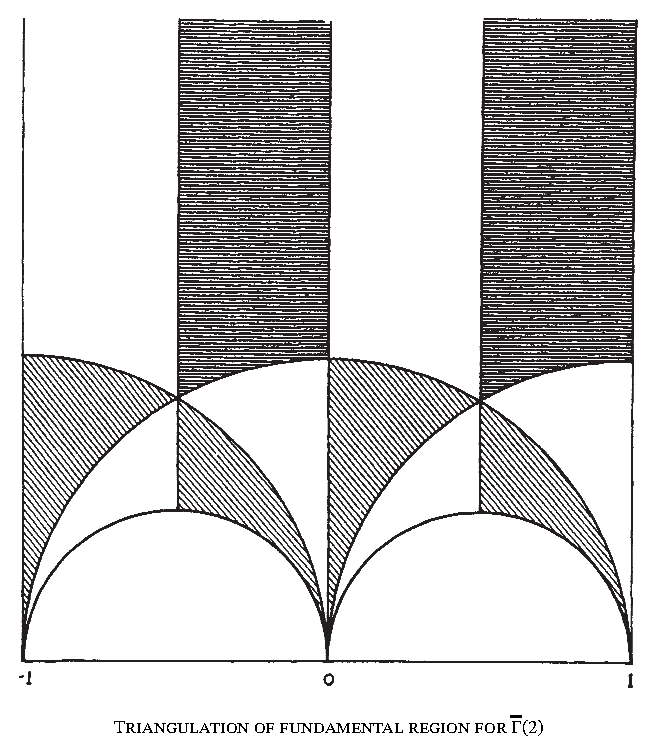
\includegraphics{chap11-vend-scan-03.eps}
\caption{Decomposing a partial transformation.}\label{fig11.52.1}
\end{figure}

\section{Idempotents and Nilpotents}\label{sec11.53}

In this section, we determine the path structure of both
idempotent (\ref{prop11.53.1}) and nilpotent (\ref{prop11.53.2})
partial transformations. (The proof of the nilpotent case is
obvious.)

\begin{proposition}\label{prop11.53.1}
A partial transformation is an idempotent if and only if its path
decomposition is a join of $1$-paths with some (possibly none) cilia
of length~$2$.
\end{proposition}

\begin{proof}Suppose $\varepsilon^{2}=\varepsilon$. If $\varepsilon$ moves $x$ to
$y$, then $\varepsilon$ must fix $y$. In other words, the path
decomposition of $\varepsilon$ must contain the cell
$(xy\rangle(y)$. It follows that $\varepsilon$ is a join of
1-paths with some (possibly none) cilia of length 2. The converse
follows since any cell of the form ($x_{1}, y\rangle \cdots(x_{k},
y\rangle(y)$ is an idempotent.
\end{proof}

\begin{proposition}\label{prop11.53.2}
A partial transformation is nilpotent if and only if its path
decomposition contains no circuits.
\end{proposition}

To illustrate \ref{prop11.53.1} and \ref{prop11.53.2}, consider
$\varepsilon=(4](12\rangle(2)(35\rangle(5)\in PT_{5}$ and
$\eta=(12](3](456](76]\in PT_{7}$.

\section{Multiplication of Partial Transformations}\label{sec11.54}

Learning to multiply partial transformations in path notation is
like learning to multiply charts in path notation, it takes a
little practice. When calculating powers $\alpha^{k}$ of a given
$\alpha\in PT_{n}$, the next two lemmas are helpful. (Their proofs
are straightforward.) In reading these lemmas, keep in mind that
we are using ``$i$'' as a mnemonic for \emph{index}\index{index}.

\begin{lemma}\label{lem11.54.1}
Let $\alpha=(12\cdots ix_{0}\rangle(x_{0}x_{1}\cdots x_{m-1})$,
let $k\geq i$, and let $\ell\in\{1,2,\ldots, i\}$. If we calculate
subscripts modulo $m$, then
\[
\ell\alpha^{k}=\ell\alpha^{i-\ell+1}\alpha^{k-(i-\ell+1)}=x_{0}\alpha^{k-(i-\ell+1)}=x_{k-(i-\ell+1)}.
\]
\end{lemma}

\begin{lemma}\label{lem11.54.2}
Let the path decomposition of $\alpha\in
PT_{n}$\index{idempotent(s)!in $PT_{n}$} be
$\eta_{1}\cdots\eta_{u}\gamma_{1}\cdots\gamma_{v}(\eta_{11}\cdots\eta_{1m_{1}}\gamma_{1}') \cdots
(\eta_{w1}\cdots\eta_{wm_{w}}\gamma_{w}')$ with each $\eta_{j}$ a
proper path, each $\gamma_{j}$ a circuit, and each
$(\eta_{j1}\cdots\eta_{jm_{j}}\gamma_{j}')$ a cell. Then for
each~$k\geq 1$,
\[
\alpha^{k}=\eta_{1}^{k}\cdots\eta_{u}^{k}\gamma_{1}^{k}\cdots\gamma_{v}^{k}
(\eta_{11}\cdots\eta_{1m_{1}}\gamma_{1}')^{k}\cdots(\eta_{w1}\cdots\eta_{wm_{w}}\gamma_{w}')^{k}.
\]
\end{lemma}

\begin{theorem}\label{thm11.54.3}
If $\alpha\in PT_{n}$ has path decomposition $\alpha=(12\cdots
ix_{0}\rangle(x_{0}\cdots x_{m-1})$, then the index of $\alpha$
is~$i$.
\end{theorem}

\begin{proof} From 54.1, for every $k\geq i$, we have $\alpha^{k}=(1,
x_{k-i}\rangle(2,x_{k-(i-1)}\rangle\cdots (i,x_{k-1}\rangle
(x_{0}\cdots x_{m-1})^{k}$. On the other hand, if $k$ is positive
and less than $i$, then for $t= k-r\ (\mathrm{mod}\ m)$ where
$i=qk+r$ and $0\leq r<k$, we have $1\alpha^{k}\in\{2,\ldots, i\}$,
showing that ($1,1\alpha^{k}, 1\alpha^{2k},\ldots, x_{t}\rangle$
is a cilium of length at least 3 appearing in the decomposition of
$\alpha^{k}$. It then follows, since all cilia in the
decompositions of powers of $\alpha$ greater than $i$ have length
2, that the index of $\alpha$ cannot be less than $i$. To see that
the index of $\alpha$ is $i$, note that $\alpha^{i}=(1,
x_{0}\rangle(2, x_{1}\rangle\cdots(i, x_{i-1}\rangle(x_{0}\cdots
x_{m-1})^{i}$ and~that
\[
\alpha^{i}=\alpha^{i+m}=(1, x_{0+m}\rangle(2,x_{1+m}\rangle\cdots
(i, x_{i-1+m}\rangle (x_{0}\cdots x_{m-1})^{i+m},
\]
which finishes the proof.
\end{proof}

\setcounter{equation}{4}
\begin{corollary}\label{cor11.54.5}
Let
$\alpha=\eta_{1}\cdots\eta_{u}\gamma_{1}\cdots\gamma_{v}(\eta_{11}
\cdots\eta_{1m_{1}}\gamma_{1}')\cdots(\eta_{w1}\cdots\eta_{wm_{w}}\gamma_{w}')$
be the decomposition of $\alpha\in PT_{n}$, with each $\eta_{j}$ a
proper path, each $\gamma_{j}$ a circuit, and each
$\eta_{j1}\cdots\eta_{jm_{j}}\gamma_{j}'$ a cell. Then for
$\ell(\eta)= length$~of $\eta$,
\[
\text{index\ of}\ \alpha=\max\{\ell(\eta_{1}),\ldots,
\ell(\eta_{u}), \ell(\eta_{11})-1,\ldots, \ell(\eta_{wm_{w}})-1\},
\]
and the period of $\alpha$ is the least common multiple of the
lengths of the circuits $\gamma_{1},\ldots, \gamma_{v},
\gamma_{1}',\ldots, \gamma_{w}'$. Moreover, if the join
representation of $\alpha$ contains no proper paths (circuits),
then the index (period)\index{partial!index and period of} of
$\alpha$ is~$1$.
\end{corollary}

\begin{proof} Use \ref{thm11.51.3}, \ref{lem11.54.2}, \ref{thm11.54.3}, and the fact that the order of a
permutation is the least common multiple of the lengths of
its~cycles.
\end{proof}

\section{Cyclic Semigroups of Partial Transformations}\label{sec11.55}

Expressing $\alpha\in PT_{n}$ in its join representation, we
``know'' (via \ref{cor11.54.5}) the index and period of
$\langle\alpha\rangle$, i.e., we know $\langle\alpha\rangle$ up to
isomorphism. As a consequence, the isomorphism classes of cyclic
subsemigroups of $PT_{n}$ may be determined by listing all
possible forms of join representations.

\begin{table}[!h]
\caption{Index and Period for $\alpha\in
PT_{4}-C_{4}$.}\label{tab11.55.1}
{\begin{tabular}{|l|c|c|c|c|}
\hline
\textbf{number of} $m\rightarrow k$ \textbf{maps} &\textbf{path structure} &\textbf{number} &\textbf{index} &\textbf{period} \\
\hline
$\big(\kern0.5pt\begin{smallmatrix}4 \\ 2\end{smallmatrix}\kern0.5pt\big)\big(\kern0.5pt\begin{smallmatrix}4\\ 1\end{smallmatrix}\kern0.5pt\big)S(2,1)1!=24$ & (21$\rangle$(1)(3](4] &12 &1 &1 \\
&(13](23](4] &12 &2 &1 \\
\hline
$\big(\kern0.5pt\begin{smallmatrix}4\\ 3\end{smallmatrix}\kern0.5pt\big)\big(\kern0.5pt\begin{smallmatrix}4\\ 1\end{smallmatrix}\kern0.5pt\big)S(3,1)1!=16$ &(21$\rangle$(31$\rangle$(1)(4] &12 &1 &1 \\
&(14](24](34] &4 &2 &1 \\
\hline
$\big(\kern0.5pt\begin{smallmatrix}4\\ 4\end{smallmatrix}\kern0.5pt\big)\big(\kern0.5pt\begin{smallmatrix}4\\ 1\end{smallmatrix}\kern0.5pt\big)S(4,1)1!=4$ &(21$\rangle$(31$\rangle$(41$\rangle$(1) &4 &1 &1 \\
\hline
$\big(\kern0.5pt\begin{smallmatrix}4\\ 3 \end{smallmatrix}\kern0.5pt\big)\big(\kern0.5pt\begin{smallmatrix}4\\ 2\end{smallmatrix}\kern0.5pt\big)S(3,2)2!=144$ &(1)(32$\rangle$(2)(4] &24 &1 &1 \\
&(31$\rangle$(12)(4] &24 &1 &2 \\
&(321$\rangle$(1)(4] &24 &2 &1 \\
&(14](24](3) &12 &2 &1 \\
&(14](234] &24 &2 &1 \\
&(14](23$\rangle$(3) &24 &2 &1 \\
&(124](324] &12 &3 &1 \\
\hline
$\big(\kern0.5pt\begin{smallmatrix}4\\ 4\end{smallmatrix}\kern0.5pt\big)\big(\kern0.5pt\begin{smallmatrix}4\\ 2\end{smallmatrix}\kern0.5pt\big)S(4,2)2!=84$ &(2)(31$\rangle$(41$\rangle$(1) &12 &1 &1 \\
&(21$\rangle$(1)(43$\rangle$(3) &12 &1 &1 \\
&(41$\rangle$(23$\rangle$(31) &12 &1 &2 \\
&(31$\rangle$(41$\rangle$(12) &12 &1 &2 \\
&(321$\rangle$(41$\rangle$(1) &24 &2 &1 \\
&(321$\rangle$(421$\rangle$(1) &12 &2 &1 \\
\hline
$\big(\kern0.5pt\begin{smallmatrix}4\\ 4\end{smallmatrix}\kern0.5pt\big)\big(\kern0.5pt\begin{smallmatrix}4\\ 3\end{smallmatrix}\kern0.5pt\big)S(4,3)3!=144$ &(2)(3)(41$\rangle$(1) &12 &1 &1 \\
&(2)(431$\rangle$(1) &24 &2 &1 \\
&(23)(41$\rangle$(1) &12 &1 &2 \\
&(1)(42$\rangle$(23) &24 &1 &2 \\
&(431$\rangle$(12) &24 &2 &2 \\
&(41$\rangle$(123) &24 &1 &3 \\
&(4321$\rangle$(1) &24 &3 &1 \\
\hline
&\multicolumn{2}{c}{$\textbf{Total} =\qquad\quad\enspace \textbf{416}$} & & \\
\hline
\end{tabular}}{}
\end{table}

A listing of the possible forms of join representations in the
$PT_{4}-C_{4}$ case appears in Table~\ref{tab11.55.1}. (Recall
that the forms for charts in $C_{4}$ appear in
Table~\ref{tab2.7.1}.) The number of members of $PT_{4}$~is
\[
1+\sum\nolimits_{1\leq k\leq m\leq 4}\ \big(\kern0.5pt\begin{smallmatrix}
4\\
m
\end{smallmatrix}\kern0.5pt\big)\big(\kern0.5pt\begin{smallmatrix}
4\\
k
\end{smallmatrix}\kern0.5pt\big)\ S(m, k)k!=625.
\]
In this formula, the Stirling number $S(m, k)$ of the second kind
is the number of partitions of a set of $m$ objects into $k$
classes (see page 40 of Berge [\ref{bib3}]).
Among these 625 members of $PT_{4}$, we~find
\[
1+\textstyle\sum_{m=1}^{4} \big(\kern0.5pt\begin{smallmatrix}
4\\
m
\end{smallmatrix}\kern0.5pt\big)^2 m!=209
\]
charts (partial one-one transformations), i.e., 209 of the 625 are
members of $C_{4}\subset PT_{4}$. Thus, our Table~\ref{tab11.55.1}
displays the index and period of the $625-209=416$ members of
$PT_{4}-C_{4}$.

\section{Comments}\label{sec11.56}

According to Higgins\index{Higgins, P.
M.} [\ref{bib28}, page 70], it was
Suschkewitsch\index{Suschkewitsch, A.K.}
[\ref{bib73b}] who, in 1928, first depicted a
full transformation $\alpha\in T_{n}\subset PT_{n}$ as a digraph
on $n$ vertices in which $ij$ is a diedge whenever $i\alpha=j$.
These digraphs are characterized by the condition that every
vertex have out degree one, in which case they are called
\emph{functional digraphs}. The number of non-isomorphic
functional digraphs having $n$ vertices was determined in 1959 by
Harary\index{Harary, F.} [\ref{bib27}].

Since their introduction, many authors have used functional
digraphs. For example, in 1968 D\'{e}nes
[\ref{bib11a}] illustrated in his Figure 3 the
concept of ``mainpermutation'' of $\alpha\in T_{n}$, which, by
considering $\alpha\in PT_{n}$, is the union of the circuits
appearing in its path decomposition. And in 1988 these digraph
representations (of full transformations) were employed by Higgins
[\ref{bib28a}] in finding algorithms to solve
equations such~as
\[
\alpha x^{m}\beta=\gamma\quad \mathrm{and}\quad \alpha x=x\beta\quad
(\alpha,\beta, \gamma\in T_{n}).
\]

The approach taken in this chapter may be viewed as a variant of
these digraph representations. Indeed, each $\alpha\in PT_{n}$ may
also be pictured as a digraph on $n$ vertices. In this case,
however, the characterizing condition is that every vertex have
out degree at most one. From this view, the path notation applied
here to partial transformations captures the essential features of
the digraph representation. The ideas and results of this chapter
are due to Konieczny\index{Konieczny, J.} and Lipscomb
[\ref{bib37a}].

\chapter{Commuting Partial Transformations}\label{chap12}

Like charts, commuting partial transformations $\alpha
\circ\beta=\beta \circ\alpha$ also determine mappings of initial
segments onto terminal segments and circuits onto circuits. In
addition to circuits and segments, however, the $PT_{n}$ case
involves mappings of cilia. Exactly where a cilium in $\alpha$ may
be mapped depends on whether or not its right-endpoint is in the
domain of $\beta$.

We begin with examples of mappings of cilia, segments, and
circuits (\S\ref{sec12.57}). Following the examples, we approach
commutativity in $PT_{n}$ by first representing $\alpha\in PT_{n}$
as the join
$\alpha=\eta_{1}\cdots\eta_{u}\gamma_{1}\cdots\gamma_{v}$ of its
maximal proper paths $\eta_{i}$ and its cells $\gamma_{j}$
(\S\ref{sec12.58}). Our goal (Theorem~\ref{thm12.58.8}) is that of
showing $\alpha \circ\beta=\beta \circ\alpha$ is equivalent to
($i$) $\beta$ maps some (possibly none) initial segments of the
$\eta_{i}$ onto terminal segments of the $\eta_{i}; (ii)\beta$
maps some (possibly none) of the cells $\gamma_{j}$ onto subcells
of the $\gamma_{j}$; and ($iii$) $\beta$ maps some (possibly none)
proper initial segments of the cilia onto terminal segments of
the~$\eta_{i}$.

An immediate application of this characterization yields the
$C_{n}$ case --- since cells $\gamma_{j}$ with no cilia are
circuits, ($i$) and ($ii$) are the characterizing conditions for
commuting charts. A more subtle application is that of computing
the order $|C(\varepsilon)|$ of the centralizer $C(\varepsilon)$
of an idempotent $\varepsilon\in PT_{n}$ (\S\ref{sec12.59}).

\setcounter{section}{56}
\section{Examples}\label{sec12.57}

Let $\alpha=(123](45\rangle(567)=\eta\gamma$, where the maximal
proper path $\eta=(123]$ and ($45\rangle$ is a cilium; and suppose
that $\alpha$ and $\beta=(1)(2)(43\rangle(3)$ are partial
transformations in $PT_{7}$ (Figure~\ref{fig12.57.1}). Then
$\alpha \circ\beta=(123]=\beta \circ\alpha$, and we see that
$\beta$ maps initial segments onto terminal segments, namely,
$(123]\mapsto(123]$ and ($4]\mapsto(3]$. The former illustrates
condition (\emph{i}) above, while the latter illustrates ($iii$).

To illustrate condition ($ii$), consider
$\alpha=(12](345\rangle(567)=\eta\gamma$, where the cell
$\gamma=(345\}(567)$. Then $\sigma=(45\rangle(567)$ is a subcell
of $\gamma$ and, for the partial transformation
$\beta=(345\rangle(567)$ illustrated in Figure 57.2, we see that
$\beta$ maps $\gamma$ onto $\sigma$ and that $\alpha
\circ\beta=(35)(576)=\beta \circ\alpha$.

\begin{figure}[!h]
\includegraphics{chap12-vend-scan-01.eps}
\caption{Mapping initial segments onto terminal segments.}\label{fig12.57.1}
\end{figure}

\begin{figure}[!h]
\includegraphics{chap12-vend-scan-02.eps}
\caption{Mapping cells onto subcells.}\label{fig12.57.2}
\end{figure}

In the other picture in Figure~\ref{fig12.57.2}, we have
$\alpha=(12\rangle(23)(4567)$ and $\beta= (42](53](62](73]$.
Again, $\beta$ maps a cell (4567) onto a subcell (23) --- (23) is
a subcell of (12$\rangle$(23) --- and, as before, $\alpha
\circ\beta=(43](52](63](72]=\beta \circ\alpha$. This example also
illustrates the phenomenon of ``folding'' a $k$-circuit onto an
$\ell$-circuit $m=2$ times, i.e., $\beta$ folds the 4-circuit
(4567) onto the 2-circuit (23) two times. It is obvious that such
a folding can only occur when $\ell$ divides $k$ (for $m>2$, see
Figure~\ref{fig12.58.4}).

\section{Mapping Initial Segments and Cells}\label{sec12.58}

Recall that a partial transformation $\alpha\in PT_{n}$ may be
expressed as a join
$\alpha=\eta_{1}\cdots\eta_{u}\gamma_{1}\cdots\gamma_{v}$ of
proper paths $\eta_{i}$ (maximal in $\alpha$) and cells
$\gamma_{j}= \eta_{j1}\cdots\eta_{jm_{j}}\gamma_{j}'$, where the
$\eta_{jk}$ are the cilia associated with the circuit
$\gamma_{j}'$. This representation allows us to describe those
$\beta\in PT_{n}$ that commute with $\alpha$ --- it is the action of
$\beta$ on the $\eta_{i}$, the $\eta_{jk}$, and the $\gamma_{j}$
that determines whether $\beta$ commutes with $\alpha$. To deal
with the $\eta_{i}$ and the $\eta_{jk}$, we need to recall that
(the representation) $(i_{1}\cdots i_{k}]$ has
\begin{align*}
\mathrm{initial\ sets}{:}\quad &\{i_{1}\}, \{i_{1}, i_{2}\},\ldots, \{i_{1}, i_{2},\ldots, i_{k}\};\\
\mathrm{terminal\ sets}{:}\quad &\{i_{1}, i_{2},\ldots,i_{k}\}, \ldots, \{i_{k-1}, i_{k}\}, \{i_{k}\};\\
\mathrm{initial\ segments}{:}\quad &(i_{1}], (i_{1}i_{2}],\ldots, (i_{1}\cdots i_{k}];\quad \mathrm{and} \\
\mathrm{terminal\ segments}{:}\quad &(i_{1}\cdots i_{k}],\ldots, (i_{k-1}i_{k}], (i_{k}].
\end{align*}
And for mapping segments onto segments, we extend the idea to
$PT_{n}$. If $\beta$ and the proper path $\eta=(i_{1}\cdots
i_{k}]$ are members of $PT_{n}$, and if there is an index $w$ such
that $\mathbf{d}\beta$ meets $\{i_{1},\ldots, i_{w},\ldots,
i_{k}\}$ in the initial set $\{i_{1},\ldots, i_{w}\}$, then for
any proper path $\eta'=(j_{1}\cdots j_{v}\ell_{1}\cdots
\ell_{w}]\,(v\geq 0)$ such that
$i_{1}\beta=\ell_{1},\ldots,i_{w}\beta=\ell_{w}$, we shall say
that $\beta$ \emph{maps an initial segment of} $\eta$ \emph{onto}
a \emph{terminal segment of}~$\eta'$.

In the following lemma, we consider commuting partial
transformations $\alpha$ and $\beta$. The focus is on how $\beta$
maps proper paths in~$\alpha$.

\begin{lemma}[Mapping initial segments onto terminal
segments]\label{lem12.58.1} Let $\alpha,\beta\in PT_{n}$ be such
that $\alpha \circ\beta=\beta \circ\alpha$, and let $\eta$ be a
proper path $(i_{1}\cdots i_{k}]$ in $\alpha$ such that some
$i_{u}\in \mathbf{d}\beta$. If $\eta$ is maximal in $\alpha$, or
if $\eta$ is a cilium such that $i_{k}\not\in \mathbf{d}\beta$,
then $\beta$ maps an initial segment of $\eta$ onto a terminal
segment of some maximal proper path in~$\alpha$.
\end{lemma}

\begin{proof}Let $x,y\in N=\{1,\ldots, n\}$ and suppose $\delta\in
PT_{n}$. We shall use a diagram
$x\mathop{\rightarrow}\limits^{\delta} y$ to mean that $ x\in
\mathbf{d}\delta$ and $x\delta=y$. The proof is based on the
observation that $\alpha \circ\beta=\beta \circ\alpha$ is
equivalent to the following two conditions:\\

\begin{align}
\label{eq12.58.2}\\[-3pc]
\includegraphics{chap12-vend-scan-03.eps}\notag
\end{align}

\begin{align}
\label{eq12.58.3}\\[-3pc]
\includegraphics{chap12-vend-scan-04.eps}\notag
\end{align}
So suppose $\alpha \circ\beta=\beta \circ\alpha$, i.e., that both
(\ref{eq12.58.2}) and (\ref{eq12.58.3}) hold. Consider first the
case where $\eta=(i_{1}\cdots i_{k}]$ is maximal in $\alpha$. If
$w$ is the largest index such that $ i_{w}\in \mathbf{d}\beta$,
then, by~(\ref{eq12.58.2}),
\begin{figure}[!h]
\includegraphics{chap12-vend-scan-05.eps}
\end{figure}

\noindent By (\ref{eq12.58.3}) and the maximality of $w$, we have
$\ell_{w}\not\in \mathbf{d}\alpha$, implying that $\ell_{w}$ is
the right-endpoint of a maximal proper path $(j_{1}\cdots
j_{v}\ell_{1}\cdots\ell_{w}](v\geq 0)$. It follows that we are
finished with the case where $\eta$ is maximal in $\alpha$. So now
suppose that $\eta=(i_{1}\cdots i_{k}\rangle$ is a cilium in $\alpha$
with $ i_{k}\not\in \mathbf{d}\beta$. Again, letting $w$ be the
largest index such that $ i_{w}\in \mathbf{d}\beta$, we obtain the
diagram above. By (\ref{eq12.58.3}), the maximality of $w$, and
the fact that $ i_{k}\not\in \mathbf{d}\beta$, we have $
\ell_{w}\not\in \mathbf{d}\alpha$. The desired result follows.
\end{proof}

Turning to cells and subcells, we recall that when both $\alpha$
and $\beta$ are charts, then each cell $\gamma$ in $\alpha$ has no
cilia, and that $\alpha \circ\beta=\beta \circ\alpha$ restricts
$\beta$ to mapping $k$-circuits onto $k$-circuits. When $\beta$ is
not a chart, however, $\beta$ may ``fold'' a $k$-circuit onto an
$\ell$-circuit $m$ times $(k=m\ell)$. This folding is depicted in
Figure~\ref{fig12.58.4}, where the arrows are mappings of the unit
circle $S^{1}$ (in the complex plane) onto itself, e.g., the $m=2$
map $S^{1}\rightarrow S^{1}$ given by $z\mapsto z^{2}$.

\setcounter{figure}{3}
\begin{figure}[!h]
\includegraphics{chap12-vend-scan-06.eps}
\caption{Folding a $k$-circuit onto an $\ell$-circuit $m$
times.}\label{fig12.58.4}
\end{figure}

Even when the circuits have associated cilia, we may have
foldings. For instance, by slightly modifying the pictures in
Figure~\ref{fig12.58.4}, we may fold both a cilium and its
associated circuit onto a circuit (Figure~\ref{fig12.58.5}).

\begin{figure}[!h]
\includegraphics{chap12-vend-scan-07.eps}
\caption{Folding both a cilium and its associated circuit onto a circuit.}\label{fig12.58.5}
\end{figure}


To deal with these foldings, for any cell
$\sigma=\eta_{1}\cdots\eta_{k}\sigma'$ with cilia $\eta_{i}$ and
circuit $\sigma'$, we define a \emph{subcell}\index{subcell} of
$\sigma$ to be any partial transformation
$\eta_{1}'\cdots\eta_{k}'\sigma'$ where each $\eta_{i}'$ is a
terminal segment of the corresponding $\eta_{i}$. It follows that
each subcell of $\sigma$, as a partial transformation, is also a
cell; and under inclusion, $\sigma$ and $\sigma'$ are,
respectively, the maximum and minimum subcells of $\sigma$.
Subcells may be pictured as in Figure~\ref{fig12.58.7}, where the
circle representing $\sigma'$ is oriented clockwise, and the edges
that collectively represent the cilia are oriented ``toward the
circle.''

In general, each cell\index{morphism(s)!of cells} corresponds to a
digraph --- one that has one circuit and all of its other
diedges (defined by the cilia) directed toward the circuit. This
digraph view of a cell motivates the following definition, where
the subscript arithmetic is the appropriate modulo arithmetic.

\setcounter{equation}{5}
\begin{definition}[Morphisms\index{morphism(s)} of Cells]\label{defn12.58.6}
Let $\alpha,\beta\in PT_{n}$. Let $\alpha$ have a cell $\gamma$,
with $k$ circuit $\gamma'=(i_{0}\cdots i_{k-1})$, and a cell
$\sigma$, with $\ell$-circuit $\sigma'=(j_{0} \cdots j_{\ell-1})$.
We say that $\beta$ maps $\gamma$ onto a subcell of $\sigma$ if
$\ell$ divides $k$, if $\mathbf{d}\gamma\subset \mathbf{d}\beta$,
if for some $u$, $i_{0}\beta=j_{u}$, $i_{1}\beta=j_{u+1}, \ldots\,$, and
if for every cilium $\eta=(n_{1}\cdots n_{p}\rangle$ in $\gamma$,
exactly one of the following holds: There is a $j_{w}\in
\mathbf{d}\sigma'$ such that $n_{1}\beta=j_{w}$,
$n_{2}\beta=j_{w+1},\ldots\,$; or there is~a terminal segment
$(m_{1}\cdots m_{t}j_{w}\rangle$ of a cilium in $\sigma$ such that
$1\leq t<p$ and
\[
n_{1}\beta=m_{1},\ldots, n_{t}\beta=m_{t},\ n_{t+1}\beta=j_{w},\ n_{t+2}\beta=j_{w+1},\ldots\,.
\]
\end{definition}

If $\gamma$ and $\sigma$ are cells in $\alpha$, and if $\beta$
maps $\gamma$ onto a subcell of $\sigma$, then it follows from
\ref{defn12.58.6} that $\alpha$ restricted to $(\mathbf{d}\gamma)\beta$ is a
subcell of $\sigma$.


\setcounter{figure}{6}
\begin{figure}[!h]
\includegraphics{chap12-vend-scan-08.eps}
\caption{A cell and some of its subcells.}\label{fig12.58.7}
\end{figure}

\setcounter{equation}{7}
\begin{theorem}\label{thm12.58.8}
Let $\alpha,\beta\in PT_{n}$. Then $\alpha \circ\beta=\beta
\circ\alpha$ if and only if
\begin{enumerate}
\item[(\emph{i})] when $\eta=(i_{1}\cdots i_{k}]$ is maximal in
$\alpha$ such that some $i_{u}\in \mathbf{d}\beta$, then
$\beta$ maps an initial segment of $\eta$ onto a terminal
segment of some maximal proper path in~$\alpha$;

\item[(\emph{ii})] when $\gamma$ is a cell in $\alpha$ with circuit
$\gamma'=(i_{0}\cdots i_{k-1})$ such that some $i_{u}\in
\mathbf{d}\beta$, then $\beta$ maps $\gamma$ onto a subcell of
some cell in $\alpha$; and

\item[(\emph{ii})] when $\gamma=\cdots\eta\cdots\gamma'$ is a cell
in $\alpha$ with circuit $\gamma'=(i_{0}\cdots i_{k-1})$ and a
cilium $\eta=(\cdots w\cdots i_{u}\rangle$ such that
$i_{u}\not\in \mathbf{d}\beta$ but $w \in \mathbf{d}\beta$,
then $\beta$ maps an initial segment of $\eta$ onto a terminal
segment of some maximal proper path in~$\alpha$.
\end{enumerate}
\end{theorem}

\begin{proof} Suppose $\alpha \circ\beta=\beta\circ\alpha$. Then ($i$) and
($iii$) follow from \ref{lem12.58.1}. To see that ($ii$) holds, we shall use
\ref{defn12.58.6} and the notation therein. So we already have
$\gamma'=(i_{0}\cdots i_{k-1})$ and some $ i_{u}\in
\mathbf{d}\beta$. Our first observation is that we may assume that
$u=0$. Second, we define $j_{0}=i_{0}\beta$. Coupling this with
the fact that $\gamma'$ is a circuit in $\alpha$, we~have
\begin{figure}[!h]
\includegraphics{chap12-vend-scan-09.eps}
\end{figure}

\noindent which, by (\ref{eq12.58.2}), extends to the commutative diagram
\begin{figure}[!h]
\includegraphics{chap12-vend-scan-10.eps}
\end{figure}

\noindent It follows that $\beta$ folds the $k$-circuit $\gamma'$ onto an
$\ell$-circuit $\sigma'=(j_{0}\cdots j_{\ell-1})$, where $\ell$ is
either the smallest index in $\{1,\ldots, k-1\}$ such that
$j_{\ell}=j_{0}$, or (if no such index exists) $\ell=k$. Moreover,
we see that $\ell$ must divide $k$; and we define $\sigma$ to be the
cell in $\alpha$ that contains $\sigma'$. To see that
$\mathbf{d}\gamma\subset \mathbf{d}\beta$, suppose
$\eta=(n_{1}\cdots n_{p}\rangle$ is associated with $\gamma'$,
then, from the diagram above, there is an index $u$ such that
$n_{p}\beta=j_{u}$. So again, we~have
\begin{figure}[!h]
\includegraphics{chap12-vend-scan-11.eps}
\end{figure}

\noindent which, by (\ref{eq12.58.2}), extends to the commutative diagram\\

\begin{align}\label{eq12.58.9}
\\[-3pc]
\includegraphics{chap12-vend-scan-12.eps}\notag
\end{align}
Thus, $\mathbf{d}\eta\subset \mathbf{d}\beta$, and it follows that
$\mathbf{d}\gamma\subset \mathbf{d}\beta$. So at this point in the
proof, we have $(n_{1}\cdots n_{p}\rangle\,(p>1)$ in $\gamma$ and
need to address the cases $n_{1}\beta\in \mathbf{d}\sigma'$ and
$n_{1}\beta\not\in \mathbf{d}\sigma'$: If $n_{1}\beta\in
\mathbf{d}\sigma'$, then for some index $w$, we have
$n_{1}\beta=j_{w}$, and the diagram (\ref{eq12.58.9}) becomes
\begin{figure}[!h]
\includegraphics{chap12-vend-scan-13.eps}
\end{figure}

\noindent as specified in 58.6. In the other case, $n_{1}\beta\not\in
\mathbf{d}\sigma'$ and we first choose $t$ as~the largest index
such that $n_{t}\beta\not\in \mathbf{d}\sigma'$, which implies
that $n_{t+1}\beta=j_{w}$ for some index $w$. Then the diagram
(\ref{eq12.58.9}) becomes
\begin{figure}[!h]
\includegraphics{chap12-vend-scan-14.eps}
\end{figure}

\noindent as specified in 58.6. It follows, since $m_{t}\not\in
\mathbf{d}\sigma'$, that the desired terminal segment
$(m_{1}\cdots m_{t}j_{w}\rangle$ of a cilium in $\sigma$ exists.
This finishes the proof of (\emph{ii}). To see the converse,
suppose that $\alpha,\beta\in PT_{n}$ satisfy (\emph{i}), (\emph{ii}),
and (\emph{iii}). We shall show that $\alpha \circ\beta=\beta
\circ\alpha$ by showing $\alpha$ and $\beta$ satisfy both (58.2)
and (58.3). For (58.2), we begin with the diagram
\begin{figure}[!h]
\includegraphics{chap12-vend-scan-15.eps}
\end{figure}

\noindent Then $x\in \mathbf{d}\alpha$, which implies that $x$ is either in
a proper path $(\cdots xy\cdots]$ (maximal in $\alpha$) or a cell
in $\alpha$. If $(\cdots xy\cdots]$ is maximal in $\alpha$, then
(\emph{i}) and $ y\in \mathbf{d}\beta$ imply that there is a maximal
proper path $(\cdots x\beta y\beta\cdots]$ in $\alpha$, in which case
we are finished. On the other hand, if $(\cdots xy\cdots)$ is a
circuit in $\alpha$, then apply (\emph{ii}). Finally, if $(\cdots
xy\cdots t\rangle$ is a cilium in $\alpha$, then apply (\emph{ii})
when $ t\in \mathbf{d}\beta$, and (\emph{iii}) when $ t\not\in
\mathbf{d}\beta$. Thus, (\ref{eq12.58.2}) is true. The proof of
(\ref{eq12.58.3}) is~similar.
\end{proof}

\section{Orders of Centralizers of Idempotents}\label{sec12.59}

From 53.1, an idempotent $\varepsilon \in PT_{n}$ is join
$\varepsilon=\eta_{1}\cdots\eta_{m_{0}}\varepsilon_{1}\cdots\varepsilon_{p}$
of proper 1-paths $\eta_{k}$ and cells $\varepsilon_{j}=(l_{j1},
l_{j}\rangle(l_{j2}, l_{j}\rangle\cdots(l_{jm_{j}},
l_{j}\rangle(l_{j})\ (m_{j}\geq 0)$, where the cilia $(l_{jq},
l_{j}\rangle$ (if they exist) are 2-paths. We note that $m_{j}\geq
0$ denotes the number of cilia in $\varepsilon_{j}$, and, in
particular, if $m_{j}=0$, then $\varepsilon_{j}=(l_{j})$ is a
1-circuit. We also observe that $m_{0}+m_{1}+\cdots+m_{p}$ counts
the number of proper paths in the path decomposition
of~$\varepsilon$.

\begin{proposition}\label{prop12.59.1}
Let $\varepsilon
=\eta_{1}\cdots\eta_{m_{0}}\varepsilon_{1}\cdots\varepsilon_{p}$
be the join representation of an idempotent $\varepsilon \in
PT_{n}$, where the $\eta_{k}$ are maximal proper 1-paths and the
$\varepsilon_{j}$ are cells with $m_{j}\geq 0$ cilia. For $0\leq
i\leq p$ and $1\leq j\leq p$,~let
\[
s_{i}=\sum_{k=0}^{m_{i}} \big(\kern0.5pt\begin{smallmatrix}
m_{i}\\
k\end{smallmatrix}\kern0.5pt\big)m_{0}^{k}\quad \text{and}\quad t_{j}=\sum_{i=1}^{p}(m_{i}+1)^{m_{j}}.
\]
Then
\[
|C(\varepsilon)|=s_{0}(s_{1}+t_{1})\cdots(s_{p}+t_{p})
\]
is the formula for the order $|C(\varepsilon)|$ of the centralizer
$C(\varepsilon)$ of $\varepsilon\in PT_{n}$.
\end{proposition}

\begin{proof} We first observe that $s_{0}$ is the number of ways to map
(some) initial segments of the $\eta_{u}$ onto terminal segments
of the $\eta_{u}$; and, for $1\leq i\leq p$, that the number
$s_{i}$ counts the ways to map (some) proper initial segments of
cilia in $\varepsilon_{i}$ onto terminal segments of the
$\eta_{u}$. Moreover, for $1\leq j\leq p$, we may also observe
that the number $t_{j}$ counts the ways to map the cell
$\varepsilon_{j}$ onto a subcell of the cell $\varepsilon_i$.
These conclusions concerning the $s_{i}$ and the $t_{j}$ follow
from the simple path structure of the $\eta_{u}$ and the
$\varepsilon_{v}$. As for the formula for $|C(\varepsilon)|$, note
that if $\beta$ commutes with $\varepsilon$, then $\beta$ may be
written as a join $\beta_{0}\cdots\beta_{p}$ where each
$\beta_{i}\in PT_{n}$ with $\mathbf{d}\beta_{0}\subset\{1,\ldots,
n\} -\mathbf{d}\varepsilon$ and $\mathbf{d}\beta_{i}\subset
\mathbf{d}\varepsilon_{i}$ for $i\geq 1$. Furthermore, each of
these induced $\beta_{i}$ must also commute with $\varepsilon$.
Conversely, the join $\beta$ of any such list $\beta_{0},\ldots,
\beta_{p}\in PT_{n}$ commutes with $\varepsilon$. Since the
$\beta_{i}$ may be counted independently, and since 58.8 shows
that the count for $\beta_{0}$ is $s_0$, that the count for
$\beta_{1}$ is $(s_{1}+t_{1}),\ldots$, and that the count for
$\beta_{p}$ is $(s_{p}+t_{p})$, the formula follows.
\end{proof}

To demonstrate \ref{prop12.59.1}, we shall consider an example in
$PT_{7}$, which has $(7+1)^{7}=2,097,152$ members. Consider
$\varepsilon=(1](2](3](45\rangle(65\rangle(5)(7)\in PT_{7}$. Then
$p=2$ and we have $m_{0}=3, m_{1}=2$, and $m_{2}=0$. Using the
formula for the $s_{i}$ and the $t_{j}$, we calculate that
$s_{0}=64, s_{1}=16, s_{2}=1, t_{1}=10$, and $t_{2}=2$. It
follows~that
\[
|C(\varepsilon)|=s_{0}\cdot(s_{1}+t_{1})(s_{2}+t_{2})=64(16+10)(1+2)=4992.
\]

\section{Howie's Theorem}\label{sec12.60}

Recall that a mapping or function from $N$ into $N$ is called a
\emph{full transformation}\index{full transformation~$T_{n}$} of
$N$; and that the subsemigroup of $PT_{n}$ consisting of all full
transformations of $N=\{1,\ldots, n\}$ is the \emph{full
transformation semigroup} $T_{n}$. For $n\geq 2$, the semigroup
$T_{n}$ is not an inverse semigroup because its idempotents do not
necessarily commute, e.g.,
$(12\rangle(2)\circ (21\rangle(1)=(21\rangle(1)\neq(12\rangle(2)=(21\rangle(1)\circ
(12\rangle(2)$. But $T_{n}$ is a regular semigroup: For $\alpha\in
T_{n}$, let $\beta_{1} : \mathbf{r}\alpha\rightarrow N$ be a
choice function $y\beta_{1}=x_{y}\in y\alpha^{-1}$. It easily
follows that $y(\beta_{1}\circ\alpha)=y$ for every $y\in
\mathbf{r}\alpha$. Then, letting
\[
\beta_{2}=(\alpha \circ\beta_{1})|_{N-\mathbf{r}\alpha},
\]
we define $\beta$ as the join of $\beta_{1}$ and $\beta_{2}$,
i.e., $\beta=\beta_{1}\beta_{2}$. And since this $\beta$ satisfies
$\alpha\circ\beta \circ\alpha=\alpha$, it follows that $T_{n}$ is
regular. Moreover, recall that the \emph{rank of} $\alpha\in
T_{n}$ is the size $|\mathbf{r}\alpha|$ of its range
$\mathbf{r}\alpha$. One important aspect of rank is that it
determines $\mathcal{D}$ classes. In fact, recall that
$\ker \alpha=\alpha \circ\alpha^{-1}$ where
$\alpha^{-1}=\{(x, y)\mid (y,x)\in\alpha\}$, and that Green's
$\mathcal{R}, \mathcal{L}$, and $\mathcal{D}$ classes (in $T_{n}$)
are determined by
\begin{align*}
\alpha \mathcal{R}\beta\enspace &\Leftrightarrow\enspace \alpha\circ\alpha^{-1}=\beta\circ\beta^{-1}\ (\ker \alpha=\ker \beta), \\
\alpha \mathcal{L}\beta\enspace &\Leftrightarrow\enspace \mathbf{r}\alpha=\mathbf{r}\beta,\quad \mathrm{and} \\
\alpha \mathcal{D}\beta\enspace &\Leftrightarrow\enspace |\mathbf{r}\alpha|=|\mathbf{r}\beta|.
\end{align*}
Using these equivalences, we see the egg-box structure of $T_{1},
T_{2}$, and $T_{3}$ in Figure~\ref{fig12.60.1}, where the elements
in bold-face font are idempotents.

\begin{figure}[!h]
\includegraphics{chap12-vend-scan-16.eps}
\caption{Egg-box structures of full transformation semigroups.}\label{fig12.60.1}
\end{figure}

It is a trivial observation (Figure~\ref{fig12.60.1}) that the
idempotents of rank one generate $T_{2}-S_{2}$, which brings us to
Howie's theorem: Every element in $T_{n}-S_{n}$ is a product of
rank $n-1$ idempotents in $T_{n}$. In other words, the semigroup
$S$ generated by the rank $n-1$ idempotents of $T_{n}$ is
$S=T_{n}-S_{n}$.

Note that each rank $n-1$ idempotent $\varepsilon\in T_{n}$ has path
decomposition $\varepsilon=(xi_{1}\rangle(i_{1})(i_{2})\ldots
(i_{n-1})$, which we shall abbreviate as
$\varepsilon=(xi_{1}\rangle (i_{1})$. (In general, 1-circuits may
be omitted.)

The proof of the following lemma is an exercise in path
multiplication.

\setcounter{equation}{1}
\begin{lemma}\label{lem12.60.2}
\emph{For any} $p\geq 2$ \emph{and} $k\geq 2$:
\begin{enumerate}
\item[(1)]\quad $(1\cdots pi\rangle(i)=(pi\rangle(i)\circ(p-1,p\rangle(p)\circ\cdots
\circ (12\rangle (2)$;

\item[(2)]\quad $(1i_{1}\rangle(i_{1}\cdots
i_{k})=(i_{k}1\rangle(1)\circ(i_{k-1}i_{k}\rangle(i_{k})\circ\cdots\circ
(i_{1}i_{2}\rangle(i_{2})\circ(1i_{1}\rangle (i_{1})$;

\item[(3)]\quad $(1\cdots pi_{1}\rangle (i_{1}\ldots
i_{k})=(i_{k}p\rangle(p)\circ(i_{k-1}i_{k}\rangle(i_{k})\circ\cdots
\circ (i_{1}i_{2}\rangle(i_{2})\circ(pi_{1}\rangle(i_{1})$
\item[] \qquad\qquad\qquad\qquad\qquad\qquad$\circ(p-1,p\rangle(p)\circ\cdots \circ (12\rangle(2)$.
\end{enumerate}
\end{lemma}

\begin{theorem}[Howie]\label{thm12.60.3}
The subsemigroup of $T_{n}$ generated by the set of
idempotents of rank $n-1$ consists of all transformations of
rank $\leq n -1$.
\end{theorem}

\begin{proof} We may assume that $n \geq 2$. Let $\alpha\in T_{n}$ be a
transformation of rank $r\leq n-1$. Then $x, y, z, w\in\{1,\ldots,
n\}$ exist such that $x\alpha=y\alpha=w$ and $z\not\in
\mathbf{r}\alpha$. Defining $\bar{\alpha}\in T_{n}$ by
$x\bar{\alpha}=z$ and $ u\bar{\alpha}=u\alpha$, for every $u\neq
x$, we note that the rank of $\bar{\alpha}$ is $r+1$ and that
$\alpha=\bar{\alpha}\circ (zw\rangle(w)$. We may therefore assume
that the rank of $\alpha$ is $n -1$. In this~case,
\[
\alpha=(1\cdots pi_{11}\rangle(i_{11}\cdots i_{1k_{1}})(i_{21}\cdots i_{2k_{2}})\cdots(i_{m1}\cdots i_{mk_{m}}),
\]
which may be expressed as
\[
\alpha=(1\cdots pi_{11}\rangle(i_{11}\cdots i_{1k_{1}})\circ
(1i_{21}\rangle(i_{21}\cdots i_{2k_{2}})\circ\cdots \circ
(1i_{m1}\rangle(i_{m1}\cdots i_{mk_{m}}).
\]
So without loss of generality, we may assume that
$\alpha=(1\ldots pi_{1}\rangle(i_{1}\ldots i_{k})$, where
$p\geq 1$ and $k\geq 1$. If $p=k=1$, then $\alpha$ is an
idempotent. Otherwise, the result follows from (1) of 60.2
$($if $p\geq 2$ and $k=1)$, from (2) of 60.2 (if $p=1$ and
$k\geq 2$), or from (3) of 60.2 $($if $p\geq 2$ and $k\geq
2).$
\end{proof}

\section{Comments}\label{sec12.61}

The time is ripe for studies of commutativity and centralizers in
$PT_{n}$ that parallel those presented in Chapters~\ref{chap3},
\ref{chap4}, and \ref{chap5}. Some results have been obtained for
full transformation semigroups $T_{n}$ --- there is the recent
(1993) paper by A. Ehrenfeucht,\index{Ehrenfeucht, A.} T.
Harju,\index{Harju, T.} and G. Rozenberg
[\ref{bib13}], where permutable transitive
subsemigroups $S$ and $T$ of $T_{n}$ are characterized as simply
transitive groups of permutations that are centralizers of each
other. That paper contains no pictures or references to digraphs.
In contrast, the (1988) paper by Higgins\index{Higgins, P. M.}
[\ref{bib28a}], where those $\beta\in T_{n}$
that solve the equation $\alpha \circ\beta=\beta
\circ\gamma\ (\alpha,\gamma\in T_{n})$ are constructed, and where
those members $\alpha\in T_{n}$ whose centralizer
$C(\alpha)=\{\alpha^{m}\mid m\geq 0\}$ are characterized,
contains several pictures and references to functional
digraphs~(\S\ref{sec11.56}).

These diverse approaches (geometric versus algebraic) are typical.
In this chapter, for instance, Theorem~\ref{thm12.58.8}, which
unifies the characterizations of commutativity in the hierarchy
$S_{n}\subset C_{n}\subset PT_{n}$ --- condition (\emph{ii})
suffices for $S_{n}$, while (\emph{i}) and (\emph{ii}) suffice for
$C_{n}$
--- may be viewed as a result obtainable by purely geometric
methods. On the other hand, Lemma~\ref{lem12.60.2} (discovered in
1995 by Konieczny\index{Konieczny, J.}) is purely algebraic,
requiring only multiplication, and led Konieczny\index{Konieczny,
J.} and Lipscomb [\ref{bib37a}] to our proof of
Howie's\index{Howie, J. M.} Theorem~\ref{thm12.60.3}.

Earlier proofs of Howie's Theorem\index{Howie's theorems}, namely
Howie [\ref{bib31a}] (1965) and
Higgins\index{Higgins, P. M.} [\ref{bib28a}]
(1992), are devoid of path notation. So one should ask, \emph{Is
path notation really necessary to study} $PT_{n}$? While it is a
fact that path notation led to Theorem~\ref{thm12.58.8} and its
spin-off Proposition~\ref{prop12.59.1}, these results alone seem
insufficient justify the amount of effort required to develop such
a notation. Currently, the state of path notation in $PT_{n}$ is
akin to its state in $C_{n}$ prior to finding the alternating
semigroups $A_{n}^{c}$ --- $A_{n}^{c}$ grew out of practice with, and an
understanding of, the possible path structures that could result
from products of semitranspositions. This purely algebraic view
(understanding the multiplication) was amplified when it proved to
be the key to classifying the $S_{n}$-normal semigroups. In
particular, the crown in that effort is the seemingly digraph
uninspired Lemma~\ref{lem7.28.2}, whose statement is merely a
study in the path structures of products of conjugates, and whose
proof (like Lemma~\ref{lem12.60.2}) is trivial path notation
multiplication.

The ``foldings'' $z\rightarrow z^{m}$ (Figure~\ref{fig12.58.4})
that motivated the definition of a morphism of cells are common in
topology, especially in the study of covering spaces (K.
J\"{a}nich\index{J\"{a}nich} [\ref{bib33},
Chapter IX]). For background on (the more general) morphisms of
digraphs, see the text by Bondy and Murty\index{Murty U.S.R.}
[\ref{bib5}].

\chapter{Centralizers, Conjugacy, Reconstruction}\label{chap13}

Beginning with centralizers in $C_{n}$, we reflect on the study in
Chapters~\ref{chap3}, \ref{chap4}, and \ref{chap5}, restating
Lallement's question and proposing that the results on $C_{n}$ be
extended to $PT_{n}$ (\S\ref{sec13.62}). We also return to
conjugacy, considering Saito's Theorem\index{Saito's Theorem}
[\ref{bib67b}] on the conjugacy of $\alpha
\circ\beta$ and $\beta \circ\alpha$, counting conjugacy classes in
$C_{n}$ (\S\ref{sec13.63}), and introducing ``conjugacy'' in
$PT_{n}$ (\S\ref{sec13.64}). For the $S_{n}$-normal theory as it
applies to $PT_{n}$, we propose that the classification presented
in Chapter~\ref{chap7} be extended (\S\ref{sec13.65}).

Turning to reconstruction, we begin with an example that motivates
the (semigroup) Reconstruction Conjecture (RC) (\S\ref{sec13.66}).
The RC for semigroups concerns extensions of one Brandt semigroup
by another and is equivalent to the classical RC for simple
graphs. To show the equivalence, we use a category isomorphism
(\S\ref{sec13.67}). The semigroup RC is then stated
in~\S\ref{sec13.68}.

\setcounter{section}{61}
\section{Centralizers}\label{sec13.62}

For a chart $\alpha=\gamma\eta\in C_{n}$ with permutation part
$\gamma$ and nilpotent part $\eta$, the centralizer $C(\alpha)$
relative to $C_{n}$ is isomorphic to $C(\gamma)\times C(\eta)$.
Expressing
$\gamma=(\gamma_{11}\cdots\gamma_{1k_{1}})\cdots(\gamma_{m1}\cdots\gamma_{mk_{m}})$
as a join of ``regular charts'' $\gamma_{i1}\cdots\gamma_{ik_{i}}$
with each circuit $\gamma_{ij}$ having length $\ell_{i}$, we
recall from Chapter~\ref{chap4} that $C(\gamma)$ may be imbedded in a direct
product $W_{1}\times\cdots\times W_{m}$ of wreath products
$W_{i}=Z_{\ell_{i}}^{z}\ \mathrm{wr}\ C_{k_{i}}$. On the other
hand, expressing $\eta=\eta_{1}\cdots\eta_{u}$ in its join
representation with $\ell$ the maximum among the lengths of the
$\eta_{t}$, we recall from Chapter~\ref{chap5} that $W=S^{\ell}\
\mathrm{wr}\ C_{u}$ has a congruence $\sim$ such that $C(\eta)$
may be imbedded in the quotient $\mathcal{W}=W/\sim$. (In the
wreath product, $S^{\ell}= \{\mu^{k}\varepsilon_{j}\mid 0\leq
j\leq\ell-1;k\geq 0\}$ where $\mu=(0,1,\ldots, \ell-1]$ and
$\varepsilon_{j}=(0)\cdots(j)$ elements in
$C_{\{0,1,\ldots,\ell-1\}}.$)

Putting these structures together, we have an imbedding of
$C(\alpha)$ into a product $W_{1}\times\cdots\times
W_{m}\times \mathcal{W}$ of wreath products $W_{i}$ and the
quotient~$\mathcal{W}$:
\[
C(\alpha)\ \simeq\  C(\gamma)\times C(\eta)\longrightarrow
W_{1}\times\cdots\times W_{m}\times \mathcal{W}.
\]

This state of affairs brings us to Lallement's
question\index{Lallement's question}
[\ref{bib38a}] previously mentioned in
\S\ref{sec5.23}.

\begin{question}\label{ques13.62.1}
In view of the nature of the congruence $\sim$, is it possible
to obtain $\mathcal{W}$ as a wreath product of a
transformation semigroup $X$ and a quotient of a
transformation semigroup $Y$? If the answer is yes, then we
would have $C(\alpha)$ imbedded in simply a product of wreath
products.
\end{question}

The time is ripe to study centralizers in $PT_{n}$. For with the
characterization 58.8 of commuting members of $PT_{n}$ and the
techniques developed for the $C_{n}$ case (Chapters~\ref{chap3},
\ref{chap4}, and \ref{chap5}), it may now be possible to find a
construct that unifies the $C_{n}$ and $PT_{n}$ centralizer
theories.

\begin{problem}\label{prob13.62.2}
Extend the wreath products used in the $C_{n}$ centralizer case to
wreath products that accommodate centralizers in $PT_{n}$. Use
$58.8$ to find a formula for computing the order $|C(\alpha)|$ of
the centralizer $C(\alpha)$ in~$PT_{n}$.
\end{problem}

In computing orders $|C(\alpha)|$ when $\alpha=\varepsilon$ is an
idempotent in $PT_{n}$, recall the solution \ref{prop12.59.1}. For
full transformations, the bottleneck is in counting the mappings
from cells onto subcells.

\section{Conjugacy in $C_{n}$}\label{sec13.63}

Recall first that a chart $\alpha\in C_{n}$ is \emph{conjugate} to
a chart $\beta\in C_{n}$ if a permutation $\gamma\in S_{n}$ exists
such that $\gamma^{-1}\circ\alpha \circ\gamma=\beta$. And recall
second that charts are conjugate if and only if they have the same
path structure, showing that conjugacy in $C_{n}$ is a
generalization of conjugacy in $S_{n}$. This generalization,
however, does not run parallel to the $S_{n}$ case. For instance,
if $\alpha$ and $\beta$ are permutations, then we always have
$\alpha \circ\beta$ conjugate to $\beta \circ\alpha$ because
$\alpha^{-1}\circ (\alpha\circ\beta)\circ\alpha=\beta
\circ\alpha$. But for some charts $\alpha$ and $\beta$, the
product $\alpha \circ\beta$ may not be conjugate to $\beta
\circ\alpha$, as $\alpha=(1](2345]$ and $\beta=(2](1)(3)(4)(5)$
demonstrate --- $\alpha \circ\beta=(1](2345]$ is not conjugate to
$(1](2](345]=\beta\circ\alpha$.

In 1991, T. Saito\index{Saito, T.}
[\ref{bib67b}] found a rather nice
characterization for two charts to have their two products
conjugate. He was able to detail a matching between the paths in
the path decomposition of $\alpha \circ\beta$ with those in the
decomposition of $\beta \circ\alpha$ that must occur whenever the
two products are conjugate. To explain his solution, we first need
some notation. For $\alpha\in C_{n}$, we (generically) denote the
left and right endpoints of any maximal proper path in
$\alpha$ via
\[
\alpha=\cdots(i^{\alpha}\cdots t^{\alpha}]\cdots.
\]
If $\alpha=(123](45]$, for example, then each
$i^{\alpha}\in\{1,4\}=I_{\alpha}$ is an \emph{initial point}, and each
$t^{\alpha}\in\{3,5\}=T_{\alpha}$ is a \emph{terminal point}.
(Saito\index{Saito, T.} [\ref{bib67b}] denotes
$I_{\alpha}$ and $T_{\alpha}$, respectively, as $Y_{\alpha}$ and
$X_{\alpha}.$) Continuing, we also represent points in
$\mathbf{d}\alpha$ and $\mathbf{r}\alpha$, respectively, by
$d^{\alpha}$ and $r^{\alpha}$.

It is then easy to show that the form of the
path\index{path} decompositions of the two possible orders
of products of $\alpha,\beta\in C_{n}$ are
\begin{equation}\label{eq13.63.1}
\begin{split}
&\alpha \circ\beta=\cdots(i^{\beta}\cdots d^{\alpha}]
\cdots(i^{\beta}\cdots t^{\alpha}]\cdots(r^{\beta}\cdots d^{\alpha}]
\cdots(r^{\beta}\cdots t^{\alpha}]\cdots \\
&\beta \circ\alpha=\cdots(r^{\alpha}\cdots t^{\beta}]\cdots(r^{\alpha}
\cdots d^{\beta}]\cdots(i^{\alpha}\cdots t^{\beta}]\cdots(i^{\alpha}\cdots d^{\beta}]\cdots.
\end{split}
\end{equation}
If a path having form $(i^{\beta}\cdots d^{\alpha}]$ appears
in $\alpha\circ\beta$, then, applying $\alpha$ to each point
in $\{i^{\beta},\ldots, d^{\alpha}\}$, we see that $\alpha$
maps $(i^{\beta}\cdots d^{\alpha}]$ onto a path in $\beta
\circ\alpha$ having form $(r^{\alpha}\cdots t^{\beta}]$. And
these two paths must have the same length.

So in the configuration in (\ref{eq13.63.1}), we may use $\alpha$
to map ``down.'' Similarly, using $\beta$ to map ``up,'' we have
another match (vertically) between the path forms on the far right
in (\ref{eq13.63.1}). Such ``outside matchings'' hold for any pair
of products, independent of whether the products are conjugate.

Saito's insight is that the ``cross-matching'' of the forms
$(i^{\beta}\cdots t^{\alpha}]$ in $\alpha \circ\beta$ with those
$(i^{\alpha}\cdots t^{\beta}]$ in $\beta \circ\alpha$ is both
necessary and sufficient for $\alpha \circ\beta$ to be conjugate
to $\beta \circ\alpha$.

\begin{theorem}[Saito]\label{thm13.63.2}
Let $\alpha,\beta\in C_{n}$. Then $\alpha \circ\beta$ is
conjugate to $\beta \circ\alpha$ if and only if
$\alpha\circ\beta$ having a proper $k$ path $(i^{\beta}\cdots
t^{\alpha}]$ is equivalent to $\beta \circ\alpha$ having a
proper $k$-path $(i^{\alpha}\cdots t^{\beta}]$.
\end{theorem}

To illustrate \ref{thm13.63.2}, first consider
$\alpha=(1](23456789)$ and $\beta=(2](13456789)$, and then
calculate that $\alpha \circ\beta$ is conjugate to
$\beta\circ\alpha$,~i.e.,
\begin{align*}
\alpha\circ\beta &= \mathop{(2\,468\,1]}\limits^{i^{\beta}\quad\ t^{\alpha}} \mathop{(3\,57\,9]}\limits^{r^{\beta}\quad d^{\alpha}}\quad \mathrm{and}\\
\beta \circ\alpha &=\mathop{(3\,57\,9]}\limits_{{r^{\alpha} \quad d^{\beta}}} \mathop{(1\,468\,2]}\limits_{i^{\alpha}\quad\ t^{\beta}}.
\end{align*}
And, if $\alpha=(1](23456789)$ and $\beta=(2](13)(456789)$, then
$\alpha \circ\beta$ is not conjugate to $\beta \circ\alpha$,~i.e.,
\begin{align*}
\alpha\circ\beta &= \mathop{(2\,1]}\limits^{{i^{\beta}t^{\alpha}}} \mathop{(3\,57\,9]}\limits^{r^{\beta}\quad d^{\alpha}}(468)\quad \mathrm{and}\\
\beta \circ\alpha &=\mathop{(\quad 3\quad](1\,468\,2]}\limits_{r^{\alpha}=d^{\beta}\enspace i^{\alpha}\quad\ t^{\beta}}(579).
\end{align*}

The down side of Saito's theorem\index{Saito's Theorem} is that,
in practice, we must do at least some multiplications prior to its
application. In other words, it would also be nice to have other
characterizations of conjugacy for two products of $\alpha$ and
$\beta$. In particular, if $\alpha$ has path decomposition
$(1]\gamma$, with permutation part $\gamma$, and $\beta$ has
decomposition $(2]\delta$, with permutation part $\delta$, then
when is $\alpha \circ\beta$ conjugate to $\beta \circ\alpha$? A
nice solution (if possible) would merely require inspection of the
path decomposition of $\alpha$ relative to that of $\beta$, with
no multiplications~required.

\begin{problem}\label{prob13.63.3}
Find wide classes $S$ of charts in $C_{n}$ such that whenever
$\alpha\in S$, then we may determine whether $\alpha
\circ\beta$ is conjugate to $\beta \circ\alpha$ by only
inspecting the path structure of $\alpha$ relative to~$\beta$.
\end{problem}

Along this line of thought, we have the following result, a result
that may be viewed as a corollary to Saito's~Theorem\index{Saito's
Theorem}.

\begin{corollary}\label{cor13.63.4}
If $\alpha\in S_{n}$, then for any $\beta\in C_{n}$, the
product $\alpha \circ\beta$ is conjugate to $\beta
\circ\alpha$.
\end{corollary}

\begin{proof} Note that if $\alpha\in S_{n}$, then we have the classical
argument $\alpha^{-1}\circ (\alpha \circ \beta)\circ\alpha=\beta
\circ\alpha$. But we may also use \ref{thm13.63.2}: For $\beta\in
C_{n}$ and any $k\geq 1$, the form $(i^{\beta}\cdots t^{\alpha}]$
cannot exist in the path decomposition of $\alpha \circ\beta$
because there are no terminal points $t^{\alpha}$ of $\alpha$. And
since $\alpha$ also has no initial points $i^{\alpha}$, the form
$(i^{\alpha}\cdots t^{\beta}]$ cannot exist in the path
decomposition of $\beta \circ\alpha$. Thus, by \ref{thm13.63.2},
the two products must be conjugate.
\end{proof}

If $\alpha$ and $\beta$ are conjugate charts, then
$\langle\alpha\rangle$ is isomorphic to $\langle\beta\rangle$.
However, $\langle\alpha\rangle$ may be isomorphic to
$\langle\beta\rangle$ with $\alpha$ not conjugate to $\beta$,
as $\alpha=(12](34](56)$ and $\beta=(12](34)(56)$ illustrate.

The conjugacy tie between permutation groups and inverse
semigroups also appears in a combinatorial form. For example,
our next theorem (counting conjugacy classes of $C_{n}$) should be
compared to its classical group counterpart (see Problem~1 on page
25 of Lov\'{a}sz\index{Lov\'{a}sz, L.}
[\ref{bib47}]).

\begin{theorem}[Counting Conjugacy Classes]\label{thm13.63.5}
The number of conjugacy classes in $C_{n}$ is
$\sum_{k=0}^{n}\pi(k)\pi(n-k)$, where $\pi(k)$ is the number
of partitions of the integer $k$, and~$\pi(0)=1$.
\end{theorem}

\begin{proof}A conjugacy class may be described by the cardinalities of
circuits and proper paths: Given $n$, for each $k\leq n$
partition $n$ into two parts $n= k+(n-k)$. Then think of $k$
as the number of ``circuit vertices,'' and $n-k$ the number of
``proper path vertices.'' If we let $\pi(k)$ and $\pi(n-k)$
denote the number of partitions of the integers $k$ and $n-k$,
respectively, we see that the number of conjugacy classes must
be as stated above.
\end{proof}

To illustrate \ref{thm13.63.5}, let us calculate the number of
conjugacy classes in~$C_{3}$. Using the formula, we have
$2[\pi(0)\pi(3)+\pi(1)\pi(2)]=10$. In fact, there are three
classes $(-](-](-]$, $(--](-]$, and $(---]$ that have all paths
as proper paths; there are another three classes $(-)(-)(-)$,
$(--)(-)$, and $(---)$ that have all paths as circuits; and
there are yet another four classes $(--)(-]$, $(-)(-)(-]$, $(-)(--]$,
and $(-)(-](-]$ of mixed variety.

\section{Conjugacy in $PT_{n}$}\label{sec13.64}

If we define $\alpha,\beta\in PT_{n}$ to be conjugate when there
exists a permutation $\gamma\in S_{n}$ such that
$\gamma^{-1}\circ\alpha \circ\gamma=\beta$, then it is \emph{not}
true that $\alpha$ and $\beta$ are conjugate if and only if
$\alpha$ and $\beta$ have the same path structure. For instance,
in $PT_{5}$ consider that $\alpha=(12\rangle(32\rangle(245)$ and
$\beta=(12\rangle(34\rangle(245)$ have the same path structure
(the proper paths and circuits can be matched so that lengths are
preserved) but are not conjugate. Nevertheless, it is easy to see
that ``same path structure'' is an equivalence relation on
$PT_{n}$. It is also obvious that conjugate partial
transformations necessarily have the same path structure.

\begin{problem}\label{prob13.64.1}
Find a (significant) application in $PT_{n}$ for the relation
``same path structure'' where the conjugacy relation is deficient.
In other words, show that the relation ``same path structure'' is
worthy of further study.
\end{problem}

\section{$S_{n}$-normal Semigroups in $PT_{n}$}\label{sec13.65}

As mentioned in \S\ref{sec7.35}, for finite $X$,
Symons\index{Symons, J.S.V.} [\ref{bib75}] (in
1976) classified the $\mathcal{G}_{X}$-normal semigroups of full
transformations. In the more general (partial transformation)
$PT_{n}$ case, a similar ``to appear'' result was announced in
1980 by Sullivan\index{Sullivan, R.P.}
[\ref{bib72b}, Ref.~8].

\begin{problem}\label{prob13.65.1}
Classify the $S_{n}$-normal subsemigroups of $PT_{n}$. Such a
classification would extend the classification for both the
$C_{n}$ \emph{(Chapter~\ref{chap7})} and the full transformation
cases \emph{(Symons\index{Symons,
J.S.V.} [\ref{bib75}])}.
\end{problem}

\section{Graph Reconstruction}\label{sec13.66}

Let $N^{(2)}$ be the collection of doubleton subsets of
$N=\{1,2\ldots, n\} (n\geq 3)$, let $E\subset N^{(2)}$, and
suppose $V \subset N$ is a nonempty set that \emph{spans}
$E$,~i.e., $\cup\{e \mid e\in E\}\subset V$. Then each ordered
pair $G=(V, E)$ is a \emph{simple graph} with \emph{vertex
set}\index{vertex set} $V$ and the \emph{edge set} $E$. For
morphisms of simple graphs, $G=(V, E)$ is \emph{isomorphic} to
$H=(V', E')$ when a bijection $\phi : V\rightarrow V'$ exists such
that $e\phi\in E'$ if and only if~$e\in E$.

For each vertex $i\in V$ of a simple graph $G=(V, E)$, the graph
$G_{i}=G-i$ is obtained from $G$ by deleting the vertex $i$ and
its incident edges, i.e., $G_{i}$ is the \emph{vertex-deleted
subgraph}\index{vertex-deleted subgraph} of $G$ that has vertex
set $V-\{i\}$ and edge set $E-\{e\in E\mid i\in e\}$. One of
the most well-known unsolved problems of graph theory asks whether
a graph can be reconstructed\index{graph reconstructed} up to
isomorphism if we know all of its vertex-deleted subgraphs up to
isomorphism. This reconstruction conjecture\index{Reconstruction
Conjecture} may be stated as follows.

 \textbf{Graph Reconstruction Conjecture.}\index{graph reconstruction conjecture} \emph{If} $G=(V, E)$
\emph{and} $H=(V, E')$ \emph{are simple graphs with at least} 3
\emph{vertices, and if} $G_{i}$ \emph{is isomorphic to} $H_{i}$
\emph{for each vertex} $i\in V$, \emph{then} $G$ \emph{is
isomorphic to} $H$.

To motivate an equivalent conjecture for semigroups, let us begin
by orienting the edges of a simple graph, i.e., let us consider a
special kind of \emph{digraph}\index{arcs in digraph}, namely, a
digraph $D=(V, A)$ where $V \subset N$, where $A\subset N\times N$
is a set of \emph{arcs} such that $(i, i)\not\in A$, for every
$i\in N$, and $(i,j)\in A$ implies $(j, i)\not\in A$, and where
$(i,j)\in A$ implies $\{i,j\}\subset V$.

One such digraph $D$ is pictured in Figure~\ref{fig13.66.1}, where
we also see a corresponding inverse semigroup $D'$. Note that the
semigroup $D'$ contains the Brandt semigroup\index{Brandt}
$I_{1}\subset C_{3}$ of all charts of rank $\leq 1$ as an ideal,
and that the Rees quotient\index{Rees quotient} $D'/I_{1}$ is also
a Brandt semigroup. It follows that $D'$ is an extension of one
Brandt semigroup (with trivial group) by another (also with
trivial group). In general, each such (simple) digraph $D$, with
vertices $1,2,\ldots,n \geq 3$, yields an inverse subsemigroup
$D'$ of $C_{n}$ comprised of all charts of rank $\leq 1$ and those
charts of rank 2 that map the vertices of an arc in $D$ onto the
vertices of an arc in $D$ while preserving orientation. Moreover,
every such $D'$ is an extension of one Brandt semigroup $I_{1}$ by
another $D'/I_{1}$.

Each digraph $D$, with vertex set $\{1, 2,
\ldots, n\}\ (n\geq 3)$, also has a \emph{deck}, which is a
multiset $\mathcal{D}=\{D_{1},D_{2},\ldots, D_{n}\}$ of isomorphic
copies of the vertex-deleted subgraphs of $D$, i.e., $D_{i}$ is
isomorphic to the maximal subgraph of $D$ having vertex set $\{1,
2,\ldots,n\}-\{i\}$. The graph $D_{i}$ is obtained from $D$ by
removing the vertex $i$ and all incident diedges. The members of a
deck are sometimes called \emph{cards}. For example, the three
cards (in the deck) of the digraph pictured in
Figure~\ref{fig13.66.1} may be constructed by removing the labels
1, 2, and 3 on the digraphs in Figure~\ref{fig13.66.2}.

Similarly, the semigroup $D'$ in Figure~\ref{fig13.66.1} has a
deck, which is a multiset $\mathcal{D}'=\{D_{1}', D_{2}',
D_{3}'\}$ of semigroups. In this case, each $D_{i}'$ is isomorphic
to $\{\alpha\in D'\mid i\not\in(\mathbf{d}\alpha\cup
\mathbf{r}\alpha)\}$. The cards $D_{i}'$ (in the deck) of $D'$ may
also be constructed with the help of Figure~\ref{fig13.66.2}: For
$D'_{1}$, start on the left and replace the label 2 with $x$ and the
label~3 with $y$; for $D_{2}'$, move to the middle and replace 1
with $u$ and 3 with $v$; and for $D_{3}'$, move to the right and
replace 1 with $p$ and 2 with $q$. In other words, cards in the
deck of $D'$ exhibit no connection via any set of labels. (The
labels in Figure~\ref{fig13.66.2} show how to ``paste'' the cards
to reconstruct the $D'$ in Figure~\ref{fig13.66.1}.)

\begin{figure}[!h]
\includegraphics{chap13-vend-scan-01.eps}
\caption{A digraph $D$ and corresponding semigroup $D'$.}\label{fig13.66.1}
\end{figure}

It turns out that nonisomorphic digraphs may have the same deck.
For instance, the digraphs in Figures~\ref{fig13.66.1}
and~\ref{fig13.66.3} are nonisomorphic but nevertheless have the
same deck. A similar statement holds for the nonisomorphic
semigroups in Figures \ref{fig13.66.1} and~\ref{fig13.66.3}, even
though both are extensions of $I_{1}$ by the same semigroup.

For arbitrary extensions of one Brandt semigroup by another,
Lallement\index{Lallement, G.} and Petrich
[\ref{bib39}] found a fundamental connection to
certain collections of sets. For reconstruction of digraphs,
Stockmeyer\index{Stockmeyer, P.K.}
[\ref{bib71}]---[\ref{bib71e}]
and Kocay\index{Kocay, W. L.} [\ref{bib36}]
found infinite classes of ``nonreconstructible'' digraph-pairs.
But neither the extension characterization nor the digraph
discoveries has produced any classification theorems concerning
extensions of one Brandt semigroup by~another.

\begin{figure}[!h]
\includegraphics{chap13-vend-scan-02.eps}
\caption{Digraph and corresponding semigroup decks.}\label{fig13.66.2}
\end{figure}

\begin{figure}[!h]
\includegraphics{chap13-vend-scan-03.eps}
\caption{Another digraph and corresponding semigroup.}\label{fig13.66.3}
\end{figure}

\setcounter{equation}{3}
\begin{problem}\label{prob13.66.4}
Find simple conditions on the extensions of one
Brandt\index{Brandt} semigroup, with trivial group, by another,
also with trivial group, that explain the counterexamples to the
digraph reconstruction conjecture.
\end{problem}

\section{Isomorphic Categories of Graphs and Semigroup Extensions}\label{sec13.67}

We define a functor $*:\mathcal{G}\rightarrow \mathcal{E}$
from a category $\mathcal{G}$ of simple graphs to a category
of semigroups $\mathcal{E}$: With each simple graph $G=(V,
E)$, we associate an extension $G_{\ast}=G_{\ast}(S,T)$ of one
Brandt semigroup $S$, with 1-group (trivial group), by another
$T$, with 2-group. In particular,
\[
S=\{\alpha\in C_{n}\mid \mathrm{rank\ of}\ \alpha\ \mathrm{is\ one;}\
\mathbf{d}\alpha,\mathbf{r}\alpha\subset V\} \cup\{0\}
\]
has chart composition for its multiplication; and
\[
T=\{\alpha\in C_{n}\mid \mathrm{rank\ of}\ \alpha\ \mathrm{is\ two;}\
\mathbf{d}\alpha,\mathbf{r}\alpha\in E\}\cup\{0\}
\]
has chart composition for its multiplication when the product
is a member of the set $T$, and has all other products defined
as zero. The extension $G_{\ast}=G_{\ast}(S, T)$ of $S$ by $T$
has underlying set $S \cup T$ and its multiplication is that
of $C_{n}$, i.e., $G_{\ast}$ is a subsemigroup of $C_{n}$.
Note that $G_{\ast}, S$, and $T$ are induced, respectively,
from $G, V$, and $E$.

The domain of the functor $*:\mathcal{G}\rightarrow \mathcal{E}$
is the category $\mathcal{G}$ with \emph{objects}: simple graphs
$G=G(V, E)$; and \emph{morphisms}: graph morphisms that are
``into-isomorphisms.'' For instance, if $f : G\rightarrow H$ is a
morphism in $\mathcal{G}$, then it may be true that $ f(G)\neq H$.
But $f$ is always an isomorphism from its domain $G$ onto its
range $ f(G)\subset H$.

The category $\mathcal{E}$ has \emph{objects}: inverse semigroups
$G_{\ast}$; and \emph{morphisms}: semigroup morphisms that are
rank-restricted into-isomorphisms. A morphism $\phi$ is \emph{rank
restricted}\index{rank-restricted morphisms} when rank $(\alpha)=
\mathrm{rank }(\phi(\alpha))$ for all $\alpha\in \mathbf{d}\phi$.
A rank-restricted morphism $f_{\ast}:G_{\ast}\rightarrow H_{\ast}$
is a morphism in $\mathcal{E}$ when $f_{\ast}$ is an isomorphism
from its domain $G_{\ast}$ onto its range
$f_{\ast}(G_{\ast})\subset H_{\ast}$. To illustrate the kinds of
isomorphisms that are not in $\mathcal{E}$, let
$G_{\ast}=\{(1],(1),(2),(12],(21]\}$ and
\begin{align*}
H_{\ast}=\{\alpha\in C_{4}\mid \mathrm{rank}\ \alpha\leq 1\}\ \cup\ \{(1)(2),(12),(3)(4),(34),(13](24], \\
(14](23],(31](42],(41](32]\}
\end{align*}
be subsemigroups of $C_{4}$, and let $\phi :
G_{\ast}\rightarrow H_{\ast}$ be given by $(1]\mapsto(1],(1)
\mapsto (1)(2),(2)\mapsto (3)(4)$, $(12]\mapsto (13](24]$, and
$(21]\mapsto (31](42]$.

The functor $*:\mathcal{G}\rightarrow \mathcal{E}$ is given by
$G\mapsto G_{\ast}$, and $f\mapsto f_{\ast}$ where (with
operators on the~left)
\begin{equation*}
f_{\ast}(\alpha)=f\circ \alpha \circ f^{-1}\in H_{\ast}\ \mathrm{for\ each}\ \alpha\in G_{\ast}:
\end{equation*}
\begin{figure}[!h]
\includegraphics{chap13-vend-scan-05.eps}
\end{figure}

\noindent To see that $f_{\ast}$ is indeed a morphism in $\mathcal{E}$,
we first note that $f_{\ast}$ is a semigroup homomorphism
(standard argument). To see that $f_{\ast}$ is injective, let
$\alpha,\beta\in G_{\ast}$ and suppose $\alpha\neq\beta$. Then
one of these two charts is defined at some $i$ where the other
is undefined, in which case $f_{\ast}(\alpha)\neq
f_{\ast}(\beta)$, or $\alpha(i)\neq\beta(i)$ for some $i$, and
we let $f^{-1}(j)=i$. Since $f$ is injective,
\[
f_{\ast}(\alpha)(j)=f\circ \alpha(f^{-1}(j))\neq f\circ \beta(f^{-1}(j))=f_{\ast}(\beta)(j),
\]
showing $f_{\ast}(\alpha)\neq f_{\ast}(\beta)$. And finally,
to see that $f_{\ast}$ is rank-restricted, note that since $f$
is injective and~since
\[
\mathbf{d}f_{\ast}(\alpha)=\mathbf{d}(f\circ \alpha \circ f^{-1})=f(\mathbf{d}\alpha),
\]
we have $|\mathbf{d}f_{\ast}(\alpha)|=|\mathbf{d}\alpha|$. It
follows that $*:\mathcal{G}\rightarrow \mathcal{E}$ is a
functor.

To define the $*$-inverse functor ${\natural}$, we shall
denote rank-1 (rank-2) idempotents that fix $i$ ($i$ and $j$)
by $\varepsilon_{i}\ (\varepsilon_{ij})$. With this notation, we
let $\natural : \mathcal{E}\rightarrow \mathcal{G}$ be
given by $G_{\ast}\mapsto G$ and $h\mapsto h_{\natural}$
where, for $h:G_{\ast}\rightarrow H_{\ast}$, we let
$h_{\natural}$ be given by
\begin{equation}\label{eq13.67.1}
h(\varepsilon_{i})=\varepsilon_{h_{^{\natural}}(i)}\enspace
\mathrm{for\ each\ vertex}\ i\ \mathrm{of}\ G.
\end{equation}
To see that $h_{\natural} : G\rightarrow H$ is indeed a
morphism in $\mathcal{G}$, we first observe that it is
well-defined since $h$ is rank-restricted. That it is
injective follows because $h$ is injective. To see that it is
a graph into-isomorphism, first observe that for vertices $i$
and $j$ of~$G$,
\begin{equation}\label{eq13.67.2}
h(\varepsilon_{ij})=\varepsilon_{h_{\natural}(i)h_{\natural}(j)},
\end{equation}
where (\ref{eq13.67.2}) follows since
\[
h(\varepsilon_{i}\circ\varepsilon_{ij})=h(\varepsilon_{i})\circ h(\varepsilon_{ij})
=\varepsilon_{h_{\natural}(i)}\circ h(\varepsilon_{ij})\Rightarrow
h_{\natural}(i)\in \mathbf{d}h(\varepsilon_{ij}).
\]
Similarly, $ h_{\natural}(j)\in
\textbf{d}h(\varepsilon_{ij})$. We now apply (\ref{eq13.67.2}) and
the reasoning indicated in the following ``diagram,'' where
horizontal left-right arrows mean \emph{if and only~if}
\begin{figure}[!h]
\includegraphics{chap13-vend-scan-04.eps}
\end{figure}

\begin{proposition}[Representation of $h$ in terms
of $h_{\natural}.$]\label{prop13.67.3} Given
 $h:G_{\ast}\rightarrow H_{\ast}$ in $\mathcal{E}$, and
$h_{\natural} : G\rightarrow H$, then
$h(\alpha)=h_{\natural}\circ \alpha \circ
h_{\natural}^{-1}$ for every $\alpha\in G_{\ast}$.
\end{proposition}

\begin{proof}It suffices to observe that if $\alpha\in G_{\ast}$ and if
$\alpha$ moves $i$ to $j$, then $h(\alpha)$ moves
$h_{\natural}(i)$ to $h_{\natural}(j)$. But this
observation follows since
$h(\varepsilon_{i}\circ\alpha\circ\varepsilon_{j})=
h(\varepsilon_{i})\circ h(\alpha)\circ
h(\varepsilon_{j})=\varepsilon_{h_{\natural}(i)}\circ
h(\alpha)\circ\varepsilon_{h_{\natural}(j)}$ and $h$
preserves~rank.
\end{proof}

Again, a standard argument shows that $\natural :
\mathcal{E}\rightarrow \mathcal{G}$ is a functor.

\begin{theorem}[Categories $\mathcal{G}$ and $\mathcal{E}$ are
Isomorphic]\label{thm13.67.4} The functors
$*$ and $\natural$ are category isomorphisms, i.e.,
$*\circ \natural=1_{\varepsilon}$ and
$\natural\circ*=1_{\mathcal{G}}$.
\end{theorem}

\begin{proof}These functors are clearly mutually inverse on
objects. So consider these functors on morphisms. For $h :
G_{\ast}\rightarrow H_{\ast}$ in $\mathcal{E},
(h_{\natural})_{\ast}(\alpha)=h_{\natural}\circ \alpha
\circ h_{\natural}^{-1}= h(\alpha)$. Thus, $*\circ
\natural =1_{\mathcal{E}}$. For $f:G\rightarrow H$
in $\mathcal{G}$,
\[
f_{\ast}(\varepsilon_{i})=f\circ\varepsilon_{i}\circ f^{-1}=\varepsilon_{f(i)}
\]
and from (\ref{eq13.67.1})
\[
f_{\ast}(\varepsilon_{i})=\varepsilon_{(f_{\ast})_{\natural}(i)}.
\]
Thus, for all vertices $i$ of $G,
f(i)=(f_{\ast})_{\natural}(i)$, showing
$(f_{\ast})_{\natural}=f$. In other words, $\natural
\circ *=1_{\mathcal{G}}.$
\end{proof}

In summary, both categories $\mathcal{G}$ and $\mathcal{E}$ were
obtained by essentially choosing edge sets. While the idea of a
graph is clearly obtained by such a process, it was
Lallement\index{Lallement, G.} and Petrich
[\ref{bib39}] who showed that extensions of one
Brandt semigroup by another is also fundamentally related to
choosing collections of sets whose pairwise intersections are at
most singleton~sets.

\section{Semigroup Reconstruction Conjecture\index{Reconstruction Conjecture}}\label{sec13.68}

When there is no confusion, we shall drop the $*$-subscript on the
objects in $\mathcal{E}$. In particular, we call $G_{i}$ a
\emph{vertex-deleted subsemigroup of}\index{vertex-deleted
subsemigroup(s)} $G\in \mathcal{E}$ whenever $G_{i}$ is obtained
by removing from $G$ all charts that have $i$ in either their
domain or their range. We shall also say that $G_{\ast}\in
\mathcal{E}$ has \emph{vertex set}\index{vertex set} $V$
when $G=G(V, E)$.\\

\noindent \textbf{Semigroup Reconstruction Conjecture.} \emph{If each
of} $G, H\in \mathcal{E}$ \emph{has vertex set} $N=\{1,2,\ldots,
n\}\ (n\geq 3)$, \emph{and if} $G_{i}$ \emph{is isomorphic to}
$H_{i}$ \emph{for every vertex} $i\in N$, \emph{then} $G$ \emph{is
isomorphic to}~$H$.\\

By design, this conjecture may be transformed into the Graph
Reconstruction Conjecture by replacing ``$\mathcal{E}$'' with
``$\mathcal{G}$.'' And with the category isomorphism
$*:\mathcal{G}\rightarrow \mathcal{E}$, we can straightforwardly
see that a solution to either conjecture yields a solution to the
other. As to progress up to 1977 on the graph version, Bondy and
Hemminger\index{Hemminger, R.L.} [\ref{bib6}]
provide a survey. In the same volume of that journal,
McKay\index{McKay, B.D.} [\ref{bib51}] reports
that computer programs have verified the reconstruction conjecture
for graphs (and hence for semigroups) with at most 9 vertices. On
the other hand, the orthodox approach to finding a counterexample
is explained in a 1981 paper by Kimble,\index{Kimble, R. J., A.
J.} Schwenk, and Stockmeyer\index{Stockmeyer, P.K.}
[\ref{bib35}], where the idea of
\emph{pseudo-similarity} is fundamental. They state, ``We suggest
that any search for nonreconstructible graphs should begin at this
size (20 vertices).'' A 1988 result by Yang Yongzhi\index{Yongzhi
Y.} [\ref{bib79}] shows that one only need to
prove the conjecture true for graphs that are 2-connected.

\begin{problem}\label{prob13.68.1}
Apply the known results on graph reconstruction to the
corresponding extension problem in semigroups. In particular,
since the reconstruction conjecture is known to be true for
disconnected graphs and trees, we need a (nice) equivalence
between connected graphs and extensions of one Brandt semigroup
(with trivial group) by another (with $2$-group).
\end{problem}

In thinking about this problem it may be helpful to consider
the fact that each path $v_{1},e_{1},v_{2},e_{2},\ldots,v_{k},
e_{k},v_{k+1}$ in a simple graph gives rise to a product of
the form $(v_{1},v_{2},v_{3}]\circ (v_{2}, v_3, v_{4}]\circ\cdots
\circ (v_{k-1}, v_{k}, v_{k+1}]$.

\section{Comments}\label{sec13.69}

For background in graph theory, see either Bondy and
Murty\index{Murty U.S.R.} [\ref{bib5}] or
Harary\index{Harary, F.} [\ref{bib27a}]. For
graph reconstruction, see either Bondy and
Hemminger's\index{Hemminger, R.L.} survey
[\ref{bib6}] or Harary's paper
[\ref{bib27b}]. Saito's
Theorem~\ref{thm13.63.2}\index{Saito's Theorem} first appeared in
Saito\index{Saito, T.} [\ref{bib67b}]. The
category isomorphism in \S\ref{sec13.67} first appeared in
Lipscomb~[\ref{bib43d}].

%\renewcommand{\thechapter}{\Roman{chapter}}

\chapter*{Appendix}\label{chapA}

We briefly review some of the basic concepts. The introductory
section (\S\ref{secA.70}) provides the first level of
definitions. At the next level, we present the relevant
aspects of abstract groups (\S\ref{secA.71}) and permutation
groups (\S\ref{secA.72}). We then focus on centralizers in
groups (\S\S\ref{secA.73} -- \ref{secA.74}). We also consider
certain aspects of semigroups (\S\S\ref{secA.75} --
\ref{secA.76}). Green's relations are defined
(\S\ref{secA.77}) and free algebras are mentioned
(\S\ref{secA.78}). Our final section (\S\ref{secA.79})
concerns categories.

\setcounter{section}{69}

\section{Objects and Elements}\label{secA.70}

Given a nonempty set $S$, we frequently call a map (binary
operation) $S\times S \rightarrow S$ a
\emph{multiplication}\index{multiplication} (on $S$) and then
refer to its values as \emph{products}\index{products}. The
product ``\emph{ab}'' of elements $a$ and $b$ is just the image of
$(a, b)\in S\times S$.

A multiplication $S\times S\rightarrow S$ is
\emph{associative}\index{associative multiplication low} if it
satisfies the associative~law:
\[
(ab)c=a(bc)\quad (a,b, c\in S).
\]
That is, for each string $abc$ of elements of $S$, the induced
iterated products $(ab)c$ and $a(bc)$ are equal. The associative
law implies the \emph{general associative law}\index{general
associative law}, which states that for each string
$a_{1}a_{2}\cdots a_{k}$ of elements of $S$, all induced iterated
products are~equal.

For an associative multiplication, the product $A_{1}A_{2}\cdots
A_{k}$ of subsets of $S$ is given by
\[
A_{1}A_{2}\cdots A_{k}=\{a_{1},\ldots, a_{k}\mid a_{i}\in A_{i}\ \mathrm{for\
each}\ i, 1\leq i\leq k\}.
\]
When $k=2$ and $A_{1}=\{x\}$ is a singleton set, we denote $\{x\}$
as $x$ and thereby obtain $xA=\{x\}A=\{xa\mid a\in A\}$.

A nonempty set $S$ together with an associative multiplication
$S\times S\rightarrow S$ is a \emph{semigroup}. As is customary,
both a semigroup and its underlying set are tagged with the same
letter. This double entendre provides a flexibility in expressing
definitions: If $S$ is a semigroup and $T$ is a nonempty subset of
$S$, then $T$ is a \emph{subsemigroup} of $S$ if $a, b\in T$
implies $ ab\in T$.

An element 1 of a semigroup $S$ is an
\emph{identity}\index{identity in a semigroup} if $a1 = 1a = a$
for every $a\in S$. Each semigroup clearly contains at most one
identity, and those that contain identities are called
\emph{monoids}. A \emph{submonoid} $T$ \emph{of} a
\emph{monoid} $M$ is any subsemigroup of $M$ that contains the
identity of $M$. In contrast, a \emph{submonoid} $T$ \emph{of} $a$
\emph{semigroup} $S$ is a subsemigroup of $S$ that is also a
monoid.

If 1 is the identity of the monoid $M$, then $u\in M$ is a
\emph{unit} if there exists $v\in M$ such that $uv= vu =1$. If
such a $v$ exists, it certainly depends on $u$ and it is clearly
unique. To express this unique dependence, we usually write
$v=u^{-1}$ and call $u^{-1}$ the \emph{inverse} of $u$. A monoid
$G$ in which every $g\in G$ is a unit is called a
\emph{group}\index{index of groups}. As for subgroups of groups,
if $G$ is a group and $H$ is a subset of $G$, then $H$ is a
\emph{subgroup of} $G$ if $H$ is a submonoid of the monoid $G$
such that $u\in H$ implies $ u^{-1}\in H$. In contrast, a
submonoid $H$ of a semigroup $S$ is a \emph{subgroup of} $S$ if
$H$ is a also a group.\index{monomorphism!of group} We note in
passing that each monoid $M$ contains a subgroup, namely, its
\emph{group of units}\index{group!of units} $G=\{u\in M\mid
u\text{ is a unit}\}$.

\section{Groups and Group\index{group} Morphisms}\label{secA.71}

Let $G$ and $H$ be groups and suppose $\phi : G\rightarrow H$ is a
function that \emph{preserves multiplication}, i.e.,
\[
 ab\phi=a\phi\, b\phi\quad (a, b\in G).
\]
Then $\phi$ is called a \emph{morphism}, a
\emph{homomorphism}\index{homomorphism}, or a
\emph{representation}. An injective morphism $G\rightarrow H$ is a
\emph{monomorphism},\index{monomorphism} a \emph{faithful
representation}\index{representation!faithful}, or an
\emph{imbedding}\index{imbedding} (of $G$ into $H$); a surjective
morphism is an \emph{epimorphism}\index{epimorphism}; and a
bijective morphism is an \emph{isomorphism}.

Morphisms are determined by \emph{normal subgroups}
(\emph{self-conjugate subgroups}) --- a subgroup $K$ of $G$ is
normal (or self-conjugate) if $g^{-1}Kg=K$ for every $g\in G$.
Given a normal subgroup $K$ of $G$, the \emph{factor
group}\index{factor group} $G/K$ of \emph{left cosets}\index{left
cosets} $gK(g\in G)$ has multiplication
$(g_{1}K)(g_{2}K)=(g_{1}g_{2}) K$. And the (natural) epimorphism
$\natural : G\rightarrow G/K$ maps $g\mapsto gK$. An element
$g\in G$ is called a \emph{representative}\index{representative of
a coset} of $gK$; and $gK=hK$ if and only if $ gh^{-1}\in K$. When
$G$ is finite, the number of elements $|G/K|$ in $G/K$ is
$|G|/|K|$ and is called the \emph{index} of $K$ in~$G$.

Conversely, normal subgroups are determined by morphisms.

\subsection{Fundamental Homomorphism Theorem}

\emph{Let} $G$ \emph{and} $H$ \emph{be groups, with} $1_{H}$
\emph{denoting the identity of} $H$, \emph{and let} $\phi :
G\rightarrow H$ \emph{be a homomorphism. Then},
\[
K=\ker \phi=\{g\in G\mid g\phi=1_{H}\}
\]
\emph{is a normal subgroup of} $G$; \emph{the map}
$\natural : G\rightarrow G/K$ \emph{given by} $g\mapsto gK$
\emph{is an epimorphism}; \emph{the map} $\alpha : G/K\rightarrow
G\phi\subset H$ \emph{given by} $gK\mapsto g\phi$ \emph{is an
isomorphism}; \emph{and} $\natural \circ \alpha=\phi$.

The subgroup ``$\ker \phi$'' given in 71.1 is often
called the \emph{kernel of} $\phi$. With each kernel being a
normal subgroup and with each normal subgroup being a kernel, we
may deduce from 71.1 that the study of group morphisms is
essentially a study of normal subgroups.

Turning to generators and generating sets, we say that a subset $A$
of a group $G$ \emph{generates} $G$ if every $g\in G$ is a product
of members of $A\cup A^{-1}$ (where $A^{-1}=\{a^{-1}\mid a\in
A\}$). In this case, each $a\in A$ is called a
\emph{generator}\index{generators of groups} of $G$. More
generally, if $A$ is any subset of $G$, then the \emph{subgroup}
$H$ \emph{generated by} $A$ is the intersection of all subgroups
of $G$ that contain $A$; and each $a\in A$ is called a
\emph{generator} of $H$. In the case where $A=\{a\}$ is a singleton
subset of $G$, we denote the subgroup of $G$ generated by $A$ as
$\langle a\rangle$. The subgroup $\langle a\rangle$ consists of
all integral powers $a^{n}$ of $a$ and it is called the \emph{cyclic
subgroup generated by} $a$. Whenever $G=\langle a\rangle$, we say
that $G$ is a \emph{cyclic group}. For example, $Z_{n}$ denotes
the cyclic group $\langle 1\rangle$ whose underlying set is
$\{0,1,\ldots, n-1\}$ and whose multiplication is addition modulo
$n$. These cyclic groups $Z_{n}$, for $n =1,2, \ldots$, serve as
models for all finite cyclic groups --- if $G$ is cyclic of order
$n$, then $G$ is isomorphic to $Z_{n}$.

Elements $a$ and $b$ of a group $G$ are \emph{conjugate} when there
exists a $g\in G$ such that $g^{-1}ag=b$. It is easy to see that
this relation of conjugacy is an equivalence relation. In
addition, each (self-conjugacy) equation $b^{-1}ab=a$ produces an
\emph{element} $b$ \emph{that commutes with} $a$, i.e., $ab=ba$.
The set of all elements in a group $G$ that commute with $a\in G$
is a subgroup of $G$. It is denoted $C_{G}(a)$,~i.e.,
\[
C_{G}(a) =\{b\in G\mid ab=ba\},
\]
and it is called the \emph{centralizer of} $a$ (in $G$). When the
underlying group $G$ is clear from the context of the discussion,
we suppress the $G$ and simply denote the centralizer of $a$ in $G$
as~$C(a)$.

\section{Permutation Groups}\label{secA.72}

For any set $X$, a bijective map $X\rightarrow X$ is called a
\emph{permutation} (of $X$). The set $S_{X}$ of all permutations
of $X$ together with function composition $S_{X}\times
S_{X}\rightarrow S_{X}$ is a group, the \emph{symmetric
group}\index{symmetric group}\index{group!symmetric} $S_{X}$
\emph{on} $X$. Subgroups of symmetric groups are called
\emph{permutation groups}; and permutation groups were the
precursors of abstract group theory. The study of abstract groups
is, however, in the final analysis, a study of permutation groups.
This fact is a result of the following well-know theorem.

\begin{theorem}[Cayley]\label{thm12.72.1}
Let $G$ be any group. Then $G$ is isomorphic\index{kernels of a
group isomorphic} to a permutation~group.
\end{theorem}

Since the standard proof of Cayley's Theorem\index{Cayley's
Theorem} imbeds $G$ into $S_{G}$, it follows that any finite group
that has $n$ elements may by imbedded in $S_{\{1,2,\ldots,n\}}$,
which we shall denote as~$S_{n}$.

If $X=\{x_{1},\ldots, x_{n}\}$ contains $n$ elements, then the
\emph{standard notation}\index{standard notation} for a
permutation $\alpha\in S_{X}$~is
\[
\alpha=\left(\begin{matrix}
x_{1} & x_{2} & x_{3} &\cdot & \cdot &\cdot & x_{n}\\
x_{1}\alpha & x_{2}\alpha & x_{3}\alpha &\cdot&\cdot&\cdot & x_{n}\alpha
\end{matrix}\right).
\]

A more flexible and useful notation is \emph{cycle notation}: Let
$\alpha\in S_{n}$, where $N=\{1,\ldots, n\}$. We say that $\alpha$
\emph{fixes} $i\in N$ if $i\alpha=i$; otherwise, we say that
$\alpha$ \emph{moves} $i$. In particular, let $i_{1},\ldots,
i_{m}$ be distinct integers in $N$ and suppose $M=\{i_{1},\ldots,
i_{m}\}$. If $\alpha\in S_{n}$ fixes each of the $k$ members of
$N-M=\{j_{1},\ldots, j_{k}\}$ according~to
\[
\alpha=\left(\begin{array}{ccccccccccccc}
i_{1} & i_{2} & i_{3} &\cdot &\cdot &\cdot & i_{m} & j_{1} & j_{2} &\cdot &\cdot &\cdot & j_{k}\\
i_{2} & i_{3} & i_{4} &\cdot &\cdot &\cdot & i_{1} & j_{1} & j_{2} &\cdot &\cdot &\cdot & j_{k}
\end{array}\right),
\]
then $\alpha$ is a \emph{cycle of length}\index{length of cycles}
$m$ or, more simply, an $m$-\emph{cycle}, and the (cycle) notation
for $\alpha$ is $(i_{1}i_{2}\cdots i_{m})$. For example, $(123)
\in S_{5}$ denotes the 3-cycle that fixes 4 and 5 while moving 1
to 2 and 2 to 3 and 3 to 1. Every 1-cycle is the identity
permutation of $N$ because it fixes every element of~$N$.

Two \emph{permutations are disjoint}\index{permutations are
disjoint} if every point moved by one is fixed by the other.
Disjoint permutations, and hence disjoint cycles, clearly commute.
The useful feature of disjoint cycles is that every permutation is
a product of cycles that are pairwise disjoint.

\begin{theorem}\label{thmA.72.2}
Let $S_{n}$ be the symmetric group on $N=\{1,2,\ldots, n\}$,
and let $\alpha\in S_{n}$. Then
\[
\alpha=\alpha_{1}\circ \alpha_{2}\circ \cdots \circ\alpha_{m}
\]
where each $\alpha_{i}$, $1\leq i\leq m$, is a $\ell_{i}$-cycle
with $\sum_{i=1}^{m}\ell_{i}=n$, and, for distinct indices $i$
and $j, \alpha_{i}$ and $\alpha_{j}$ are disjoint. Moreover,
except for the order in which the $\alpha_{i}$'s are written,
this factorization is~unique.
\end{theorem}

The unique factorization guaranteed by 72.2 is called the
\emph{cycle decomposition} of the permutation $\alpha\in S_{n}$.
More precisely, we may~write
\begin{equation}\label{eqA.72.3}
 \alpha=(a_{11}a_{12}\cdots a_{1\ell_{1}})\circ(a_{21}a_{22}\cdots a_{2\ell_{2}})\circ\cdots \circ (a_{m1}a_{m2}\cdots a_{m\ell_{m}}),
\end{equation}
where $\sum_{i=1}^{m}\ell_{i}=n$ and $a_{ij}\in N$; and, when
$\ell_{i}, \ell_{k}>1, a_{ij}=a_{kl}$ implies $i=k$ and
$j=l$~with
\[
a_{ij}\alpha=a_{ij+1}\quad (j<\ell_{i}),\quad a_{i\ell_{i}}\alpha=a_{i1}.
\]

By 72.2 and the definition of cycle, it is clear that the
expression (\ref{eqA.72.3}) is uniquely determined (except for
1-cycles) by the cyclic order of the various cycles and the choice
of first elements $a_{i1}\in N$. The \emph{length of the cycle}
$(a_{i1}a_{i2}\cdots a_{i\ell_{i}})$ is $\ell_{i}$, and the
arrangement of the cycle lengths in increasing order of magnitude
$\ell_{1}\leq \ell_{2}\leq\cdots\leq\ell_{m}$ is the \emph{type of
the permutation} $\alpha$. For example, $(12)(34) \in S_{4}$ has
type (2,2). When two permutations have the same type, we also say
that they have the \emph{same cycle structure}. The concept of
cycle structure yields a nice characterization of conjugate
permutations.

\begin{theorem}\label{thmA.72.4}
Let $\alpha,\beta\in S_{n}$. Then $\alpha$ and $\beta$ are
conjugate if and only if $a$ and $\beta$ have the same cycle
structure.
\end{theorem}

In addition to the disjoint cycle factorization (\ref{eqA.72.3}),
we may also factor any permutation into \emph{transpositions}
(2-cycles). This can be seen by factoring each cycle in
(\ref{eqA.72.3}):
\[
(a_{i1}a_{i2}\cdots a_{i\ell_{i}})=(a_{i1}a_{i2})\circ(a_{1i}a_{i3})\circ\cdots\circ(a_{i1}a_{i\ell_{i}}).
\]
While a permutation $\alpha$ has many factorizations into
transpositions, the parity (odd or even) of the number of
transpositions is independent of the factorization. This fact
yields a partition of $S_{n}$ into two sets, one containing
the even permutations and the other the odd permutations
--- $\alpha\in S_{n}$ is an \emph{even permutation}\index{even permutation} if
$\alpha=t_{1}\circ \cdots \circ t_{2k}$ where each $t_{i}$ is a
transposition, and otherwise, $\alpha$ is an \emph{odd
permutation}\index{odd permutation}.

\begin{theorem}\label{thmA.72.5}
For $n \geq 2$, the symmetric group\index{group!symmetric} $S_{n}$
is generated by the set of transpositions. The subset of
permutations that may be factored into a product of an even number
of transpositions is a normal subgroup $A_{n}$ of index~$2$.
\end{theorem}

We call the normal subgroup $A_{n}$ of $S_{n}$ the
\emph{alternating group}\index{alternating group} of degree $n$.
That the order $|A_{n}|$ of $A_{n}$ is $n!/2$ follows from~72.5.

\begin{theorem}\label{thmA.72.6}
\begin{enumerate}
\item[({\it i})] For $n\geq 3$, the alternating group $A_{n}$
is generated by the set of $3$-cycles.

\item[({\it ii})] If $n \geq 5$, then $A_{n}$ is generated
by the permutations of type $(2,2)$.

\item[({\it iii})] For $n =4$, the set of permutations of type
$(2, 2)$ generates a normal subgroup (of $S_{4}$) of order~$4$.
\end{enumerate}
\end{theorem}

\section{Centralizers of Permutations as Direct Products}\label{secA.73}

(To give context to the centralizer theory developed in
Chapter~\ref{chap4}, an understanding of the theorems and
constructions in this and the following section is a~must.)

The \emph{centralizer of} a \emph{permutation} $\alpha\in S_{n}$
is the subgroup of $S_{n}$ consisting of those permutations that
commute with $\alpha$. For understanding which permutations
commute with $\alpha$, we have the following theorem, which states
that $\beta\in S_{n}$ commutes with $\alpha\in S_{n}$ when $\beta$
permutes the cycles of $\alpha$ while preserving their
($\alpha$-induced) cyclic ordering.

\begin{theorem}\label{thmA.73.1}
Let $\alpha,\beta\in S_{n}$, and let
\[
(a_{11}a_{12}\cdots a_{1\ell_{1}})\circ(a_{21}a_{22}\cdots a_{2\ell_{2}})
\circ\cdots \circ (a_{m1}a_{m2}\cdots a_{m\ell_{m}})
\]
be the cycle decomposition of $\alpha$. Then $\alpha
\circ\beta=\beta \circ\alpha$ if and only if $\alpha$ has
cycle decomposition
\[
(b_{11}b_{12}\cdots b_{1\ell_{1}})\circ(b_{21}b_{22}\cdots b_{2\ell_{2}})
\circ\cdots \circ (b_{m1}b_{m2}\cdots b_{m\ell_{m}}),
\]
where $a_{ij}\beta=b_{ij}$ for all indices $i$ and $j$.
\end{theorem}

For $\alpha\in S_{n}$, let $K$ be the set of positive integers $k$
for which there exists a $k$-cycle in the cycle decomposition of
$\alpha$; and for each $k\in K$, suppose $N_{k}$ denotes the set
of letters $a_{ij}$ with $\ell_{i}=k$. Then for $\beta\in S_{n}$
such that $\alpha \circ\beta=\beta \circ\alpha$, it follows that
$\beta$ leaves $N_{k}$ invariant, i.e., $N_{k}\beta=N_{k}$. In
short, each member of $C(\alpha)$ leaves $N_{k}$ invariant.

\begin{theorem}\label{thmA.73.2}
Let $\alpha$ be a permutation ($\alpha\in S_{n}$). A
permutation $\beta\in S_{n}$ commutes with $\alpha$ if and
only for each $k\in K$, $N_{k}\beta=N_{k}$ and the restrictions
$\beta_{k}$ and $\alpha_{k}$, of $\beta$ and $\alpha$ to
$N_{k}$, commute.
\end{theorem}

Since $N_{k}\cap N_{k'}=\emptyset$ for $k\neq k'$, we may
view $C(\alpha)$ as a direct product
\[
C(\alpha)=\times {}_{K}C_{k}(\alpha_{k})
\]
where $C_{k}(\alpha_{k})$ is the centralizer (relative to
$S_{N_{k}}$) of $\alpha_{k}\in S_{N_{k}}$. Since each $\alpha_{k}$
is regular (all cycles in the cycle decomposition of $\alpha_{k}$
have the same length), $C(\alpha)$ is a direct product of
centralizers of regular permutations.

\section{Centralizers of Regular Permutations\index{permutation(s)} as Wreath Products}\label{secA.74}

By 73.2, the study of $C(\alpha)$ is reduced to a study of
$C(\alpha_{k})$ where $\alpha_{k}$ is regular. So we shall
assume that $\alpha$ is regular --- the cycle structure of
$\alpha$ has the following~form:
\[
(a_{10}a_{11}\cdots a_{1,\ell-1})\circ(a_{20}\cdots a_{2,\ell-1})\circ\cdots\circ(a_{m0}\cdots a_{m,\ell-1})\in S_{n}.
\]
For such an $\alpha$, we may view $C(\alpha)$ as a wreath
product: To motivate this view, note that from 73.1 we may
construct a $\beta\in S_{n}$ that commutes with a given
$\alpha\in S_{n}$ by following a two-step process. First,
permute the cycles of $\alpha$. Second, for corresponding
(matched by our first step) cycles of $\alpha$, choose a
bijection $\beta$ that preserves the $\alpha$-induced cyclic
orderings. Such two-step processes generally yield to some
type of wreath~product.

To see exactly which wreath product, note that $n =m\ell$, define
$P= \{1,2,\ldots, m\}$, and consider the symmetric group $S_{m}$.
This choice of $S_{m}$ allows for permuting the first indices on
the letters appearing in the $\ell$-cycles of $\alpha$. For
encoding shifts of second indices, select the group $G=Z_{\ell}$,
the cyclic group of order $\ell$. Then, with $G^{P}$ denoting the
set of all functions $P\rightarrow Z_{\ell}$, define the
\emph{wreath product}\index{wreath product} $Z_{\ell}\
\mathrm{wr}\ S_{m}$ as the set $W=G^{P}\times S_{m}$ with
multiplication $W\times W\rightarrow W$ given~by
\[
(f, t)(g, u)=(fg^{t}, tu)\quad \mathrm{where}\
p(fg^{t})=pf+(pt)g\in G.
\]

Since the binary operation $W\times W\rightarrow W$ is
associative, $W$ is a semigroup. Furthermore, since $W$ has an
identity element $1_{W}= (c,(1))$, where $c$ is the constant
map $P\rightarrow G$ whose value is the identity $0$ of $G$,
we see that $W$ is a monoid. And since each $(f, t)\in W$ has
an inverse $(g,t^{-1})$, where $g$ may be defined via the
equation $(pt)g=-pf$, for $pt\in P$, the monoid $W$ is
a~group.

\begin{theorem}\label{thmA.74.1}
Let $\alpha\in S_{n}$ be a regular permutation\index{regular
permutation} whose cycle decomposition contains $m$ cycles, each
of length~$\ell$. Then the centralizer $C(\alpha)$ is isomorphic
to the wreath product $Z_{\ell}\ \mathrm{wr}\ S_{m}$.
\end{theorem}

In passing, let us reflect on the meaning of $(f, t)\in W$ in
the context of 74.1. First, think of $t\in S_{m}$ as a
matching of the $\ell$-cycles appearing in the cycle
decomposition of $\alpha$. Second, for each $p\in P=\{1,
2,\ldots, m\}$, think of $pf=s\in G=Z_{\ell}$ as initializing
a cyclic-order-preserving map of the $p$th $\ell$-cycle onto
the $(pt)$th $\ell$-cycle. For example, consider the disjoint
cycle decomposition of the regular permutation
\[
\alpha=(i_{0}i_{1}i_{2}i_{3})\circ(j_{0}j_{1}j_{2}j_{3})\in S_{8}.
\]
Then, because there are two cycles, $P=\{1,2\}$, and, because
the cycles have length 4, $G=Z_{4}$. In this case, suppose
$t=(1,2)\in S_{2}$ and $($1, $3)\in f\in G^{P}$. Then
$(f,t)\in W$ where $t$ matches the first 4-cycle with the
second, and $1f=3$ induces the map $i_{0}\mapsto j_{3}$,
$i_{1}\mapsto j_{0}$, $i_{2}\mapsto j_{1}$, and $i_{3}\mapsto
j_{2}$.

As a corollary of 74.1, we may calculate the orders of
centralizers in~$S_{n}$.

\begin{corollary}\label{corA.74.2}
If the cycle decomposition of $\alpha\in S_{n}$ contains
exactly $n_{k}$ k-cycles, then $n=n_{1}+2n_{2}+\cdots+nn_{n}$
and the order of $C(\alpha)$~is
\[
\Pi_{i=1}^{n}(n_{i}!)k^{n_{i}}.
\]
\end{corollary}

\section{Semigroups}\label{secA.75}

Throughout this section, we shall use $S$ to denote a semigroup.

We may always \emph{adjoin an identity}\index{adjoin an identity}
to $S$ by first choosing an element $1\not\in S$ and then defining
a multiplication on $S\cup\{1\}$ to be multiplication on $S$ with
the additional~products
\[
1a =a1=a\quad (a\in S \cup \{1\}).
\]
In practice, we may indicate this construction by writing
``$S^{1}$'', which means $S^{1}=S\cup\{1\}$ if $S$ has no
identity element, and $S^{1}=S$ otherwise.

An element $z\in S$ is called a \emph{zero of} $S$ if $za=az=z$
for every $a \in S$. We may also \emph{adjoin} $a$
\emph{zero}\index{adjoin a zero} to $S$ by first choosing an
element $z\not\in S$ and then defining a multiplication on $S\cup
\{z\}$ to be multiplication on $S$ with the additional products
$za=az =z$ for every $a\in S \cup \{z\}$. In practice, we may
indicate this construction by writing ``$S^{z}$'', which means $S^{z}=
S\cup \{z\}$ if $S$ has no zero element, and $S^{z}=S$ otherwise.
And when we prefer ``0'' instead of $z$, we use ``$S^{0}$''
instead of $S^{z}$. But independent of our choice of notation, any
semigroup can have at most one~zero.

If $S$ has a zero $0$, then it is customary to use $S^{\ast}$ to
denote the set $S-\{0\}$ together with a partial multiplication
$S^{\ast}\times S^{\ast}\rightarrow S^{\ast}$ defined only for
pairs $(a,b)\in S^{\ast}\times S^{\ast}$ where $ab\neq 0$. Such a
structure is an example of a partial groupoid. On the other
hand, if $S$ has a zero and all products are equal to zero, then
$S$ is a \emph{null semigroup}.

Suppose $\emptyset\neq A\subset S$. Then the \emph{subsemigroup}
$T$ of $S$ \emph{generated by}\index{generated by} $A$ is the
intersection of all subsemigroups of $S$ that include $A$. If
$T=S$, then $S$ is said to be \emph{generated by} $A$, and $A$ is a
\emph{set of generators for} $S$. If $A=\{a\}$ is a singleton
set, then the semigroup generated by $A$ is the \emph{cyclic
semigroup} $\langle a\rangle$ \emph{generated by} $a$. If $S$ is a monoid and
$\emptyset\neq A\subset S$, then $A$ \emph{generates} $S$ \emph{as
a monoid} if no proper submonoid of $S$ is a superset of~$A$.

An element $e\in S$ is an \emph{idempotent} if $e^{2}=e$. A
semigroup is \emph{idempotent}\index{idempotent(s)} (or a
\emph{band}\index{band}) if all its elements are idempotents. For
$a, b\in S$, we say that $a$ \emph{and} $b$ \emph{commute} if
$ab=ba$. If all its elements commute, then $S$ is called a
\emph{commutative semigroup}\index{commutative semigroup}. Since
idempotents in an inverse semigroup commute, every inverse
semigroup $S$ contains a commutative idempotent semigroup $E_{S}$,
which consists of all idempotents in~$S$.

For any semigroup $S$, there is a \emph{natural partial
ordering}\index{natural partial ordering} of the set $E_{S}$ of
idempotents in $S$,~namely,
\[
e\leq f\ \Leftrightarrow\ e=ef=fe\quad (e, g\in E_{S}).
\]
It is easy to show that this ordering ``$\leq$'' on $E_{S}$ is a
partial ordering. Moreover, when $S$ is an inverse semigroup, we
may view $(E_{S}, \leq)$ as a special kind of lattice, namely, a
\emph{lower semilattice}, which is a partially ordered set $E$
where every two elements $e, f\in E$ have a greatest lower bound
$e\wedge f$.

\begin{proposition}\label{propA.75.1}
If $E$ is a commutative idempotent
semigroup\index{idempotent!semigroup}. Then $E$ is a lower
semilattice under the partial ordering
\[
e\leq f\ \Leftrightarrow\ e=ef.
\]
Conversely, if $E$ is a lower semilattice, then $E$ is a
commutative idempotent semigroup under the operation
$ef=e\wedge f$.
\end{proposition}

The equivalence given in 75.1 provides just cause for calling
commutative idempotent semigroups \emph{semilattices}.

Turning to transformation semigroups, we let $X$ be a set and say
that a function $\alpha$ mapping a subset $D$ of $X$ into $X$ is a
\emph{partial transformation of}\index{partial transformation}
$X$. The set $D$ is the \emph{domain} of $\alpha$ and is denoted
$\mathbf{d}\alpha$. The set $R$ comprised of those $y\in X$ such
that $ y=x\alpha$ for some $x\in D$ is the \emph{range} of
$\alpha$ and is denoted $\mathbf{r}\alpha$. The cardinal number of
$\mathbf{r}\alpha$ is the \emph{rank of} $\alpha$. The \emph{empty
transformation}\index{empty transformation} is the empty set
$\emptyset$ and may be viewed as the partial transformation whose
domain $\mathbf{d}\emptyset=\emptyset$ and whose range
$\mathbf{r}\emptyset=\emptyset$. The empty transformation
$\emptyset$ is a zero in the semigroup of \emph{partial transformations}
$PT_{X}$\index{partial transformations semigroup $PT_{X}$}
\emph{of} $X$, where $PT_{X}$ is the set of all partial
transformations of $X$ and multiplication is function composition.
In the special case where $X$ is finite and $X=\{1,2,\ldots, n\}$,
we denote $PT_{X}$ as~$PT_{n}$.

One subsemigroup of $PT_{n}$ is the \emph{symmetric inverse
semigroup}\index{representation!semigroup} $C_{n}$, which consists
of all $\alpha\in PT_{n}$ that are one-one. The members of $C_{n}$
shall be called \emph{charts} (as in manifold theory) instead of
the usual \emph{partial one-one transformations} used in algebraic
semigroup theory. As we did above, we shall write the charts on
the right of the argument.

Another subsemigroup of $PT_{n}$ is \emph{the full transformation
semigroup} $T_{n}$ \emph{of} $\{1,\ldots, n\}$, which consists of
all $\alpha\in PT_{n}$ that have $\mathbf{d}\alpha=\{1,\ldots,
n\}$. A similar definition of the full transformation semigroup
$T_{X}$ of (an arbitrary set) $X$ is~obvious.

One of the most popular classes of semigroups is the so-called
regular semigroups --- $S$ is a \emph{regular semigroup} if for
every $a \in S$ there is a $b\in S$ such that $aba=a$. A regular
semigroup $S$ whose idempotents commute is called an \emph{inverse
semigroup}.

\section{Semigroup Morphisms and Congruences}\label{secA.76}

Let $S$ and $T$ be semigroups and suppose $\phi : S\rightarrow T$
is a function that \emph{preserves multiplication}, i.e.,
\[
(ab)\phi=(a\phi)(b\phi)\quad (a, b\in S).
\]
Then $\phi$ is called a \emph{morphism}, a
\emph{homomorphism}\index{homomorphism}, or a
\emph{representation}. An injective morphism $S\rightarrow T$ is a
\emph{monomorphism}, a \emph{faithful
representation}\index{representation!faithful}, or an
\emph{imbedding}\index{imbedding} (of $S$ into $T$); a surjective
morphism is an \emph{epimorphism}\index{epimorphism}; and a
bijective morphism is an \emph{isomorphism}.

A bijection of a semigroup $S$ onto a semigroup $T$ is an
\emph{antiisomorphism}\index{antiisomorphism} if $\phi$ reverses
the multiplication,~i.e.,
\[
(ab)\phi=(b\phi)(a\phi)\quad (a, b\in S).
\]
If $S$ is also equal to $T$ and if $\phi^{2}=1_{S}$, where $1_{S}$
denotes the identity map $S\rightarrow S$, then $\phi$ is an
\emph{involution}.

An equivalence relation $\rho$ on $S$ is a \emph{left}
(\emph{right}) \emph{congruence} on $S$ if for $a, b, c\in S$,
$a\,\rho\,b$ implies $ca\,\rho\,cb$ (respectively, $ac\,\rho\,bc$).
Moreover, $\rho$ is a congruence on $S$ if it is both a left and a
right congruence on $S$. A congruence $\rho$ on $S$ is a
\emph{proper congruence}\index{congruence!proper} if it is neither
the universal congruence $\omega$ nor the identity
congruence~$1_{S}$.

\begin{proposition}\label{propA.76.1}
Let $\rho$ be an equivalence relation on a semigroup $S$. Then
$\rho$ is a congruence on $S$ if and only if for every $a, b,
c, d\in S$, when $a\,\rho\,b$ and $c\,\rho\,d$, then $ac\,\rho\,bd$.
\end{proposition}

For each congruence $\rho$ on a semigroup $S$, the set
$S/\rho$ of equivalence classes becomes a semigroup with
multiplication
\[
[a][b]=[ab]\quad \mathrm{or}\quad (a\rho)(b\rho)=(ab)\rho,
\]
which is well-defined because $\rho$ is a congruence.

One particularly useful kind of congruence is a \emph{Rees
Congruence}:\index{rees congruence} Recall that an
\emph{ideal}\index{ideal} $I$ of a semigroup $S$ is a nonempty
subset $I$ of $S$ such that, for every $a\in S$, both $aI$ and
$Ia$ are subsets of $I$. If $I$ is an ideal of $S$, then $\rho_{I}$
given by $(a, b)\in\rho_{I}$ if and only if either $a=b$ or both
$a,  b\in I$ is \emph{the Rees Congruence on} $S$ \emph{relative
to the ideal} $I$. The quotient semigroup $S/\rho_{I}$ is a
\emph{Rees quotient semigroup} and is denoted~$S/I$.

Ideals play an important role in semigroup theory: A semigroup $S$
is \emph{simple} if it has no proper ideals. (An ideal $I$ of $S$
is proper if $I \neq S$.) A semigroup $S$ with zero is
$0$-\emph{simple} if $S^{2}\neq 0$ and $S$ has no proper nonzero
ideals. And a $0$-simple semigroup is
\emph{completely}\index{completely $0$-simple} $0$-\emph{simple}
if it has a primitive idempotent. (A nonzero idempotent $e\in S$
is a \emph{primitive idempotent} if it is minimal in the partial
ordering on $E_{S^{\ast}}.$) A completely $0$-simple
inverse\index{inverse} semigroup is called a \emph{Brandt
semigroup}.

We also have ideal extensions\index{ideal extensions}: If $I$ is
an ideal of a semigroup $S$, then $S$ is an (\emph{ideal})
\emph{extension of} $I$ \emph{by} $S/I$. For example, to say that
$S$ is an extension of one Brandt semigroup by another means that
$S$ contains an ideal $I$ that is a Brandt semigroup and that
$S/I$ is also a Brandt semigroup.

\section{Green's Relations\index{Green's Relations}}\label{secA.77}

For any semigroup $S$, we have Green's relations $\mathcal{L},
\mathcal{R}, \mathcal{D}, \mathcal{H}$, and $\mathcal{J}$. These
relations were introduced by J. Green
[\ref{bib24}], and are defined as follows:
\begin{align*}
a\mathcal{L}b &\enspace \Leftrightarrow\quad \mathrm{there\ exist}\ x, y\in S^{1}\ \mathrm{such\
that}\ xa=b\ \mathrm{and}\ yb=a; \\
a\mathcal{R}b &\enspace \Leftrightarrow\quad \mathrm{there\ exist}\ u, v\in S^{1}\ \mathrm{such\
that}\ au=b\ \mathrm{and}\ bv =a; \\
a\mathcal{D}b &\enspace\Leftrightarrow\quad \mathrm{there\ exists}\ w\in S\ \mathrm{such\ that}\
a\mathcal{L}w\ \mathrm{and}\ w\mathcal{R}b; \\
a\mathcal{H}b&\enspace\Leftrightarrow\quad a\mathcal{R}b\ \mathrm{and}\ a\mathcal{L}b;\quad \mathrm{and} \\
a\mathcal{J}b &\enspace\Leftrightarrow\quad \mathrm{there\ exist}\ x, y, u, v\in S^{1}\ \mathrm{such\ that}\ xay=b\ \mathrm{and}\ ubv=a.
\end{align*}

These relations allow one to use ``egg-box pictures'' to visualize
(in a some-what orderly fashion) an arbitrary semigroup. For
instance, in Figure~\ref{fig12.60.1} we see the egg-box pictures
of the full transformation semigroups $T_{1}, T_{2}$, and $T_{3}$.
Looking at the egg-box picture of $T_{3}$, in particular, the cell
at ``location'' 12/3 and \{1, 2\} is an $\mathcal{H}$ class. In
the picture of $T_{3}$, we see 13 $\mathcal{H}$ classes. On the
other hand, we may see the $\mathcal{R}$ classes by erasing all
(interior) vertical lines, and the $\mathcal{L}$ classes by
erasing all (interior) horizontal lines. There are three
$\mathcal{D}$ classes, corresponding to the three egg-boxes, and
the $\mathcal{J}$ classes are equal to the $\mathcal{D}$ classes
since $T_{3}$ is~finite.

\subsection{Green's Lemma I\index{Green's Lemmas}}\label{subsecA.77.1}

\emph{Let} $a$ \emph{and} $b$ \emph{be}
$\mathcal{R}$-\emph{equivalent elements in a semigroup} $S$
\emph{and suppose} $s, t\in S^{1}$ \emph{such that}
\[
as=b,\quad bt=a.
\]
\emph{If} $L_{a}$ \emph{and} $L_{b}$ \emph{denote, respectively,
the} $\mathcal{L}$-\emph{classes containing} $a$ \emph{and} $b$,
\emph{then multiplication} $\rho_{s} : L_{a}\rightarrow L_{b}$
\emph{on the right by} $s$ \emph{and multiplication} $\rho_{t} :
L_{b}\rightarrow L_{a}$ \emph{on the right by} $t$ \emph{are
mutually inverse} $\mathcal{R}$-\emph{class preserving
bijections}.

\subsection{Green's Lemma II}\label{subsecA.77.2}

\emph{Let} $a$ \emph{and} $b$ \emph{be}
$\mathcal{L}$-\emph{equivalent elements in a semigroup} $S$
\emph{and suppose} $s, t\in S^{1}$ \emph{such that}
\[
sa=b,\quad tb=a.
\]
\emph{If} $R_{a}$ \emph{and} $R_{b}$ \emph{denote, respectively,
the} $\mathcal{R}$-\emph{classes containing} $a$ \emph{and} $b$,
\emph{then multiplication} $\lambda_{s} : R_{a}\rightarrow R_{b}$
\emph{on the left by} $s$ \emph{and multiplication} $\lambda_{t} :
R_{b}\rightarrow R_{a}$ \emph{on the left by} $t$ \emph{are
mutually inverse} $\mathcal{L}$-\emph{class preserving
bijections}.

\section{Free Semigroups, Free Monoids, and Free Groups}\label{secA.78}

The concepts of free semigroups, free monoids, and free groups are
introduced and discussed in \S\ref{sec9.42}. In particular, the
idea of presentations for semigroups and groups is discussed in
the subsection \emph{Congruences and Presentations}
of \S\ref{sec9.42}.

\section{Categories}\label{secA.79}

In this section, we adopt the standard of writing operators on the
left. A \emph{category} $\mathcal{C}$ consists of a class
$\mathcal{O}$ of \emph{objects of} $\mathcal{C}$ and a class
$\mathrm{Hom}\,\mathcal{C}$ of morphisms of $\mathcal{C}$ that
satisfy the following conditions.
\begin{enumerate}
\item[(\emph{i})] For every ordered pair $A, B\in \mathcal{O}$, there is a
set $\mathrm{Hom}(A, B)$ of morphisms such that each
morphism in Hom belongs to exactly one $\mathrm{Hom}(A,
B)$. A morphism $\alpha\in \mathrm{Hom}(A, B)$ is denoted
$\alpha : A\rightarrow B$.

\item[(\emph{ii})] For every pair of morphisms $\alpha : A\rightarrow B$ and
$\beta : B\rightarrow C$, there is a unique $\gamma :
A\rightarrow C$, called the \emph{composition}
``$\beta\circ\alpha$'' of $\alpha$ and $\beta$.

\item[(\emph{iii})] If $\alpha : A\rightarrow B, \beta : B\rightarrow C$, and
$\gamma : C\rightarrow D$, then
$(\gamma\circ\beta)\circ\alpha=\gamma\circ(\beta\circ\alpha)$.

\item[(\emph{iv})] For each object $A$, there is a morphism $1_{A} :
A\rightarrow A$, called the \emph{identity
morphism}\index{congruences!identity}, such that for any
$\beta : B\rightarrow A$ and any $\gamma : A\rightarrow C$, we
have $1_{A}\circ \beta=\beta$ and $\gamma \circ 1_{A}=\gamma$.
\end{enumerate}

A \emph{functor} from a category $\mathcal{C}_{1}$ to a category
$\mathcal{C}_{2}$ is a pair of mappings, one from
$\mathcal{O}_{1}$ to $\mathcal{O}_{2}$, and the other from
$\mathrm{Hom}\,\mathcal{C}_{1}$ to $\mathrm{Hom}\,\mathcal{C}_{2}$. Both of
these mappings are denoted as $F$, and they satisfy the following
conditions.
\begin{enumerate}
\item[(\emph{i})] $F(1_{A})=1_{F(A)}$ for all $A\in \mathcal{O}_{1}$,

\item[(\emph{ii})] if $\alpha : A\rightarrow B$, then $F(\alpha) :
F(A)\rightarrow F(B)$, and if in addition $\beta :
B\rightarrow C$, then $F(\beta \circ
\alpha)=F(\beta)\circ F(\alpha)$.
\end{enumerate}

We denote the identity functor on a category $\mathcal{C}$ by
$1_{\mathcal{C}}$, and we say that \emph{categories}
$\mathcal{C}_{1}$ \emph{and} $\mathcal{C}_{2}$ \emph{are
isomorphic} if there exists functors $F_{1} :
\mathcal{C}_{1}\rightarrow \mathcal{C}_{2}$ and $F_{2} :
\mathcal{C}_{2}\rightarrow \mathcal{C}_{1}$ such that $F_{2}\circ
F_{1}=1_{\mathcal{C}_{1}}$ and $F_{1}\circ
F_{2}=1_{\mathcal{C}_{2}}$.


\def\labelenumi{[\theenumi]}

\begin{thebibliography}{}

\item[] A\u{\i}zen\u{s}tat, A. Ja.\index{A\u{i}zen\u{s}tat, A. Ja.}

\begin{enumerate}
\item \label{bib1} \emph{Defining relations of finite symmetric
semigroups}, Mat. Sb. \textbf{45} (1958), 261--280.
(Russian)

\item \label{bib1a} \emph{Defining relations in symmetric semigroups},
Leningrad. Gos. Ped. Inst. U\u{c}en. Zap. \textbf{166}
(1958), 121--142. (Russian)
\end{enumerate}

\item[] Almeida, J.\index{Almeida, J.}

\begin{enumerate}
\item \label{bib2} \emph{On the membership problem for pseudovarieties of
commutative semigroups}, Semigroup Forum \textbf{42}
(1991), 47--51.
\end{enumerate}

\item[] Berge, C.\index{Berge, C.}

\begin{enumerate}
\item \label{bib3} Principles of Combinatorics, Academic Press, New York,
1971.
\end{enumerate}

\item[] Birkhoff, G.\index{Birkhoff, G.}
\begin{enumerate}
\item \label{bib4} Lattice Theory, Amer. Math. Soc. Colloq. Publ., 1940,
revised 1948.
\end{enumerate}

\item[] Bondy, J. A. and U. S. R. Murty\index{Murty U.S.R.}
\begin{enumerate}
\item \label{bib5} Graph Theory with Applications, North Holland, New York,
1976.
\end{enumerate}

\item[] Bondy, J. A. and R. L. Hemminger\index{Hemminger, R.L.}
\begin{enumerate}
\item \label{bib6} \emph{Graph Reconstruction --- A Survey}, J. Graph
Theory \textbf{1} (1977), 227--268.
\end{enumerate}

\item[] Burnside, W.
\begin{enumerate}
\item \label{bib6b} Theory of Groups of Finite Order, 2nd edition, Cambridge
University Press, 1911; Dover Publications, New York,
1955.

\item \label{bib6a} \emph{Note on the symmetric group}, Proc. London Math.
Soc. \textbf{28} (1897), 119--129.
\end{enumerate}

\item[] Cauchy, A. L.\index{Cauchy, A. L.}
\begin{enumerate}
\item \label{bib7} \emph{M\'{e}moire sur le nombre des valeurs qu'une fonction peut acqu\'{e}rir, lorsqu'on y permute
de toutes les mani\`{e}res possibles les quantit\'{e}s
qu'elle renferme}, J. Ecole Polytech. \textbf{10} (1815),
1--28.

\item \label{bib7a} \emph{M\'{e}moire sur les fonctions qui ne peuvent
obtenir que deux valeurs \'{e}gales et de signes
contraires par suite des transpositions op\'{e}r\'{e}es
entre les variables qu'elles renferment}, J. Ecole
Polytech. \textbf{10} (1815), 29--112.
\end{enumerate}

\item[] Clifford, A. H.\index{Clifford, A. H.} and G. B. Preston\index{Preston G.B.}
\begin{enumerate}
\item \label{bib8} The Algebraic Theory of Semigroups, Math. Surveys No. 7,
Amer. Math. Soc, Providence, Vol. I (1961).

\item \label{bib8a} The Algebraic Theory of Semigroups, Math. Surveys No. 7,
Amer. Math. Soc., Providence, Vol. II (1967).
\end{enumerate}

\item[] Climescu, A. C.\index{Climescu, A. C.}
\begin{enumerate}
\item \label{bib9} \emph{Sur les quasicycles}, Bull. \'{E}cole Polytech.
Jassy \textbf{1} (1946), 5--14.
\end{enumerate}

\item[] Dauns, J.\index{Dauns, J.}
\begin{enumerate}
\item \label{bib10} \emph{Centers of semigroup rings and conjugacy
classes}, Semigroup Forum \textbf{38} (1989), 355--364.
\end{enumerate}

\item[] D\'{e}nes, J.\index{D\'{e}nes, J.}
\begin{enumerate}
\item \label{bib11} \emph{On some properties of commutator subsemigroups},
Publ. Math. Debrecen \textbf{15} (1968), 283--285.

\item \label{bib11a} \emph{On transformations, transformation-semigroups and
graphs}, in Theory of Graphs, Proc. Coll. held at Tihany,
Hungary, Editors P. Erd\"{o}s and G. Katona, Akad\'{e}miai
Kiad\'{o}, Budapest, 1968.
\end{enumerate}

\item[] Dickson, L. E.\index{Dickson, L. E.}
\begin{enumerate}
\item \label{bib12} \emph{On semi-groups and the general isomorphism
between infinite groups}, Trans. Amer. Math. Soc.
\textbf{6} (1905), 205--208.
\end{enumerate}

\item[] Ehrenfeucht, A.,\index{Ehrenfeucht, A.} T. Harju\index{Harju T.} and G. Rozenberg
\begin{enumerate}
\item \label{bib13} \emph{Permutable transformation semigroups}, Semigroup
Forum \textbf{47} (1993), 123--125.
\end{enumerate}

\item[] Eilenberg, S.\index{Eilenberg, S.}
\begin{enumerate}
\item \label{bib14} Automata, Languages, and Machines, Academic Press, New
York, Volume A, 1974.

\item \label{bib14a} Automata, Languages, and Machines, Academic Press, New
York, Volume B, 1976.
\end{enumerate}

\item[] Evseev, J. A.\index{Evseev, J. A.} and N. E. Podran\index{Podran N.E.}
\begin{enumerate}
\item \label{bib15} \emph{Semigroups of transformations generated by
idempotents with given projection characteristics}, Izv.
Vys\u{s}. U\u{c}ebn. Zaved. Mat. \textbf{12} (103) (1970),
30--36.

\item \label{bib15a} \emph{Semigroups of transformations generated by
idempotents with given defect}, Izv. Vys\u{s}. U\u{c}ebn.
Zaved. Mat. \textbf{2} (117) (1972), 44--50.
\end{enumerate}

\item[] Freese, R.\index{Freese, R.} and J. B. Nation\index{Nation J.B.}
\begin{enumerate}
\item \label{bib16} \emph{Congruence lattices of semilattices}, Pacific J.
Math. \textbf{49} (1973), 51--58.
\end{enumerate}

\item[] Frobenius, G.\index{Frobenius, G.}
\begin{enumerate}
\item \label{bib17} \emph{\"{U}ber endliche Gruppen}, Sitzungsber. Akad. Wiss.
Berlin (1895), 163--194.
\end{enumerate}

\item[] Garba, G. U.\index{Garba, G. U.}
\begin{enumerate}
\item \label{bib18} \emph{Nilpotents in semigroups of partial one-to-one
order preserving mappings}, Semigroup Forum \textbf{48}
(1994), 37--49.
\end{enumerate}

\item[] Gauss, C. F.\index{Gauss, C. F.}
\begin{enumerate}
\item \label{bib19} Disquisitiones Arithmeticae, Apud G. Fleischer, Lipsiae,
1801.
\end{enumerate}

\item[] Gluskin, L. M.\index{Gluskin, L. M.} and B. M. Schein\index{Schein, B.M.}
\begin{enumerate}
\item \label{bib20} \emph{The theory of operations as the general theory
of groups}, An historical review of Suschketwitch's 1922
Dissertation, Semigroup Forum \textbf{4} (1972), 367--371.
\end{enumerate}

\item[] Goldstein, R.\index{Goldstein, R.} and J. Teymouri\index{Teymouri, J.}
\begin{enumerate}
\item \label{bib21} \emph{Adjan's theorem and conjugacy in
semigroups}, Semigroup Forum \textbf{47} (1993), 299--304.
\end{enumerate}

\item[] Gomes, G. M. S.\index{Gomes, G. M. S.} and J. M. Howie\index{J. M. Howie}
\begin{enumerate}
\item \label{bib22} \emph{On the ranks of certain finite semigroups of
transformations}, Math. Proc. Cambridge Philos. Soc.
\textbf{101} (1987), 395--403.

\item \label{bib22a} \emph{Nilpotents in finite symmetric inverse
semigroups}, Proc. Edinburgh Math. Soc. \textbf{30}
(1987), 383--395.
\end{enumerate}

\item[] Green, J. A.\index{Green, J. A.}
\begin{enumerate}
\item \label{bib24} \emph{On the structure of semigroups}, Ann. of Math.
\textbf{54} (1951), 163--172.
\end{enumerate}

\item[] Grillet, P. A.\index{Grillet, P. A.}
\begin{enumerate}
\item \label{bib25} \emph{Commutative semigroup cohomology}, Semigroup
Forum \textbf{43} (1991), 247--252.
\end{enumerate}

\item[] Hall, T. E.\index{Hall, T. E.}
\begin{enumerate}
\item \label{bib26} \emph{On the lattice of congruences on a semilattice}, J. Austral. Math. Soc. \textbf{12} (1971), 456--460.
\end{enumerate}

\item[] Harary, F.\index{Harary, F.}
\begin{enumerate}
\item \label{bib27} \emph{The number of functional digraphs}, Math. Ann.
\textbf{138} (1959), 203--210.

\item \label{bib27a} Graph Theory, Addison-Wesley, Reading, Massachusetts,
1969.

\item \label{bib27b} \emph{On the reconstruction of a graph from a collection
of subgraphs}, in Theory of Graphs and Applications,
Academic Press, New York, 1964.
\end{enumerate}

\item[] Higgins, P. M.\index{Higgins, P. M.}
\begin{enumerate}
\item \label{bib28} Techniques of Semigroup Theory, Oxford Science
Publications, Oxford, 1992.

\item \label{bib28a} \emph{Digraphs and the semigroup of all functions on
a finite set}, Glasgow Math. J. \textbf{30} (1988),
41--57.
\end{enumerate}

\item[] Hille, E.\index{Hille, E.}
\begin{enumerate}
\item \label{bib29} Functional Analysis and Semigroups, Amer. Math. Soc.
Colloq. Publ., Vol. 31, Providence, R.I., 1948.
\end{enumerate}

\item[] Hille, E.\index{Hille, E.} and R. S. Phillips\index{Phillips R.S.}
\begin{enumerate}
\item \label{bib30} Functional Analysis and Semigroups, 1957, revision of
Hille [1].
\end{enumerate}

\item[] Howie, J. M.\index{Howie, J. M.}
\begin{enumerate}
\item \label{bib31} An Introduction to Semigroup Theory, Academic Press,
London, 1976.

\item \label{bib31a} \emph{The subsemigroup generated by the idempotents of
a full transformation semigroup}, J. London Math. Soc.
\textbf{41} (1966), 707--716.

\item \label{bib31b} \emph{Products of idempotents in finite full
transformation semigroups}, Proc. Roy. Soc. Edinburgh
Sect. A \textbf{86} (1980), 243--245.

\item \label{bib31c} \emph{Products of idempotents in finite full
transformation semigroups: some upper bounds}, Proc. Roy.
Soc. Edinburgh Sect. A \textbf{98} (1984), 25--35.
\end{enumerate}

\item[] Howie, J. M. and M. P. O. Marques-Smith\index{Marques-Smith  M.P.O.}
\begin{enumerate}
\item \label{bib32} \emph{Inverse semigroups generated by nilpotent
transformations}, Proc. Royal Soc. Edinburgh Sect. A
\textbf{99} (1984), 153--162.
\end{enumerate}

\item[] J\"{a}nich, K.\index{J\"{a}nich, K.}
\begin{enumerate}
\item \label{bib33} Topology, Springer, New York, 1984.
\end{enumerate}

\item[] Jordan, C.\index{Jordan, C.}
\begin{enumerate}
\item \label{bib34} Trait\'{e} des Substitutions, Gauthier-Villars, Paris,
1870.
\end{enumerate}

\item[] Kimble, R. J., A. J.\index{Kimble, R. J., A. J.} Schwenk and P. K. Stockmeyer\index{Stockmeyer, P.K.}
\begin{enumerate}
\item \label{bib35} \emph{Pseudosimilar vertices in a graph}, J.
Graph Theory \textbf{5} (1981), 171--181.
\end{enumerate}

\item[] Kocay, W. L.\index{Kocay, W. L.}
\begin{enumerate}
\item \label{bib36} \emph{On Stockmeyer's non-reconstructible
tournaments}, J. Graph Theory \textbf{9} (1985), 473--476.
\end{enumerate}

\item[] Konieczny, J.\index{Konieczny, J.} and S. Lipscomb
\begin{enumerate}
\item \label{bib37} \emph{Centralizers of partial transformations}, to appear.

\item \label{bib37a} \emph{Path notation for partial transformations}, to
appear.
\end{enumerate}

\item[] Lallement, G.
\begin{enumerate}
\item \label{bib38} Semigroups and Combinatorial Applications, Wiley, New
York, 1979.

\item \label{bib38a} Letter dated January 9, 1991, unpublished.
\end{enumerate}

\item[] Lallement, G.\index{Lallement, G.} and M. Petrich
\begin{enumerate}
\item \label{bib39} \emph{Extensions of a Brandt semigroup
by another}, Canad. J. Math. \textbf{22} (1970), 974--983.
\end{enumerate}

\item[] Levi, I.\index{Levi, I.}
\begin{enumerate}
\item \label{bib40} \emph{Normal semigroups of one-to-one
transformations}, Proc. Edinburgh Math. Soc. \textbf{34}
(1991), 65--76.
\end{enumerate}

\item[] Levi, I. and W. Williams
\begin{enumerate}
\item \label{bib41} \emph{Normal semigroups of partial one-to-one
transformations} I, in Lattices, Semigroups, and Universal
Algebra, Plenum Press, New York, 1990.

\item \label{bib41a} \emph{Normal semigroups of partial one-to-one
transformations} II, semigroup Forum \textbf{43} (1991),
344--356.
\end{enumerate}

\item[] Liber, A. E.\index{Liber, A.E.}
\begin{enumerate}
\item \label{bib42} \emph{On symmetric generalized groups}, Mat. Sb. \textbf{33}
(1953), 531--544 (Russian)

\item \label{bib42a} \emph{On the theory of generalized groups}, Dokl.
Akad. Nauk SSSR \textbf{97} (1954), 25--38 (Russian).
\end{enumerate}

\item[] Lipscomb, S. L.
\begin{enumerate}
\item \label{bib43} \emph{Cyclic subsemigroups of symmetric inverse
semigroups}, Semigroup Forum \textbf{34} (1986), 243--248.

\item \label{bib43a} \emph{The structure of
the centralizer of a permutation}, Semigroup Forum \textbf{37}
(1988), 301--312.

\item \label{bib43b} \emph{The alternating semigroup: congruences and
generators}, Semigroup Forum \textbf{44} (1992), 96--106.

\item \label{bib43c} \emph{Centralizers in symmetric inverse semigroups:
Structure and Order}, Semigroup Forum \textbf{44} (1992),
347--355.

\item \label{bib43d} \emph{Problems and applications of finite inverse
semigroups}, in Proc. Internat. Coll. Words, Languages,
Comb., Editor M. Ito, World Scientific Publ., Hong Kong,
1992, 337--352.

\item \label{bib43e} \emph{Presentations of alternating semigroups},
Semigroup Forum \textbf{45} (1992), 249--260.
\end{enumerate}

\item[] Lipscomb, S. L. and J. Konieczny
\begin{enumerate}
\item \label{bib44} \emph{Classification of} $S_{n}-$\emph{normal
semigroups}, Semigroup Forum \textbf{51} (1995), 73--86.

\item \label{bib44a} \emph{Centralizers of permutations in the partial
transformation semigroup}, to appear in Pure Math. Appl.
\end{enumerate}

\item[] Liu, C. L.\index{Liu, C.L.}
\begin{enumerate}
\item \label{bib45} Introduction to Combinatorial Mathematics,
McGraw-Hill, New York, 1968.
\end{enumerate}

\item[] Ljapin, E. S.\index{Ljapin, E.S.}
\begin{enumerate}
\item \label{bib46} Semigroups, Amer. Math. Soc., Transl. Math.
Monographs, Providence, R. I., 1963.
\end{enumerate}

\item[] Lov\'{a}sz, L.\index{Lov\'{a}sz, L.}
\begin{enumerate}
\item \label{bib47} Combinatorial Problems and Exercises, North Holland,
Amsterdam, 1979.
\end{enumerate}

\item[] Lyndon, R. C.\index{Lyndon, R.C.} and P. E. Schupp\index{Schupp P.E.}
\begin{enumerate}
\item \label{bib48} Combinatorial Group Theory, Springer, Berlin, 1977.
\end{enumerate}

\item[] Malcev, A. I.\index{Malcev, A.I.}
\begin{enumerate}
\item \label{bib49} \emph{Groupoids}, Mat. Sb. (N.S.) \textbf{31} (1952), 136--151
(Russian).
\end{enumerate}

\item[] Massey, W. S.\index{Massey, W.S.}
\begin{enumerate}
\item \label{bib50} Algebraic Topology: An Introduction, Springer, New York,
1967.
\end{enumerate}

\item[] McKay, B. D.\index{McKay, B.D.}
\begin{enumerate}
\item \label{bib51} \emph{Computer reconstruction of small graphs}, J.
Graph Theory \textbf{1} (1977), 281--283.
\end{enumerate}

\item[] Mills, J. E.\index{Mills, J.E.}
\begin{enumerate}
\item \label{bib52} \emph{The inverse semigroup of partial symmetries of a
convex polygon}, Semigroup Forum \textbf{41} (1990),
127--143.
\end{enumerate}

\item[] Moore, E. H.\index{Moore, E.H.}
\begin{enumerate}
\item \label{bib53} \emph{Concerning the abstract groups of order} $k!$
\emph{and} $\frac{1}{2}k!$ \emph{holohedrically isomorphic
with the symmetric and the alternating substitutiongroups
on k letters}, Proc. London Math. Soc. \textbf{28} (1897),
357--366.

\item \label{bib53a} \emph{A definition of abstract groups}, Trans. Amer.
Math. Soc. \textbf{3} (1902), 485--492.
\end{enumerate}

\item[] Munn, W. D.\index{Munn, W.D.}
\begin{enumerate}
\item \label{bib54} \emph{The characters of the symmetric inverse
semigroup}, Math. Proc. Cambridge Philos. Soc. \textbf{53}
(1957), 13--18.
\end{enumerate}

\item[] Munn, W. D.\index{Munn, W.D.} and R. Penrose\index{Penrose R.}
\begin{enumerate}
\item \label{bib55} \emph{A note on inverse semigroups}, Math. Proc.
Cambridge Philos. Soc. \textbf{51} (1955), 396--399.
\end{enumerate}

\item[] Papert, D.\index{Papert, D.}
\begin{enumerate}
\item \label{bib56} \emph{Congruence relations in semi-lattices}, J.
London Math. Soc. \textbf{39} (1964), 723--729.
\end{enumerate}

\item[] Parks, A. D.\index{Parks, A.D.}
\begin{enumerate}
\item \label{bib57} \emph{The Fermi and Bose congruences for free
semigroups on two generators}, J. Math. Physics,
\textbf{33} (1992), 3649--3652.
\end{enumerate}

\item[] Pastijn, F.\index{Pastijn, F.} and M. Petrich\index{Petrich M.}
\begin{enumerate}
\item \label{bib58} \emph{Congruences on regular semigroups}, Trans. Amer.
Math. Soc. \textbf{295} (1986), 607--633.
\end{enumerate}

\item[] Paulos, J. A.
\begin{enumerate}
\item \label{bib59} Beyond Numeracy, Vintage Books, New York, 1991.
\end{enumerate}

\item[] Petrich, M.
\begin{enumerate}
\item \label{bib60} Inverse Semigroups, Wiley, New York, 1984.

\item \label{bib60a} \emph{Congruences on inverse semigroups}, J. Algebra
\textbf{55} (1978), 231--256.

\item \label{bib60b} Introduction to Semigroups, Bell \& Howell, Columbus,
Ohio, 1973.
\end{enumerate}

\item[] Poole, A. R.\index{Poole, A.R.}
\begin{enumerate}
\item \label{bib61} \emph{Finite ova}, Amer. J. Math. \textbf{59} (1937), 23--32.
\end{enumerate}

\item[] Popova, L. M.\index{Popova, L.M.}
\begin{enumerate}
\item \label{bib62} \emph{Defining relations of certain semigroups of
partial transformations of a finite set}, Uchen. Zap.
Leningrad. Gos. Ped. Inst. \textbf{218} (1961), 191--212
(Russian).
\end{enumerate}

\item[] Preston, G. B.\index{Preston, G.B.}
\begin{enumerate}
\item \label{bib63} \emph{Inverse semi-groups}, J. London Math. Soc. \textbf{29}
(1954), 396--403.

\item \label{bib63a} \emph{Representations of inverse semi-groups}, J.
London Math. Soc. \textbf{29} (1954), 404--411.

\item \label{bib63b} \emph{A note on representations of inverse
semigroups}, Proc. Amer. Math. Soc. \textbf{8} (1957),
1144--1147.
\end{enumerate}

\item[] Rees, D.\index{Rees, D.}
\begin{enumerate}
\item \label{bib23} \emph{On semi-groups}, Math. Proc. Cambridge. Philos.
Soc. \textbf{36} (1940), 387--400.
\end{enumerate}

\item[] Reilly, N. R.
\begin{enumerate}
\item \label{bib64} \emph{Free inverse semigroups}, in Algebraic Theory of
Semigroups, North Holland, Amsterdam (1976), 479--508
(Proc. Conf. Szeged University 1976).

\item \label{bib64a} \emph{Completely regular semigroups as semigroups of
partial transformations}, Semigroup Forum \textbf{48}
(1994), 50--62.
\end{enumerate}

\item[] Rotman, J. J.\index{Rotman, J.J.}
\begin{enumerate}
\item \label{bib65} An Introduction to the Theory of Groups, Allyn and Bacon,
Boston, third edition, 1984.
\end{enumerate}

\item[] Ruffini, P.\index{Ruffini, P.}
\begin{enumerate}
\item \label{bib66} Teoria Generale Delle Equazioni, Nella Stamperia Di S.
Tommaso D'Aquino, Bologna, 1799.
\end{enumerate}

\item[] Saito, Tatsuhiko\index{Saito, T.}
\begin{enumerate}
\item \label{bib67} \emph{Products of idempotents in finite full
transformation semigroups}, Semigroup Forum \textbf{39}
(1989), 295--309.

\item \label{bib67a} \emph{Products of four idempotents in finite full
transformation semigroups}, Semigroup Forum \textbf{39}
(1989), 179--193.

\item \label{bib67b} \emph{Conjugacy in finite symmetric inverse
semigroups}, in Proc. Conf. Ordered Structures and Alg. of
Computer Languages, World Scientific, Hong Kong, 1991,
177--179.
\end{enumerate}

\item[] Scheiblich, H. E.\index{Scheiblich, H.E.}
\begin{enumerate}
\item \label{bib68} \emph{Concerning congruences on symmetric inverse
semigroups}, Czech. Math. J. \textbf{23} (1973), 1--10.
\end{enumerate}

\item[] Schein, B. M.\index{Schein, B.M.}
\begin{enumerate}
\item \label{bib69} \emph{Techniques of semigroup theory}, Semigroup Forum \textbf{44}
(1994), 397--402.

\item \label{bib69a} \emph{Products of idempotent order-preserving
transformations of arbitrary chains}, Semigroup Forum
\textbf{11} (1975,1976), 297--309.
\end{enumerate}

\item[] S\'{e}guier, J.-A. de\index{S\'{e}guier, J.-A. de}
\begin{enumerate}
\item \label{bib70} El\'{e}ments de la Th\'{e}orie des Groupes Abstraits,
Gauthier-Villars, Paris, 1904.
\end{enumerate}

\item[] Stockmeyer, P. K.\index{Stockmeyer, P.K.}
\begin{enumerate}
\item \label{bib71} \emph{The falsity of the reconstruction conjecture for
tournaments}, J. Graph Theory \textbf{1} (1977), 19--25.

\item \label{bib71a} \emph{Tilting at windmills or my quest for
non-reconstructable graphs}, Congress. Numer. \textbf{63}
(1988).

\item \label{bib71b} \emph{A census of non-reconstructable digraphs I:
Six related families}, J. Combin. Theory Ser. \textbf{B
31} (1981), 232--239.

\item \label{bib71c} \emph{A census of non-reconstructable digraphs II: A
family of tournaments}, to appear.

\item \label{bib71d} \emph{The reconstruction conjecture for tournaments},
Proc. 6th S-E Conf. Comb., Graph Theory, and Computing,
Congress. Numer. \textbf{14} (1975), 561--566.

\item \label{bib71e} \emph{Which reconstruction results are significant}?, in
Theory Appl. of Graphs, Fourth Intern. Conf., Wiley, New
York, 1981.
\end{enumerate}

\item[] Sullivan, R. P.\index{Sullivan, R.P.}
\begin{enumerate}
\item \label{bib72} \emph{Semigroups generated by nilpotent
transformations}, J. Algebra \textbf{110} (1987),
324--343.

\item \label{bib72a} A Study in the Theory of Transformation Semigroups, Ph.
D. Thesis, Monash University, 1969.

\item \label{bib72b} \emph{Automorphisms of injective transformation
semigroups}, Studia Sc. Math. Hung. \textbf{15} (1980),
1--4.
\end{enumerate}

\item[] Suschkewitsch, A. K.\index{Suschkewitsch, A.K.}
\begin{enumerate}
\item \label{bib73} \emph{\"{U}ber die endlichen Gruppen ohne das
Gesetz der eindeutigen Umkehrbarkeit}, Math. Ann.
\textbf{99} (1928), 30--50.

\item \label{bib73a} The Theory of Generalized Groups, Kharkow, 1937
(Russian).

\item \label{bib73b} \emph{Untersuchungen \"{u}ber verallgemeinerte
Substitutionen}, Atti Congr. Intern. Matem. Bologna
(1928), 147--157.
\end{enumerate}

\item[] Suzuki, M.\index{Suzuki, M.}
\begin{enumerate}
\item \label{bib74} Group Theory I, Springer, New York, 1982.

\item \label{bib74a} Group Theory II, Springer, New York, 1986.
\end{enumerate}

\item[] Symons, J. S. V.\index{Symons, J.S.V.}
\begin{enumerate}
\item \label{bib75} \emph{Normal transformation semigroups}, J. Austral.
Math. Soc, Ser. A \textbf{22} (1976), 385--390.
\end{enumerate}

\item[] Thierrin, G.\index{Thierrin, G.}
\begin{enumerate}
\item \label{bib76} \emph{Sur une condition n\'{e}cessaire et suffisante
pour qu'un semigroupe soit un groupe}, C. R. Acad. Sci.
Paris \textbf{232} (1951), 376--378.
\end{enumerate}

\item[] von Neumann, J.\index{von Neumann, J.}
\begin{enumerate}
\item \label{bib77} \emph{On regular rings}, Proc. Nat. Acad. Sci. U. S.
A. \textbf{22} (1936), 707--713.
\end{enumerate}

\item[] Wagner, V. V.\index{Wagner, V.V.}
\begin{enumerate}
\item \label{bib78} \emph{Generalized groups}, Doklady Akad. Nauk SSSR \textbf{84}
(1952), 1119--1122 (Russian).
\end{enumerate}

\item[] Yongzhi, Y.\index{Yongzhi, Y.}
\begin{enumerate}
\item \label{bib79} \emph{The reconstruction conjecture is true if all}
2-\emph{connected graphs are reconstructible}, J. Graph
Theory \textbf{12} (1988), 237--243.
\end{enumerate}

\item[] Zhang, L.\index{Zhang, L.}
\begin{enumerate}
\item \label{bib80} \emph{On the conjugacy problem for one-relator monoids
with elements of finite order}, Inter. J. Algebra and
Comp. \textbf{2} (1992), 209--220.

\item \label{bib80a} \emph{Conjugacy in special monoids}, J. Algebra \textbf{143}
(1991), 487--497.
\end{enumerate}

\end{thebibliography}

\printindex

\end{document}
